\documentclass[journal,12pt,twocolumn]{IEEEtran}
%
\usepackage{setspace}
\usepackage{gensymb}
%\doublespacing
\singlespacing

%\usepackage{graphicx}
%\usepackage{amssymb}
%\usepackage{relsize}
\usepackage[cmex10]{amsmath}
%\usepackage{amsthm}
%\interdisplaylinepenalty=2500
%\savesymbol{iint}
%\usepackage{txfonts}
%\restoresymbol{TXF}{iint}
%\usepackage{wasysym}
\usepackage{amsthm}
\usepackage{mathrsfs}
\usepackage{txfonts}
\usepackage{stfloats}
\usepackage{cite}
\usepackage{cases}
\usepackage{subfig}
%\usepackage{xtab}
\usepackage{longtable}
\usepackage{multirow}
%\usepackage{algorithm}
%\usepackage{algpseudocode}
\usepackage{enumitem}
\usepackage{mathtools}
\usepackage{tikz}
\usepackage{circuitikz}
\usepackage{verbatim}
\usepackage{hyperref}
%\usepackage{stmaryrd}
\usepackage{tkz-euclide} % loads  TikZ and tkz-base
\usetkzobj{all}
\usepackage{listings}
    \usepackage{color}                                            %%
    \usepackage{array}                                            %%
    \usepackage{longtable}                                        %%
    \usepackage{calc}                                             %%
    \usepackage{multirow}                                         %%
    \usepackage{hhline}                                           %%
    \usepackage{ifthen}                                           %%
  %optionally (for landscape tables embedded in another document): %%
    \usepackage{lscape}     
\usepackage{multicol}
\usepackage{chngcntr}
%\usepackage{enumerate}

%\usepackage{wasysym}
%\newcounter{MYtempeqncnt}
\DeclareMathOperator*{\Res}{Res}
%\renewcommand{\baselinestretch}{2}
\renewcommand\thesection{\arabic{section}}
\renewcommand\thesubsection{\thesection.\arabic{subsection}}
\renewcommand\thesubsubsection{\thesubsection.\arabic{subsubsection}}

\renewcommand\thesectiondis{\arabic{section}}
\renewcommand\thesubsectiondis{\thesectiondis.\arabic{subsection}}
\renewcommand\thesubsubsectiondis{\thesubsectiondis.\arabic{subsubsection}}

% correct bad hyphenation here
\hyphenation{op-tical net-works semi-conduc-tor}
\def\inputGnumericTable{}                                 %%

\lstset{
language=tex,
frame=single, 
breaklines=true
}

\begin{document}
%


\newtheorem{theorem}{Theorem}[section]
\newtheorem{problem}{Problem}
\newtheorem{proposition}{Proposition}[section]
\newtheorem{lemma}{Lemma}[section]
\newtheorem{corollary}[theorem]{Corollary}
\newtheorem{example}{Example}[section]
\newtheorem{definition}[problem]{Definition}
%\newtheorem{thm}{Theorem}[section] 
%\newtheorem{defn}[thm]{Definition}
%\newtheorem{algorithm}{Algorithm}[section]
%\newtheorem{cor}{Corollary}
\newcommand{\BEQA}{\begin{eqnarray}}
\newcommand{\EEQA}{\end{eqnarray}}
\newcommand{\define}{\stackrel{\triangle}{=}}

\bibliographystyle{IEEEtran}
%\bibliographystyle{ieeetr}


\providecommand{\mbf}{\mathbf}
\providecommand{\pr}[1]{\ensuremath{\Pr\left(#1\right)}}
\providecommand{\qfunc}[1]{\ensuremath{Q\left(#1\right)}}
\providecommand{\sbrak}[1]{\ensuremath{{}\left[#1\right]}}
\providecommand{\lsbrak}[1]{\ensuremath{{}\left[#1\right.}}
\providecommand{\rsbrak}[1]{\ensuremath{{}\left.#1\right]}}
\providecommand{\brak}[1]{\ensuremath{\left(#1\right)}}
\providecommand{\lbrak}[1]{\ensuremath{\left(#1\right.}}
\providecommand{\rbrak}[1]{\ensuremath{\left.#1\right)}}
\providecommand{\cbrak}[1]{\ensuremath{\left\{#1\right\}}}
\providecommand{\lcbrak}[1]{\ensuremath{\left\{#1\right.}}
\providecommand{\rcbrak}[1]{\ensuremath{\left.#1\right\}}}
\theoremstyle{remark}
\newtheorem{rem}{Remark}
\newcommand{\sgn}{\mathop{\mathrm{sgn}}}
\providecommand{\abs}[1]{\left\vert#1\right\vert}
\providecommand{\res}[1]{\Res\displaylimits_{#1}} 
\providecommand{\norm}[1]{\left\lVert#1\right\rVert}
%\providecommand{\norm}[1]{\lVert#1\rVert}
\providecommand{\mtx}[1]{\mathbf{#1}}
\providecommand{\mean}[1]{E\left[ #1 \right]}
\providecommand{\fourier}{\overset{\mathcal{F}}{ \rightleftharpoons}}
%\providecommand{\hilbert}{\overset{\mathcal{H}}{ \rightleftharpoons}}
\providecommand{\system}{\overset{\mathcal{H}}{ \longleftrightarrow}}
	%\newcommand{\solution}[2]{\textbf{Solution:}{#1}}
\newcommand{\solution}{\noindent \textbf{Solution: }}
\newcommand{\cosec}{\,\text{cosec}\,}
\providecommand{\dec}[2]{\ensuremath{\overset{#1}{\underset{#2}{\gtrless}}}}
\newcommand{\myvec}[1]{\ensuremath{\begin{pmatrix}#1\end{pmatrix}}}
%\numberwithin{equation}{section}
\numberwithin{equation}{subsection}
%\numberwithin{problem}{section}
%\numberwithin{definition}{section}
\makeatletter
\@addtoreset{figure}{problem}
\makeatother

\let\StandardTheFigure\thefigure
\let\vec\mathbf
%\renewcommand{\thefigure}{\theproblem.\arabic{figure}}
\renewcommand{\thefigure}{\theproblem}
%\setlist[enumerate,1]{before=\renewcommand\theequation{\theenumi.\arabic{equation}}
%\counterwithin{equation}{enumi}


%\renewcommand{\theequation}{\arabic{subsection}.\arabic{equation}}

\def\putbox#1#2#3{\makebox[0in][l]{\makebox[#1][l]{}\raisebox{\baselineskip}[0in][0in]{\raisebox{#2}[0in][0in]{#3}}}}
     \def\rightbox#1{\makebox[0in][r]{#1}}
     \def\centbox#1{\makebox[0in]{#1}}
     \def\topbox#1{\raisebox{-\baselineskip}[0in][0in]{#1}}
     \def\midbox#1{\raisebox{-0.5\baselineskip}[0in][0in]{#1}}

\vspace{3cm}

\title{
%	\logo{
Problems in Linear Algebra 
%	}
}
%\title{
%	\logo{Matrix Analysis through Octave}{\begin{center}\includegraphics[scale=.24]{tlc}\end{center}}{}{HAMDSP}
%}


% paper title
% can use linebreaks \\ within to get better formatting as desired
%\title{Matrix Analysis through Octave}
%
%
% author names and IEEE memberships
% note positions of commas and nonbreaking spaces ( ~ ) LaTeX will not break
% a structure at a ~ so this keeps an author's name from being broken across
% two lines.
% use \thanks{} to gain access to the first footnote area
% a separate \thanks must be used for each paragraph as LaTeX2e's \thanks
% was not built to handle multiple paragraphs
%

%\author{<-this % stops a space
%\thanks{}}
%}
% note the % following the last \IEEEmembership and also \thanks - 
% these prevent an unwanted space from occurring between the last author name
% and the end of the author line. i.e., if you had this:
% 
% \author{....lastname \thanks{...} \thanks{...} }
%                     ^------------^------------^----Do not want these spaces!
%
% a space would be appended to the last name and could cause every name on that
% line to be shifted left slightly. This is one of those "LaTeX things". For
% instance, "\textbf{A} \textbf{B}" will typeset as "A B" not "AB". To get
% "AB" then you have to do: "\textbf{A}\textbf{B}"
% \thanks is no different in this regard, so shield the last } of each \thanks
% that ends a line with a % and do not let a space in before the next \thanks.
% Spaces after \IEEEmembership other than the last one are OK (and needed) as
% you are supposed to have spaces between the names. For what it is worth,
% this is a minor point as most people would not even notice if the said evil
% space somehow managed to creep in.



% The paper headers
%\markboth{Journal of \LaTeX\ Class Files,~Vol.~6, No.~1, January~2007}%
%{Shell \MakeLowercase{\textit{et al.}}: Bare Demo of IEEEtran.cls for Journals}
% The only time the second header will appear is for the odd numbered pages
% after the title page when using the twoside option.
% 
% *** Note that you probably will NOT want to include the author's ***
% *** name in the headers of peer review papers.                   ***
% You can use \ifCLASSOPTIONpeerreview for conditional compilation here if
% you desire.




% If you want to put a publisher's ID mark on the page you can do it like
% this:
%\IEEEpubid{0000--0000/00\$00.00~\copyright~2007 IEEE}
% Remember, if you use this you must call \IEEEpubidadjcol in the second
% column for its text to clear the IEEEpubid mark.



% make the title area
\maketitle

\newpage

\tableofcontents

\bigskip

\renewcommand{\thefigure}{\theenumi}
\renewcommand{\thetable}{\theenumi}
%\renewcommand{\theequation}{\theenumi}

%\begin{abstract}
%%\boldmath
%In this letter, an algorithm for evaluating the exact analytical bit error rate  (BER)  for the piecewise linear (PL) combiner for  multiple relays is presented. Previous results were available only for upto three relays. The algorithm is unique in the sense that  the actual mathematical expressions, that are prohibitively large, need not be explicitly obtained. The diversity gain due to multiple relays is shown through plots of the analytical BER, well supported by simulations. 
%
%\end{abstract}
% IEEEtran.cls defaults to using nonbold math in the Abstract.
% This preserves the distinction between vectors and scalars. However,
% if the journal you are submitting to favors bold math in the abstract,
% then you can use LaTeX's standard command \boldmath at the very start
% of the abstract to achieve this. Many IEEE journals frown on math
% in the abstract anyway.

% Note that keywords are not normally used for peerreview papers.
%\begin{IEEEkeywords}
%Cooperative diversity, decode and forward, piecewise linear
%\end{IEEEkeywords}



% For peer review papers, you can put extra information on the cover
% page as needed:
% \ifCLASSOPTIONpeerreview
% \begin{center} \bfseries EDICS Category: 3-BBND \end{center}
% \fi
%
% For peerreview papers, this IEEEtran command inserts a page break and
% creates the second title. It will be ignored for other modes.
%\IEEEpeerreviewmaketitle

%\begin{abstract}
%\end{abstract}

\section{Introduction}
\subsection{Properties}
%\begin{enumerate}[label=\arabic*.,ref=\thesection]
%\begin{enumerate}[label=\arabic*.,ref=\thesection.\theenumi]
%\begin{enumerate}[label=\thesection.\arabic*,ref=\thesection.\theenumi]
\renewcommand{\theequation}{\theenumi}

\begin{enumerate}[label=\arabic*.,ref=\thesubsection.\theenumi]

\item The {\em inner product} of  $\vec{P}$ and $\vec{Q}$ is defined as
%\numberwithin{equation}{enumi}
\begin{align}
\vec{P}^T\vec{Q} = p_1q_1+p_2q_2
\end{align}
\item The {\em norm} of a vector 
\begin{align}
\vec{P} = \myvec{p_1\\p_2}
\end{align}
is defined as
\begin{align}
\norm{\vec{P}} = \sqrt{p_1^2+p_2^2}
\end{align}
\item The {\em length} of $PQ$ is defined as
\begin{align}
\norm{\vec{P}-\vec{Q}}
\end{align}

%\renewcommand{\theequation}{\theenumi}

%
\item The {\em direction vector} of the line $PQ$ is defined as 
\begin{align}
\vec{P}-\vec{Q} = \myvec{p_1-q_1\\p_2-q_2}
\end{align}
%
%\item 
%\begin{equation}
%PQ \perp RS
%\iff \brak{\vec{P}-\vec{Q}}^T\brak{\vec{R}-\vec{S}} = 0
%\end{equation}
\item The point dividing   $PQ$  in the ratio $k:1$ is
\begin{equation}
\vec{R} = \frac{k\vec{P}+\vec{Q}}{k+1}
\end{equation}
%
\item The {\em area} of $\triangle PQR$ is the {\em determinant}
\begin{equation}
\begin{vmatrix}
1 & 1 & 1
\\
\vec{P} & \vec{Q} &\vec{R}
\end{vmatrix}
\end{equation}
\item {\em Orthogonality:} See Fig. \ref{fig:orth}.  In $\triangle ABC, AB \perp BC$. Show that
\begin{equation}
\brak{\vec{A}-\vec{B}}^T\brak{\vec{B}-\vec{C}} = 0
\label{eq:orth}
\end{equation}
\begin{figure}
\centering
\includegraphics[width=\columnwidth]{./figs/orth.eps}
\caption{}
\label{fig:orth}
\end{figure}
%
\solution Using Baudhayana's theorem,
\begin{align}
\norm{\vec{A}-\vec{B}}^2 + \norm{\vec{B}-\vec{C}}^2 &= 
\norm{\vec{C}-\vec{A}}^2
\\
\implies 
\brak{\vec{A}-\vec{B}}^T\brak{\vec{A}-\vec{B}} 
&+ 
\brak{\vec{B}-\vec{C}}^T\brak{\vec{B}-\vec{C}} 
\nonumber \\
&= 
\brak{\vec{C}-\vec{A}}^T \brak{\vec{C}-\vec{A}}
\nonumber \\
\implies 
2\vec{A}^T\vec{B} - 2\vec{B}^T\vec{B}&+2\vec{B}^T\vec{C}-2\vec{A}^T\vec{C}
=0
\end{align}
which can be simplified to obtain \eqref{eq:orth}.
\item Let $\vec{x}$ be any point on $AB$ in Fi.g \ref{fig:orth}.  Show that
\begin{equation}
\brak{\vec{x}-\vec{A}}^T\brak{\vec{B}-\vec{C}} = 0
\end{equation}
%
\item If $\vec{x,y}$ are any two points on $AB$, show that 
\begin{equation}
\label{eq:orth_any}
\brak{\vec{x}-\vec{y}}^T\brak{\vec{B}-\vec{C}} = 0
\end{equation}

%\numberwithin{equation}{enumi}

%\renewcommand{\theequation}{\theenumi}
\end{enumerate}
.
 
\subsection{Points}
%\begin{enumerate}[1.]
%\numberwithin{equation}{\thesubsection.enumi}

%\begin{enumerate}[label=\arabic*.,ref=\thesection]
\renewcommand{\theequation}{\theenumi}
\begin{enumerate}[label=\arabic*.,ref=\thesubsection.\theenumi]
%\begin{enumerate}[label=\arabic*.,ref=\thesubsection.\theenumi]
%\numberwithin{equation}{subsection}

%\begin{enumerate}[label=\arabic*.,ref=\thesubsection.\theenumi]
%\begin{enumerate}[label=\thesection.\arabic*,ref=\thesection.\theenumi]

%\numberwithin{equation}{enumi}
\item Find the distance between 
\begin{align}
\vec{P} = \myvec{-2\\4}, \vec{Q} = \myvec{3\\-5}
\end{align}
%Mark on a diagram the points $\myvec{-2,4}, \myvec{3,-5}$ and find the distance between them.
\solution
Let the balanced version of (\ref{eq:solutions/chem/6ato balance}) be
\begin{align}
    \label{eq:solutions/chem/6abalanced}x_{1}HNO_{3}+ x_{2}Ca(OH)_{2}\to x_{3}Ca(NO_{3})_{2}+ x_{4}H_{2}O
\end{align}

which results in the following equations:
\begin{align}
    (x_{1}+ 2x_{2}-2x_{4}) H= 0\\
    (x_{1}-2x_{3}) N= 0\\
    (3x_{1}+ 2x_{2}-6x_{3}- x_{4}) O=0\\
    (x_{2}-x_{3}) Ca= 0
\end{align}

which can be expressed as
\begin{align}
    x_{1}+ 2x_{2}+ 0.x_{3} -2x_{4} = 0\\
    x_{1}+ 0.x_{2} -2x_{3} +0.x_{4}= 0\\
    3x_{1}+ 2x_{2}-6x_{3}- x_{4} =0\\
    0.x_{1} +x_{2}-x_{3} +0.x_{4}= 0
\end{align}

resulting in the matrix equation
\begin{align}
    \label{eq:solutions/chem/6a matrix}
    \myvec{1 & 2 & 0 & -2\\
           1 & 0 & -2 & 0\\
           3 & 2 & -6 & -1\\
           0 & 1 & -1 & 0}\vec{x}
           =\vec{0}
\end{align}

where,
\begin{align}
   \vec{x}= \myvec{x_{1}\\x_{2}\\x_{3}\\x_{4}}
\end{align}

(\ref{eq:solutions/chem/6a matrix}) can be reduced as follows:
\begin{align}
    \myvec{1 & 2 & 0 & -2\\
           1 & 0 & -2 & 0\\
           3 & 2 & -6 & -1\\
           0 & 1 & -1 & 0}
    \xleftrightarrow[R_{3}\leftarrow \frac{R_3}{3}-R_{1}]{R_{2}\leftarrow R_2- R_1}
    \myvec{1 & 2 & 0 & -2\\
           0 & -2 & -2 & 2\\
           0 & -\frac{4}{3} & -2 & \frac{5}{3}\\
           0 & 1 & -1 & 0}\\
    \xleftrightarrow{R_2 \leftarrow -\frac{R_2}{2}}
    \myvec{1 & 2 & 0 & -2\\
          0 & 1 & 1 & -1\\
          0 & -\frac{4}{3} & -2 & \frac{5}{3}\\
          0 & 1 & -1 & 0}\\
    \xleftrightarrow[R_4 \leftarrow R_4- R_2]{R_3 \leftarrow R_3 + \frac{4}{3}R_2}
    \myvec{1 & 2 & 0 & -2\\
           0 & 1 & 1 & -1\\
           0 & 0 & -\frac{2}{3} & \frac{1}{3}\\
           0 & 0 & -2 & 1}\\
    \xleftrightarrow[R_3 \leftarrow -\frac{3}{2}R_3]{R_1 \leftarrow R_1- 2R_2}
    \myvec{1 & 0 & -2 & 0\\
           0 & 1 & 1 & -1\\
           0 & 0 & 1 & -\frac{1}{2}\\
           0 & 0 & -2 & 1}\\
    \xleftrightarrow{R_4\leftarrow R_4 + 2R_3}
    \myvec{1 & 0 & -2 & 0\\
           0 & 1 & 1 & -1\\
           0 & 0 & 1 & -\frac{1}{2}\\
           0 & 0 & 0 & 0}\\
    \xleftrightarrow[R_2\leftarrow R_2-R_3]{R_1\leftarrow R_1 + 2R_3}
    \myvec{1 & 0 & 0 & -1\\
           0 & 1 & 0 & -\frac{1}{2}\\
           0 & 0 & 1 & -\frac{1}{2}\\
           0 & 0 & 0 & 0}
\end{align}

Thus,
\begin{align}
    x_1=x_4, x_2= \frac{1}{2}x_4, x_3=\frac{1}{2}x_4\\
    \implies \quad\vec{x}= x_4\myvec{1\\ \frac{1}{2}\\ \frac{1}{2}\\1} =\myvec{2\\1\\1\\2}
\end{align} 
by substituting $x_4= 2$.

\hfill\break
%\vspace{5mm} 
Hence, (\ref{eq:solutions/chem/6abalanced}) finally becomes
\begin{align}
    2HNO_{3}+ Ca(OH)_{2}\to Ca(NO_{3})_{2}+ 2H_{2}O
\end{align}

%
\item
Find the length of $PQ$ for
\begin{enumerate}
\item $\vec{P}=\myvec{-1\\1}$ and $\vec{Q}=\myvec{2\\-1}$;
\item $\vec{P}=\myvec{4\\3}$ and $\vec{Q}=\myvec{-2\\2}$;
\item $\vec{P}=\myvec{a\\b}$ and $\vec{Q}=\myvec{-b\\a}$.
\end{enumerate}

\item Using direction vectors, show that  $\myvec{2\\1}, \myvec{4\\7}, \myvec{5\\4}$ and $\myvec{1\\4}$ are the vertices of a parallelogram.
\item Using Baudhayana's theorem, show that the points $\myvec{-3\\-4}, \myvec{2\\6}$ and $\myvec{-6\\10}$  are the vertices of a right-angled
traingle.  Repeat using orthogonality.
\item Plot the points $\myvec{0\\2},\myvec{1\\1},\myvec{4\\4}\text{ and }\myvec{3\\5}$ and prove that they are the vertices of a rectangle.
\item Show that $\vec{B}=\myvec{-2\\-2},\vec{A}=\myvec{-1\\2}\text{ and }\vec{C}=\myvec{3\\1}$ are the vertices of an isosceles triangle.
\item In the last question, find the distance of the vertex $\vec{A}$ of the triangle from the middle point of the base $BC$.
\item Prove that the points $\myvec{-1\\0}$, $\myvec{0\\3}$, $\myvec{3\\2}$ and $\myvec{2\\-1}$ are the vertices of a square.
\item Prove that the points $\vec{A}=\myvec{-1\\0}$, $\vec{B}=\myvec{3\\1}$, $\vec{C}=\myvec{2\\2}$  and $\vec{D}=\myvec{-2\\1}$ are the vertices of a parallelogram.  Find $\vec{E},\vec{F},\vec{G},\vec{H}$, the mid points of $AB, BC, CD, AD$ respectively.  Show that EG and FH bisect each other.
\item Prove that the points $\myvec{21\\-2}$, $\myvec{15\\10}$, $\myvec{-5\\0}$  and $\myvec{1\\-12}$ are the vertices of a rectangle, and find the
coordinates of its centre.
\item Find the lengths of the medians of the triangle whose vertices are at the points $\myvec{1\\2}$, $\myvec{0\\3}$ and $\myvec{-1\\-2}$.
\item Find the coordinates of the points that divide the line joining the points $\myvec{-35\\-20}$ and $\myvec{5\\-10}$ into four equal parts.
\item Find the coordinates of the points of trisection of the line joining the points $\myvec{-5\\5}$ and $\myvec{25\\10}$.
\item Prove that the middle point of the line joining the points $\myvec{-5\\12}$ and $\myvec{9\\-2}$ is a point of trisection of the line
joining the points $\myvec{-8\\-5}$ and $\myvec{7\\10}$.
\item The points $\myvec{8\\5}$, $\myvec{-7\\-5}$ and $\myvec{-5\\5}$ are three of the vertices of a parallelogram.  Find the coordinates of
the remaining vertex which is to be taken as opposite to $\myvec{-7\\-5}$.
\item The point $\myvec{2\\6}$ is the intesection of the diagonals of a parallelogram two of whose vertices are at the points $\myvec{7\\16}$ and $\myvec{10\\2}$.
Find the coordinates of the remaining vertices.
\item Find the area of the triangle whose vertices are the points $\myvec{2\\3}$, $\myvec{-4\\7}$ and $\myvec{5\\-2}$.  
\item Find the coordinates of  points which divide the join of $\myvec{2\\3}$, $\myvec{-4\\5}$ externally in the ratio $2:3$, and also
externally in the ratio $3:2$.
\item Prove the centroid of $\triangle ABC$ is
\begin{equation}
\vec{O}=\frac{\vec{A}+\vec{B}+\vec{C}}{3}
\end{equation}

\end{enumerate}
%\bibliography{IEEEabrv,gvv_opt}

%\input{./chapters/chapter2} 
%%
%\newpage
%\section{$M$-ary Modulation}
%\input{./chapters/chapter3} 
%
%\newpage
%\section{BER in Rayleigh Flat Slowly Fading Channels}
	%\input{./chapters/chapter4} 




 
\subsection{Loci}
\renewcommand{\theequation}{\theenumi}

\begin{enumerate}[label=\arabic*.,ref=\thesubsection.\theenumi]
\item A point moves so that its distance from the point $\myvec{2\\1}$ is double its distance from the point $\myvec{1\\2}$.  Find
the equation of its locus.
\item Find the equation of the perpendicular bisector of the line joining the points $\myvec{3\\-4}$ and $\myvec{-2\\3}$.
\item Find the equation of the circle of radius 5 with centre at $\myvec{3\\-4}$.
\item A point moves so that its distance from the $y$-axis is equal to the distance from the point $\myvec{2\\1}$. Find the equation of its locus.
\item  A point moves so that the sum of the squares of its distance from the points $\myvec{3\\4}$ and $\myvec{4\\3}$ is constant.  Find the equation of the
locus.
\item A point moves so that its distance from the axis of $x$ is twice its distance from the point $\myvec{0\\1}$.  Find the equation of the locus.
\item A point moves in such a way that with the points $\myvec{2\\3}$ and $\myvec{-3\\4}$ it forms a triangle of area 8.5.  Show that its locus has an equation
\begin{equation}
\cbrak{\myvec{1 & 5}\vec{x}}\cbrak{\myvec{1 & 5}\vec{x}-34} = 0
%\myvec{x+5y}\myvec{x+5y-34} = 0
\end{equation}
%\numberwithin{equation}{enumi}


\end{enumerate}
 
%\newpage
\section{The Straight Line}
\subsection{Properties}
\renewcommand{\theequation}{\theenumi}
\begin{enumerate}[label=\arabic*.,ref=\thesubsection.\theenumi]
\item The points $\vec{O}=\myvec{0\\0},\vec{A}=\myvec{a_1\\a_2}$ are as shown in Fig. \ref{fig:line_homog}. 
Find the equation of  $OA$. 
\numberwithin{equation}{enumi}
\begin{figure}
\centering
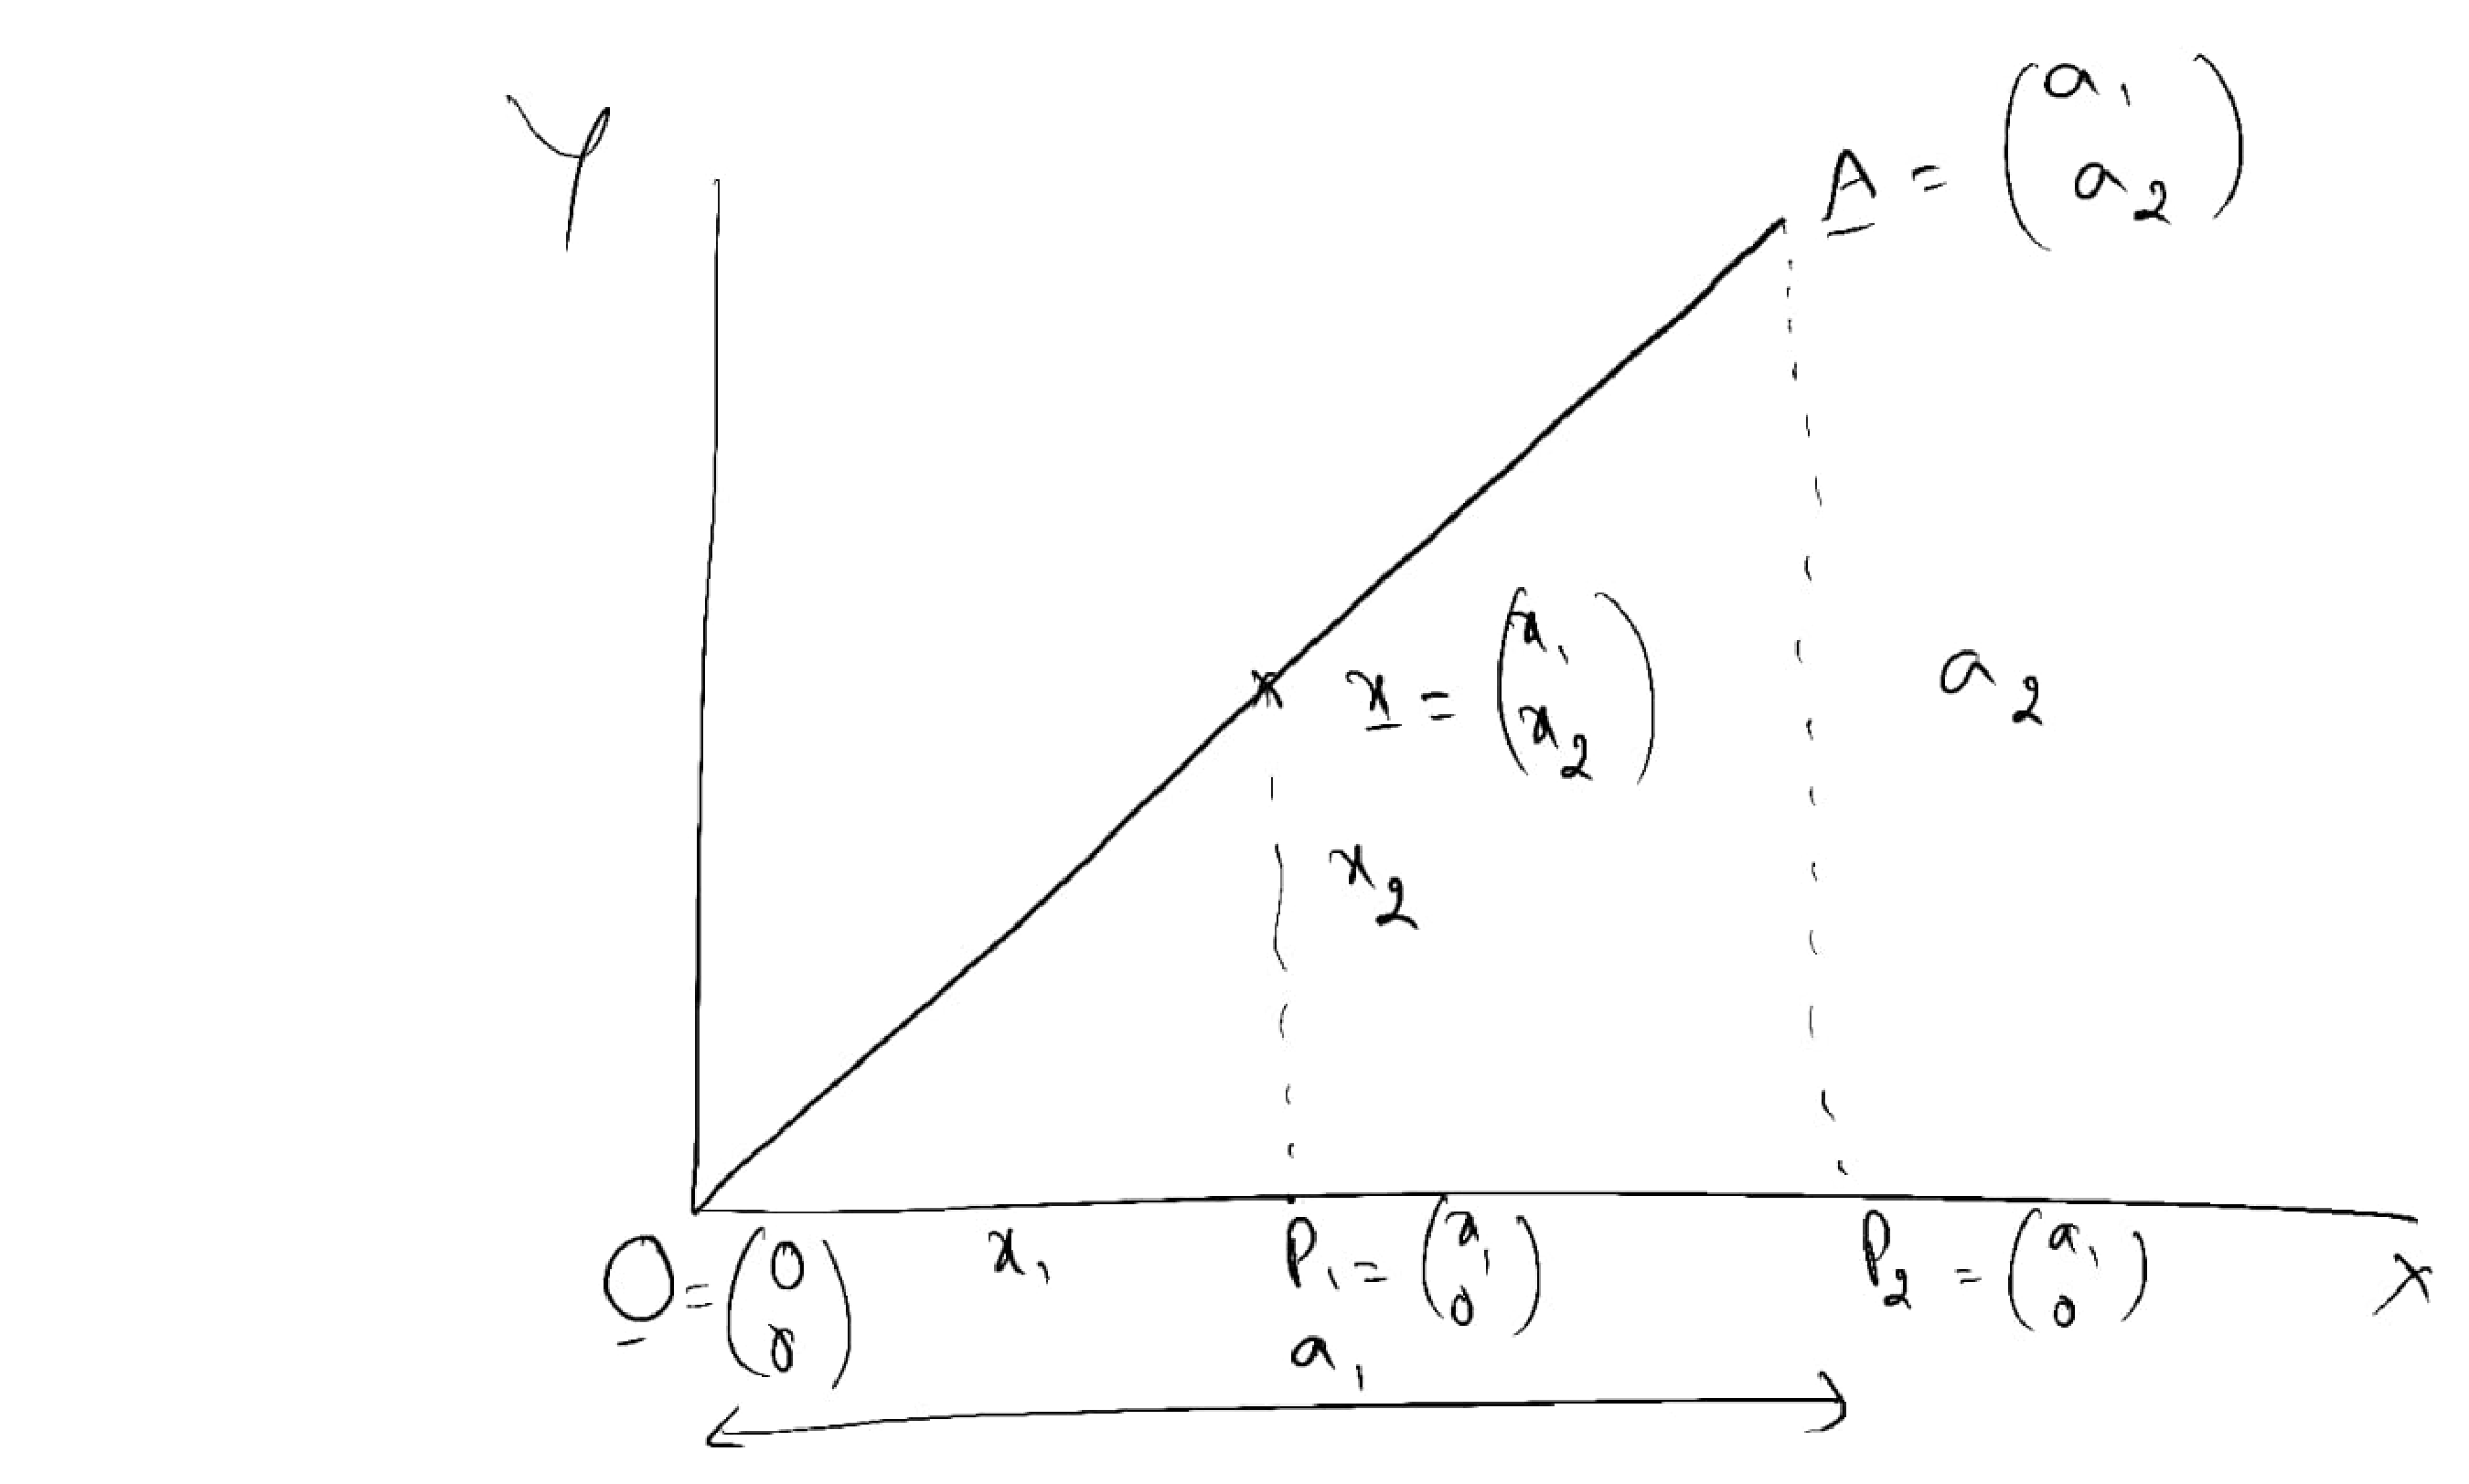
\includegraphics[width=\columnwidth]{./figs/line_homog.eps}
\caption{}
\label{fig:line_homog}
\end{figure}
\\
\solution
Let $\vec{x}=\myvec{x_1\\x_2}$ be any point on $OA$.
Then, using similar triangles,
\begin{align}
\frac{x_2}{x_1} &= \frac{a_2}{a_1} = m
\\
\implies x_2 &=  m x_1
\end{align}
where $m$ is known as the slope of the line. Thus, the equation of the line is
\begin{align}
%\label{eq:homog}
\vec{x} = \myvec{x_1\\m x_1} = x_1 \myvec{1 \\ m} = x_1\vec{m}
\end{align}
In general, the above equation is written as
\begin{align}
\label{eq:homog}
\vec{x} = \lambda \vec{m},
\end{align}
%
where $\vec{m}$ is the direction vector of the line.

\item Find the equation of $AB$ in Fig. \ref{fig:line_nhomog}
\begin{figure}
\centering
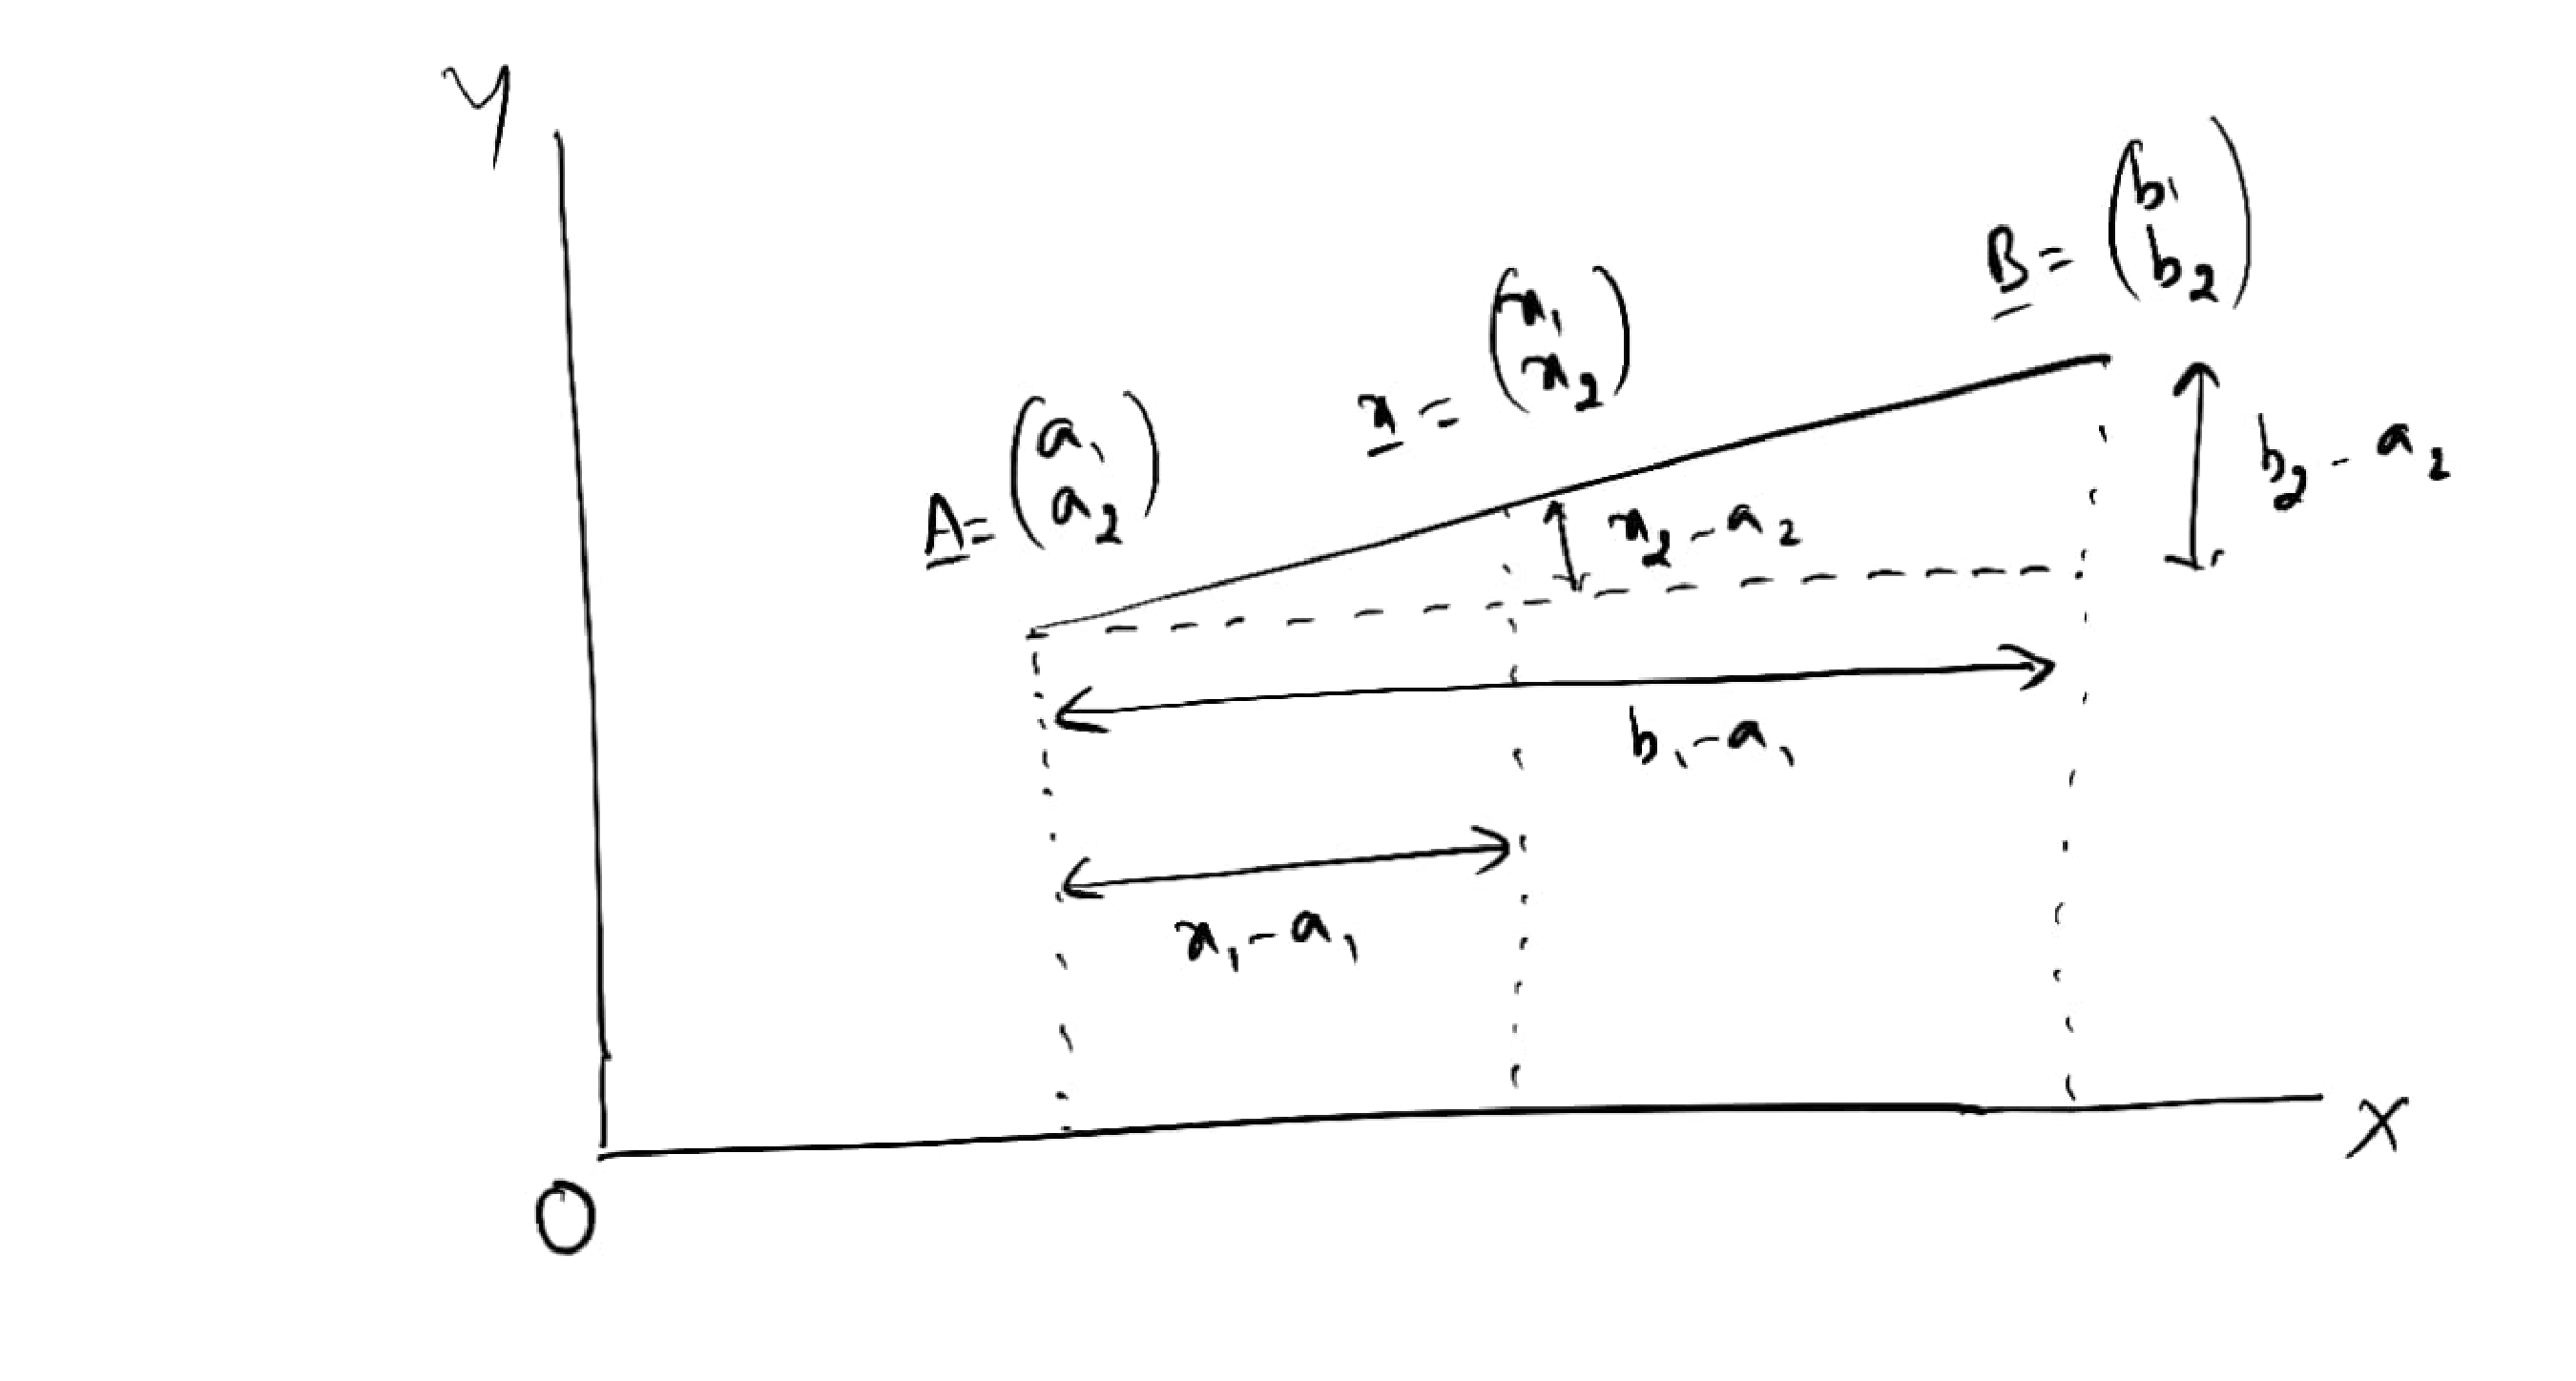
\includegraphics[width=\columnwidth]{./figs/line_nhomog.eps}
\caption{}
\label{fig:line_nhomog}
\end{figure}
\\
\solution 
From Fig. \ref{fig:line_nhomog}, 
%
\begin{align}
\frac{x_2-a_2}{x_1-a_1} = \frac{b_2-a_2}{b_1-a_1} = m
\\
\implies x_2 = m x_1 + a_2-ma_1
\label{eq:line_shift}
\end{align}
%
From \eqref{eq:line_shift},
\begin{align}
\myvec{x_1 \\ x_2} &= 
\myvec{x_1 \\   m x_1 + a_2-ma_1
} 
\\
&=\vec{A} + \brak{x_1-a_1}  \myvec{1 \\ m}
\\
&=\vec{A} + \lambda  \vec{m}
\label{eq:nhomog}
\end{align}
\item {\em Translation:} If the line shifts from the origin by $\vec{A}$, \eqref{eq:nhomog} is obtained from \eqref{eq:homog} by adding $\vec{A}$.
\item Find the length of $\vec{A}$ in Fig. \ref{fig:line_homog}
\\
\solution Using Baudhayana's theorem, the length of the vector $\vec{A}$ is defined as
\begin{equation}
 \norm{\vec{A}} = OA = \sqrt{a_1^2 + a_2^2}
=\sqrt{\vec{A}^T\vec{A}}.
\end{equation}
%
Also, from \eqref{eq:homog}, 
\begin{equation}
\norm{\vec{A}} = \lambda \sqrt{1+m^2}
\end{equation}
%
Note that $\lambda$ is the variable that determines the length of $\vec{A}$, 
since $m$ is constant for all points on the line.
%
\item Find $\vec{A}-\vec{B}$.
\begin{figure}
\centering
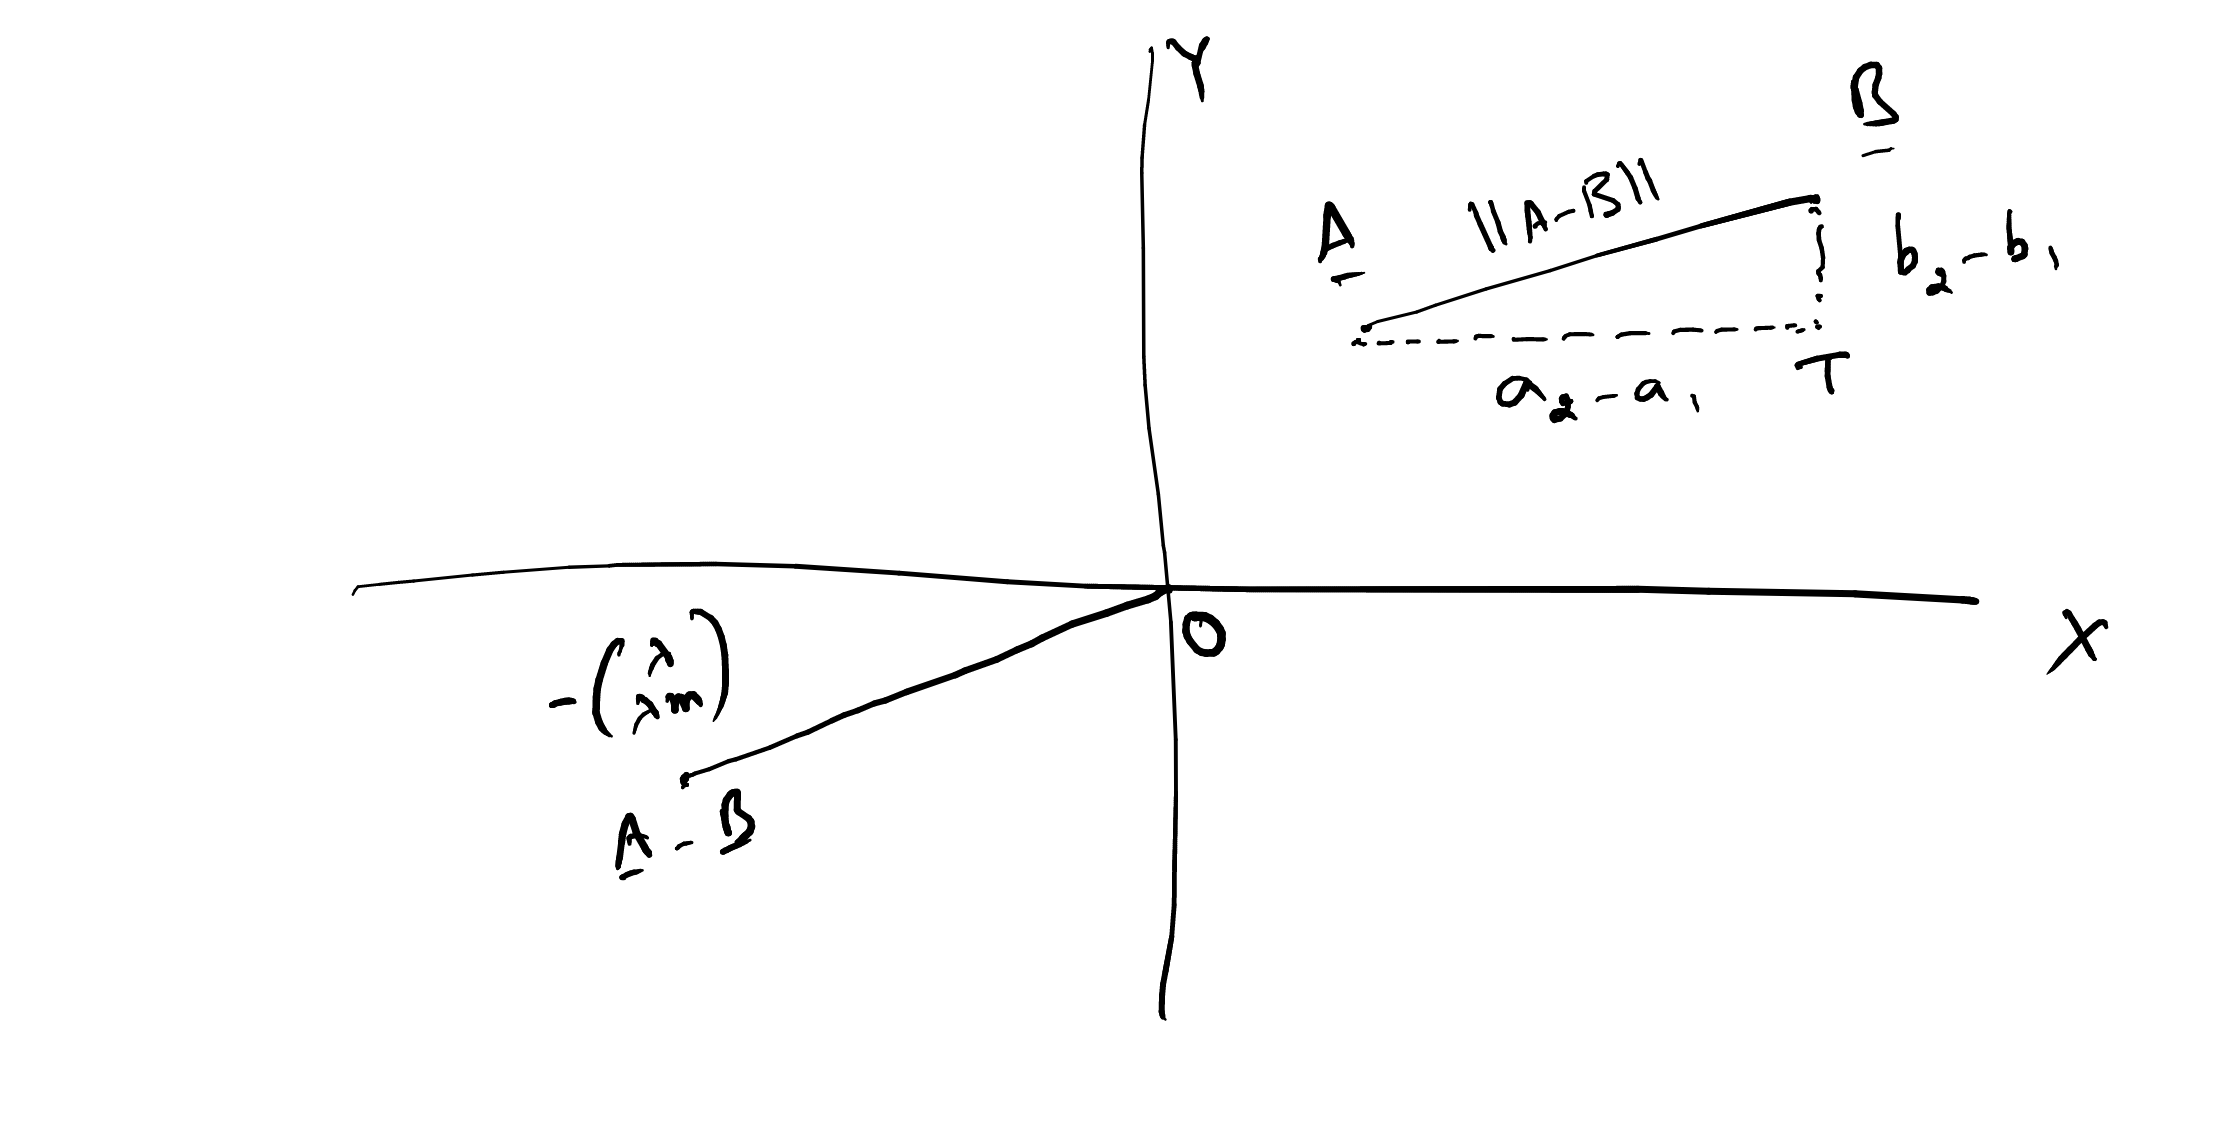
\includegraphics[width=\columnwidth]{./figs/ab.eps}
\caption{}
\label{fig:ab}
\end{figure}
%
\\
\solution See Fig. \ref{fig:ab}. From \eqref{eq:nhomog}, for some 
$\lambda$,
\begin{align}
\vec{B} &=\vec{A} + \lambda \myvec{1 \\ m}
\\
\implies \vec{A} - \vec{B} &= - \lambda \myvec{1 \\ m},
\end{align}
%
$\vec{A} - \vec{B}$ is marked in Fig. \ref{fig:ab}.
%
\item Show that $AB = \norm{\vec{A}-\vec{B}}$
\item Show that the equation of $AB$ is
\begin{align}
\label{eq:line_ab}
\vec{x} = \vec{A}+ \lambda\brak{\vec{B}-\vec{A}}
\end{align}
%
\item The {\em normal} to the vector $\vec{m}$ is defined as
\begin{align}
\label{eq:normal}
\vec{n}^T\vec{m} = 0
\end{align}
\begin{align}
\label{eq:normal_omat}
\vec{n} = \myvec{0 & 1\\ -1 & 0}\vec{m}
\end{align}
\item From \eqref{eq:line_ab}, the equation of a line can also be expressed as
\begin{align}
\label{eq:line_ab_normal}
\vec{n}^T\vec{x} &= \vec{n}^T\vec{A}+ \lambda\vec{n}^T\brak{\vec{B}-\vec{A}}
\\
\implies \vec{n}^T\vec{x} &=c
\label{eq:line_normal}
\end{align}
\item The unit vectors on the $x$ and $y$ axis are defined as
\begin{align}
\label{eq:line_unit}
\vec{e}_1 &=\myvec{1\\0}, 
\\
\vec{e}_2 &=\myvec{0\\1}
\end{align}
\item If $a$ be the {\em intercept} of the line 
\begin{align}
\label{eq:line_intercept}
\vec{n}^T\vec{x} &=c
\end{align}
on the $x-$axis, then $\myvec{a\\0}$  is a point on the line.  Thus, 
\begin{align}
%\label{eq:line_intercept}
\vec{n}^T\myvec{a\\0} &=c
\\
\implies a &= \frac{c}{\vec{n}^T\vec{e}_1}
\end{align}
%
\renewcommand{\theequation}{\theenumi}
%
\item The {\em rotation matrix} is defined as
\begin{align}
\vec{Q} = \myvec{\cos \theta & -\sin \theta\\ \sin \theta & \cos \theta}
\end{align}
%
where $\theta$ is anti-clockwise.
\item 
\begin{align}
\vec{Q}^T\vec{Q} = \myvec{1 & 0 \\ 0 & 1} = \vec{I}
\end{align}
%
where $\vec{I}$ is the {\em identity matrix}. The rotation matrix $\vec{Q}$ is also an {\em orthogonal matrix}.

\numberwithin{equation}{enumi}
%
\item Find the equation of  line $L$ in Fig. \ref{fig:line_dist}.
\\
\solution The equation of the $x-$axis is
\begin{align}
\vec{x} =\lambda \vec{e}_1
\end{align}
Translation by $p$ units along the $y-$axis results in 
\begin{align}
L_0: \quad \vec{x} = \lambda \vec{e}_1 + p \vec{e}_2 
\end{align}
Rotation by $90\degree-\alpha$ in the anti-clockwise direction yields
\begin{align}
L: \quad \vec{x} &= \vec{Q}\cbrak{\lambda \vec{e}_1 + p \vec{e}_2 }
\\
&=\lambda \vec{Q}\vec{e}_1 + p \vec{Q}\vec{e}_2 
\label{eq:line_dist_temp}
\end{align}
%
where 
\begin{align}
\vec{Q} &= \myvec{\cos \brak{\alpha-90} & -\sin \brak{\alpha-90}\\ \sin \brak{\alpha-90} & \cos \brak{\alpha-90}}
\\
&= \myvec{\sin \alpha & \cos \alpha \\ -\cos \alpha & \sin \alpha}
\end{align}
%
From \eqref{eq:line_dist_temp},
\begin{align}
L: \quad \vec{e}_2^T\vec{Q}^T\vec{x}&=\lambda \vec{e}_2^T\vec{Q}^T\vec{Q}\vec{e}_1 + p \vec{e}_2^T\vec{Q}^T\vec{Q}\vec{e}_2 
\nonumber \\
&=\lambda \vec{e}_2^T\vec{e}_1 + p \vec{e}_2^T\vec{e}_2 
\end{align}
resulting in 
\begin{align}
L: \quad \myvec{\cos \alpha & \sin \alpha}\vec{x}=p
\label{eq:line_dist_temp_final}
\end{align}
\begin{figure}
\centering
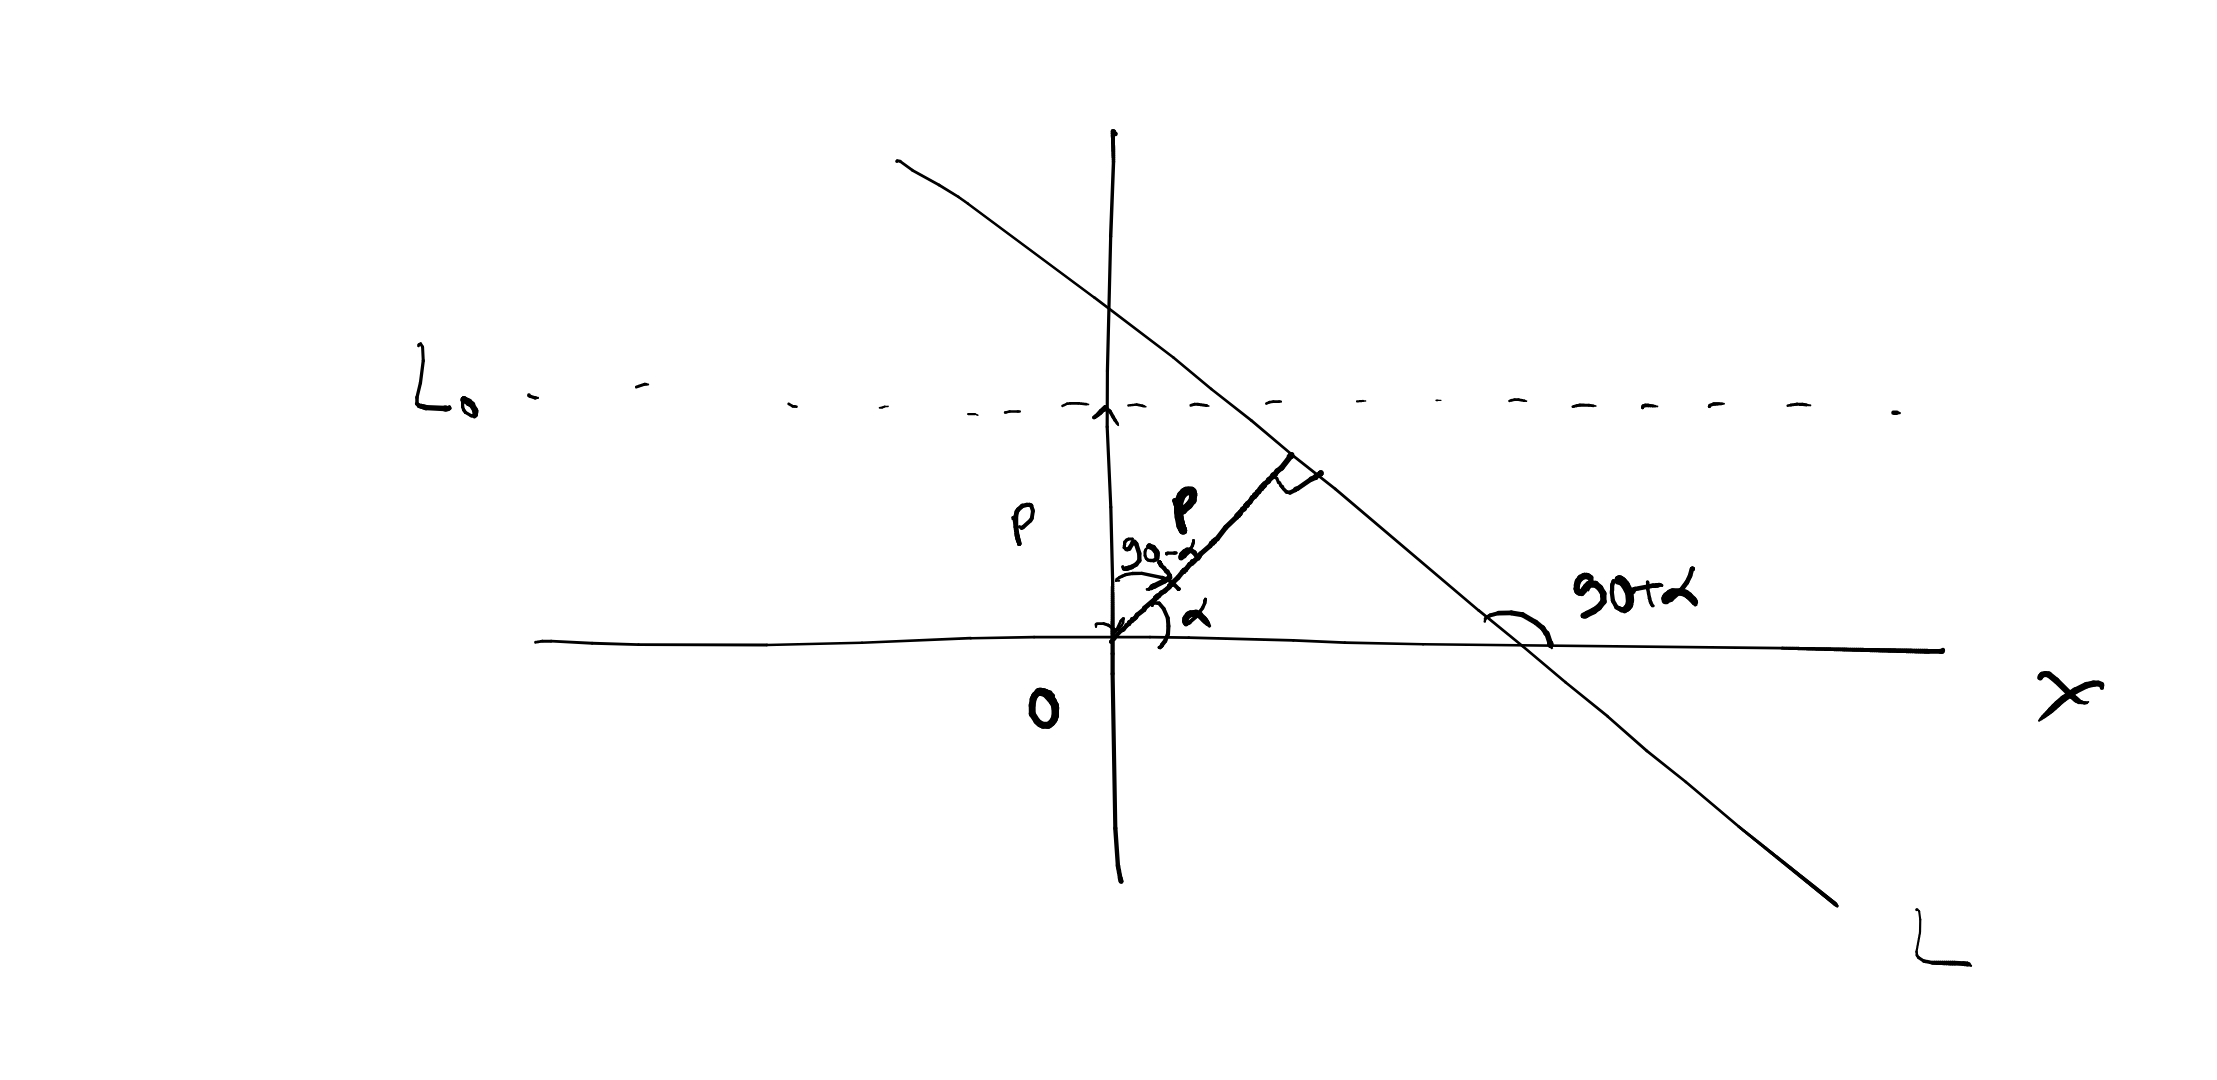
\includegraphics[width=\columnwidth]{./figs/line_dist.eps}
\caption{}
\label{fig:line_dist}
\end{figure}
\item Show that the distance from the orgin to the line 
\begin{align}
\vec{n}^T\vec{x} &=c
\end{align}
is 
\begin{align}
p = \frac{c}{\norm{n}}
\label{eq:line_dist_orig}
\end{align}
\item Show that the point of intersection of two lines 
\begin{align}
\vec{n}_1^T\vec{x} &=c_1
\\
\vec{n}_2^T\vec{x} &=c_2
\end{align}
is given by 
\begin{align}
\vec{x} &=\brak{\vec{N}^T}^{-1}\vec{c}
\end{align}
where 
\begin{align}
\vec{N} = \myvec{\vec{n}_1 & \vec{n}_2}
\end{align}
\item The {\em angle between two lines} is given by 
\begin{align}
\cos ^{-1} \frac{\vec{n}_1 ^T \vec{n}_2}{\norm{\vec{n}_1}  \norm{\vec{n}_2}}
\end{align}
\item Show that the distance of a point $\vec{x}_0$ from the line 
\begin{align}
L: \quad \vec{n}^T\vec{x} &=c
\end{align}
is 
\begin{align}
\frac{\abs{\vec{n}^T\vec{x}_0-c}}{\norm{\vec{n}}} 
\end{align}
\solution Let the equation of the line be 
\begin{align}
\vec{x} = \vec{A} + \lambda \vec{m}
\end{align}
%
where 
\begin{align}
\label{eq:line_dist_orig_pt}
\vec{n}^T\vec{A} = 0, \vec{n}^T\vec{m} = 0
\end{align}
If $\vec{x}_0$ is translated to the origin, the equation of the line $L$ becomes 
\begin{align}
\vec{x} &= \vec{A}- \vec{x}_0+ \lambda \vec{m}
\\
\implies 
\vec{n}^T\vec{x} &=c-\vec{n}^T\vec{x}_0
\end{align}
From \eqref{eq:line_dist_orig}, \eqref{eq:line_dist_orig_pt} is obtained.
\item Show that 
\begin{align}
ax^2+2bxy+cy^2+2dx+2ey+f=0
\end{align}
can be expressed as
\begin{align}
\label{eq:quad_form}
\vec{x}^T\vec{V}\vec{x}+2\vec{u}^T\vec{x}+f=0
\end{align}
%
where
\begin{align}
\vec{V} &= \vec{V}^T
\\
\vec{u} &= \myvec{d & e}
\end{align}

\item {\em Pair of straight lines:} \eqref{eq:quad_form}
%The equation
%\begin{align}
%\vec{x}^T\myvec{a & b\\ b & c}\vec{x}+2\myvec{d & e}+f=0
%\end{align}
%
represents a pair of straight lines if 
\begin{align}
\begin{vmatrix}
\vec{V}&\vec{u}
\\
\vec{u}^T&f
\end{vmatrix}
= 0
\end{align}
%
Two intersecting lines are obtained if 
\begin{align}
\abs{\vec{V}} < 0
\end{align}
\item  In Fig. \ref{fig:ratio}, let
\begin{equation}
\frac{AB}{BC} = \frac{\norm{\vec{A}-\vec{B}}}{\norm{\vec{B}-\vec{C}}} = k.
\label{eq:k}
\end{equation}
%
Show that
\begin{equation}
\frac{\vec{A}+k\vec{C}}{k+1} = \vec{B}.
\label{eq:ratio}
\end{equation}
%
\solution
%
\begin{figure}[!hb]
\centering
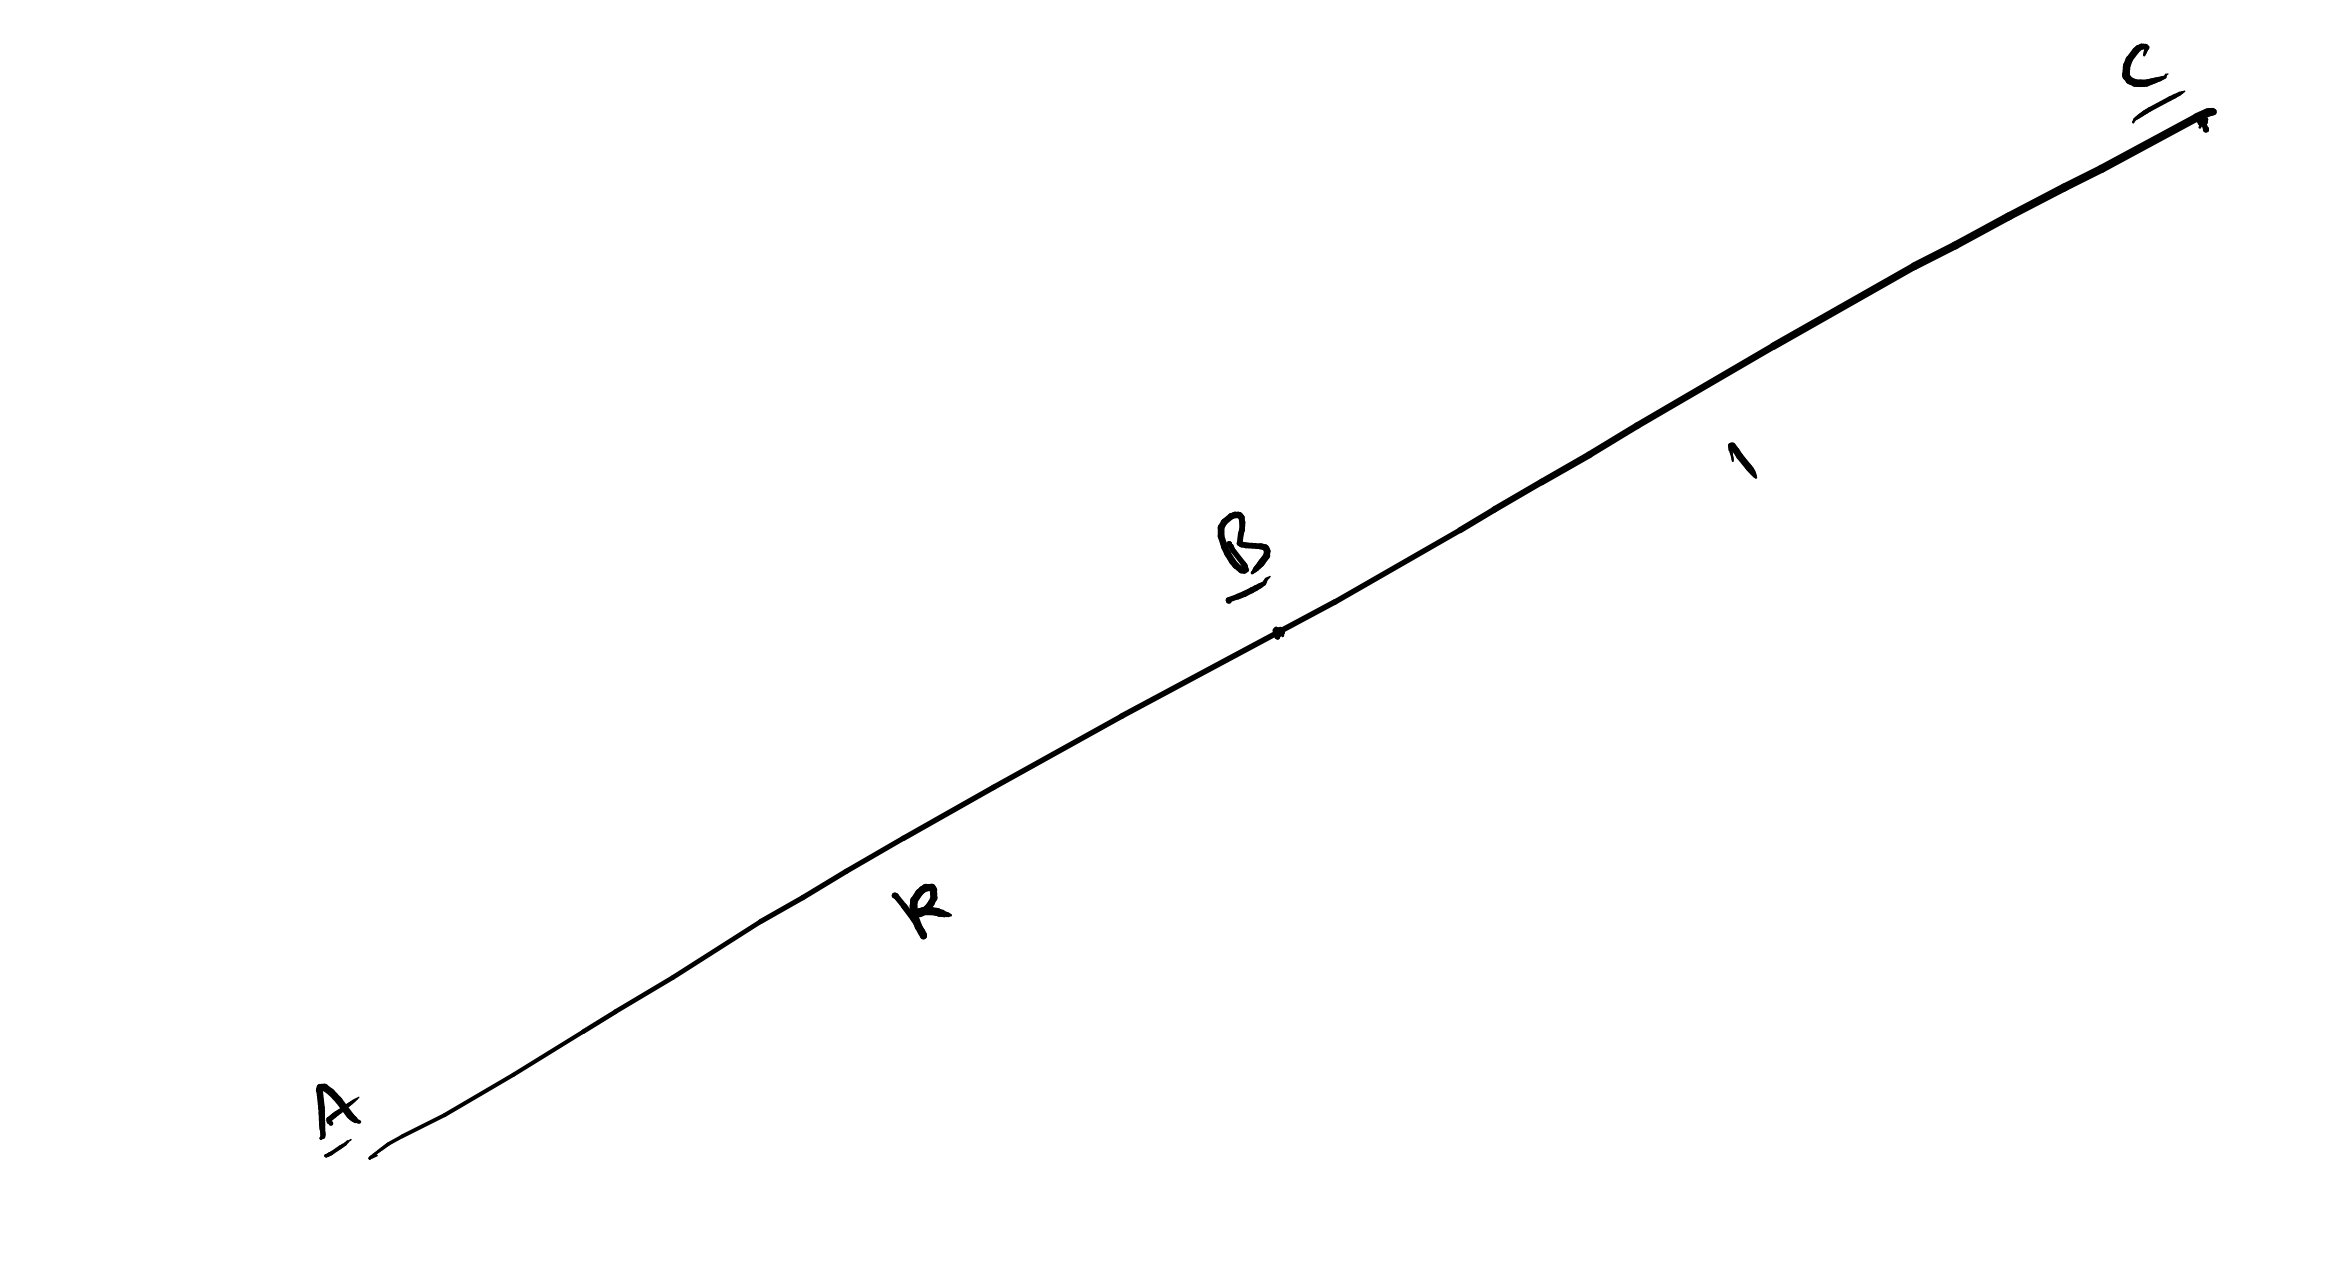
\includegraphics[width=\columnwidth]{./figs/ratio.eps}
\caption{}
\label{fig:ratio}
\end{figure}
From \eqref{eq:nhomog}, 
\begin{align}
\begin{split}
\vec{B} &= \vec{A} + \lambda_1 \vec{m}
\\
\vec{B} &= \vec{C} - \lambda_2 \vec{m}
\end{split}
\\
\label{eq:rat_1}
\implies \frac{\norm{\vec{A}-\vec{B}}}{\norm{\vec{B}-\vec{C}}} &= 
\frac{\lambda_1}{\lambda_2} = k
\\
\text{and } \frac{\vec{B}- \vec{A}}{\lambda_1} &= \frac{\vec{C}- 
\vec{B}}{\lambda_2} = \vec{m},
\label{eq:rat_2}
\end{align}
%
from \eqref{eq:k}. Using \eqref{eq:rat_1} and \eqref{eq:rat_2},
\begin{align}
\vec{A}- \vec{B} &=  k\brak{\vec{B}- \vec{C}}
\end{align}
%
resulting in \eqref{eq:ratio}

%
\item If $\vec{A}$ and $\vec{B}$ are linearly independent,  
\begin{equation}
k_1\vec{A} + k_2\vec{B} = 0 \implies k_1=k_2=0
\end{equation}
\item Show that $\vec{D}$ lies inside $\triangle ABC$ iff
\begin{align}
\vec{D} = \lambda_1\vec{A} + \lambda_2\vec{B} + \lambda_3\vec{C}
\end{align}
such that
\begin{align}
0 \le \lambda_1, \lambda_2, \lambda_3 &\le 1,
\\
0 \le \lambda_1+\lambda_2+\lambda_3 &\le 1,
\end{align}
\item Show that the equation of the angle bisectors of the lines
\begin{align}
\vec{n}_1^T\vec{x} &=c_1
\\
\vec{n}_2^T\vec{x} &=c_2
\end{align}
%
is
\begin{align}
\frac{\vec{n}_1^T\vec{x}-c_1}{\norm{\vec{n}_1}}=\pm\frac{\vec{n}_2^T\vec{x} -c_2}{\norm{\vec{n}_2}}\end{align}
%\item Show that if 
%\begin{align}
%\vec{m}_1 + k\vec{m}_2 \ne 0,
%\end{align}
%%
%there exists $k$ such that for any point $\vec{m}$,
%\begin{align}
%\label{eq:line_basis}
%\vec{m} = \vec{m}_1 + k\vec{m}_2 
%\end{align}
\item Find the equation of a line passing through the intersection of the lines
\begin{align}
\label{eq:line1}
\vec{n}_1^T\vec{x} &=c_1
\\
\vec{n}_2^T\vec{x} &=c_2
\label{eq:line2}
\end{align}
and passing through the point $\vec{p}$.
\\
\solution 
%Let the equation of any line through the intersection of \eqref{eq:line1} and \eqref{eq:line2} be 
%\begin{align}
%\vec{n}^T\vec{x} &=c
%\label{eq:line12}
%\end{align}
%
%If $\vec{u}$ be the point of intersection, 
%\begin{align}
%\myvec{\vec{n}_1^T\\ \vec{n}_2^T\\ \vec{n}^T}\vec{u} &= \myvec{c_1\\c_2\\c}
%\\
%\implies \myvec{\vec{n}_1^T & c_1\\ \vec{n}_2^T & c_2\\ \vec{n}^T & c}&
%\label{eq:line12_mat}
%\end{align}
%has rank 2.  Thus, 
%%
%\begin{align}
%\label{eq:line_basis_normal}
%\myvec{\vec{n}\\c} &= k_1\myvec{\vec{n}_1 \\ c_1}+ k_2\myvec{\vec{n}_2\\c_2} 
%\end{align}
%Substituting in \eqref{eq:line12},
%\begin{align}
%\vec{n}^T\vec{x} = c &
%\implies \vec{n}_1^T\vec{x} + k\vec{n}_2^T\vec{x} =  c_1+kc_2=c
%\label{eq:line_basis_normal_temp}
%\end{align}
%%
%Thus, 
%\begin{align}
%k = \frac{\vec{n}_1^T\vec{p}-c_1}{\vec{n}_2^T\vec{p}-c_2}
%\end{align}
%%
%which can be used to obtain the desired equation using \eqref{eq:line_basis_normal_temp}
%
%Alternatively, 
%
%
The intersection of the lines is 
\begin{align}
\vec{x} = \vec{N}^{-T}\vec{c}
\end{align}
%
where 
\begin{align}
\vec{N} &= \myvec{\vec{n}_1 &\vec{n}_2}
\\
\vec{c} &= \myvec{c_1 \\ c_2} 
\end{align}
Thus, the equation of the desired line is 
\begin{align}
\vec{x} = \vec{p}+ \lambda\brak{\vec{N}^{-T}\vec{c}-\vec{p}}&
\\
\implies \vec{N}^{T}\vec{x} = \vec{N}^{T}\vec{p}+ \lambda\brak{\vec{c}-\vec{N}^{T}\vec{p}}&
\end{align}
resulting in 
\begin{multline}
 \brak{\vec{c}-\vec{N}^T\vec{p}}^T\myvec{0 & -1 \\ 1 & 0}\vec{N}^T\vec{x} 
\\
= \brak{\vec{c}-\vec{N}^T\vec{p}}^T\myvec{0 & -1 \\ 1 & 0}\vec{N}^T\vec{p}
\end{multline}
\item Find $\vec{R}$, the {\em reflection}  of $\vec{P}$ about the line
\begin{align}
L: \quad \vec{n}^T\vec{x} = c
\end{align}
%
\begin{figure}
\centering
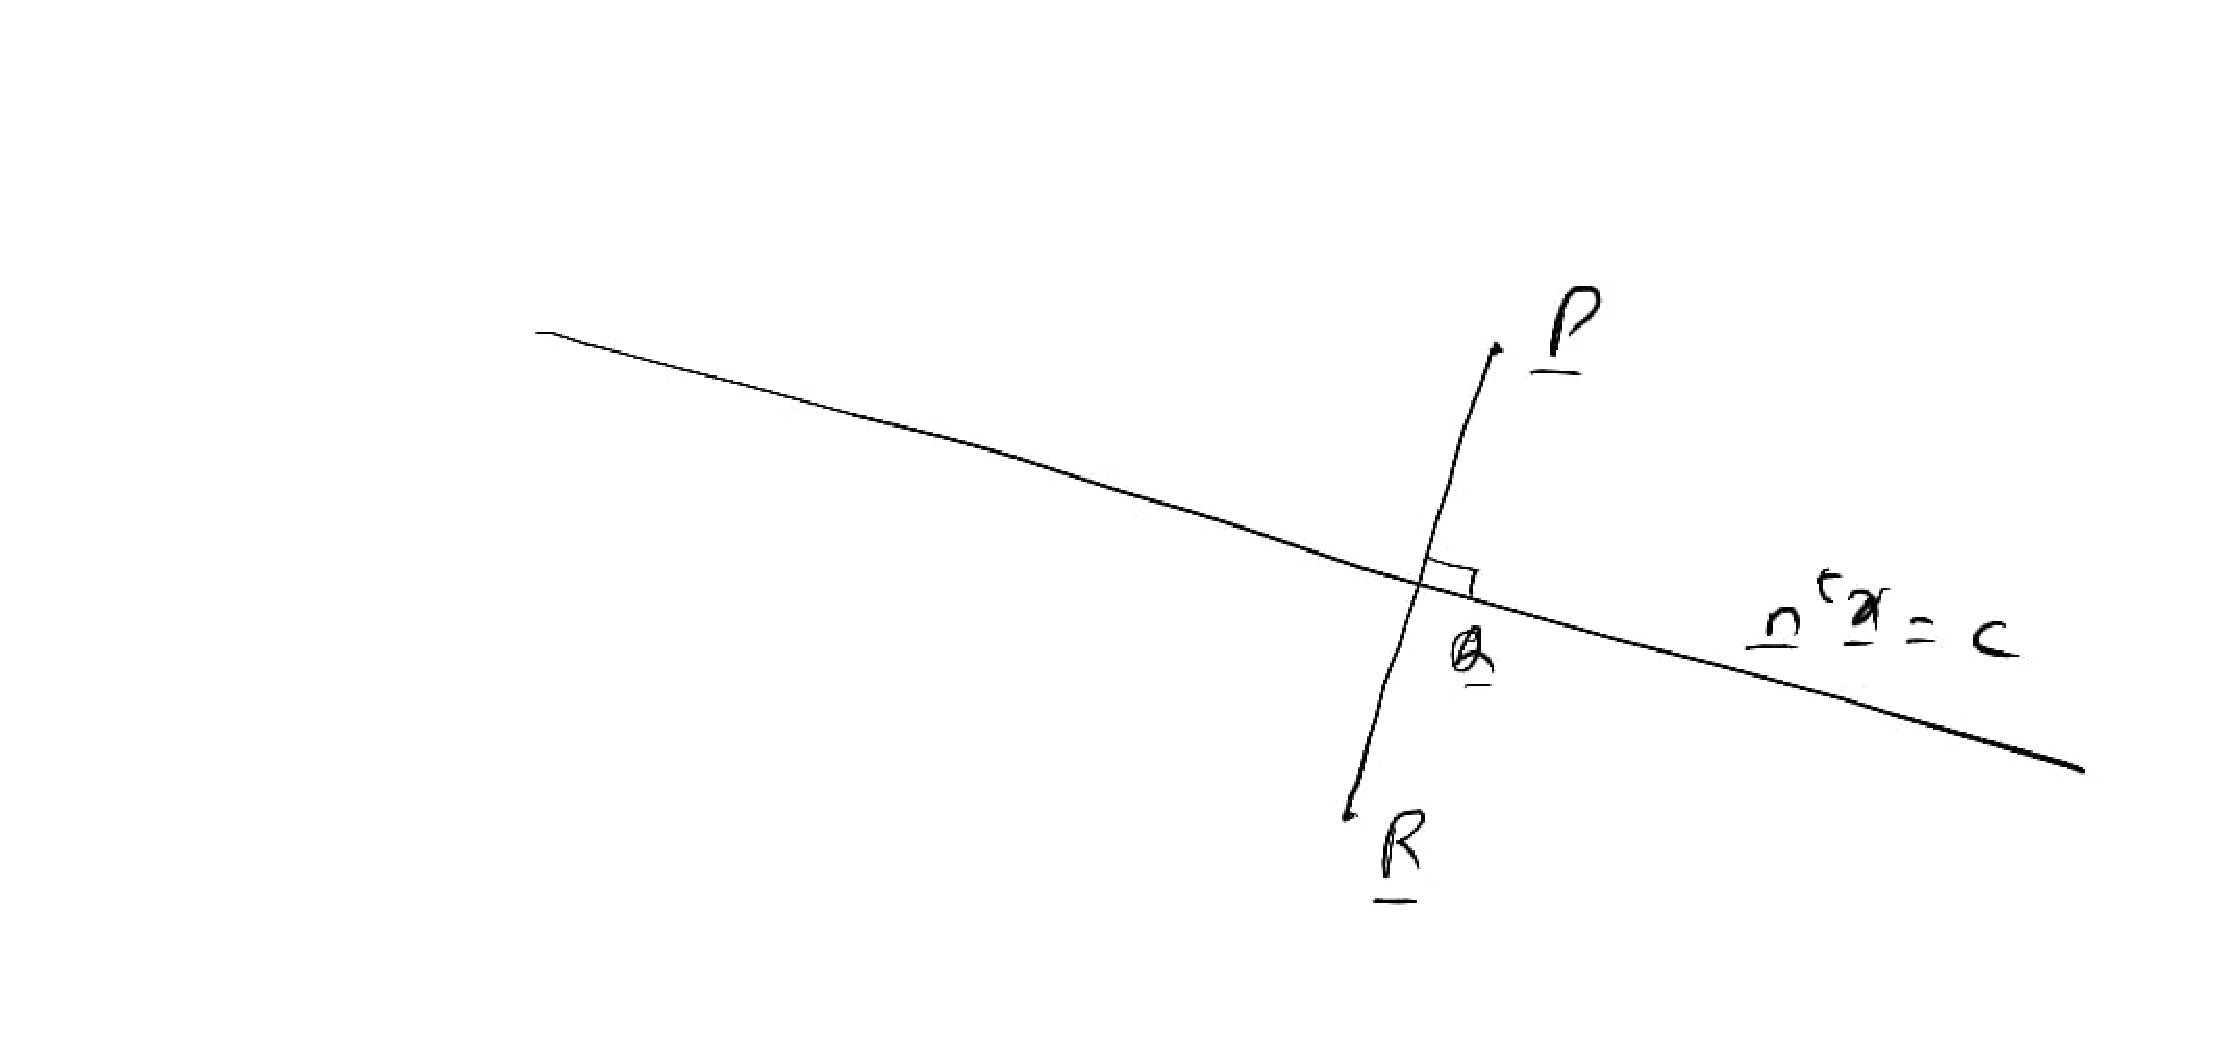
\includegraphics[width=\columnwidth]{./figs/reflection.eps}
\caption{}
\label{fig:locus}
\end{figure}
\solution Since $\vec{R}$ is the reflection of $\vec{P}$ and $\vec{Q}$ lies on $L$, $\vec{Q}$ bisects $PR$.  
This leads to the following equations
Hence, 
\begin{align}
\label{eq:reflect_bisect}
2\vec{Q} &= \vec{P}+\vec{R}
\\
\label{eq:reflect_Q}
\vec{n}^{T}\vec{Q} &= c
\\
\label{eq:reflect_R}
\vec{m}^{T}\vec{R} &= \vec{m}^{T}\vec{P}
\end{align}
%
where $\vec{m}$ is the direction vector of $L$.  From \eqref{eq:reflect_bisect} and \eqref{eq:reflect_Q},
\begin{align}
\label{eq:reflect_bisectQ}
\vec{n}^{T}\vec{R}  &= 2c - \vec{n}^{T}\vec{P}
\end{align}
%
From \eqref{eq:reflect_bisectQ} and \eqref{eq:reflect_R},
\begin{align}
\label{eq:reflect_bisectQR}
\myvec{\vec{m} & \vec{n}}^T\vec{R} &= \myvec{\vec{m} & -\vec{n}}^T\vec{P}+ \myvec{0 \\ 2c}
\end{align}
%
Letting 
\begin{align}
\label{eq:reflect_mat}
\vec{V}=  \myvec{\vec{m} & \vec{n}}
\end{align}
with the condition that $\vec{m},\vec{n}$ are orthonormal, i.e.
\begin{align}
\label{eq:reflect_ortho}
\vec{V}^T\vec{V}=  \vec{I}
\end{align}
%
Noting that 
\begin{align}
\label{eq:reflect_trans}
\myvec{\vec{m} & -\vec{n}} &= \myvec{\vec{m} & \vec{n}} \myvec{1 & 0 \\ 0 & -1},
\end{align}
\eqref{eq:reflect_bisectQR} can be expressed as
%
\begin{align}
\label{eq:reflect_}
\vec{V}^T\vec{R} &=  \sbrak{\vec{V}\myvec{1 & 0 \\ 0 & -1}}^T\vec{P}+\myvec{0 \\ 2c}
\\
\implies \vec{R} &= \sbrak{\vec{V}\myvec{1 & 0 \\ 0 & -1}\vec{V}^{-1}}^T\vec{P}+ \vec{V}\myvec{0 \\ 2c}
\\
 &=\vec{V}\myvec{1 & 0 \\ 0 & -1}\vec{V}^T \vec{P}+2c \vec{n}
\end{align}
\item Show that, for any $\vec{m},\vec{n}$, the reflection is also given by
\begin{align}
%\label{eq:reflect_bisect}
\frac{\vec{R}}{2} = \frac{\vec{m}\vec{m}^T-\vec{n}\vec{n}^T}{\vec{m}^T\vec{m}+\vec{n}^T\vec{n}}\vec{P} + c 
\frac{\vec{n}}{\norm{\vec{n}}^2}
\end{align}

\end{enumerate}
%
%
%\item Let $\vec{x}$ be any point on $AB$ in Fi.g \ref{fig:orth}.  Show that
%\begin{equation}
%\brak{\vec{x}-\vec{A}}^T\brak{\vec{B}-\vec{C}} = 0
%\end{equation}
%%
%\item If $\vec{x,y}$ are any two points on $AB$, show that 
%\begin{equation}
%\label{eq:orth_any}
%\brak{\vec{x}-\vec{y}}^T\brak{\vec{B}-\vec{C}} = 0
%\end{equation}
%%
%\item In Fig. \ref{fig:alt}, $BE \perp AC, CF \perp AB$.  Show that $AD \perp BC$.
%\begin{figure}[!hb]
%\centering
%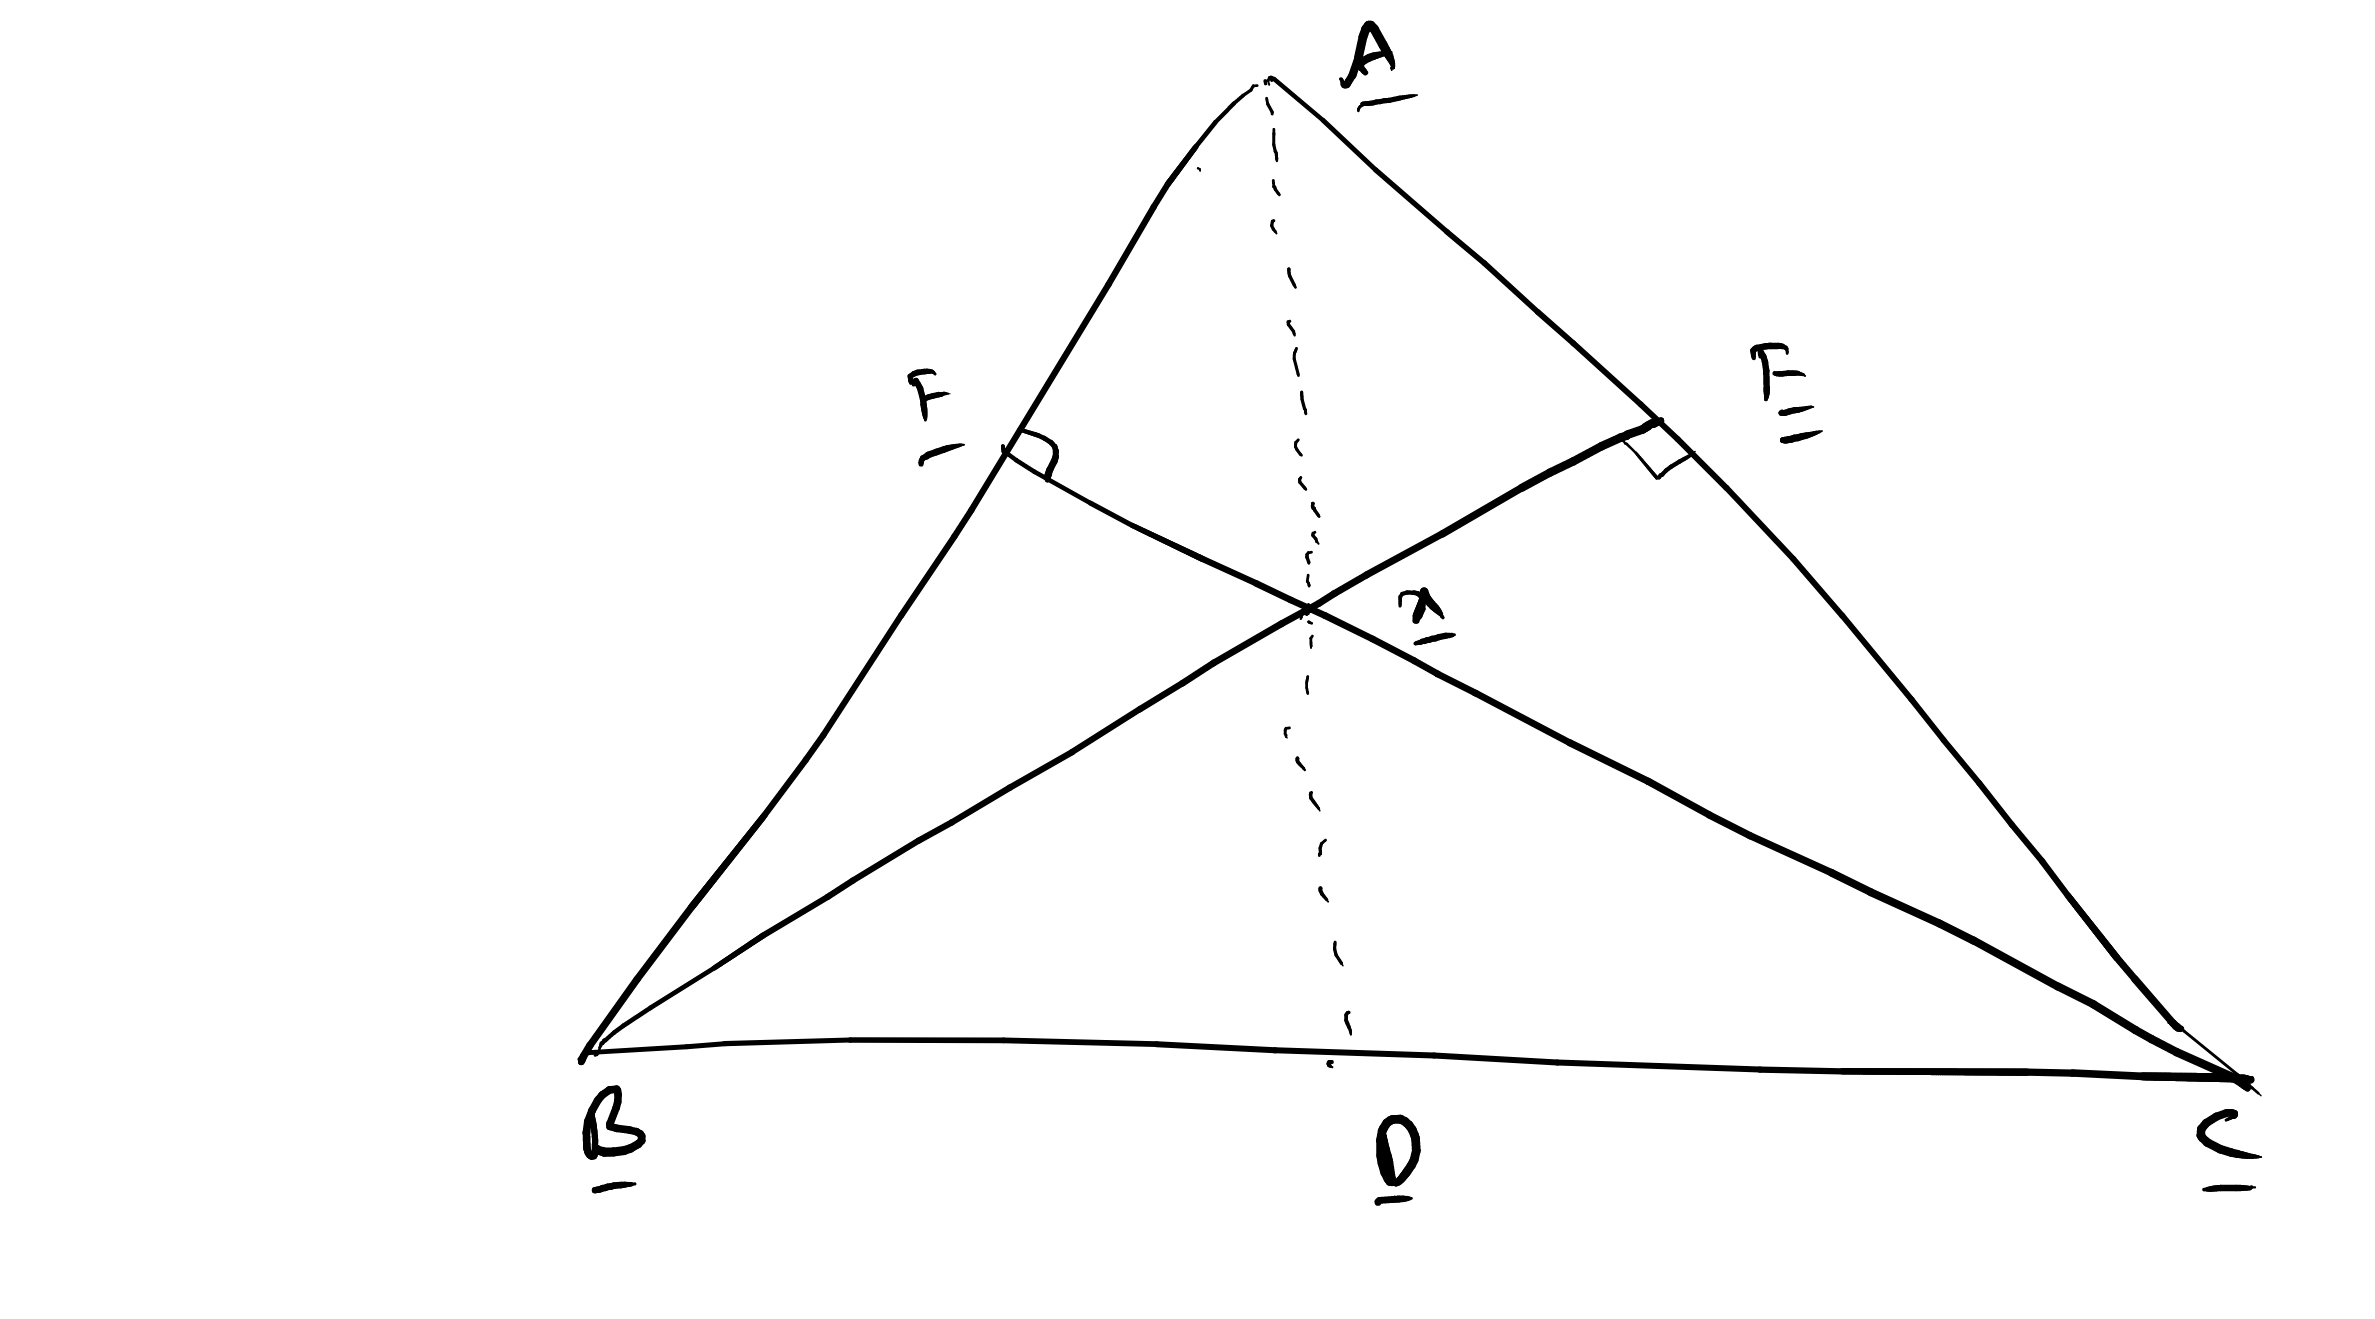
\includegraphics[width=\columnwidth]{./figs/alt.eps}
%\caption{}
%\label{fig:alt}
%\end{figure}
%\\
%\solution Let $\vec{x}$ be the intersection of $BE$ and $CF$. Then, using 
%\eqref{eq:orth_any},
%\begin{align}
%\label{eq:alt_1}
%\begin{split}
%\brak{\vec{x}-\vec{B}}^T
%\brak{\vec{A}-\vec{C}} &= 0
%\\
%\brak{\vec{x}-\vec{C}}^T
%\brak{\vec{A}-\vec{B}} &=0
%\end{split}
%\\
%\label{eq:alt_3}
%\implies \vec{x}^T\brak{\vec{A}-\vec{C}}-\vec{B}^T\brak{\vec{A}-\vec{C}} &= 0
%\\
%\text{and }\vec{x}^T\brak{\vec{A}-\vec{B}}-\vec{C}^T\brak{\vec{A}-\vec{B}} &= 0
%\label{eq:alt_4}
%\end{align}
%%
%Subtracting \eqref{eq:alt_4} from \eqref{eq:alt_3},
%\begin{align}
%\vec{x}^T\brak{\vec{B}-\vec{C}} + \vec{A}^T\brak{\vec{C}-\vec{B}} &= 0
%\\
%\implies \brak{\vec{x}^T - \vec{A}^T}\brak{\vec{B}-\vec{C}}  &= 0
%\\
%\implies \brak{\vec{x} - \vec{A}}^T\brak{\vec{B}-\vec{C}}  &= 0
%\end{align}
%%
%which completes the proof.
%\end{enumerate}
%

\subsection{Intercepts}
\renewcommand{\theequation}{\theenumi}
\begin{enumerate}[label=\arabic*.,ref=\thesubsection.\theenumi]
\item Find the intercepts made on the axes by the straight lines whose equations are
\begin{multicols}{2}
\begin{enumerate}
%\begin{enumerate}[(i)]
%\setlength\itemsep{2em}
\item
$
\myvec{2 & 3}\vec{x} = 2
$
\item
$
\myvec{1 & -3}\vec{x} = -5
$ 
\item
$
\myvec{1 & -1}\vec{x} = 0
$
\item
$
\myvec{\frac{1}{a+b} & \frac{1}{a-b}}\vec{x} = \frac{1}{a^2-b^2}
$
\item 
$
\myvec{1 & -m}\vec{x} = -c
$
\end{enumerate}
\end{multicols}
\item Write down the equations of straight lines which make the following pairs of intercepts on the axes:
\begin{multicols}{2}
\begin{enumerate}
\item 3,-4
\item -5,6
\item 
$
\frac{1}{a},\frac{1}{b}
$
\item 
$
2a,-2a
$
\end{enumerate}
\end{multicols}
\item A straight line passes through a fixed point $\myvec{h\\k}$ and cuts the axes in $\vec{A},\vec{B}$.  Parallels to the
axes through $\vec{A}$ and $\vec{B}$ intersect in $\vec{P}$.  Find the equation of the locus of $\vec{P}$.
\end{enumerate}

\subsection{Line Equation}
\renewcommand{\theequation}{\theenumi}
\begin{enumerate}[label=\arabic*.,ref=\thesubsection.\theenumi]
%\begin{enumerate}[1.]
\item Find the equations of two straight lines at a distance 3 from the origin and making an angle of $120 \degree$ with $OX$.
\item Find the equation of a straight line making an angle of $60\degree$ with $OX$ and passing through the point $\myvec{2\\-2}$.
Transform the equation to the form
\begin{equation}
\myvec{\cos\alpha &\sin \alpha}\vec{x} = p 
\end{equation}
\solution
Let the balanced version of (\ref{eq:solutions/chem/6ato balance}) be
\begin{align}
    \label{eq:solutions/chem/6abalanced}x_{1}HNO_{3}+ x_{2}Ca(OH)_{2}\to x_{3}Ca(NO_{3})_{2}+ x_{4}H_{2}O
\end{align}

which results in the following equations:
\begin{align}
    (x_{1}+ 2x_{2}-2x_{4}) H= 0\\
    (x_{1}-2x_{3}) N= 0\\
    (3x_{1}+ 2x_{2}-6x_{3}- x_{4}) O=0\\
    (x_{2}-x_{3}) Ca= 0
\end{align}

which can be expressed as
\begin{align}
    x_{1}+ 2x_{2}+ 0.x_{3} -2x_{4} = 0\\
    x_{1}+ 0.x_{2} -2x_{3} +0.x_{4}= 0\\
    3x_{1}+ 2x_{2}-6x_{3}- x_{4} =0\\
    0.x_{1} +x_{2}-x_{3} +0.x_{4}= 0
\end{align}

resulting in the matrix equation
\begin{align}
    \label{eq:solutions/chem/6a matrix}
    \myvec{1 & 2 & 0 & -2\\
           1 & 0 & -2 & 0\\
           3 & 2 & -6 & -1\\
           0 & 1 & -1 & 0}\vec{x}
           =\vec{0}
\end{align}

where,
\begin{align}
   \vec{x}= \myvec{x_{1}\\x_{2}\\x_{3}\\x_{4}}
\end{align}

(\ref{eq:solutions/chem/6a matrix}) can be reduced as follows:
\begin{align}
    \myvec{1 & 2 & 0 & -2\\
           1 & 0 & -2 & 0\\
           3 & 2 & -6 & -1\\
           0 & 1 & -1 & 0}
    \xleftrightarrow[R_{3}\leftarrow \frac{R_3}{3}-R_{1}]{R_{2}\leftarrow R_2- R_1}
    \myvec{1 & 2 & 0 & -2\\
           0 & -2 & -2 & 2\\
           0 & -\frac{4}{3} & -2 & \frac{5}{3}\\
           0 & 1 & -1 & 0}\\
    \xleftrightarrow{R_2 \leftarrow -\frac{R_2}{2}}
    \myvec{1 & 2 & 0 & -2\\
          0 & 1 & 1 & -1\\
          0 & -\frac{4}{3} & -2 & \frac{5}{3}\\
          0 & 1 & -1 & 0}\\
    \xleftrightarrow[R_4 \leftarrow R_4- R_2]{R_3 \leftarrow R_3 + \frac{4}{3}R_2}
    \myvec{1 & 2 & 0 & -2\\
           0 & 1 & 1 & -1\\
           0 & 0 & -\frac{2}{3} & \frac{1}{3}\\
           0 & 0 & -2 & 1}\\
    \xleftrightarrow[R_3 \leftarrow -\frac{3}{2}R_3]{R_1 \leftarrow R_1- 2R_2}
    \myvec{1 & 0 & -2 & 0\\
           0 & 1 & 1 & -1\\
           0 & 0 & 1 & -\frac{1}{2}\\
           0 & 0 & -2 & 1}\\
    \xleftrightarrow{R_4\leftarrow R_4 + 2R_3}
    \myvec{1 & 0 & -2 & 0\\
           0 & 1 & 1 & -1\\
           0 & 0 & 1 & -\frac{1}{2}\\
           0 & 0 & 0 & 0}\\
    \xleftrightarrow[R_2\leftarrow R_2-R_3]{R_1\leftarrow R_1 + 2R_3}
    \myvec{1 & 0 & 0 & -1\\
           0 & 1 & 0 & -\frac{1}{2}\\
           0 & 0 & 1 & -\frac{1}{2}\\
           0 & 0 & 0 & 0}
\end{align}

Thus,
\begin{align}
    x_1=x_4, x_2= \frac{1}{2}x_4, x_3=\frac{1}{2}x_4\\
    \implies \quad\vec{x}= x_4\myvec{1\\ \frac{1}{2}\\ \frac{1}{2}\\1} =\myvec{2\\1\\1\\2}
\end{align} 
by substituting $x_4= 2$.

\hfill\break
%\vspace{5mm} 
Hence, (\ref{eq:solutions/chem/6abalanced}) finally becomes
\begin{align}
    2HNO_{3}+ Ca(OH)_{2}\to Ca(NO_{3})_{2}+ 2H_{2}O
\end{align}

\item Find the equation of the straight line that passes through the points $\myvec{2\\3}$ and $\myvec{3\\2}$. What is its inclination
to $OX$?
\item Find the equation of the straight line through the point $\myvec{5\\7}$ that makes equal intercepts on the axes.
\item Find the equations of the sides of a triangle whose vertices are $\myvec{2\\4}$, $\myvec{-4\\1}$ and $\myvec{2\\-3}$.
\item For the same triangle find the equations of the medians 
\item Find the equation of a straight line passing through the point $\myvec{2\\-3}$ parallel to the line $\myvec{4 & -1}\vec{x} + 7 =0$.
\item Find the intercepts on the axes made by a straight line which passes through the point $\myvec{3\\-1}$ and makes an angle
of $30\degree$ with $OX$.
\item Find the equation of the straight line through the points $\myvec{3\\-4}$, $\myvec{2\\3}$ and of the
parallel line through $\myvec{5\\2}$.
\item What is the distance from the origin of the line $\myvec{4 & -1}\vec{x} = 7$? Write down the equation of a parallel line at double the distance.
\item Find the equation of the straight line through the point $\myvec{3\\-4}$ parallel to the line joining the origin to the point
$\myvec{2\\-1}$.
\item Write down the equation of the straight line which makes intercepts 2 and -7 on the axes, and of the parallel line through
the point $\myvec{3\\-1}$.
\item Find the equations of the straight line joining the points $\myvec{3\\4}$, $\myvec{-2\\1}$ and of the parallel line through
the origin.
\item $ABC$ is a triangle and $\vec{A}, \vec{B}$ and $\vec{C}$ are the points $\myvec{2\\3}$, $\myvec{5\\-1}$ and $\myvec{-4\\2}$.  Find the equation
of the straight line through $\vec{A}$ parallel to $BC$.
\item Find the equation of a line parallel to $\myvec{2 & 5}\vec{x}=11$ passing through the middle point of the join of the points $\myvec{-7\\3}$, $\myvec{5\\-11}$.
\\
\solution
Let the balanced version of (\ref{eq:solutions/chem/6ato balance}) be
\begin{align}
    \label{eq:solutions/chem/6abalanced}x_{1}HNO_{3}+ x_{2}Ca(OH)_{2}\to x_{3}Ca(NO_{3})_{2}+ x_{4}H_{2}O
\end{align}

which results in the following equations:
\begin{align}
    (x_{1}+ 2x_{2}-2x_{4}) H= 0\\
    (x_{1}-2x_{3}) N= 0\\
    (3x_{1}+ 2x_{2}-6x_{3}- x_{4}) O=0\\
    (x_{2}-x_{3}) Ca= 0
\end{align}

which can be expressed as
\begin{align}
    x_{1}+ 2x_{2}+ 0.x_{3} -2x_{4} = 0\\
    x_{1}+ 0.x_{2} -2x_{3} +0.x_{4}= 0\\
    3x_{1}+ 2x_{2}-6x_{3}- x_{4} =0\\
    0.x_{1} +x_{2}-x_{3} +0.x_{4}= 0
\end{align}

resulting in the matrix equation
\begin{align}
    \label{eq:solutions/chem/6a matrix}
    \myvec{1 & 2 & 0 & -2\\
           1 & 0 & -2 & 0\\
           3 & 2 & -6 & -1\\
           0 & 1 & -1 & 0}\vec{x}
           =\vec{0}
\end{align}

where,
\begin{align}
   \vec{x}= \myvec{x_{1}\\x_{2}\\x_{3}\\x_{4}}
\end{align}

(\ref{eq:solutions/chem/6a matrix}) can be reduced as follows:
\begin{align}
    \myvec{1 & 2 & 0 & -2\\
           1 & 0 & -2 & 0\\
           3 & 2 & -6 & -1\\
           0 & 1 & -1 & 0}
    \xleftrightarrow[R_{3}\leftarrow \frac{R_3}{3}-R_{1}]{R_{2}\leftarrow R_2- R_1}
    \myvec{1 & 2 & 0 & -2\\
           0 & -2 & -2 & 2\\
           0 & -\frac{4}{3} & -2 & \frac{5}{3}\\
           0 & 1 & -1 & 0}\\
    \xleftrightarrow{R_2 \leftarrow -\frac{R_2}{2}}
    \myvec{1 & 2 & 0 & -2\\
          0 & 1 & 1 & -1\\
          0 & -\frac{4}{3} & -2 & \frac{5}{3}\\
          0 & 1 & -1 & 0}\\
    \xleftrightarrow[R_4 \leftarrow R_4- R_2]{R_3 \leftarrow R_3 + \frac{4}{3}R_2}
    \myvec{1 & 2 & 0 & -2\\
           0 & 1 & 1 & -1\\
           0 & 0 & -\frac{2}{3} & \frac{1}{3}\\
           0 & 0 & -2 & 1}\\
    \xleftrightarrow[R_3 \leftarrow -\frac{3}{2}R_3]{R_1 \leftarrow R_1- 2R_2}
    \myvec{1 & 0 & -2 & 0\\
           0 & 1 & 1 & -1\\
           0 & 0 & 1 & -\frac{1}{2}\\
           0 & 0 & -2 & 1}\\
    \xleftrightarrow{R_4\leftarrow R_4 + 2R_3}
    \myvec{1 & 0 & -2 & 0\\
           0 & 1 & 1 & -1\\
           0 & 0 & 1 & -\frac{1}{2}\\
           0 & 0 & 0 & 0}\\
    \xleftrightarrow[R_2\leftarrow R_2-R_3]{R_1\leftarrow R_1 + 2R_3}
    \myvec{1 & 0 & 0 & -1\\
           0 & 1 & 0 & -\frac{1}{2}\\
           0 & 0 & 1 & -\frac{1}{2}\\
           0 & 0 & 0 & 0}
\end{align}

Thus,
\begin{align}
    x_1=x_4, x_2= \frac{1}{2}x_4, x_3=\frac{1}{2}x_4\\
    \implies \quad\vec{x}= x_4\myvec{1\\ \frac{1}{2}\\ \frac{1}{2}\\1} =\myvec{2\\1\\1\\2}
\end{align} 
by substituting $x_4= 2$.

\hfill\break
%\vspace{5mm} 
Hence, (\ref{eq:solutions/chem/6abalanced}) finally becomes
\begin{align}
    2HNO_{3}+ Ca(OH)_{2}\to Ca(NO_{3})_{2}+ 2H_{2}O
\end{align}

\item The base of a triangle passes through a fixed point $\myvec{f\\g}$ and the sides are bisected at right angles by the axes.  Prove that the locus
of the vertex is the line
\begin{equation}
\myvec{g & f}\vec{x} = 0
\end{equation}
\end{enumerate}
 
\subsection{Point of Intersection}
\renewcommand{\theequation}{\theenumi}
\begin{enumerate}[label=\arabic*.,ref=\thesubsection.\theenumi]
\item Find the vertices of the triangle whose sides are
\numberwithin{equation}{enumi}
\begin{align}
\myvec{3 & 2}\vec{x}+6 &= 0,
\\
 \myvec{2 & -5}\vec{x}+4 &= 0,
\\
 \myvec{1 & -3}\vec{x} -6 &= 0
\end{align}
\item Prove that the lines
\begin{align}
\myvec{1 & 1}\vec{x}+25 &= 0, 
\\
\myvec{2 & 3}\vec{x}+7 &= 0 
\\
\myvec{3 & 5}\vec{x} = 11
\end{align}
%
are concurrent, and find the coordinates of their common point.
\item Find the equation of a line parallel to the line 
\begin{align}
\myvec{2 & -1}\vec{x}=3
\end{align}
 and passing through the intersection of the lines
\begin{align}
\myvec{3 & 1}\vec{x}&=7
\\
 \myvec{2 & -3}\vec{x} &= 5
\end{align}
\item Find the equation of the line joining the origin to the point of intersection of the lines
\begin{align}
\myvec{3&-5}\vec{x} &= 11
\\
 \myvec{2&7}\vec{x}+4 &= 0
\end{align}
%
\item Find the acute angle between the lines
\numberwithin{equation}{enumi}
\begin{align}
\myvec{1 & -1} \vec{x}=  - 7 
\\
 \myvec{2+\sqrt{3}& 1} \vec{x}= 11
\end{align}
\item Find the angle between the lines
\begin{align}
\myvec{-2 & 1} \vec{x}&= 5 
\\
 \myvec{2 & 4} \vec{x}+ 11 &= 0
\end{align}
\renewcommand{\theequation}{\theenumi}
\item Find the equation of a straight line through the point $\myvec{2\\-4}$ at right angles to the line 
\begin{align}
\myvec{5 & 7}\vec{x}+12=0
\end{align}
 and find the point in
which the lines intersect.
\item Find the equation of a straight line through the origin and at right angles to the line
\begin{align}
\myvec{a &b} \vec{x}+c= 0
\end{align}
\item Find the equation of a straight line at right angles to the line
\numberwithin{equation}{enumi}
\begin{align}
\myvec{5 &-2}\vec{x}+11 = 0
\end{align}
and passing through the intersecton of the lines
\begin{align}
\myvec{1 & 2}\vec{x}+1 &= 0,
\\
 \myvec{-1 & 1} \vec{x}&= 7. 
\end{align}
\item The origin is a corner of a square and two of its sides have equations
\begin{align}
\myvec{2 & 1} \vec{x}&= 0
\\
 \myvec{2 & 1}\vec{x}&= 3.
\end{align}
Find the equations of the other two sides.
\item Write down the equations of the perpendiculars from the origin to the lines
\begin{align}
\myvec{1 & 5} \vec{x}&= 13, 
\\
\myvec{5 & 1} \vec{x}&= 13
\end{align}
and find the equation of the line joining the feet of the perpendiculars.
\item Prove that the line 
\begin{align}
\myvec{1 & 1} \vec{x}= 11
\end{align}
 makes equal angles with the lines
\begin{align}
\myvec{1 & -\brak{2-\sqrt{3}}}\vec{x} + 2 &= 0,
\\
 \myvec{\brak{2-\sqrt{3}} &  - 1}\vec{x} + 5 &= 0
\end{align}
\renewcommand{\theequation}{\theenumi}
\item $\vec{A}$ is the point $\myvec{-4\\0}$ and $\vec{B}$ is the point $\myvec{3\\0}$.  Find the locus of a point $\vec{P}$ such that the angles $APO$, $OPB$ are equal, where $\vec{O}$ is the origin.
\end{enumerate}
 
\subsection{Perpendiculars and Bisectors}
\renewcommand{\theequation}{\theenumi}
\begin{enumerate}[label=\arabic*.,ref=\thesubsection.\theenumi]
\item Find the distance of the point $\myvec{4\\2\sqrt{3}}$ from the line 
\begin{equation}
\myvec{\cos 60\degree &  \sin 60\degree}\vec{x} = 6
\end{equation}
\numberwithin{equation}{enumi}
\item Find the distance of the point $\myvec{2\\3}$ from each of the straight lines 
\begin{align}
\myvec{5&12}\vec{x}-20&=0
\\
 \myvec{4&-3}\vec{x}+11&=0
\\
 \myvec{3 & 4}\vec{x}-28&=0.
\end{align}
\renewcommand{\theequation}{\theenumi}
\item Find the distance of the pont $\myvec{3\\-1}$ from the line joining the points $\myvec{2\\-3}$, $\myvec{4\\1}$.
\item Are the points $\myvec{-2\\3}$, $\myvec{-2\\4}$ on the same or on opposite sides of the line
\begin{align}
\myvec{4 &5} \vec{x}= 10?
\end{align}
\numberwithin{equation}{enumi}
\item Find the equations of the bisectors of the angles between the lines
\begin{align}
\myvec{-4 &2}\vec{x}&=-9
\\
\myvec{-1 & 2}\vec{x}&= 4
\end{align}
and state which equation refers to the angle which contains the origin.
\item Prove that the bisector of one of the angles between the lines
\begin{align}
\myvec{5&1}\vec{x}-7 &= 0
\\
\myvec{1 & -5}\vec{x}+7 &= 0
\end{align}
passes through the origin.  What is the equation of the bisector of the other angle?
\renewcommand{\theequation}{\theenumi}
\item What is the condition that the point $\myvec{x\\y}$ may be at unit distance from the line
\begin{align}
\myvec{3 &-4}\vec{x}+10 = 0
\end{align}
Write down the equations of two straight lines parallel to the given line and at unit distances from it,
and state which of the two lies on the same side of the given line as the origin.
\item The sides $AB$, $BC$, $CA$ of a triangle have equations
\numberwithin{equation}{enumi}
\begin{align}
\myvec{4&-3} \vec{x}&= 12
\\
\myvec{ 3 &4} \vec{x}&= 24
\\
\myvec{0 & 1} \vec{x}&= 2.
\end{align}
Find the coordinates of the centres of the inscribed circle and of the escribed circle opposite to the vertex $\vec{A}$.
\item Prove that the point $\myvec{4\\4}$ lies outside the triangle whose sides are the lines
\begin{align}
\myvec{3&4} \vec{x}&= 24
\\
\myvec{ 5 & - 3} \vec{x}&= 15
\\
\myvec{0 &1} \vec{x}&= 0
\end{align}
\item Find the equation of the line joining the origin to the point of intersection of the lines
\begin{align}
\myvec{1&7}\vec{x} - 11 &= 0
\\
\myvec{-2 & 1} \vec{x}= 3
\end{align}
\item Find the equation of a line perpendicular to the line
\begin{align}
\myvec{3&5}\vec{x}+11 = 0
\end{align}
and passing through the intersection of the lines
\begin{align}
\myvec{5 & - 6} \vec{x}&= 1
\\
\myvec{ 3&2}\vec{x}+5 &= 0
\end{align}
\item Find the equation of a line through the intersection of the lines
\begin{align}
\myvec{2&5} \vec{x}&= 1
\\
\myvec{-4 & 1} \vec{x}&= 9
\end{align}
parallel to the line 
\begin{align}
\myvec{1 & 1} \vec{x}= 1
\end{align}
\renewcommand{\theequation}{\theenumi}
%
\item The vertices of a triangle are at the points
\begin{align}
\vec{A},
\vec{B},
\vec{C}
\end{align}
Find the equations of the medians and prove that they meet in a point.  What are the coordinates of their point of intersection?
\numberwithin{equation}{enumi}
\\
 $BE$ and $CF$ are medians of $\triangle ABC$ intersecting at $\vec{O}$ as shown in Fig. \ref{fig:median}. 
We first  show that
\begin{equation}
\frac{CO}{OF} = \frac{BO}{OE} = 2
\end{equation}
%
\begin{figure}[!hb]
\centering
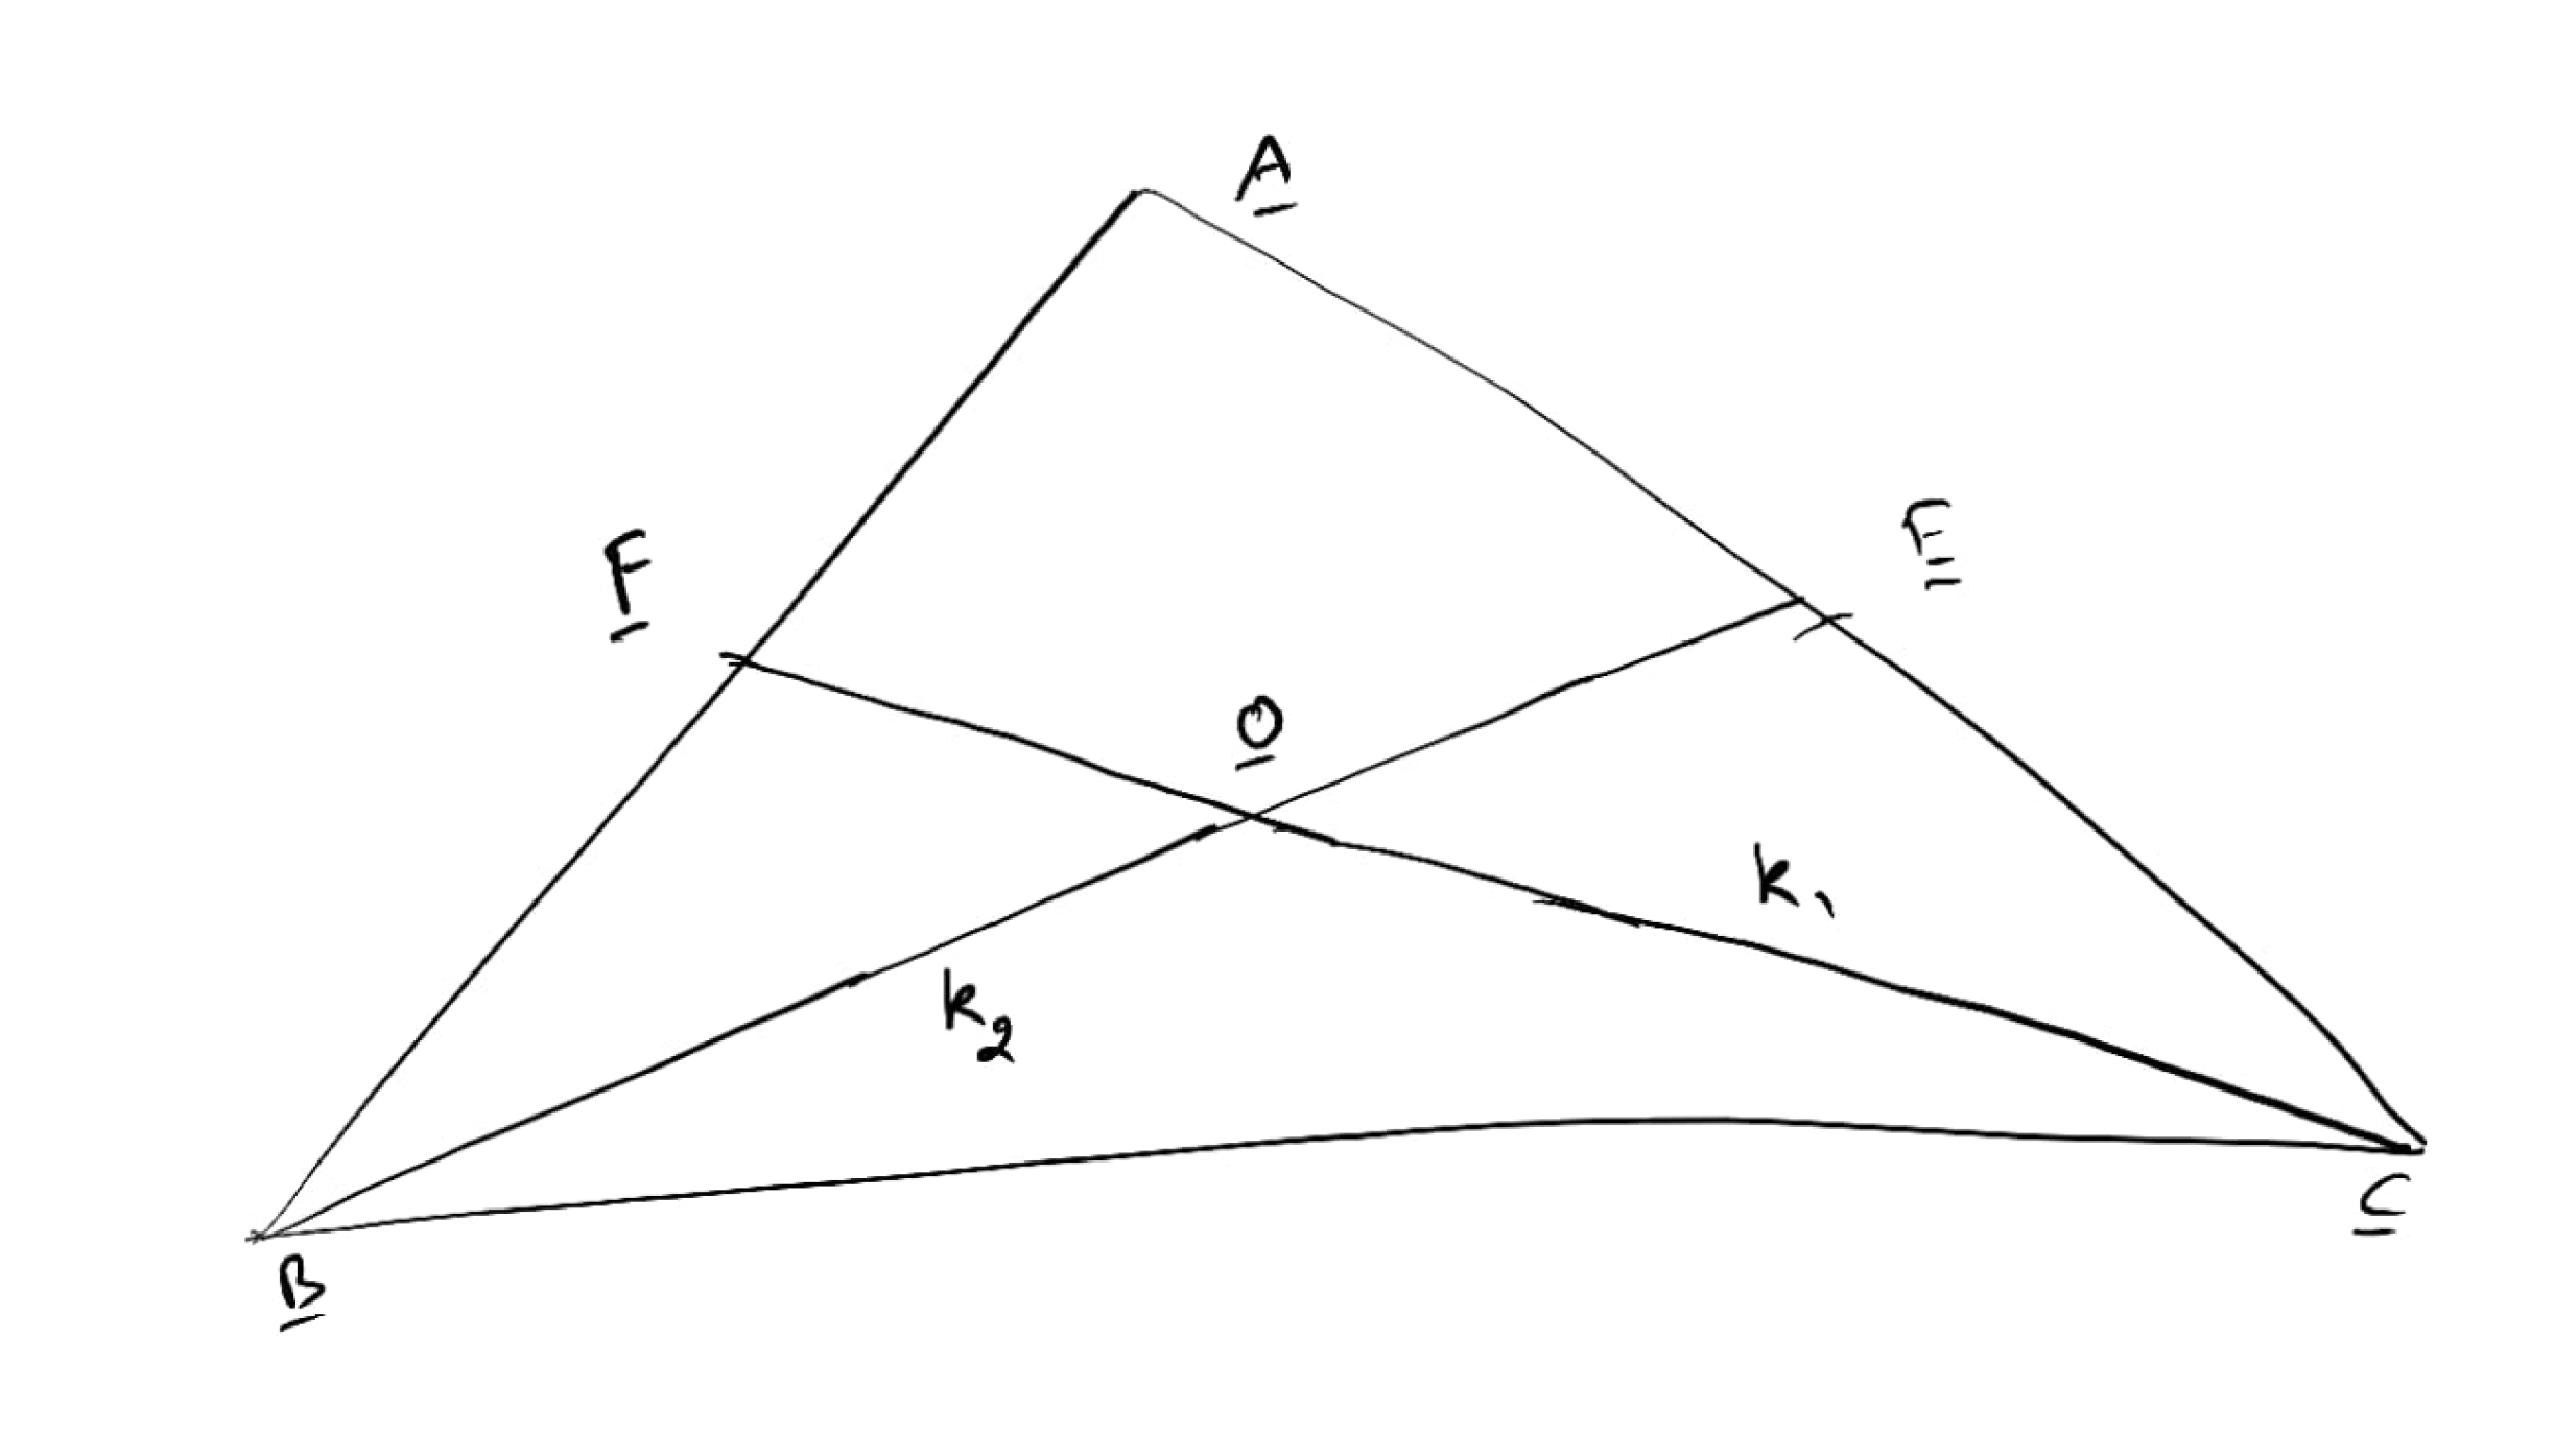
\includegraphics[width=\columnwidth]{./figs/median.eps}
\caption{}
\label{fig:median}
\end{figure}
 Let
\begin{align}
\frac{CO}{OF} &= k_1
\\
\frac{BO}{OE} &= k_2
\end{align}
%
Using  \eqref{eq:ratio},
\begin{align}
\vec{E}&= \frac{\vec{A} + \vec{C}}{2}
\\
\vec{F}&= \frac{\vec{A} + \vec{B}}{2}
\end{align}
%
and
\begin{align}
\label{eq:o1}
\vec{O}&= \frac{k_1\vec{F} + \vec{C}}{k_1+1} = \frac{k_1\frac{\vec{A} + \vec{B}}{2} + \vec{C}}{k_1+1}
\\
\vec{O}&= \frac{k_2\vec{E} + \vec{B}}{k_2+1} = \frac{k_2\frac{\vec{A} + \vec{C}}{2} + \vec{B}}{k_2+1}
\label{eq:o2}
\end{align}
%
From \eqref{eq:o1} and \eqref{eq:o2},
\begin{align}
 \frac{k_1\frac{\vec{A} + \vec{B}}{2} + \vec{C}}{k_1+1} &= 
 \frac{k_2\frac{\vec{A} + \vec{C}}{2} + \vec{B}}{k_2+1}
\end{align}
\begin{multline}
\label{eq:lin_comb}
\implies \sbrak{\frac{k_1\brak{k_2+1}}{2}
-\frac{k_2\brak{k_1+1}}{2}}\vec{A} 
\\
+ 
\sbrak{\frac{k_1\brak{k_2+1}}{2}-\brak{k_1+1}}\vec{B} 
\\
+ \sbrak{\brak{k_2+1}-\frac{k_2\brak{k_1+1}}{2}}\vec{C} 
= 0
\end{multline}
resulting in $k_1 = k_2$,
\begin{align}
k_1^2-k_1-2  &= 0
\implies k_1 = k_2 = 2,
\end{align}
provided $\vec{A},\vec{B},\vec{C}$ are linearly independent. Thus, substituting $k_1=2$ in \eqref{eq:o2},
\begin{equation}
\vec{O} = \frac{\vec{A}+\vec{B}+\vec{C}}{3}
\end{equation}
%
If $\vec{A},\vec{B},\vec{C}$ are linearly dependent,
\begin{align}
\label{eq:lin_dep}
\vec{A} = \alpha \vec{B} + \beta \vec{C} 
\end{align}
%
Note that $\vec{B},\vec{C}$ are linearly independent.
Substituting \eqref{eq:lin_dep} in \eqref{eq:lin_comb},
\begin{multline}
%\label{eq:lin_comb}
 \sbrak{\frac{k_1\brak{k_2+1}}{2}
-\frac{k_2\brak{k_1+1}}{2}}\sbrak{\alpha \vec{B} + \beta \vec{C}  }
\\
+ 
\sbrak{\frac{k_1\brak{k_2+1}}{2}-\brak{k_1+1}}\vec{B} 
\\
+ \sbrak{\brak{k_2+1}-\frac{k_2\brak{k_1+1}}{2}}\vec{C} 
= 0
\end{multline}
\begin{align}
\implies
\begin{split}
\brak{k_1-k_2}\alpha + k_1k_2 - k_1-2 &=0
\\
\brak{k_1-k_2}\beta - k_1k_2 + k_2+2 &=0
\end{split}
\label{eq:median_contra}
\\
\implies \brak{k_1-k_2}\brak{\alpha +\beta - 1} = 0
\end{align}
If $\alpha+\beta = 1, \vec{A},\vec{B},\vec{C}$ are collinear according to \eqref{eq:ratio} resulting in a 
contradiction.  Hence, $k_1=k_2$, which, upon substitution in \eqref{eq:median_contra}, yields
\begin{equation}
k_1^2 - k_1-2 = 0 \implies k_1 = 2.
\end{equation}

\item For what multiples $k, l, m$ is the equation
\begin{align}
k\cbrak{\myvec{2&3}\vec{x}-13}+l\cbrak{\myvec{5& -y}\vec{x}-7} 
\nonumber \\ 
+ m\cbrak{\myvec{1 &-4}\vec{x}+10} = 0
\end{align}
an identity?  In what point do the lines given by equating the three terms to zero concur?
\item Find the equations of the diagonals of the parallelogram
\begin{align}
\myvec{2&-1} \vec{x}+7&= 0
\\
\myvec{ 2 &-1}\vec{x}-5 &= 0,
\\
\myvec{ 3 &2}\vec{x}-5 &= 0
\\
\myvec{ 3 &2}\vec{x}+4&=0 
\end{align}
\renewcommand{\theequation}{\theenumi}
\item The vertices of a triangle are at the points
\begin{align}
\myvec{2\\3}, \myvec{4\\-3}, \myvec{-2\\1}
\end{align}
Find the equations of the perpendiculars to the sides through their middle points.
\numberwithin{equation}{enumi}
\item Work the same problem when the vertices of the triangle are at the points
\begin{align}
\vec{A},
\vec{B},
\vec{C}
\end{align}
and show that the perpendiculars meet in a point.
\\%
\solution In Fig. \ref{fig:alt}, $BE \perp AC, CF \perp AB$.  We need to show that $AD \perp BC$.
\begin{figure}[!hb]
\centering
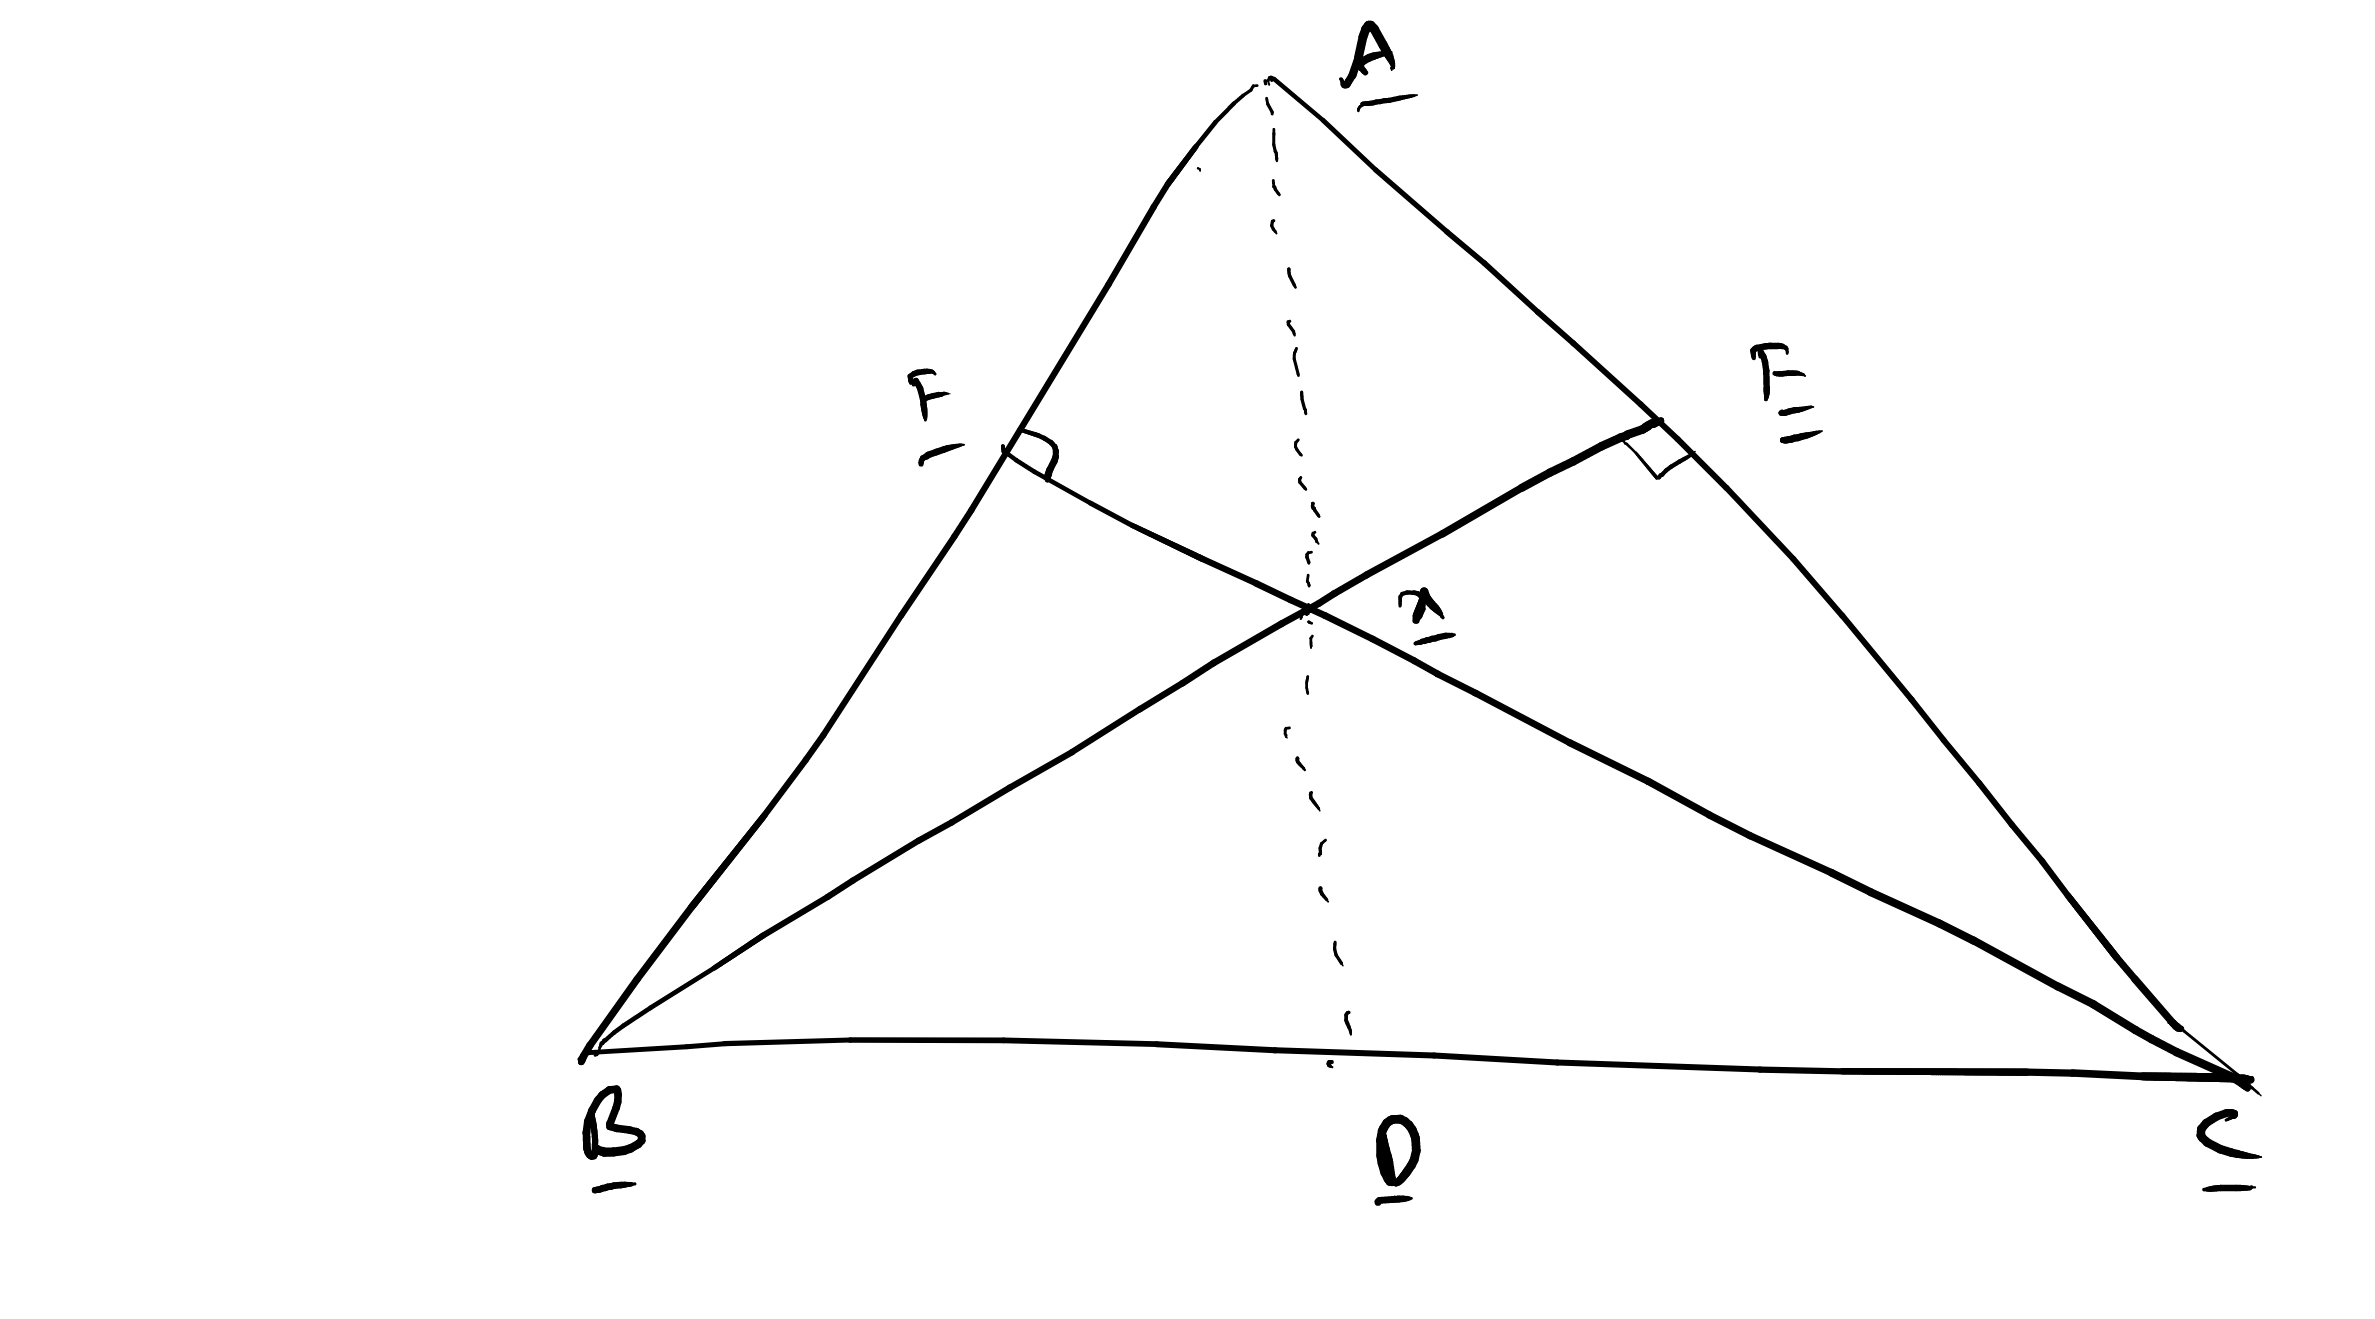
\includegraphics[width=\columnwidth]{./figs/alt.eps}
\caption{}
\label{fig:alt}
\end{figure}
 Let $\vec{x}$ be the intersection of $BE$ and $CF$. Then, using 
\eqref{eq:orth_any},
\begin{align}
\label{eq:alt_1}
\begin{split}
\brak{\vec{x}-\vec{B}}^T
\brak{\vec{A}-\vec{C}} &= 0
\\
\brak{\vec{x}-\vec{C}}^T
\brak{\vec{A}-\vec{B}} &=0
\end{split}
\\
\label{eq:alt_3}
\implies \vec{x}^T\brak{\vec{A}-\vec{C}}-\vec{B}^T\brak{\vec{A}-\vec{C}} &= 0
\\
\text{and }\vec{x}^T\brak{\vec{A}-\vec{B}}-\vec{C}^T\brak{\vec{A}-\vec{B}} &= 0
\label{eq:alt_4}
\end{align}
%
Subtracting \eqref{eq:alt_4} from \eqref{eq:alt_3},
\begin{align}
\vec{x}^T\brak{\vec{B}-\vec{C}} + \vec{A}^T\brak{\vec{C}-\vec{B}} &= 0
\\
\implies \brak{\vec{x}^T - \vec{A}^T}\brak{\vec{B}-\vec{C}}  &= 0
\\
\implies \brak{\vec{x} - \vec{A}}^T\brak{\vec{B}-\vec{C}}  &= 0
\end{align}
%
which completes the proof.
\renewcommand{\theequation}{\theenumi}

\item The line
\begin{align}
\myvec{2 &-8}\vec{x}-4=0
\end{align}
is the perpendicular bisector of the line $AB$ and $\vec{A}$ is the point $\myvec{5\\6}$. What are the coordinates of $\vec{B}$?
\end{enumerate}
 
\subsection{Angle Between Lines}
\renewcommand{\theequation}{\theenumi}
\begin{enumerate}[label=\arabic*.,ref=\thesubsection.\theenumi]
\item What lines are represented by the following equations:
\begin{multicols}{2}
\begin{enumerate}
%{\footnotesize
\item 
$
\vec{x}^T
\myvec{0 & 1\\1 & 0}
\vec{x} = 0
$
\item 
$
\vec{x}^T
\myvec{1 & 0\\0 & -1}
\vec{x} = 0
$
\item 
$
\vec{x}^T
\myvec{6 & \frac{1}{2}\\\frac{1}{2} & -1}
\vec{x} = 0
$
\item 
$
\vec{x}^T
\myvec{-1 & -\tan\theta\\\-\tan\theta & 1}
\vec{x} = 0
$
\item 
$
x^3+3x^2y-3xy^2-y^3 = 0
$
%}
\end{enumerate}
\end{multicols}
\item Find the angles between the pairs of straight lines represented by the following equations:
\begin{multicols}{2}
\begin{enumerate}
\item
$
\vec{x}^T
\myvec{1 & -2\\\-2 & 1}
\vec{x} = 0
$
\item
$
\vec{x}^T
\myvec{1 & 0\\0 & -1}
\vec{x} = 0
$
\item
$
\vec{x}^T
\myvec{1 & -\frac{5}{2}\\-\frac{5}{2} & 4}
\vec{x} = 0
$
\item
$
\vec{x}^T
\myvec{1 & 2\\2 & 0}
\vec{x} = 0
$
\item
$
\vec{x}^T
\myvec{1 & \frac{1}{2}\\ \frac{1}{2} & -6}
\vec{x} = 0
$
\end{enumerate}
\end{multicols}
\numberwithin{equation}{enumi}
\item Prove that the equations
\begin{align}
\vec{x}^T
\myvec{1 & -2\\-2 & 1}
\vec{x} = 0
\\
\myvec{1 & 1}\vec{x} = 3
\end{align}
are the sides of an equilateral triangle.
\end{enumerate}
 
\subsection{Miscellaneous}
\renewcommand{\theequation}{\theenumi}
\begin{enumerate}[label=\arabic*.,ref=\thesubsection.\theenumi]
\item Find the locus of a point which is equidistant from the points $\myvec{6\\-3}$, $\myvec{-4\\7}$.
\item Find the point on the line
\begin{align}
\myvec{2 & 5}\vec{x}+7=0
\end{align}
which is equidistant from the points $\myvec{2\\-3}$, $\myvec{-4\\1}$.
\item Find the coordinates of the circumcentre of the triangle whose corners are at the points $\myvec{4\\3}$, $\myvec{-1\\2}$, $\myvec{2\\-2}$.
\item Find the equations of the lines through $\myvec{3\\1}$ which are respectively parallel and perpendicular to the line joining the points $\myvec{2\\4}$, $\myvec{5\\-6}$.
\item Find the locus of a point at which the join of the points $\myvec{2\\1}$ and $\myvec{-3\\4}$ subtends a right angle.
\item Find the orthocentre of a triangle whose corners are at the points $\myvec{1\\2}$, $\myvec{-3\\-4}$, $\myvec{6\\2}$.
\item Prove that the line joining the points $\myvec{2\\-1}$, $\myvec{-3\\5}$ makes with the axes a triangle of area $\frac{49}{60}$.
\item $ABCD$ is a parallelogram and the coordinates of $\vec{A}$, $\vec{B}$ and $\vec{C}$ are $\myvec{2\\4}$, $\myvec{1\\2}$ and $\myvec{4\\1}$ Find the coordinates of $\vec{D}$.
\item Find the area of the triangle formed by the lines 
\numberwithin{equation}{enumi}
\begin{align}
\myvec{3&-2}\vec{x}=5
\\ 
\myvec{3 &4}\vec{x}=7
\\
\myvec{0 & 1}\vec{x}  +2 = 0
\end{align}
\item Find the centre of the inscribed circle of the triangle whose sides are
\begin{align}
\myvec{3&-4}\vec{x}&=0
\\
\myvec{ 12&-5}\vec{x}&=0,
\\ 
\myvec{4&3}\vec{x}&=8
\end{align}
\renewcommand{\theequation}{\theenumi}
\item The ends of a diagonal of a square are on the coordinate axes at the points $\myvec{2a\\0}$, $\myvec{0\\a}$.  Find the equations of the sides.
\item The sides of a triangle $ABC$ are
\begin{align}
AB=3, BC = 5, CA = 4
\end{align}
and $\vec{A}, \vec{B}$ are on the axes $OX$, $OY$ respectively, while $AC$ makes an angle $\theta$ with $OX$.  Prove that the locus of $\vec{C}$, as $\theta$ varies, is given by the equation
\begin{align}
\vec{x}^T\myvec{16 & -12\\-12 & 25}\vec{x} = 256
%16x^2-24xy+25y^2 = 256
\end{align}
\item Prove that the locus of a point at which the join of the points $\myvec{a\\0}$ and $\myvec{-a\\0}$ subtends an angle of $45\degree$ is
\begin{align}
\vec{x}^T\vec{x}-2a\myvec{0 & 1}\vec{x} = a^2
%x^2+y^2-2ay = a^2
\end{align}
\numberwithin{equation}{enumi}
\item Prove that the line
\begin{align}
\vec{n}^T\vec{x}+c=0
\end{align}
divides the line joining  the points $\vec{x}_1, \vec{x}_2$ in the ratio
\begin{align}
-\frac{\vec{n}^T\vec{x}_1+c}{\vec{n}^T\vec{x}_2+c}
\end{align}
\item Find the equation of the line joining the point $\vec{x}_1$, to the point of intersection of the lines
\begin{align}
\vec{n}^T\vec{x}+c=0
\\
\vec{n}_1^T\vec{x}+c_1=0
\end{align}
\item Find  the equations of the diagonals of the parallelogram whose sides are
\begin{align}
\vec{n}^T\vec{x}+c&=0
\\
\vec{n}^T\vec{x}+d&=0
\\
\vec{n}_1^T\vec{x}+c_1&=0
\\
\vec{n}_1^T\vec{x}+d_1&=0
\end{align}
%are
%{\small
%\begin{align}
%\brak{c_1-d_1}\brak{ax+by+c}-\brak{c-d}\brak{a_1x+b_1y+c_1} = 0
%\\
%\brak{c_1-d_1}\brak{ax+by+c}+\brak{c-d}\brak{a_1x+b_1y+c_1} = 0
%\\
%\brak{c-d}\brak{c_1-d_1}/\brak{ab_1-a_1b}.
%\end{align}
%}
\renewcommand{\theequation}{\theenumi}
\item Prove that for all values of $k$ the line
\begin{align}
\myvec{2+k &1-2k}\vec{x} + 5 = 0
\end{align}
passes through a fixed point, and find its coordinates.
\item Find the angle between the lines
\begin{align}
\vec{x}^T
\myvec{1 & -\sec \theta\\-\sec\theta & 1} 
\vec{x} = 0
\end{align}
\numberwithin{equation}{enumi}
\item Prove that the pairs of straight lines represented by
\begin{align}
\vec{x}^T
\myvec{1 & \frac{1}{2}\\\frac{1}{2} & 0} 
\vec{x} = 0
\\
\vec{x}^T
\myvec{6 & -\frac{1}{2}\\-\frac{1}{2} & -1} 
\vec{x} = 0
\end{align}
are such that the angles between one pair are equal to the angles between the other pair.
\renewcommand{\theequation}{\theenumi}
\item Find the angles between the lines
\begin{align}
x^3-3x^2y-3xy^2+y^3 = 0
\end{align}
\numberwithin{equation}{enumi}
\item Find the area of the triangle whose sides are given by
\begin{align}
\vec{x}^T
\myvec{1 & -{2}\\-{2} & 3} 
\vec{x} = 0
\\
\myvec{3&4}\vec{x}=7
\end{align}
\renewcommand{\theequation}{\theenumi}
\item Show that the equation 
\begin{align}
    \vec{x}^T\myvec{6&-\frac{1}{2}\\-\frac{1}{2}&-15}\vec{x}+\myvec{-11& 31}\vec{x}-10=0\label{eq:solutions/2/6/22/eq:1}
\end{align}
represents two straight lines,and find the equations of the bisectors of the angles between them.
%
%\item Show that the equation
%\begin{align}
%\vec{x}^T
%\myvec{6 & -\frac{1}{2}\\-\frac{1}{2} & -15} 
%\vec{x} 
%+\myvec{-11&31}\vec{x}-10=0
%\end{align}
%represents two straight lines, and find the equations of the bisectors of the angles between them.
\\
\solution
Let the balanced version of (\ref{eq:solutions/chem/6ato balance}) be
\begin{align}
    \label{eq:solutions/chem/6abalanced}x_{1}HNO_{3}+ x_{2}Ca(OH)_{2}\to x_{3}Ca(NO_{3})_{2}+ x_{4}H_{2}O
\end{align}

which results in the following equations:
\begin{align}
    (x_{1}+ 2x_{2}-2x_{4}) H= 0\\
    (x_{1}-2x_{3}) N= 0\\
    (3x_{1}+ 2x_{2}-6x_{3}- x_{4}) O=0\\
    (x_{2}-x_{3}) Ca= 0
\end{align}

which can be expressed as
\begin{align}
    x_{1}+ 2x_{2}+ 0.x_{3} -2x_{4} = 0\\
    x_{1}+ 0.x_{2} -2x_{3} +0.x_{4}= 0\\
    3x_{1}+ 2x_{2}-6x_{3}- x_{4} =0\\
    0.x_{1} +x_{2}-x_{3} +0.x_{4}= 0
\end{align}

resulting in the matrix equation
\begin{align}
    \label{eq:solutions/chem/6a matrix}
    \myvec{1 & 2 & 0 & -2\\
           1 & 0 & -2 & 0\\
           3 & 2 & -6 & -1\\
           0 & 1 & -1 & 0}\vec{x}
           =\vec{0}
\end{align}

where,
\begin{align}
   \vec{x}= \myvec{x_{1}\\x_{2}\\x_{3}\\x_{4}}
\end{align}

(\ref{eq:solutions/chem/6a matrix}) can be reduced as follows:
\begin{align}
    \myvec{1 & 2 & 0 & -2\\
           1 & 0 & -2 & 0\\
           3 & 2 & -6 & -1\\
           0 & 1 & -1 & 0}
    \xleftrightarrow[R_{3}\leftarrow \frac{R_3}{3}-R_{1}]{R_{2}\leftarrow R_2- R_1}
    \myvec{1 & 2 & 0 & -2\\
           0 & -2 & -2 & 2\\
           0 & -\frac{4}{3} & -2 & \frac{5}{3}\\
           0 & 1 & -1 & 0}\\
    \xleftrightarrow{R_2 \leftarrow -\frac{R_2}{2}}
    \myvec{1 & 2 & 0 & -2\\
          0 & 1 & 1 & -1\\
          0 & -\frac{4}{3} & -2 & \frac{5}{3}\\
          0 & 1 & -1 & 0}\\
    \xleftrightarrow[R_4 \leftarrow R_4- R_2]{R_3 \leftarrow R_3 + \frac{4}{3}R_2}
    \myvec{1 & 2 & 0 & -2\\
           0 & 1 & 1 & -1\\
           0 & 0 & -\frac{2}{3} & \frac{1}{3}\\
           0 & 0 & -2 & 1}\\
    \xleftrightarrow[R_3 \leftarrow -\frac{3}{2}R_3]{R_1 \leftarrow R_1- 2R_2}
    \myvec{1 & 0 & -2 & 0\\
           0 & 1 & 1 & -1\\
           0 & 0 & 1 & -\frac{1}{2}\\
           0 & 0 & -2 & 1}\\
    \xleftrightarrow{R_4\leftarrow R_4 + 2R_3}
    \myvec{1 & 0 & -2 & 0\\
           0 & 1 & 1 & -1\\
           0 & 0 & 1 & -\frac{1}{2}\\
           0 & 0 & 0 & 0}\\
    \xleftrightarrow[R_2\leftarrow R_2-R_3]{R_1\leftarrow R_1 + 2R_3}
    \myvec{1 & 0 & 0 & -1\\
           0 & 1 & 0 & -\frac{1}{2}\\
           0 & 0 & 1 & -\frac{1}{2}\\
           0 & 0 & 0 & 0}
\end{align}

Thus,
\begin{align}
    x_1=x_4, x_2= \frac{1}{2}x_4, x_3=\frac{1}{2}x_4\\
    \implies \quad\vec{x}= x_4\myvec{1\\ \frac{1}{2}\\ \frac{1}{2}\\1} =\myvec{2\\1\\1\\2}
\end{align} 
by substituting $x_4= 2$.

\hfill\break
%\vspace{5mm} 
Hence, (\ref{eq:solutions/chem/6abalanced}) finally becomes
\begin{align}
    2HNO_{3}+ Ca(OH)_{2}\to Ca(NO_{3})_{2}+ 2H_{2}O
\end{align}

\item For what value of $k$ does the equation
\begin{align}
\vec{x}^T
\myvec{12 & \frac{7}{2}\\\frac{7}{2} & k} 
\vec{x} 
+\myvec{13&-1}\vec{x}+3=0
\end{align}
represent two straight lines? What is the angle between them?

\item For what value of $k$ does the equation 
\begin{equation} \label{eq:solutions/2/6/24/eq:1.1}
\vec{x}^T \myvec{6 && k/2 \\ k/2 && -3} \vec{x} + \myvec{4 && 5}\vec{x} -2 = 0
\end{equation}
represent a pair of straight lines?
\\
%\item For what values of $k$ does the equation
%\begin{align}
%\vec{x}^T
%\myvec{6 & \frac{k}{2}\\\frac{k}{2} & -3} 
%\vec{x} 
%+\myvec{4&5}\vec{x}-2=0
%\end{align}
%represent two straight lines?
\solution
Let the balanced version of (\ref{eq:solutions/chem/6ato balance}) be
\begin{align}
    \label{eq:solutions/chem/6abalanced}x_{1}HNO_{3}+ x_{2}Ca(OH)_{2}\to x_{3}Ca(NO_{3})_{2}+ x_{4}H_{2}O
\end{align}

which results in the following equations:
\begin{align}
    (x_{1}+ 2x_{2}-2x_{4}) H= 0\\
    (x_{1}-2x_{3}) N= 0\\
    (3x_{1}+ 2x_{2}-6x_{3}- x_{4}) O=0\\
    (x_{2}-x_{3}) Ca= 0
\end{align}

which can be expressed as
\begin{align}
    x_{1}+ 2x_{2}+ 0.x_{3} -2x_{4} = 0\\
    x_{1}+ 0.x_{2} -2x_{3} +0.x_{4}= 0\\
    3x_{1}+ 2x_{2}-6x_{3}- x_{4} =0\\
    0.x_{1} +x_{2}-x_{3} +0.x_{4}= 0
\end{align}

resulting in the matrix equation
\begin{align}
    \label{eq:solutions/chem/6a matrix}
    \myvec{1 & 2 & 0 & -2\\
           1 & 0 & -2 & 0\\
           3 & 2 & -6 & -1\\
           0 & 1 & -1 & 0}\vec{x}
           =\vec{0}
\end{align}

where,
\begin{align}
   \vec{x}= \myvec{x_{1}\\x_{2}\\x_{3}\\x_{4}}
\end{align}

(\ref{eq:solutions/chem/6a matrix}) can be reduced as follows:
\begin{align}
    \myvec{1 & 2 & 0 & -2\\
           1 & 0 & -2 & 0\\
           3 & 2 & -6 & -1\\
           0 & 1 & -1 & 0}
    \xleftrightarrow[R_{3}\leftarrow \frac{R_3}{3}-R_{1}]{R_{2}\leftarrow R_2- R_1}
    \myvec{1 & 2 & 0 & -2\\
           0 & -2 & -2 & 2\\
           0 & -\frac{4}{3} & -2 & \frac{5}{3}\\
           0 & 1 & -1 & 0}\\
    \xleftrightarrow{R_2 \leftarrow -\frac{R_2}{2}}
    \myvec{1 & 2 & 0 & -2\\
          0 & 1 & 1 & -1\\
          0 & -\frac{4}{3} & -2 & \frac{5}{3}\\
          0 & 1 & -1 & 0}\\
    \xleftrightarrow[R_4 \leftarrow R_4- R_2]{R_3 \leftarrow R_3 + \frac{4}{3}R_2}
    \myvec{1 & 2 & 0 & -2\\
           0 & 1 & 1 & -1\\
           0 & 0 & -\frac{2}{3} & \frac{1}{3}\\
           0 & 0 & -2 & 1}\\
    \xleftrightarrow[R_3 \leftarrow -\frac{3}{2}R_3]{R_1 \leftarrow R_1- 2R_2}
    \myvec{1 & 0 & -2 & 0\\
           0 & 1 & 1 & -1\\
           0 & 0 & 1 & -\frac{1}{2}\\
           0 & 0 & -2 & 1}\\
    \xleftrightarrow{R_4\leftarrow R_4 + 2R_3}
    \myvec{1 & 0 & -2 & 0\\
           0 & 1 & 1 & -1\\
           0 & 0 & 1 & -\frac{1}{2}\\
           0 & 0 & 0 & 0}\\
    \xleftrightarrow[R_2\leftarrow R_2-R_3]{R_1\leftarrow R_1 + 2R_3}
    \myvec{1 & 0 & 0 & -1\\
           0 & 1 & 0 & -\frac{1}{2}\\
           0 & 0 & 1 & -\frac{1}{2}\\
           0 & 0 & 0 & 0}
\end{align}

Thus,
\begin{align}
    x_1=x_4, x_2= \frac{1}{2}x_4, x_3=\frac{1}{2}x_4\\
    \implies \quad\vec{x}= x_4\myvec{1\\ \frac{1}{2}\\ \frac{1}{2}\\1} =\myvec{2\\1\\1\\2}
\end{align} 
by substituting $x_4= 2$.

\hfill\break
%\vspace{5mm} 
Hence, (\ref{eq:solutions/chem/6abalanced}) finally becomes
\begin{align}
    2HNO_{3}+ Ca(OH)_{2}\to Ca(NO_{3})_{2}+ 2H_{2}O
\end{align}

%
\end{enumerate}
 
%\newpage
\section{Curves}
\subsection{Properties}
\renewcommand{\theequation}{\theenumi}
\begin{enumerate}[label=\arabic*.,ref=\thesubsection.\theenumi]
\item The equation of a quadratic curve is given by
%\begin{equation}
%Ax_1^2+Bx_1x_2+Cx_2^2+Dx_1+Ex_2+F = 0
%\label{eq:quadratic}
%\end{equation}
%
%Show that  \eqref{eq:quadratic} can be expressed as
\begin{equation}
\vec{x}^T\vec{V}\vec{x}+2\vec{u}^T\vec{x}+ f = 0
\label{eq:quadratic_vec}
\end{equation}
%
%Find the matrix $\vec{V}$ and vector $\vec{u}$.
\item Show that 
\begin{align}
\frac{d\brak{\vec{u}^T\vec{x}}}{d\vec{x}} = \vec{u}
%+ \frac{d\vec{x}}{dx_1}V^T
%= 0
\end{align}
\item Show that 
\begin{align}
\frac{d\brak{\vec{x}^T\vec{V}\vec{x}}}{d\vec{x}} = 2\vec{V}^T\vec{x}
\end{align}
\item Show that 
\begin{align}
\frac{d\vec{x}}{dx_1} = \vec{m}
\end{align}
%
\numberwithin{equation}{enumi}
\item Find the {\em normal} vector to the curve in \eqref{eq:quadratic_vec} at 
point $\vec{p}$.
\\
\solution Differentiating \eqref{eq:quadratic_vec} with respect to 
$x_1$,
\begin{align}
\frac{d\brak{\vec{x}^T\vec{V}\vec{x}}}{d\vec{x}}\frac{d\vec{x}}{dx_1}+\frac{d\brak{\vec{u}^T\vec{x}}}{d\vec{x}}\frac{d\vec{x}}{dx_1}
&= 0
\\
\implies 2\vec{x}^T\vec{V}\vec{m}+2\vec{u}^T\vec{m}
& = 0  \because \brak{\frac{d\vec{x}}{dx_1} = \vec{m}}
\end{align}
Substituting  $\vec{x} = \vec{p}$ and simplifying
\begin{align}
\brak{ \vec{V}\vec{p}+\vec{u}}^T\vec{m} & = 0 
\\
\implies \vec{n} &= \vec{V}\vec{p}+\vec{u}
\end{align}
%
\renewcommand{\theequation}{\theenumi}
\item The {\em tangent} to the curve at $\vec{p}$ is given by 
\begin{align}
\vec{n}^T\brak{\vec{x}-\vec{p}} = 0
\end{align}
%\item Show that the tangent to \eqref{eq:quadratic} at a point $\vec{p}$ on 
%the curve is given by
%\begin{equation}
%\myvec{\vec{p}^T & 1}\myvec{V & \vec{u} \\ \vec{u}^T & F} \myvec{\vec{x} \\ 1} = 0
%\label{eq:tangent_one}
%\end{equation}
%
%Show that \eqref{eq:tangent_one} can be expressed as
This results in
\begin{equation}
\brak{\vec{p}^T\vec{V}+\vec{u}^T}\vec{x} + \vec{p}^T\vec{u} +f = 0
\label{eq:tangent}
\end{equation}

\item Let $\vec{P}$ be a rotation matrix and  $\vec{c}$ be a vector. Then 
\begin{align}
\vec{x} = \vec{P}\vec{y}+\vec{c}.
\label{eq:affine}
\end{align}
 is known as an {\em affine} transformation.
\item Classify the various conic sections based on $\eqref{eq:quadratic_vec}$.
\\
\solution 
\begin{table}[!ht]
\begin{center}
\renewcommand{\theequation}{\theenumi}
%\begin{enumerate}[label=\arabic*.,ref=\theenumi]
\begin{enumerate}[label=\thesection.\arabic*.,ref=\thesection.\theenumi]
\numberwithin{equation}{enumi}

\item Find the area of the region enclosed between the two circles: $\vec{x}^T\vec{x} = 4$ and $\norm{\vec{x}-\myvec{2\\0}} = 2$.
\\
\solution 
Let the balanced version of (\ref{eq:solutions/chem/6ato balance}) be
\begin{align}
    \label{eq:solutions/chem/6abalanced}x_{1}HNO_{3}+ x_{2}Ca(OH)_{2}\to x_{3}Ca(NO_{3})_{2}+ x_{4}H_{2}O
\end{align}

which results in the following equations:
\begin{align}
    (x_{1}+ 2x_{2}-2x_{4}) H= 0\\
    (x_{1}-2x_{3}) N= 0\\
    (3x_{1}+ 2x_{2}-6x_{3}- x_{4}) O=0\\
    (x_{2}-x_{3}) Ca= 0
\end{align}

which can be expressed as
\begin{align}
    x_{1}+ 2x_{2}+ 0.x_{3} -2x_{4} = 0\\
    x_{1}+ 0.x_{2} -2x_{3} +0.x_{4}= 0\\
    3x_{1}+ 2x_{2}-6x_{3}- x_{4} =0\\
    0.x_{1} +x_{2}-x_{3} +0.x_{4}= 0
\end{align}

resulting in the matrix equation
\begin{align}
    \label{eq:solutions/chem/6a matrix}
    \myvec{1 & 2 & 0 & -2\\
           1 & 0 & -2 & 0\\
           3 & 2 & -6 & -1\\
           0 & 1 & -1 & 0}\vec{x}
           =\vec{0}
\end{align}

where,
\begin{align}
   \vec{x}= \myvec{x_{1}\\x_{2}\\x_{3}\\x_{4}}
\end{align}

(\ref{eq:solutions/chem/6a matrix}) can be reduced as follows:
\begin{align}
    \myvec{1 & 2 & 0 & -2\\
           1 & 0 & -2 & 0\\
           3 & 2 & -6 & -1\\
           0 & 1 & -1 & 0}
    \xleftrightarrow[R_{3}\leftarrow \frac{R_3}{3}-R_{1}]{R_{2}\leftarrow R_2- R_1}
    \myvec{1 & 2 & 0 & -2\\
           0 & -2 & -2 & 2\\
           0 & -\frac{4}{3} & -2 & \frac{5}{3}\\
           0 & 1 & -1 & 0}\\
    \xleftrightarrow{R_2 \leftarrow -\frac{R_2}{2}}
    \myvec{1 & 2 & 0 & -2\\
          0 & 1 & 1 & -1\\
          0 & -\frac{4}{3} & -2 & \frac{5}{3}\\
          0 & 1 & -1 & 0}\\
    \xleftrightarrow[R_4 \leftarrow R_4- R_2]{R_3 \leftarrow R_3 + \frac{4}{3}R_2}
    \myvec{1 & 2 & 0 & -2\\
           0 & 1 & 1 & -1\\
           0 & 0 & -\frac{2}{3} & \frac{1}{3}\\
           0 & 0 & -2 & 1}\\
    \xleftrightarrow[R_3 \leftarrow -\frac{3}{2}R_3]{R_1 \leftarrow R_1- 2R_2}
    \myvec{1 & 0 & -2 & 0\\
           0 & 1 & 1 & -1\\
           0 & 0 & 1 & -\frac{1}{2}\\
           0 & 0 & -2 & 1}\\
    \xleftrightarrow{R_4\leftarrow R_4 + 2R_3}
    \myvec{1 & 0 & -2 & 0\\
           0 & 1 & 1 & -1\\
           0 & 0 & 1 & -\frac{1}{2}\\
           0 & 0 & 0 & 0}\\
    \xleftrightarrow[R_2\leftarrow R_2-R_3]{R_1\leftarrow R_1 + 2R_3}
    \myvec{1 & 0 & 0 & -1\\
           0 & 1 & 0 & -\frac{1}{2}\\
           0 & 0 & 1 & -\frac{1}{2}\\
           0 & 0 & 0 & 0}
\end{align}

Thus,
\begin{align}
    x_1=x_4, x_2= \frac{1}{2}x_4, x_3=\frac{1}{2}x_4\\
    \implies \quad\vec{x}= x_4\myvec{1\\ \frac{1}{2}\\ \frac{1}{2}\\1} =\myvec{2\\1\\1\\2}
\end{align} 
by substituting $x_4= 2$.

\hfill\break
%\vspace{5mm} 
Hence, (\ref{eq:solutions/chem/6abalanced}) finally becomes
\begin{align}
    2HNO_{3}+ Ca(OH)_{2}\to Ca(NO_{3})_{2}+ 2H_{2}O
\end{align}

\item Find the equation of the circle with radius 5 whose centre lies on x-axis and passes through the point \myvec{2\\3}.
\\
\solution 
Let the balanced version of (\ref{eq:solutions/chem/6ato balance}) be
\begin{align}
    \label{eq:solutions/chem/6abalanced}x_{1}HNO_{3}+ x_{2}Ca(OH)_{2}\to x_{3}Ca(NO_{3})_{2}+ x_{4}H_{2}O
\end{align}

which results in the following equations:
\begin{align}
    (x_{1}+ 2x_{2}-2x_{4}) H= 0\\
    (x_{1}-2x_{3}) N= 0\\
    (3x_{1}+ 2x_{2}-6x_{3}- x_{4}) O=0\\
    (x_{2}-x_{3}) Ca= 0
\end{align}

which can be expressed as
\begin{align}
    x_{1}+ 2x_{2}+ 0.x_{3} -2x_{4} = 0\\
    x_{1}+ 0.x_{2} -2x_{3} +0.x_{4}= 0\\
    3x_{1}+ 2x_{2}-6x_{3}- x_{4} =0\\
    0.x_{1} +x_{2}-x_{3} +0.x_{4}= 0
\end{align}

resulting in the matrix equation
\begin{align}
    \label{eq:solutions/chem/6a matrix}
    \myvec{1 & 2 & 0 & -2\\
           1 & 0 & -2 & 0\\
           3 & 2 & -6 & -1\\
           0 & 1 & -1 & 0}\vec{x}
           =\vec{0}
\end{align}

where,
\begin{align}
   \vec{x}= \myvec{x_{1}\\x_{2}\\x_{3}\\x_{4}}
\end{align}

(\ref{eq:solutions/chem/6a matrix}) can be reduced as follows:
\begin{align}
    \myvec{1 & 2 & 0 & -2\\
           1 & 0 & -2 & 0\\
           3 & 2 & -6 & -1\\
           0 & 1 & -1 & 0}
    \xleftrightarrow[R_{3}\leftarrow \frac{R_3}{3}-R_{1}]{R_{2}\leftarrow R_2- R_1}
    \myvec{1 & 2 & 0 & -2\\
           0 & -2 & -2 & 2\\
           0 & -\frac{4}{3} & -2 & \frac{5}{3}\\
           0 & 1 & -1 & 0}\\
    \xleftrightarrow{R_2 \leftarrow -\frac{R_2}{2}}
    \myvec{1 & 2 & 0 & -2\\
          0 & 1 & 1 & -1\\
          0 & -\frac{4}{3} & -2 & \frac{5}{3}\\
          0 & 1 & -1 & 0}\\
    \xleftrightarrow[R_4 \leftarrow R_4- R_2]{R_3 \leftarrow R_3 + \frac{4}{3}R_2}
    \myvec{1 & 2 & 0 & -2\\
           0 & 1 & 1 & -1\\
           0 & 0 & -\frac{2}{3} & \frac{1}{3}\\
           0 & 0 & -2 & 1}\\
    \xleftrightarrow[R_3 \leftarrow -\frac{3}{2}R_3]{R_1 \leftarrow R_1- 2R_2}
    \myvec{1 & 0 & -2 & 0\\
           0 & 1 & 1 & -1\\
           0 & 0 & 1 & -\frac{1}{2}\\
           0 & 0 & -2 & 1}\\
    \xleftrightarrow{R_4\leftarrow R_4 + 2R_3}
    \myvec{1 & 0 & -2 & 0\\
           0 & 1 & 1 & -1\\
           0 & 0 & 1 & -\frac{1}{2}\\
           0 & 0 & 0 & 0}\\
    \xleftrightarrow[R_2\leftarrow R_2-R_3]{R_1\leftarrow R_1 + 2R_3}
    \myvec{1 & 0 & 0 & -1\\
           0 & 1 & 0 & -\frac{1}{2}\\
           0 & 0 & 1 & -\frac{1}{2}\\
           0 & 0 & 0 & 0}
\end{align}

Thus,
\begin{align}
    x_1=x_4, x_2= \frac{1}{2}x_4, x_3=\frac{1}{2}x_4\\
    \implies \quad\vec{x}= x_4\myvec{1\\ \frac{1}{2}\\ \frac{1}{2}\\1} =\myvec{2\\1\\1\\2}
\end{align} 
by substituting $x_4= 2$.

\hfill\break
%\vspace{5mm} 
Hence, (\ref{eq:solutions/chem/6abalanced}) finally becomes
\begin{align}
    2HNO_{3}+ Ca(OH)_{2}\to Ca(NO_{3})_{2}+ 2H_{2}O
\end{align}

\item Find the equation of the circle passing through \myvec{0\\0} and making intercepts a and b on the coordinate axes.
\item Find the equation of a circle with centre \myvec{2\\2} and passes through the point \myvec{4\\5}. 
\\
\solution 
Let the balanced version of (\ref{eq:solutions/chem/6ato balance}) be
\begin{align}
    \label{eq:solutions/chem/6abalanced}x_{1}HNO_{3}+ x_{2}Ca(OH)_{2}\to x_{3}Ca(NO_{3})_{2}+ x_{4}H_{2}O
\end{align}

which results in the following equations:
\begin{align}
    (x_{1}+ 2x_{2}-2x_{4}) H= 0\\
    (x_{1}-2x_{3}) N= 0\\
    (3x_{1}+ 2x_{2}-6x_{3}- x_{4}) O=0\\
    (x_{2}-x_{3}) Ca= 0
\end{align}

which can be expressed as
\begin{align}
    x_{1}+ 2x_{2}+ 0.x_{3} -2x_{4} = 0\\
    x_{1}+ 0.x_{2} -2x_{3} +0.x_{4}= 0\\
    3x_{1}+ 2x_{2}-6x_{3}- x_{4} =0\\
    0.x_{1} +x_{2}-x_{3} +0.x_{4}= 0
\end{align}

resulting in the matrix equation
\begin{align}
    \label{eq:solutions/chem/6a matrix}
    \myvec{1 & 2 & 0 & -2\\
           1 & 0 & -2 & 0\\
           3 & 2 & -6 & -1\\
           0 & 1 & -1 & 0}\vec{x}
           =\vec{0}
\end{align}

where,
\begin{align}
   \vec{x}= \myvec{x_{1}\\x_{2}\\x_{3}\\x_{4}}
\end{align}

(\ref{eq:solutions/chem/6a matrix}) can be reduced as follows:
\begin{align}
    \myvec{1 & 2 & 0 & -2\\
           1 & 0 & -2 & 0\\
           3 & 2 & -6 & -1\\
           0 & 1 & -1 & 0}
    \xleftrightarrow[R_{3}\leftarrow \frac{R_3}{3}-R_{1}]{R_{2}\leftarrow R_2- R_1}
    \myvec{1 & 2 & 0 & -2\\
           0 & -2 & -2 & 2\\
           0 & -\frac{4}{3} & -2 & \frac{5}{3}\\
           0 & 1 & -1 & 0}\\
    \xleftrightarrow{R_2 \leftarrow -\frac{R_2}{2}}
    \myvec{1 & 2 & 0 & -2\\
          0 & 1 & 1 & -1\\
          0 & -\frac{4}{3} & -2 & \frac{5}{3}\\
          0 & 1 & -1 & 0}\\
    \xleftrightarrow[R_4 \leftarrow R_4- R_2]{R_3 \leftarrow R_3 + \frac{4}{3}R_2}
    \myvec{1 & 2 & 0 & -2\\
           0 & 1 & 1 & -1\\
           0 & 0 & -\frac{2}{3} & \frac{1}{3}\\
           0 & 0 & -2 & 1}\\
    \xleftrightarrow[R_3 \leftarrow -\frac{3}{2}R_3]{R_1 \leftarrow R_1- 2R_2}
    \myvec{1 & 0 & -2 & 0\\
           0 & 1 & 1 & -1\\
           0 & 0 & 1 & -\frac{1}{2}\\
           0 & 0 & -2 & 1}\\
    \xleftrightarrow{R_4\leftarrow R_4 + 2R_3}
    \myvec{1 & 0 & -2 & 0\\
           0 & 1 & 1 & -1\\
           0 & 0 & 1 & -\frac{1}{2}\\
           0 & 0 & 0 & 0}\\
    \xleftrightarrow[R_2\leftarrow R_2-R_3]{R_1\leftarrow R_1 + 2R_3}
    \myvec{1 & 0 & 0 & -1\\
           0 & 1 & 0 & -\frac{1}{2}\\
           0 & 0 & 1 & -\frac{1}{2}\\
           0 & 0 & 0 & 0}
\end{align}

Thus,
\begin{align}
    x_1=x_4, x_2= \frac{1}{2}x_4, x_3=\frac{1}{2}x_4\\
    \implies \quad\vec{x}= x_4\myvec{1\\ \frac{1}{2}\\ \frac{1}{2}\\1} =\myvec{2\\1\\1\\2}
\end{align} 
by substituting $x_4= 2$.

\hfill\break
%\vspace{5mm} 
Hence, (\ref{eq:solutions/chem/6abalanced}) finally becomes
\begin{align}
    2HNO_{3}+ Ca(OH)_{2}\to Ca(NO_{3})_{2}+ 2H_{2}O
\end{align}

\item Find the locus of all the unit vectors in the xy-plane.
%
\item Find the points on the curve $\vec{x}^T\vec{x}-2\myvec{1 & 0}\vec{x} -3 =0$  at which the tangents are parallel to the x-axis.
%
\\
\solution
Let the balanced version of (\ref{eq:solutions/chem/6ato balance}) be
\begin{align}
    \label{eq:solutions/chem/6abalanced}x_{1}HNO_{3}+ x_{2}Ca(OH)_{2}\to x_{3}Ca(NO_{3})_{2}+ x_{4}H_{2}O
\end{align}

which results in the following equations:
\begin{align}
    (x_{1}+ 2x_{2}-2x_{4}) H= 0\\
    (x_{1}-2x_{3}) N= 0\\
    (3x_{1}+ 2x_{2}-6x_{3}- x_{4}) O=0\\
    (x_{2}-x_{3}) Ca= 0
\end{align}

which can be expressed as
\begin{align}
    x_{1}+ 2x_{2}+ 0.x_{3} -2x_{4} = 0\\
    x_{1}+ 0.x_{2} -2x_{3} +0.x_{4}= 0\\
    3x_{1}+ 2x_{2}-6x_{3}- x_{4} =0\\
    0.x_{1} +x_{2}-x_{3} +0.x_{4}= 0
\end{align}

resulting in the matrix equation
\begin{align}
    \label{eq:solutions/chem/6a matrix}
    \myvec{1 & 2 & 0 & -2\\
           1 & 0 & -2 & 0\\
           3 & 2 & -6 & -1\\
           0 & 1 & -1 & 0}\vec{x}
           =\vec{0}
\end{align}

where,
\begin{align}
   \vec{x}= \myvec{x_{1}\\x_{2}\\x_{3}\\x_{4}}
\end{align}

(\ref{eq:solutions/chem/6a matrix}) can be reduced as follows:
\begin{align}
    \myvec{1 & 2 & 0 & -2\\
           1 & 0 & -2 & 0\\
           3 & 2 & -6 & -1\\
           0 & 1 & -1 & 0}
    \xleftrightarrow[R_{3}\leftarrow \frac{R_3}{3}-R_{1}]{R_{2}\leftarrow R_2- R_1}
    \myvec{1 & 2 & 0 & -2\\
           0 & -2 & -2 & 2\\
           0 & -\frac{4}{3} & -2 & \frac{5}{3}\\
           0 & 1 & -1 & 0}\\
    \xleftrightarrow{R_2 \leftarrow -\frac{R_2}{2}}
    \myvec{1 & 2 & 0 & -2\\
          0 & 1 & 1 & -1\\
          0 & -\frac{4}{3} & -2 & \frac{5}{3}\\
          0 & 1 & -1 & 0}\\
    \xleftrightarrow[R_4 \leftarrow R_4- R_2]{R_3 \leftarrow R_3 + \frac{4}{3}R_2}
    \myvec{1 & 2 & 0 & -2\\
           0 & 1 & 1 & -1\\
           0 & 0 & -\frac{2}{3} & \frac{1}{3}\\
           0 & 0 & -2 & 1}\\
    \xleftrightarrow[R_3 \leftarrow -\frac{3}{2}R_3]{R_1 \leftarrow R_1- 2R_2}
    \myvec{1 & 0 & -2 & 0\\
           0 & 1 & 1 & -1\\
           0 & 0 & 1 & -\frac{1}{2}\\
           0 & 0 & -2 & 1}\\
    \xleftrightarrow{R_4\leftarrow R_4 + 2R_3}
    \myvec{1 & 0 & -2 & 0\\
           0 & 1 & 1 & -1\\
           0 & 0 & 1 & -\frac{1}{2}\\
           0 & 0 & 0 & 0}\\
    \xleftrightarrow[R_2\leftarrow R_2-R_3]{R_1\leftarrow R_1 + 2R_3}
    \myvec{1 & 0 & 0 & -1\\
           0 & 1 & 0 & -\frac{1}{2}\\
           0 & 0 & 1 & -\frac{1}{2}\\
           0 & 0 & 0 & 0}
\end{align}

Thus,
\begin{align}
    x_1=x_4, x_2= \frac{1}{2}x_4, x_3=\frac{1}{2}x_4\\
    \implies \quad\vec{x}= x_4\myvec{1\\ \frac{1}{2}\\ \frac{1}{2}\\1} =\myvec{2\\1\\1\\2}
\end{align} 
by substituting $x_4= 2$.

\hfill\break
%\vspace{5mm} 
Hence, (\ref{eq:solutions/chem/6abalanced}) finally becomes
\begin{align}
    2HNO_{3}+ Ca(OH)_{2}\to Ca(NO_{3})_{2}+ 2H_{2}O
\end{align}

\item  Find the area of the region in the first quadrant enclosed by x-axis, line $\myvec{1 & -\sqrt{3}}\vec{x} =0$ and the circle $\vec{x}^T\vec{x}=4$.
%
\\
\solution
Let the balanced version of (\ref{eq:solutions/chem/6ato balance}) be
\begin{align}
    \label{eq:solutions/chem/6abalanced}x_{1}HNO_{3}+ x_{2}Ca(OH)_{2}\to x_{3}Ca(NO_{3})_{2}+ x_{4}H_{2}O
\end{align}

which results in the following equations:
\begin{align}
    (x_{1}+ 2x_{2}-2x_{4}) H= 0\\
    (x_{1}-2x_{3}) N= 0\\
    (3x_{1}+ 2x_{2}-6x_{3}- x_{4}) O=0\\
    (x_{2}-x_{3}) Ca= 0
\end{align}

which can be expressed as
\begin{align}
    x_{1}+ 2x_{2}+ 0.x_{3} -2x_{4} = 0\\
    x_{1}+ 0.x_{2} -2x_{3} +0.x_{4}= 0\\
    3x_{1}+ 2x_{2}-6x_{3}- x_{4} =0\\
    0.x_{1} +x_{2}-x_{3} +0.x_{4}= 0
\end{align}

resulting in the matrix equation
\begin{align}
    \label{eq:solutions/chem/6a matrix}
    \myvec{1 & 2 & 0 & -2\\
           1 & 0 & -2 & 0\\
           3 & 2 & -6 & -1\\
           0 & 1 & -1 & 0}\vec{x}
           =\vec{0}
\end{align}

where,
\begin{align}
   \vec{x}= \myvec{x_{1}\\x_{2}\\x_{3}\\x_{4}}
\end{align}

(\ref{eq:solutions/chem/6a matrix}) can be reduced as follows:
\begin{align}
    \myvec{1 & 2 & 0 & -2\\
           1 & 0 & -2 & 0\\
           3 & 2 & -6 & -1\\
           0 & 1 & -1 & 0}
    \xleftrightarrow[R_{3}\leftarrow \frac{R_3}{3}-R_{1}]{R_{2}\leftarrow R_2- R_1}
    \myvec{1 & 2 & 0 & -2\\
           0 & -2 & -2 & 2\\
           0 & -\frac{4}{3} & -2 & \frac{5}{3}\\
           0 & 1 & -1 & 0}\\
    \xleftrightarrow{R_2 \leftarrow -\frac{R_2}{2}}
    \myvec{1 & 2 & 0 & -2\\
          0 & 1 & 1 & -1\\
          0 & -\frac{4}{3} & -2 & \frac{5}{3}\\
          0 & 1 & -1 & 0}\\
    \xleftrightarrow[R_4 \leftarrow R_4- R_2]{R_3 \leftarrow R_3 + \frac{4}{3}R_2}
    \myvec{1 & 2 & 0 & -2\\
           0 & 1 & 1 & -1\\
           0 & 0 & -\frac{2}{3} & \frac{1}{3}\\
           0 & 0 & -2 & 1}\\
    \xleftrightarrow[R_3 \leftarrow -\frac{3}{2}R_3]{R_1 \leftarrow R_1- 2R_2}
    \myvec{1 & 0 & -2 & 0\\
           0 & 1 & 1 & -1\\
           0 & 0 & 1 & -\frac{1}{2}\\
           0 & 0 & -2 & 1}\\
    \xleftrightarrow{R_4\leftarrow R_4 + 2R_3}
    \myvec{1 & 0 & -2 & 0\\
           0 & 1 & 1 & -1\\
           0 & 0 & 1 & -\frac{1}{2}\\
           0 & 0 & 0 & 0}\\
    \xleftrightarrow[R_2\leftarrow R_2-R_3]{R_1\leftarrow R_1 + 2R_3}
    \myvec{1 & 0 & 0 & -1\\
           0 & 1 & 0 & -\frac{1}{2}\\
           0 & 0 & 1 & -\frac{1}{2}\\
           0 & 0 & 0 & 0}
\end{align}

Thus,
\begin{align}
    x_1=x_4, x_2= \frac{1}{2}x_4, x_3=\frac{1}{2}x_4\\
    \implies \quad\vec{x}= x_4\myvec{1\\ \frac{1}{2}\\ \frac{1}{2}\\1} =\myvec{2\\1\\1\\2}
\end{align} 
by substituting $x_4= 2$.

\hfill\break
%\vspace{5mm} 
Hence, (\ref{eq:solutions/chem/6abalanced}) finally becomes
\begin{align}
    2HNO_{3}+ Ca(OH)_{2}\to Ca(NO_{3})_{2}+ 2H_{2}O
\end{align}

\item Find the area lying in the first quadrant and bounded by the circle $\vec{x}^T\vec{x}=4$ and the lines $x = 0$ and $x = 2$.
%
\item Find the area of the circle $4\vec{x}^T\vec{x}=9$.
\item  Find the area bounded by curves $\norm{\vec{x}-\myvec{1\\0}} = 1$ and $\norm{\vec{x}}=1$
\\
\solution
Let the balanced version of (\ref{eq:solutions/chem/6ato balance}) be
\begin{align}
    \label{eq:solutions/chem/6abalanced}x_{1}HNO_{3}+ x_{2}Ca(OH)_{2}\to x_{3}Ca(NO_{3})_{2}+ x_{4}H_{2}O
\end{align}

which results in the following equations:
\begin{align}
    (x_{1}+ 2x_{2}-2x_{4}) H= 0\\
    (x_{1}-2x_{3}) N= 0\\
    (3x_{1}+ 2x_{2}-6x_{3}- x_{4}) O=0\\
    (x_{2}-x_{3}) Ca= 0
\end{align}

which can be expressed as
\begin{align}
    x_{1}+ 2x_{2}+ 0.x_{3} -2x_{4} = 0\\
    x_{1}+ 0.x_{2} -2x_{3} +0.x_{4}= 0\\
    3x_{1}+ 2x_{2}-6x_{3}- x_{4} =0\\
    0.x_{1} +x_{2}-x_{3} +0.x_{4}= 0
\end{align}

resulting in the matrix equation
\begin{align}
    \label{eq:solutions/chem/6a matrix}
    \myvec{1 & 2 & 0 & -2\\
           1 & 0 & -2 & 0\\
           3 & 2 & -6 & -1\\
           0 & 1 & -1 & 0}\vec{x}
           =\vec{0}
\end{align}

where,
\begin{align}
   \vec{x}= \myvec{x_{1}\\x_{2}\\x_{3}\\x_{4}}
\end{align}

(\ref{eq:solutions/chem/6a matrix}) can be reduced as follows:
\begin{align}
    \myvec{1 & 2 & 0 & -2\\
           1 & 0 & -2 & 0\\
           3 & 2 & -6 & -1\\
           0 & 1 & -1 & 0}
    \xleftrightarrow[R_{3}\leftarrow \frac{R_3}{3}-R_{1}]{R_{2}\leftarrow R_2- R_1}
    \myvec{1 & 2 & 0 & -2\\
           0 & -2 & -2 & 2\\
           0 & -\frac{4}{3} & -2 & \frac{5}{3}\\
           0 & 1 & -1 & 0}\\
    \xleftrightarrow{R_2 \leftarrow -\frac{R_2}{2}}
    \myvec{1 & 2 & 0 & -2\\
          0 & 1 & 1 & -1\\
          0 & -\frac{4}{3} & -2 & \frac{5}{3}\\
          0 & 1 & -1 & 0}\\
    \xleftrightarrow[R_4 \leftarrow R_4- R_2]{R_3 \leftarrow R_3 + \frac{4}{3}R_2}
    \myvec{1 & 2 & 0 & -2\\
           0 & 1 & 1 & -1\\
           0 & 0 & -\frac{2}{3} & \frac{1}{3}\\
           0 & 0 & -2 & 1}\\
    \xleftrightarrow[R_3 \leftarrow -\frac{3}{2}R_3]{R_1 \leftarrow R_1- 2R_2}
    \myvec{1 & 0 & -2 & 0\\
           0 & 1 & 1 & -1\\
           0 & 0 & 1 & -\frac{1}{2}\\
           0 & 0 & -2 & 1}\\
    \xleftrightarrow{R_4\leftarrow R_4 + 2R_3}
    \myvec{1 & 0 & -2 & 0\\
           0 & 1 & 1 & -1\\
           0 & 0 & 1 & -\frac{1}{2}\\
           0 & 0 & 0 & 0}\\
    \xleftrightarrow[R_2\leftarrow R_2-R_3]{R_1\leftarrow R_1 + 2R_3}
    \myvec{1 & 0 & 0 & -1\\
           0 & 1 & 0 & -\frac{1}{2}\\
           0 & 0 & 1 & -\frac{1}{2}\\
           0 & 0 & 0 & 0}
\end{align}

Thus,
\begin{align}
    x_1=x_4, x_2= \frac{1}{2}x_4, x_3=\frac{1}{2}x_4\\
    \implies \quad\vec{x}= x_4\myvec{1\\ \frac{1}{2}\\ \frac{1}{2}\\1} =\myvec{2\\1\\1\\2}
\end{align} 
by substituting $x_4= 2$.

\hfill\break
%\vspace{5mm} 
Hence, (\ref{eq:solutions/chem/6abalanced}) finally becomes
\begin{align}
    2HNO_{3}+ Ca(OH)_{2}\to Ca(NO_{3})_{2}+ 2H_{2}O
\end{align}

\item Find the smaller area enclosed by the circle $\vec{x}^T\vec{x}=4$ and the line $\myvec{1 & 1}\vec{x} = 2$.


\item Find the slope of the tangent to the curve $y = \frac{x-1}{x-2}, x\ne 2$ at $x = 10$.
\\
\solution
Let the balanced version of (\ref{eq:solutions/chem/6ato balance}) be
\begin{align}
    \label{eq:solutions/chem/6abalanced}x_{1}HNO_{3}+ x_{2}Ca(OH)_{2}\to x_{3}Ca(NO_{3})_{2}+ x_{4}H_{2}O
\end{align}

which results in the following equations:
\begin{align}
    (x_{1}+ 2x_{2}-2x_{4}) H= 0\\
    (x_{1}-2x_{3}) N= 0\\
    (3x_{1}+ 2x_{2}-6x_{3}- x_{4}) O=0\\
    (x_{2}-x_{3}) Ca= 0
\end{align}

which can be expressed as
\begin{align}
    x_{1}+ 2x_{2}+ 0.x_{3} -2x_{4} = 0\\
    x_{1}+ 0.x_{2} -2x_{3} +0.x_{4}= 0\\
    3x_{1}+ 2x_{2}-6x_{3}- x_{4} =0\\
    0.x_{1} +x_{2}-x_{3} +0.x_{4}= 0
\end{align}

resulting in the matrix equation
\begin{align}
    \label{eq:solutions/chem/6a matrix}
    \myvec{1 & 2 & 0 & -2\\
           1 & 0 & -2 & 0\\
           3 & 2 & -6 & -1\\
           0 & 1 & -1 & 0}\vec{x}
           =\vec{0}
\end{align}

where,
\begin{align}
   \vec{x}= \myvec{x_{1}\\x_{2}\\x_{3}\\x_{4}}
\end{align}

(\ref{eq:solutions/chem/6a matrix}) can be reduced as follows:
\begin{align}
    \myvec{1 & 2 & 0 & -2\\
           1 & 0 & -2 & 0\\
           3 & 2 & -6 & -1\\
           0 & 1 & -1 & 0}
    \xleftrightarrow[R_{3}\leftarrow \frac{R_3}{3}-R_{1}]{R_{2}\leftarrow R_2- R_1}
    \myvec{1 & 2 & 0 & -2\\
           0 & -2 & -2 & 2\\
           0 & -\frac{4}{3} & -2 & \frac{5}{3}\\
           0 & 1 & -1 & 0}\\
    \xleftrightarrow{R_2 \leftarrow -\frac{R_2}{2}}
    \myvec{1 & 2 & 0 & -2\\
          0 & 1 & 1 & -1\\
          0 & -\frac{4}{3} & -2 & \frac{5}{3}\\
          0 & 1 & -1 & 0}\\
    \xleftrightarrow[R_4 \leftarrow R_4- R_2]{R_3 \leftarrow R_3 + \frac{4}{3}R_2}
    \myvec{1 & 2 & 0 & -2\\
           0 & 1 & 1 & -1\\
           0 & 0 & -\frac{2}{3} & \frac{1}{3}\\
           0 & 0 & -2 & 1}\\
    \xleftrightarrow[R_3 \leftarrow -\frac{3}{2}R_3]{R_1 \leftarrow R_1- 2R_2}
    \myvec{1 & 0 & -2 & 0\\
           0 & 1 & 1 & -1\\
           0 & 0 & 1 & -\frac{1}{2}\\
           0 & 0 & -2 & 1}\\
    \xleftrightarrow{R_4\leftarrow R_4 + 2R_3}
    \myvec{1 & 0 & -2 & 0\\
           0 & 1 & 1 & -1\\
           0 & 0 & 1 & -\frac{1}{2}\\
           0 & 0 & 0 & 0}\\
    \xleftrightarrow[R_2\leftarrow R_2-R_3]{R_1\leftarrow R_1 + 2R_3}
    \myvec{1 & 0 & 0 & -1\\
           0 & 1 & 0 & -\frac{1}{2}\\
           0 & 0 & 1 & -\frac{1}{2}\\
           0 & 0 & 0 & 0}
\end{align}

Thus,
\begin{align}
    x_1=x_4, x_2= \frac{1}{2}x_4, x_3=\frac{1}{2}x_4\\
    \implies \quad\vec{x}= x_4\myvec{1\\ \frac{1}{2}\\ \frac{1}{2}\\1} =\myvec{2\\1\\1\\2}
\end{align} 
by substituting $x_4= 2$.

\hfill\break
%\vspace{5mm} 
Hence, (\ref{eq:solutions/chem/6abalanced}) finally becomes
\begin{align}
    2HNO_{3}+ Ca(OH)_{2}\to Ca(NO_{3})_{2}+ 2H_{2}O
\end{align}

\item Find a point on the curve $y = (x – 2)^2$ at which the tangent is parallel to the chord joining the points \myvec{2\\ 0} and \myvec{4\\ 4}.
\\
\solution
Let the balanced version of (\ref{eq:solutions/chem/6ato balance}) be
\begin{align}
    \label{eq:solutions/chem/6abalanced}x_{1}HNO_{3}+ x_{2}Ca(OH)_{2}\to x_{3}Ca(NO_{3})_{2}+ x_{4}H_{2}O
\end{align}

which results in the following equations:
\begin{align}
    (x_{1}+ 2x_{2}-2x_{4}) H= 0\\
    (x_{1}-2x_{3}) N= 0\\
    (3x_{1}+ 2x_{2}-6x_{3}- x_{4}) O=0\\
    (x_{2}-x_{3}) Ca= 0
\end{align}

which can be expressed as
\begin{align}
    x_{1}+ 2x_{2}+ 0.x_{3} -2x_{4} = 0\\
    x_{1}+ 0.x_{2} -2x_{3} +0.x_{4}= 0\\
    3x_{1}+ 2x_{2}-6x_{3}- x_{4} =0\\
    0.x_{1} +x_{2}-x_{3} +0.x_{4}= 0
\end{align}

resulting in the matrix equation
\begin{align}
    \label{eq:solutions/chem/6a matrix}
    \myvec{1 & 2 & 0 & -2\\
           1 & 0 & -2 & 0\\
           3 & 2 & -6 & -1\\
           0 & 1 & -1 & 0}\vec{x}
           =\vec{0}
\end{align}

where,
\begin{align}
   \vec{x}= \myvec{x_{1}\\x_{2}\\x_{3}\\x_{4}}
\end{align}

(\ref{eq:solutions/chem/6a matrix}) can be reduced as follows:
\begin{align}
    \myvec{1 & 2 & 0 & -2\\
           1 & 0 & -2 & 0\\
           3 & 2 & -6 & -1\\
           0 & 1 & -1 & 0}
    \xleftrightarrow[R_{3}\leftarrow \frac{R_3}{3}-R_{1}]{R_{2}\leftarrow R_2- R_1}
    \myvec{1 & 2 & 0 & -2\\
           0 & -2 & -2 & 2\\
           0 & -\frac{4}{3} & -2 & \frac{5}{3}\\
           0 & 1 & -1 & 0}\\
    \xleftrightarrow{R_2 \leftarrow -\frac{R_2}{2}}
    \myvec{1 & 2 & 0 & -2\\
          0 & 1 & 1 & -1\\
          0 & -\frac{4}{3} & -2 & \frac{5}{3}\\
          0 & 1 & -1 & 0}\\
    \xleftrightarrow[R_4 \leftarrow R_4- R_2]{R_3 \leftarrow R_3 + \frac{4}{3}R_2}
    \myvec{1 & 2 & 0 & -2\\
           0 & 1 & 1 & -1\\
           0 & 0 & -\frac{2}{3} & \frac{1}{3}\\
           0 & 0 & -2 & 1}\\
    \xleftrightarrow[R_3 \leftarrow -\frac{3}{2}R_3]{R_1 \leftarrow R_1- 2R_2}
    \myvec{1 & 0 & -2 & 0\\
           0 & 1 & 1 & -1\\
           0 & 0 & 1 & -\frac{1}{2}\\
           0 & 0 & -2 & 1}\\
    \xleftrightarrow{R_4\leftarrow R_4 + 2R_3}
    \myvec{1 & 0 & -2 & 0\\
           0 & 1 & 1 & -1\\
           0 & 0 & 1 & -\frac{1}{2}\\
           0 & 0 & 0 & 0}\\
    \xleftrightarrow[R_2\leftarrow R_2-R_3]{R_1\leftarrow R_1 + 2R_3}
    \myvec{1 & 0 & 0 & -1\\
           0 & 1 & 0 & -\frac{1}{2}\\
           0 & 0 & 1 & -\frac{1}{2}\\
           0 & 0 & 0 & 0}
\end{align}

Thus,
\begin{align}
    x_1=x_4, x_2= \frac{1}{2}x_4, x_3=\frac{1}{2}x_4\\
    \implies \quad\vec{x}= x_4\myvec{1\\ \frac{1}{2}\\ \frac{1}{2}\\1} =\myvec{2\\1\\1\\2}
\end{align} 
by substituting $x_4= 2$.

\hfill\break
%\vspace{5mm} 
Hence, (\ref{eq:solutions/chem/6abalanced}) finally becomes
\begin{align}
    2HNO_{3}+ Ca(OH)_{2}\to Ca(NO_{3})_{2}+ 2H_{2}O
\end{align}

\item Find the equation of all lines having slope – 1 that are tangents to the curve $\frac{1}
{x -1}, x \ne 1$
\\
\solution 
Let the balanced version of (\ref{eq:solutions/chem/6ato balance}) be
\begin{align}
    \label{eq:solutions/chem/6abalanced}x_{1}HNO_{3}+ x_{2}Ca(OH)_{2}\to x_{3}Ca(NO_{3})_{2}+ x_{4}H_{2}O
\end{align}

which results in the following equations:
\begin{align}
    (x_{1}+ 2x_{2}-2x_{4}) H= 0\\
    (x_{1}-2x_{3}) N= 0\\
    (3x_{1}+ 2x_{2}-6x_{3}- x_{4}) O=0\\
    (x_{2}-x_{3}) Ca= 0
\end{align}

which can be expressed as
\begin{align}
    x_{1}+ 2x_{2}+ 0.x_{3} -2x_{4} = 0\\
    x_{1}+ 0.x_{2} -2x_{3} +0.x_{4}= 0\\
    3x_{1}+ 2x_{2}-6x_{3}- x_{4} =0\\
    0.x_{1} +x_{2}-x_{3} +0.x_{4}= 0
\end{align}

resulting in the matrix equation
\begin{align}
    \label{eq:solutions/chem/6a matrix}
    \myvec{1 & 2 & 0 & -2\\
           1 & 0 & -2 & 0\\
           3 & 2 & -6 & -1\\
           0 & 1 & -1 & 0}\vec{x}
           =\vec{0}
\end{align}

where,
\begin{align}
   \vec{x}= \myvec{x_{1}\\x_{2}\\x_{3}\\x_{4}}
\end{align}

(\ref{eq:solutions/chem/6a matrix}) can be reduced as follows:
\begin{align}
    \myvec{1 & 2 & 0 & -2\\
           1 & 0 & -2 & 0\\
           3 & 2 & -6 & -1\\
           0 & 1 & -1 & 0}
    \xleftrightarrow[R_{3}\leftarrow \frac{R_3}{3}-R_{1}]{R_{2}\leftarrow R_2- R_1}
    \myvec{1 & 2 & 0 & -2\\
           0 & -2 & -2 & 2\\
           0 & -\frac{4}{3} & -2 & \frac{5}{3}\\
           0 & 1 & -1 & 0}\\
    \xleftrightarrow{R_2 \leftarrow -\frac{R_2}{2}}
    \myvec{1 & 2 & 0 & -2\\
          0 & 1 & 1 & -1\\
          0 & -\frac{4}{3} & -2 & \frac{5}{3}\\
          0 & 1 & -1 & 0}\\
    \xleftrightarrow[R_4 \leftarrow R_4- R_2]{R_3 \leftarrow R_3 + \frac{4}{3}R_2}
    \myvec{1 & 2 & 0 & -2\\
           0 & 1 & 1 & -1\\
           0 & 0 & -\frac{2}{3} & \frac{1}{3}\\
           0 & 0 & -2 & 1}\\
    \xleftrightarrow[R_3 \leftarrow -\frac{3}{2}R_3]{R_1 \leftarrow R_1- 2R_2}
    \myvec{1 & 0 & -2 & 0\\
           0 & 1 & 1 & -1\\
           0 & 0 & 1 & -\frac{1}{2}\\
           0 & 0 & -2 & 1}\\
    \xleftrightarrow{R_4\leftarrow R_4 + 2R_3}
    \myvec{1 & 0 & -2 & 0\\
           0 & 1 & 1 & -1\\
           0 & 0 & 1 & -\frac{1}{2}\\
           0 & 0 & 0 & 0}\\
    \xleftrightarrow[R_2\leftarrow R_2-R_3]{R_1\leftarrow R_1 + 2R_3}
    \myvec{1 & 0 & 0 & -1\\
           0 & 1 & 0 & -\frac{1}{2}\\
           0 & 0 & 1 & -\frac{1}{2}\\
           0 & 0 & 0 & 0}
\end{align}

Thus,
\begin{align}
    x_1=x_4, x_2= \frac{1}{2}x_4, x_3=\frac{1}{2}x_4\\
    \implies \quad\vec{x}= x_4\myvec{1\\ \frac{1}{2}\\ \frac{1}{2}\\1} =\myvec{2\\1\\1\\2}
\end{align} 
by substituting $x_4= 2$.

\hfill\break
%\vspace{5mm} 
Hence, (\ref{eq:solutions/chem/6abalanced}) finally becomes
\begin{align}
    2HNO_{3}+ Ca(OH)_{2}\to Ca(NO_{3})_{2}+ 2H_{2}O
\end{align}

\item Find the equation of all lines having slope -2 which are tangents to the curve $\frac{1}
{x - 3} , x \ne 3$.
%
\\
\solution 
Let the balanced version of (\ref{eq:solutions/chem/6ato balance}) be
\begin{align}
    \label{eq:solutions/chem/6abalanced}x_{1}HNO_{3}+ x_{2}Ca(OH)_{2}\to x_{3}Ca(NO_{3})_{2}+ x_{4}H_{2}O
\end{align}

which results in the following equations:
\begin{align}
    (x_{1}+ 2x_{2}-2x_{4}) H= 0\\
    (x_{1}-2x_{3}) N= 0\\
    (3x_{1}+ 2x_{2}-6x_{3}- x_{4}) O=0\\
    (x_{2}-x_{3}) Ca= 0
\end{align}

which can be expressed as
\begin{align}
    x_{1}+ 2x_{2}+ 0.x_{3} -2x_{4} = 0\\
    x_{1}+ 0.x_{2} -2x_{3} +0.x_{4}= 0\\
    3x_{1}+ 2x_{2}-6x_{3}- x_{4} =0\\
    0.x_{1} +x_{2}-x_{3} +0.x_{4}= 0
\end{align}

resulting in the matrix equation
\begin{align}
    \label{eq:solutions/chem/6a matrix}
    \myvec{1 & 2 & 0 & -2\\
           1 & 0 & -2 & 0\\
           3 & 2 & -6 & -1\\
           0 & 1 & -1 & 0}\vec{x}
           =\vec{0}
\end{align}

where,
\begin{align}
   \vec{x}= \myvec{x_{1}\\x_{2}\\x_{3}\\x_{4}}
\end{align}

(\ref{eq:solutions/chem/6a matrix}) can be reduced as follows:
\begin{align}
    \myvec{1 & 2 & 0 & -2\\
           1 & 0 & -2 & 0\\
           3 & 2 & -6 & -1\\
           0 & 1 & -1 & 0}
    \xleftrightarrow[R_{3}\leftarrow \frac{R_3}{3}-R_{1}]{R_{2}\leftarrow R_2- R_1}
    \myvec{1 & 2 & 0 & -2\\
           0 & -2 & -2 & 2\\
           0 & -\frac{4}{3} & -2 & \frac{5}{3}\\
           0 & 1 & -1 & 0}\\
    \xleftrightarrow{R_2 \leftarrow -\frac{R_2}{2}}
    \myvec{1 & 2 & 0 & -2\\
          0 & 1 & 1 & -1\\
          0 & -\frac{4}{3} & -2 & \frac{5}{3}\\
          0 & 1 & -1 & 0}\\
    \xleftrightarrow[R_4 \leftarrow R_4- R_2]{R_3 \leftarrow R_3 + \frac{4}{3}R_2}
    \myvec{1 & 2 & 0 & -2\\
           0 & 1 & 1 & -1\\
           0 & 0 & -\frac{2}{3} & \frac{1}{3}\\
           0 & 0 & -2 & 1}\\
    \xleftrightarrow[R_3 \leftarrow -\frac{3}{2}R_3]{R_1 \leftarrow R_1- 2R_2}
    \myvec{1 & 0 & -2 & 0\\
           0 & 1 & 1 & -1\\
           0 & 0 & 1 & -\frac{1}{2}\\
           0 & 0 & -2 & 1}\\
    \xleftrightarrow{R_4\leftarrow R_4 + 2R_3}
    \myvec{1 & 0 & -2 & 0\\
           0 & 1 & 1 & -1\\
           0 & 0 & 1 & -\frac{1}{2}\\
           0 & 0 & 0 & 0}\\
    \xleftrightarrow[R_2\leftarrow R_2-R_3]{R_1\leftarrow R_1 + 2R_3}
    \myvec{1 & 0 & 0 & -1\\
           0 & 1 & 0 & -\frac{1}{2}\\
           0 & 0 & 1 & -\frac{1}{2}\\
           0 & 0 & 0 & 0}
\end{align}

Thus,
\begin{align}
    x_1=x_4, x_2= \frac{1}{2}x_4, x_3=\frac{1}{2}x_4\\
    \implies \quad\vec{x}= x_4\myvec{1\\ \frac{1}{2}\\ \frac{1}{2}\\1} =\myvec{2\\1\\1\\2}
\end{align} 
by substituting $x_4= 2$.

\hfill\break
%\vspace{5mm} 
Hence, (\ref{eq:solutions/chem/6abalanced}) finally becomes
\begin{align}
    2HNO_{3}+ Ca(OH)_{2}\to Ca(NO_{3})_{2}+ 2H_{2}O
\end{align}

\item Find points on the curve 
$
\vec{x}^T\myvec{\frac{1}{9} & 0 \\ 0 & \frac{1}{16}}\vec{x} = 1
$
%
at which tangents are
\begin{enumerate}
\item  parallel to x-axis
\item  parallel to y-axis.
\end{enumerate}
\solution 
Let the balanced version of (\ref{eq:solutions/chem/6ato balance}) be
\begin{align}
    \label{eq:solutions/chem/6abalanced}x_{1}HNO_{3}+ x_{2}Ca(OH)_{2}\to x_{3}Ca(NO_{3})_{2}+ x_{4}H_{2}O
\end{align}

which results in the following equations:
\begin{align}
    (x_{1}+ 2x_{2}-2x_{4}) H= 0\\
    (x_{1}-2x_{3}) N= 0\\
    (3x_{1}+ 2x_{2}-6x_{3}- x_{4}) O=0\\
    (x_{2}-x_{3}) Ca= 0
\end{align}

which can be expressed as
\begin{align}
    x_{1}+ 2x_{2}+ 0.x_{3} -2x_{4} = 0\\
    x_{1}+ 0.x_{2} -2x_{3} +0.x_{4}= 0\\
    3x_{1}+ 2x_{2}-6x_{3}- x_{4} =0\\
    0.x_{1} +x_{2}-x_{3} +0.x_{4}= 0
\end{align}

resulting in the matrix equation
\begin{align}
    \label{eq:solutions/chem/6a matrix}
    \myvec{1 & 2 & 0 & -2\\
           1 & 0 & -2 & 0\\
           3 & 2 & -6 & -1\\
           0 & 1 & -1 & 0}\vec{x}
           =\vec{0}
\end{align}

where,
\begin{align}
   \vec{x}= \myvec{x_{1}\\x_{2}\\x_{3}\\x_{4}}
\end{align}

(\ref{eq:solutions/chem/6a matrix}) can be reduced as follows:
\begin{align}
    \myvec{1 & 2 & 0 & -2\\
           1 & 0 & -2 & 0\\
           3 & 2 & -6 & -1\\
           0 & 1 & -1 & 0}
    \xleftrightarrow[R_{3}\leftarrow \frac{R_3}{3}-R_{1}]{R_{2}\leftarrow R_2- R_1}
    \myvec{1 & 2 & 0 & -2\\
           0 & -2 & -2 & 2\\
           0 & -\frac{4}{3} & -2 & \frac{5}{3}\\
           0 & 1 & -1 & 0}\\
    \xleftrightarrow{R_2 \leftarrow -\frac{R_2}{2}}
    \myvec{1 & 2 & 0 & -2\\
          0 & 1 & 1 & -1\\
          0 & -\frac{4}{3} & -2 & \frac{5}{3}\\
          0 & 1 & -1 & 0}\\
    \xleftrightarrow[R_4 \leftarrow R_4- R_2]{R_3 \leftarrow R_3 + \frac{4}{3}R_2}
    \myvec{1 & 2 & 0 & -2\\
           0 & 1 & 1 & -1\\
           0 & 0 & -\frac{2}{3} & \frac{1}{3}\\
           0 & 0 & -2 & 1}\\
    \xleftrightarrow[R_3 \leftarrow -\frac{3}{2}R_3]{R_1 \leftarrow R_1- 2R_2}
    \myvec{1 & 0 & -2 & 0\\
           0 & 1 & 1 & -1\\
           0 & 0 & 1 & -\frac{1}{2}\\
           0 & 0 & -2 & 1}\\
    \xleftrightarrow{R_4\leftarrow R_4 + 2R_3}
    \myvec{1 & 0 & -2 & 0\\
           0 & 1 & 1 & -1\\
           0 & 0 & 1 & -\frac{1}{2}\\
           0 & 0 & 0 & 0}\\
    \xleftrightarrow[R_2\leftarrow R_2-R_3]{R_1\leftarrow R_1 + 2R_3}
    \myvec{1 & 0 & 0 & -1\\
           0 & 1 & 0 & -\frac{1}{2}\\
           0 & 0 & 1 & -\frac{1}{2}\\
           0 & 0 & 0 & 0}
\end{align}

Thus,
\begin{align}
    x_1=x_4, x_2= \frac{1}{2}x_4, x_3=\frac{1}{2}x_4\\
    \implies \quad\vec{x}= x_4\myvec{1\\ \frac{1}{2}\\ \frac{1}{2}\\1} =\myvec{2\\1\\1\\2}
\end{align} 
by substituting $x_4= 2$.

\hfill\break
%\vspace{5mm} 
Hence, (\ref{eq:solutions/chem/6abalanced}) finally becomes
\begin{align}
    2HNO_{3}+ Ca(OH)_{2}\to Ca(NO_{3})_{2}+ 2H_{2}O
\end{align}

\item Find the equations of the tangent and normal to the given curves at the indicated points:
$
y = x^2
$
at \myvec{0\\0}.
\item Find the equation of the tangent line to the curve $y = x^2-2x+7$
\begin{enumerate}
%
\item  parallel to the line $\myvec{2 & -1}\vec{x}= -9$ 
\item  perpendicular to the line $\myvec{-15 & 5}\vec{x} = 13$. 
\end{enumerate}
\item  Find the equation of the tangent to the curve,
\begin{align}
y = \sqrt{3x-2}
\label{eq:solutions/1/19/Q}
\end{align}
 which is parallel to the line,
\begin{align}
\myvec{4&2}\vec{x}+5=0
\label{eq:solutions/1/19/P}
\end{align}  
\solution 
Let the balanced version of (\ref{eq:solutions/chem/6ato balance}) be
\begin{align}
    \label{eq:solutions/chem/6abalanced}x_{1}HNO_{3}+ x_{2}Ca(OH)_{2}\to x_{3}Ca(NO_{3})_{2}+ x_{4}H_{2}O
\end{align}

which results in the following equations:
\begin{align}
    (x_{1}+ 2x_{2}-2x_{4}) H= 0\\
    (x_{1}-2x_{3}) N= 0\\
    (3x_{1}+ 2x_{2}-6x_{3}- x_{4}) O=0\\
    (x_{2}-x_{3}) Ca= 0
\end{align}

which can be expressed as
\begin{align}
    x_{1}+ 2x_{2}+ 0.x_{3} -2x_{4} = 0\\
    x_{1}+ 0.x_{2} -2x_{3} +0.x_{4}= 0\\
    3x_{1}+ 2x_{2}-6x_{3}- x_{4} =0\\
    0.x_{1} +x_{2}-x_{3} +0.x_{4}= 0
\end{align}

resulting in the matrix equation
\begin{align}
    \label{eq:solutions/chem/6a matrix}
    \myvec{1 & 2 & 0 & -2\\
           1 & 0 & -2 & 0\\
           3 & 2 & -6 & -1\\
           0 & 1 & -1 & 0}\vec{x}
           =\vec{0}
\end{align}

where,
\begin{align}
   \vec{x}= \myvec{x_{1}\\x_{2}\\x_{3}\\x_{4}}
\end{align}

(\ref{eq:solutions/chem/6a matrix}) can be reduced as follows:
\begin{align}
    \myvec{1 & 2 & 0 & -2\\
           1 & 0 & -2 & 0\\
           3 & 2 & -6 & -1\\
           0 & 1 & -1 & 0}
    \xleftrightarrow[R_{3}\leftarrow \frac{R_3}{3}-R_{1}]{R_{2}\leftarrow R_2- R_1}
    \myvec{1 & 2 & 0 & -2\\
           0 & -2 & -2 & 2\\
           0 & -\frac{4}{3} & -2 & \frac{5}{3}\\
           0 & 1 & -1 & 0}\\
    \xleftrightarrow{R_2 \leftarrow -\frac{R_2}{2}}
    \myvec{1 & 2 & 0 & -2\\
          0 & 1 & 1 & -1\\
          0 & -\frac{4}{3} & -2 & \frac{5}{3}\\
          0 & 1 & -1 & 0}\\
    \xleftrightarrow[R_4 \leftarrow R_4- R_2]{R_3 \leftarrow R_3 + \frac{4}{3}R_2}
    \myvec{1 & 2 & 0 & -2\\
           0 & 1 & 1 & -1\\
           0 & 0 & -\frac{2}{3} & \frac{1}{3}\\
           0 & 0 & -2 & 1}\\
    \xleftrightarrow[R_3 \leftarrow -\frac{3}{2}R_3]{R_1 \leftarrow R_1- 2R_2}
    \myvec{1 & 0 & -2 & 0\\
           0 & 1 & 1 & -1\\
           0 & 0 & 1 & -\frac{1}{2}\\
           0 & 0 & -2 & 1}\\
    \xleftrightarrow{R_4\leftarrow R_4 + 2R_3}
    \myvec{1 & 0 & -2 & 0\\
           0 & 1 & 1 & -1\\
           0 & 0 & 1 & -\frac{1}{2}\\
           0 & 0 & 0 & 0}\\
    \xleftrightarrow[R_2\leftarrow R_2-R_3]{R_1\leftarrow R_1 + 2R_3}
    \myvec{1 & 0 & 0 & -1\\
           0 & 1 & 0 & -\frac{1}{2}\\
           0 & 0 & 1 & -\frac{1}{2}\\
           0 & 0 & 0 & 0}
\end{align}

Thus,
\begin{align}
    x_1=x_4, x_2= \frac{1}{2}x_4, x_3=\frac{1}{2}x_4\\
    \implies \quad\vec{x}= x_4\myvec{1\\ \frac{1}{2}\\ \frac{1}{2}\\1} =\myvec{2\\1\\1\\2}
\end{align} 
by substituting $x_4= 2$.

\hfill\break
%\vspace{5mm} 
Hence, (\ref{eq:solutions/chem/6abalanced}) finally becomes
\begin{align}
    2HNO_{3}+ Ca(OH)_{2}\to Ca(NO_{3})_{2}+ 2H_{2}O
\end{align}

%
\item Find the point at which the line $\myvec{-1 & 1}\vec{x} =  1$ is a tangent to the curve $y^2 = 4x$.
%
\item The line $\myvec{-m & 1}\vec{x} = 1$ is a tangent to the curve $y^2 = 4x$.  Find the value of $m$.
\item  Find the normal at the point \myvec{1\\1} on the curve $2y + x^2 = 3$ 
\item  Find the normal to the curve $x^2=4y$ passing through $\myvec{1\\2}$.
%
\item Find the area of the region bounded by the curve $y^2= x$ and the lines $x = 1, x = 4$ and the x-axis in the first quadrant.
\item  Find the area of the region bounded by $y^2=9x, x=2, x=4$ and the x-axis in the  first quadrant.
%
\item Find the area of the region bounded by $x^2 = 4y, y = 2, y = 4$ and the y-axis in the first quadrant.
\item Find the area of the region bounded by the ellipse 
$
\vec{x}^T\myvec{\frac{1}{16} & 0 \\ 0 & \frac{1}{9}}\vec{x} = 1
$

\item  Find the area of the region bounded by the ellipse 
$
\vec{x}^T\myvec{\frac{1}{4} & 0 \\ 0 & \frac{1}{9}}\vec{x} = 1
$
\item The area between $x=y^2$ and $x=4$ is divided into two equal parts by the line $x=a$, find the value of $a$.
\item  Find the area of the region bounded by the parabola $y = x^2$ and $y = \abs{x}$.
\item  Find the area bounded by the curve $x^2 = 4y$ and the line $\myvec{1 & -1}\vec{x} = -2$.
\item  Find the area of the region bounded by the curve $y^2 = 4x$ and the line $x = 3$.
%
\item Find the area of the region bounded by the curve $y^2 = x$, y-axis and the line $y = 3$.
%
\item Find the area of the region bounded by the two parabolas $y = x^2, y^2=x$.
\item Find the area lying above x-axis and included between the circle $\vec{x}^T\vec{x} -8\myvec{1 & 0}= 0$  and inside of the parabola $y^2 = 4x$.
%
\item AOBA is the part of the ellipse 
$
\vec{x}^T\myvec{9 & 0 \\ 0 & 1}\vec{x} = 36
$
in the first quadrant such that $OA = 2$ and $OB = 6$. Find the area between the arc $AB$ and the chord $AB$.
\item Find the area lying between the curves $y^2 = 4x$ and $y = 2x$.
\item  Find the area of the region bounded by the curves $y = x^2+2, y = x, x = 0$ and $ x = 3.$
%
\item Find the area under $y = x^2, x = 1, x = 2$ and x-axis.
\item Find the area between  $y = x^2$ and $y = x$.
\item Find the area of the region lying in the first quadrant and bounded by $y = 4x^2, x = 0, y = 1$ and $y = 4$.
\item Find the area enclosed by the parabola $4y = 3x^2$ and the line $\myvec{-3 & 2}\vec{x} = 12$.
%
\item Find the area of the smaller region bounded by the ellipse
$
\vec{x}^T\myvec{\frac{1}{9} & 0 \\ 0 & \frac{1}{4}}\vec{x} = 1
$
and the line 
$
\myvec{\frac{1}{a} & \frac{1}{b}}\vec{x} = 1
$
\item Find the area of the region enclosed by the parabola $x^2=y$, the line $\myvec{-1 & 1}\vec{x} = 2$ and the x-axis.
%
\item Find the area bounded by the curves
\begin{align}
\cbrak{\brak{x,y} : y > x^2, y = \abs{x}}
\end{align}
%
\item Find the area of the region
\begin{align}
\cbrak{\brak{x,y} : y^2 \le 4x, 4\vec{x}^T\vec{x} = 9}
\end{align}
%
\item Find the area of the circle $\vec{x}^T\vec{x} = 16$ exterior to the parabola $y^2 = 6$.
\end{enumerate}

\end{center}
\caption{}
\label{table:conics}
\end{table}

%\item Show that the tangent to \eqref{eq:quadratic} at a point $\vec{p}$ on 
%the curve is given by
%\begin{equation}
%\myvec{\vec{p}^T & 1}\myvec{V & \vec{u} \\ \vec{u}^T & F} \myvec{\vec{x} \\ 1} = 0
%\label{eq:tangent_one}
%\end{equation}
%%
%\item Show that \eqref{eq:tangent_one} can be expressed as
%\begin{equation}
%\brak{\vec{p}^T\vec{V}+\vec{u}^T}\vec{x} + \vec{p}^T\vec{u} +f = 0
%\label{eq:tangent}
%\end{equation}
\end{enumerate}
 
\subsection{Circle}
\renewcommand{\theequation}{\theenumi}
\begin{enumerate}[label=\arabic*.,ref=\thesubsection.\theenumi]
\numberwithin{equation}{enumi}

\item Find the centre and radius of the circle
\begin{equation}
C_1: \vec{x}^T\vec{x} - \myvec{2 & 0}\vec{x} 
-1 = 0 
\label{eq:circle_c1}
\end{equation}
%
\\
\solution let $\vec{c}$ be the centre of the circle.  Then
\begin{align}
\norm{\vec{x}-\vec{c}}^2 &= r^2
\\
\implies \brak{\vec{x}-\vec{c}}^T\brak{\vec{x}-\vec{c}} &= r^2
\\
\implies \vec{x}^T\vec{x} - 2\vec{c}^T\vec{x} &= r^2-\vec{c}^T\vec{c}
\end{align}
%
Comparing with \eqref{eq:circle_c1},
\begin{align}
\vec{c} &= \myvec{1 \\0}
\\
r^2-\vec{c}^T\vec{c} &= 1 \implies r = \sqrt{2}
\end{align}

\item Find the tangent to the circle $C_1$
at the point $\myvec{2 \\1}$.
\\
\solution From \eqref{eq:tangent}, the tangent $T$ is given by
\begin{align}
\sbrak{\myvec{2 & 1}-\myvec{1 & 0}}\vec{x} -\myvec{2 & 1}\myvec{1 \\ 0}  &= 1
\\
\implies T: \vec{n}^T\vec{x}   &= 3
\label{eq:circle_tangent}
\end{align}
%
where
\begin{equation}
\vec{n}=\myvec{1 \\ 1}
\end{equation}
\item The tangent $T$ in \eqref{eq:circle_tangent} cuts off a chord $AB$
from a circle $C_2$ whose 
centre is 
\begin{equation}
\vec{C}=\myvec{3 \\ 
-2}. 
\end{equation}
Find $\vec{A}+ \vec{B}$.
\\
\solution Let the radius of $C_2$ be $r$.  From the given information,
\begin{align}
\brak{\vec{A}-\vec{C}}^T\brak{ \vec{A}-\vec{C} } &= r^2
\label{eq:circle_x1}
\\
\brak{\vec{B}-\vec{C}}^T\brak{ \vec{B}-\vec{C} } &= r^2
\label{eq:circle_x2}
\end{align}
%
 Subtracting 
\eqref{eq:circle_x2} from \eqref{eq:circle_x1},
\begin{flalign}
&\vec{A}^T \vec{A}-\vec{B}^T \vec{B}-2\vec{C}^T\brak{\vec{A}- \vec{B}}  = 0
\\
&\implies \brak{\vec{A}+\vec{B}}^T\brak{ \vec{A}-\vec{B} }-2\vec{C}^T\brak{\vec{A}- \vec{B}} = 0
\nonumber \\
&\implies  \brak{\vec{A}+\vec{B}-2\vec{C}}^T\brak{ \vec{A}-\vec{B} } = 0
\label{eq:circle_aborth}
\end{flalign}
 $\because \vec{A},\vec{B}$ lie on $T$, from \eqref{eq:circle_tangent},
\begin{align}
\label{eq:circle_abtangent}
\vec{n}^T\vec{A} = \vec{n}^T\vec{B}   &= 3
\\
\implies \vec{n}^T\brak{\vec{A} -\vec{B}}   &= 0,
\label{eq:circle_north}
\end{align}
From \eqref{eq:circle_aborth} and \eqref{eq:circle_north}
\begin{align}
\label{eq:circle_abkn}
\vec{A}+\vec{B}-2\vec{C} &= k\vec{n}
\\
\implies \vec{n}^T\vec{A}+\vec{n}^T\vec{B}-2\vec{n}^T\vec{C} &= k\vec{n}^T\vec{n}
\\
\implies \frac{\vec{n}^T\vec{A}+\vec{n}^T\vec{B}-2\vec{n}^T\vec{C}}{\vec{n}^T\vec{n}} &= k
\\
\implies k &= 2
\end{align}
using \eqref{eq:circle_abtangent}.
Substituting in \eqref{eq:circle_abkn}
\begin{align}
\vec{A}+\vec{B} &= 2\brak{\vec{n}+\vec{C}}
\label{eq:circle_a+b}
\end{align}
%
\item If $AB = 4$, find $\vec{A}^T\vec{B}$.
%
\\
\solution From the given information,
\begin{align}
\norm{\vec{A}-\vec{B}}^2 &= 4^2
\end{align}
resulting in
\begin{align}
\norm{\vec{A}+\vec{B}}^2-\norm{\vec{A}-\vec{B}}^2 &= 4\norm{\vec{n}+\vec{C}}^2-4^2
\\
\implies\vec{A}^T\vec{B} &= \norm{\vec{n}+\vec{C}}^2-4 = 17
\end{align}
using \eqref{eq:circle_a+b} and simplifying.
%
\item Show that
\begin{equation}
\label{eq:circle_acb}
\brak{\vec{A}-\vec{C}}^T\brak{\vec{B}-\vec{C}} =8 - r^2
\end{equation}
\\
\solution
\begin{align}
\norm{\vec{A}-\vec{B}}^2 &= 4^2
\\
\implies\brak{\vec{A}-\vec{B}}^T\brak{ \vec{A}-\vec{B} } &= 4^2
\label{eq:circle_x1x2}
\end{align}
%
From \eqref{eq:circle_x1x2},
\begin{align}
\sbrak{\brak{\vec{A}-\vec{C}}-\brak{\vec{B}- \vec{C}}}^T\sbrak{ 
\brak{\vec{A}-\vec{C}}-\brak{\vec{B}- \vec{C}}} = 4^2
\end{align}
%
which can be expressed as
\begin{align}
\norm{\vec{A}-\vec{C}}^2+\norm{\vec{B}-\vec{C}}^2 &
+ 2\brak{\vec{A}-\vec{C}}^T\brak{\vec{B}-\vec{C}} 
= 4^2
\end{align}
Upon substituting from \eqref{eq:circle_x2} and  \eqref{eq:circle_x1} and simplifying, \eqref{eq:circle_acb}
is obtained.
\item Find $r$.
\\
\solution \eqref{eq:circle_acb} can be expressed as
\begin{align}
 \vec{A}^T\vec{B}  -\vec{C}^T\brak{\vec{A}+\vec{B}}+\vec{C}^T\vec{C} &=8 - r^2
\\
\implies 8 - \vec{A}^T\vec{B}  +\vec{C}^T\brak{\vec{A}+\vec{B}}-\vec{C}^T\vec{C} &= r^2
\\
\implies 8 - \vec{A}^T\vec{B}  +\vec{C}^T\brak{2\vec{n}+\vec{C}} &= r^2
\\
\implies r =  \sqrt{6}.
\end{align}
\item Summarize all the above computations through a Python script and plot 
the tangent and circle.
\\
\solution The following code generates Fig. \ref{fig:circle}.
\begin{lstlisting}
wget 
https://github.com/gadepall/school/raw/master/linalg/2D/manual/codes/circ.py
\end{lstlisting}
\begin{figure}
\centering
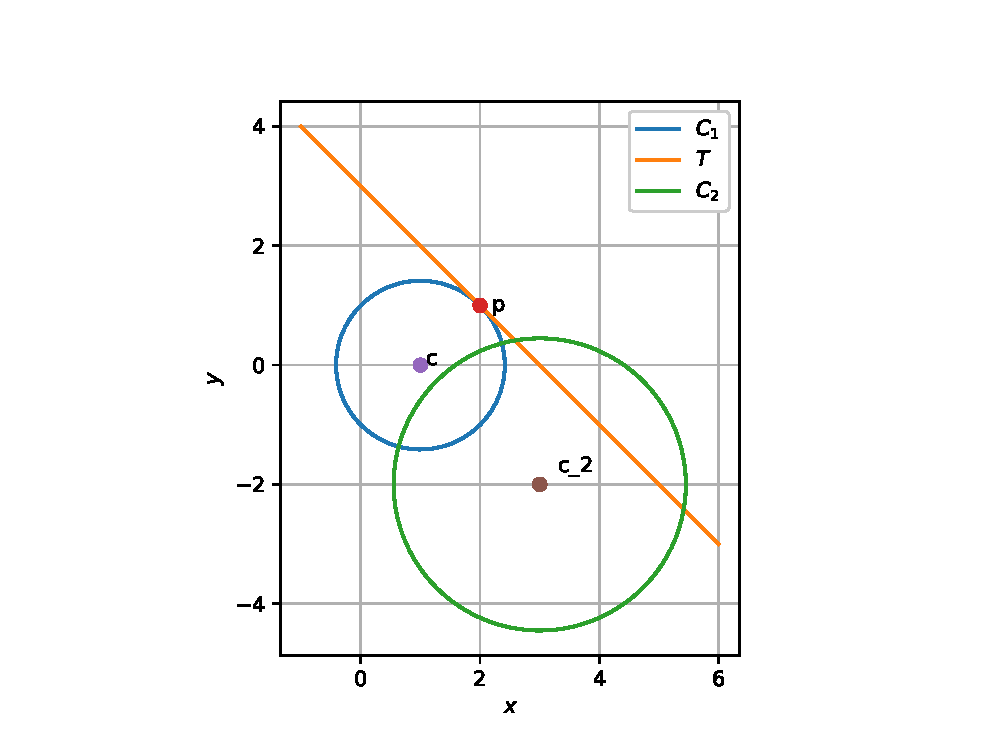
\includegraphics[width=\columnwidth]{./figs/circle.eps}
\caption{}
\label{fig:circle}
\end{figure}

\end{enumerate}
.
 
\subsection{Parabola}
\renewcommand{\theequation}{\theenumi}
\begin{enumerate}[label=\arabic*.,ref=\thesubsection.\theenumi]
\numberwithin{equation}{enumi}
%
\item A standard {\em parabola} has the equation  
\begin{align}
\label{eq:parab_standard}
\vec{x}^T\myvec{0 & 0\\0 & 1}\vec{x}-4a\myvec{1 & 0 }\vec{x}= 0 
\end{align}
\item Any point on \eqref{eq:parab_standard} can be expressed as
\begin{align}
\label{eq:parab_param}
at\myvec{t \\ 2t }
\end{align}
\item Find the tangent at $\myvec{1 \\ 7}$ to the parabola
\begin{equation}
\vec{x}^T\myvec{1 & 0 \\ 0 & 0}\vec{x} + \myvec{0 & -1}\vec{x} + 
6 = 0
\end{equation}
\\
\solution Substituting
\begin{equation}
\vec{p} = \myvec{1 \\ 7}, V = \myvec{1 & 0 \\ 0 & 0}, \vec{u} = \frac{1}{2}\myvec{0 \\ -1}
\end{equation}
%
in \eqref{eq:tangent}, the desired equation is
\begin{multline}
\sbrak{\myvec{ 1 & 7}\myvec{1 & 0 \\ 0 & 0}+\frac{1}{2}\myvec{0 & -1}}\vec{x} 
\\
+ \frac{1}{2}\myvec{ 1 & 7}\myvec{0 \\
-1} 
+6 = 0
\end{multline}
resulting in
\begin{equation}
\myvec{ 2 & -1}\vec{x} 
 = -5
\label{eq:tangent_eg}
\end{equation}
\item The line in \eqref{eq:tangent_eg}
touches the circle
\begin{equation}
\vec{x}^T\vec{x} + 4 \myvec{4 & 3}\vec{x} + c = 0
\label{eq:circle_eg}
\end{equation}
Find $c$.
\\
\solution Comparing \eqref{eq:quadratic_vec} and \eqref{eq:circle_eg},
\begin{align}
\begin{split}
V &= I,
\\
\vec{u} &= 2 \myvec{4 \\ 3}
\end{split}
\end{align}
%
Comparing \eqref{eq:tangent} and \eqref{eq:tangent_eg},
\begin{align}
\vec{p}+2 \myvec{4 \\ 3} &= \myvec{2 \\ -1}
\\
\implies \vec{p} &= -\myvec{6 \\ 7}
%\label{eq:tangent}
\end{align}
%
and
\begin{align}
c +\vec{p}^T\vec{u}&= 5
\\
\implies c &= 5+2\myvec{6 & 7}  \myvec{4 \\ 3}
\\
 &= 95
%\label{eq:tangent}
\end{align}
%
\item 
%Summarize all the above computations through a Python script and 
Plot 
the parabola, tangent and circle.
\\
\solution 
%The following code generates 
See Fig. \ref{fig:parab}.
%\begin{lstlisting}
%wget 
%https://github.com/gadepall/school/raw/master/linalg/2D/manual/codes/parab.py
%\end{lstlisting}
\begin{figure}[!ht]
\centering
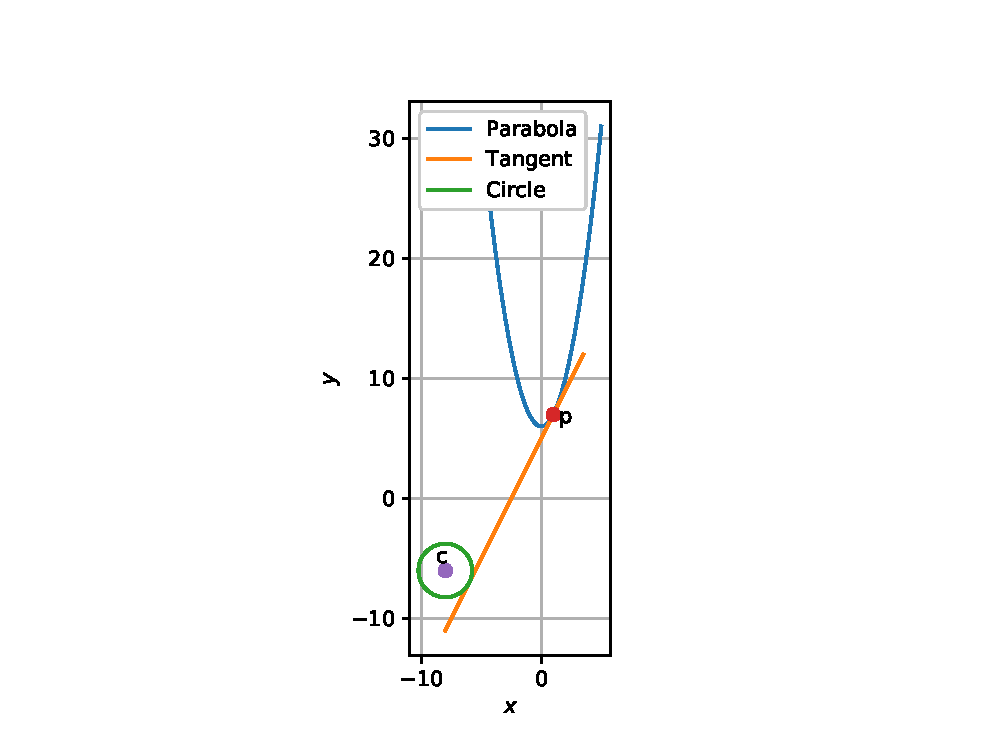
\includegraphics[width=\columnwidth]{./figs/parab.eps}
\caption{}
\label{fig:parab}
\end{figure}
\end{enumerate}
 
\subsection{Affine Transformation}
\renewcommand{\theequation}{\theenumi}
\begin{enumerate}[label=\arabic*.,ref=\thesubsection.\theenumi]
\numberwithin{equation}{enumi}
\item In general, Fig. \ref{fig:parab} was generated using an {\em affine transformation}.

\item Express 
\begin{align}
y_2 = y_1^2
\label{eq:parab}
\end{align}
as a matrix equation.
\\
\solution  \eqref{eq:parab} can be expressed as
\begin{align}
\vec{y}^T\vec{D}\vec{y}+2\vec{g}^T\vec{y} = 0
\label{eq:parab_mat}
\end{align}
%
where 
\begin{align}
\vec{D} = \myvec{1 & 0 \\ 0 & 0} 
,
\vec{g} &= -\frac{1}{2}\myvec{0 \\ 1}
\label{eq:parab_coeffs}
\end{align}
%
\item Given 
\begin{align}
\vec{x}^T\vec{V}\vec{x}+2\vec{u}^T\vec{x}+ F = 0,
\label{eq:parab_gen}
\end{align}
where 
\begin{align}
\vec{V}=\vec{V}^T, \det(\vec{V}) = 0,
\label{eq:parab_vcond}
\end{align}
%
and $\vec{P}, \vec{c}$ such that
\begin{align}
\vec{x} = \vec{P}\vec{y}+\vec{c}.
\label{eq:parab_affine}
\end{align}
\eqref{eq:parab_affine} is known as an affine transformation.
Show that
\begin{align}
\begin{split}
\vec{D} &= \vec{P}^T\vec{V}\vec{P}
\\
\vec{g} &= \vec{P}^T\brak{\vec{V}\vec{c}+\vec{u}}
\\
F+ \vec{c}^T\vec{V}\vec{c} + 2\vec{u}^T\vec{c}&= 0
\end{split}
\label{eq:parab_parmas}
\end{align}

\solution Substituting \eqref{eq:parab_affine} in \eqref{eq:parab_gen},
\begin{align}
\brak{\vec{P}\vec{y}+\vec{c}}^T\vec{V}\brak{\vec{P}\vec{y}+\vec{c}}+2\vec{u}^T\brak{\vec{P}\vec{y}+\vec{c}}+ F = 0, 
\end{align}
which can be expressed as
\begin{multline}
\implies \vec{y}^T\vec{P}^T\vec{V}\vec{P}\vec{y}+2\brak{\vec{V}\vec{c}+\vec{u}}^T\vec{P}\vec{y}
\\
+ F+ \vec{c}^T\vec{V}\vec{c} + 2\vec{u}^T\vec{c} = 0
\label{eq:parab_simp}
\end{multline}
%
Comparing \eqref{eq:parab_simp} with \eqref{eq:parab_mat} \eqref{eq:parab_parmas} is obtained.
%
\item Show that there exists a $\vec{P}$ such that 
\begin{align}
\vec{P}^T\vec{P} = \vec{I}
\end{align}
%
Find $\vec{P}$ using
\begin{align}
\vec{D} = \vec{P}^T\vec{V}\vec{P}
\end{align}
\item Find $\vec{c}$ from \eqref{eq:parab_parmas}.
\\
\solution 
\begin{align}
\because \vec{g} &= \vec{P}^T\brak{\vec{V}\vec{c}+\vec{u}},
\\
\vec{V}\vec{c}&= \vec{P}\vec{g} - \vec{u}
\\
\implies \vec{c}^T\vec{V}\vec{c} &= \vec{c}^T\brak{\vec{P}\vec{g} - \vec{u}} = -F- 2\vec{u}^T\vec{c}
\end{align}
%
resulting in the matrix equation
\begin{align}
\myvec{\vec{V}\\ \brak{\vec{P}\vec{g} + \vec{u}}^T}\vec{c}&= \myvec{\vec{P}\vec{g} - \vec{u}\\ -F}
\end{align}
%
for computing $\vec{c}$.
\end{enumerate}
.
 
\subsection{Ellipse}
\renewcommand{\theequation}{\theenumi}
\begin{enumerate}[label=\arabic*.,ref=\thesubsection.\theenumi]
\numberwithin{equation}{enumi}

\item Express the following equation in the form given in \eqref{eq:quadratic_vec}
\begin{equation}
E:\, 5x_1^2-6x_1x_2 + 5x_2^2+22x_1-26x_2+29=0
\label{eq:ellipse}
\end{equation}
\\
\solution \eqref{eq:ellipse} can be expressed as
\begin{equation}
\vec{x}^TV\vec{x} + 2\vec{u}^T\vec{x}  + 29=0
\label{eq:ellipse_quadc}
\end{equation}
%
where
\begin{equation}
V = \myvec{5 & -3 \\ -3 & 5}, \vec{u} = \myvec{11 \\ -13}
\label{eq:ellipsevu}
\end{equation}
%\item Find $\vec{c}$ and $K$ such that 
%\begin{equation}
%\brak{\vec{x}-\vec{c}}^TV\brak{\vec{x}-\vec{c}} = K 
%\label{eq:ellipsec}
%\end{equation}
%%
%\solution \eqref{eq:ellipsec} can be expressed as
%\begin{align}
%\vec{x}^TV\vec{x}-2\vec{c}^TV\vec{x} +\vec{c}^TV\vec{c}-K = 0.
%\end{align}
%%
%Comparing with \eqref{eq:ellipse_quadc},
%\begin{align}
%V\vec{c}&=-\vec{u}
%\\
%\vec{c}^TV\vec{c} - K &=29
%\\
%\implies \vec{c} &=-V^{-1}\vec{u} = \myvec{-1 \\ 2},
%\\
%\text{and }K& = 8
%\end{align}
%
\item Using the affine transformation in \eqref{eq:affine}, show that 
\eqref{eq:ellipse_quadc} can be expressed as
\begin{equation}
\vec{y}^TD\vec{y}= 1
\label{eq:ellipseo}
\end{equation}
%
where
\begin{align}
\label{eq:ellipse_parmas_d}
\vec{D} &= 
\vec{P}^T\vec{V}\vec{P}
\\
\vec{c}&= -\vec{V}^{-1}\vec{u}
\label{eq:ellipse_parmas_c}
\end{align}
for 
\begin{equation}
\vec{P}^\vec{T}\vec{P} = \vec{I}
\label{eq:ellipse_trans}
\end{equation}
\item Find $\vec{c}$
%For 
\\
\solution 
\begin{align}
%\vec{y}= \frac{P^T\brak{\vec{x}-\vec{c}}}{\sqrt{K}},
\vec{c} = \myvec{1 \\ -2}
%\label{eq:ellipse_xy}
\end{align}
%\eqref{eq:ellipsec} transforms to \eqref{eq:ellipseo}.
\item If 
\begin{align}
D &= \myvec{\lambda_1 & 0 \\ 0 & \lambda_2 }
\\
P &= \myvec{\vec{P}_1 & \vec{P}_2 }
\label{eq:ellipse_eigmat}
\end{align}
show that 
\begin{equation}
V\vec{z} = \lambda \vec{z}
\label{eq:ellipse_eig}
\end{equation}
%
where $\lambda \in \cbrak{\lambda_1, \lambda_2}, \vec{z}\in\cbrak{ \vec{P}_1, \vec{P}_2}$.
\item Find $\lambda$.
\\
\solution $\lambda$ is obtained by solving the following equation.
%\item Find the length of the semi-major and semi-minor axes of $E$.
%\\
%\solution The values are given by
%\begin{align}
%\sqrt{\frac{K}{\lambda}}
%\label{eq:ellipsekl}
%\end{align}
%obtained by solving for $\lambda$ in \eqref{eq:ellipse_eig}.  Thus,
\begin{align}
\abs{\lambda I-V} &= 0
\label{eq:ellipse_ceq}
\\
\implies\begin{vmatrix}\lambda -5 & 3 \\ 3 & \lambda -5\end{vmatrix} & = 0
\\
\implies \lambda^2 -10 \lambda+ 16 &= 0
\\
\implies \lambda &= 2, 8
\end{align}
%Thus, the length of the semi-major axis is 2 and that of the semi-minor axis is 1.
\item Sketch \ref{eq:ellipseo}.
\item Find $\vec{P}_1$ and $\vec{P}_2$.
\\
\solution From \eqref{eq:ellipse_eig}
\begin{align}
V\vec{P}_1 &= \lambda_1 \vec{P}_1
\\
\implies \brak{V-\lambda I} \vec{y}&= 0
\\
\implies \myvec{1 & -1} \vec{P}_1&= 0
\\
\text{or, } \vec{P}_1 = k_1 \myvec{1 \\ 1}
\label{eq:ellipsen1}
\end{align}
%
Similarly, 
%where
%\begin{align}
%\vec{n}_1= \myvec{1 \\ -1}
%\end{align}
%
%Similarly, $\vec{P}_2$ is a point on
\begin{align}
\myvec{1 &  1}\vec{P}_2&= 0
\\
\text{or, } \vec{P}_2 = k_2 \myvec{1 \\ -1}
\end{align}
%
%\begin{align}
%\vec{n}_2= 
%\end{align}
\item Find $\vec{P}$.
\\
\solution From \eqref{eq:ellipse_trans} and \eqref{eq:ellipse_eigmat},
\begin{align}
k_1 &=  \frac{1}{\norm{\myvec{1 \\ 1}}} = \frac{1}{\sqrt{2}}
\\
k_2 &=  \frac{1}{\norm{\myvec{1 \\ -1}}} = \frac{1}{\sqrt{2}}
\end{align}
%
Thus,
\begin{align}
\vec{P} = \frac{1}{\sqrt{2}}\myvec{1 & 1 \\ 1 & -1}
\end{align}

\item Find the equation of the major axis for $E$.
\\
\solution  The major axis for \eqref{eq:ellipseo} is the line
\begin{equation}
\vec{y} = \lambda_1\myvec{1 \\ 0}.
\end{equation}
Using the affine transformation in \eqref{eq:affine}
\begin{align}
\vec{x}= \vec{P}\vec{y}+\vec{c}
\\ 
\implies  \vec{x}-\vec{c}= \lambda_1\vec{P}_1
\\ 
\text{or, }\myvec{1 & -1}\vec{x}&= \myvec{1 & -1}\myvec{1 \\ -2}
\\
&= -3
\end{align}
%
since 
\begin{align}
P\myvec{1 \\ 0}=\vec{P}_1\text{ and } \myvec{1 & -1}\vec{P}_1 = 0
\end{align}
%
which is the major axis of the ellipse $E$.
\item Find the minor axis of $E$.
%
\item Let $\vec{F}_1,\vec{F}_2$ be such that
\begin{equation}
\norm{\vec{x}-\vec{F}_1}
+\norm{\vec{x}-\vec{F}_2} =2k
\end{equation}
Find $\vec{F}_1, \vec{F}_2$ and $k$.
\item 
%Summarize all the above computations through a Python script and 
Plot 
the ellipses in \eqref{eq:ellipse} and \eqref{eq:ellipseo}.
\\
\solution 
%The following script plots 
See Fig. \ref{fig:ellipse} 
%using the 
%principles of an affine transformation. 
%\begin{lstlisting}
%https://github.com/gadepall/school/raw/master/linalg/2D/manual/codes/ellipse.py
%\end{lstlisting}
\begin{figure}[!ht]
\centering
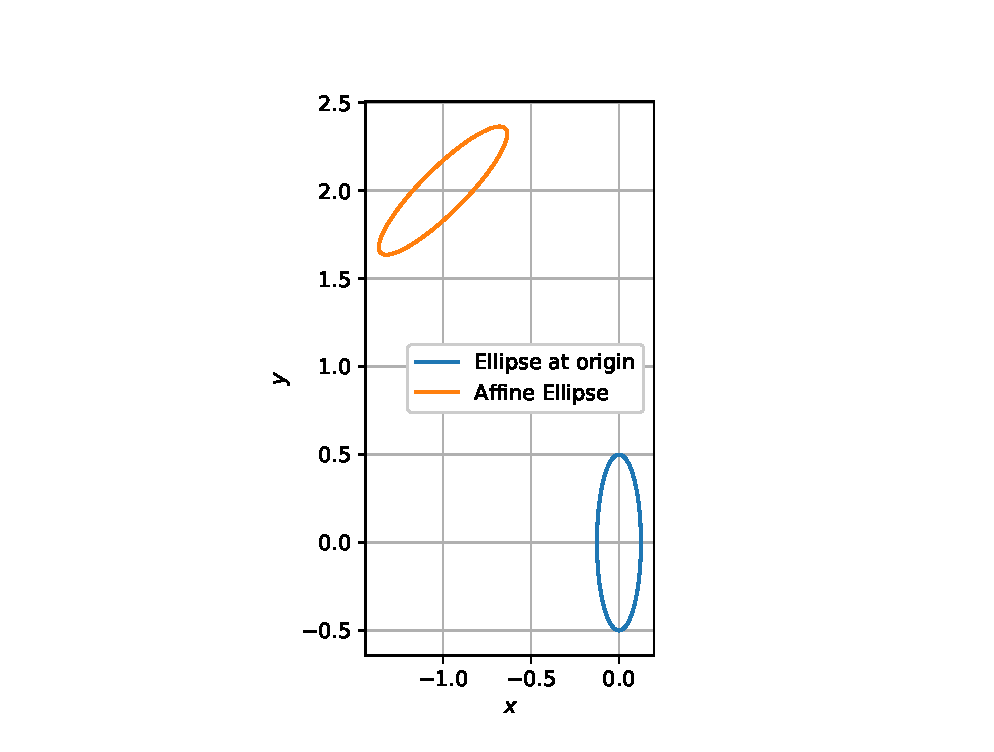
\includegraphics[width=\columnwidth]{./figs/ellipse.eps}
\caption{}
\label{fig:ellipse}
\end{figure}
\end{enumerate}
 
\subsection{Hyperbola}
\renewcommand{\theequation}{\theenumi}
\begin{enumerate}[label=\arabic*.,ref=\thesubsection.\theenumi]
\numberwithin{equation}{enumi}
\item Tangents are drawn to the hyperbola 
\begin{equation}
\vec{x}^TV\vec{x} =36 
\label{eq:hyper}
\end{equation}
%
where
\begin{equation}
V = \myvec{4 & 0 \\ 0 & -1}
\label{eq:hyperv}
\end{equation}
%
at points $\vec{P}$ and $\vec{Q}$.  If these tangents intersect at 
\begin{equation}
\vec{T}= \myvec{0 \\ 3},
\end{equation}
%
find the equation of $PQ$.
\\
\solution The equations of the two tangents are obtained using \eqref{eq:tangent} as
\begin{align}
\vec{P}^TV\vec{x} &=36
\\
\vec{Q}^TV\vec{x}  &=36.
\end{align}		
%
Since both pass through $\vec{T}$
\begin{align}
\label{eq:hyperp}
\vec{P}^TV\vec{T}  &=36 \implies \vec{P}^T\myvec{0  \\  -3} = 36
\\
\vec{Q}^TV\vec{T}  &=36 \implies \vec{Q}^T\myvec{0  \\  -3} = 36
\label{eq:hyperq}
\end{align}
Thus, $\vec{P}, \vec{Q}$ satisfy
\begin{align}
\myvec{0 &  -3}\vec{x} &= -36
\\
\implies \myvec{0 &  1}\vec{x} &= -12
\label{eq:d1}
\end{align}
%
which is the equation of $PQ$.
\item In $\triangle PTQ$, find the equation of the altitude $TD \perp PQ$.
\\
\solution Since 
\begin{align}
 \myvec{1 &  0} \myvec{0 \\  1}=0
\end{align}
using \eqref{eq:line_normal} and \eqref{eq:d1},
the equation of $TD$ is
\begin{align}
\myvec{1 & 0}\brak{\vec{x}-\vec{T}} &= 0
\\
\implies \myvec{1 & 0}\vec{x} &= 0
\label{eq:d2}
\end{align}
%
\item Find $D$.
\\
\solution
From \eqref{eq:d1} and \eqref{eq:d2},
\begin{align}
 \myvec{1 & 0 \\ 0 &  1}\vec{D} &= \myvec{0 \\ -12 }
\\
\implies  \vec{D} &= \myvec{0 \\ -12 }
\label{eq:hyperd}
\end{align}
%
\item Show that the equation of $PQ$ can also be expressed as
\begin{align}
\label{eq:pq_slope}
\vec{x} = \vec{D}+\lambda \vec{m}
\end{align}
where
\begin{align}
\vec{m} &=   \myvec{1 \\ 0}
\label{eq:hyper_slope}
\end{align}
%
\item Show that for $\vec{V}^T = \vec{V}$,
\begin{equation}
\label{eq:quad_md}
\brak{\vec{D}+\lambda\vec{m}}^TV\brak{\vec{D}+\lambda\vec{m}} + F= 0 
\end{equation}
can be expressed as
\begin{equation}
\label{eq:quad_lambda}
\lambda^2\vec{m}^TV\vec{m}+2\lambda\vec{m}^TV\vec{D}+\vec{D}^TV\vec{D}
+ F = 0
\end{equation}
%
\item Find $\vec{P}$ and $\vec{Q}$.
\\
\solution From \eqref{eq:pq_slope} and \eqref{eq:hyper} \eqref{eq:quad_lambda} is obtained.
%
Substituting from \eqref{eq:hyper_slope}, \eqref{eq:hyperv} and \eqref{eq:hyperd}
\begin{align}
\vec{m}^TV\vec{m} &= \myvec{1& 0} \myvec{4 & 0 \\ 0 & -1}\myvec{1 \\ 0} = 4
\\
\vec{m}^TV\vec{D} & = \myvec{1& 0}\myvec{4 & 0 \\ 0 & -1}\myvec{0 \\ -12 } = 0
\\
\vec{D}^TV\vec{D} &= \myvec{0 & -12 }\myvec{4 & 0 \\ 0 & -1}\myvec{0 \\ -12 } = -144
\end{align}
%
Substituting in \eqref{eq:quad_lambda}
\begin{align}
4 \lambda^2 - 144 &= 36
\\
\implies
\lambda &= \pm 3\sqrt{5}
\end{align}
%
Substituting in \eqref{eq:pq_slope},
\begin{align}
\vec{P} &= \vec{D}+ 3\sqrt{5} \vec{m} = 3 \myvec{ \sqrt{5} \\ -4}
\\
\vec{Q} &= \vec{D}- 3\sqrt{5} \vec{m} = -3 \myvec{ \sqrt{5} \\ 4}
\end{align}
%
\item Find the area of $\triangle PTQ$.
\\
\solution Since
\begin{align}
PQ &= \norm{\vec{P}-\vec{Q}} = 6\sqrt{5}
\\
TD &= \norm{\vec{T}-\vec{D}} = 15,
\end{align}
the desired area is
\begin{equation}
\frac{1}{2}PQ \times TD = 45 \sqrt{5}
\end{equation}
\item Repeat the previous exercise using determinants.
\item 
%Summarize all the above computations through a Python script and 
Plot 
the hyperbola.
\\
\solution  See Fig. \ref{fig:hyperbola}
\begin{figure}
\centering
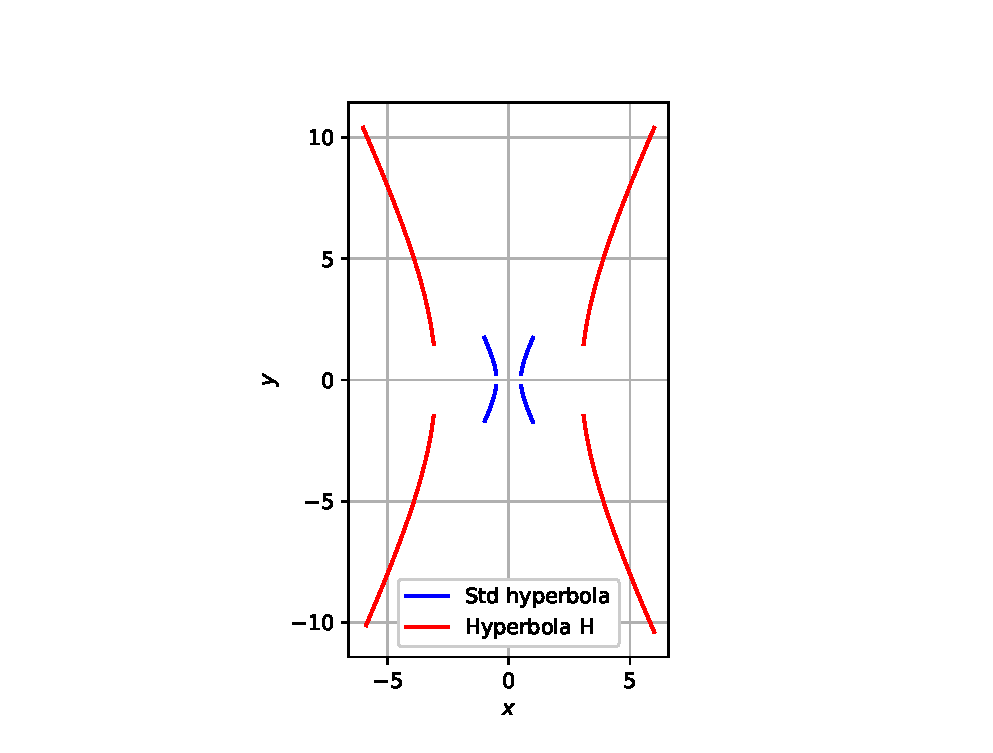
\includegraphics[width=\columnwidth]{./figs/hyperbola.eps}
\caption{}
\label{fig:hyperbola}
\end{figure}

\end{enumerate}

 
\subsection{Tangent}
\renewcommand{\theequation}{\theenumi}
\begin{enumerate}[label=\arabic*.,ref=\thesubsection.\theenumi]
\item Find the equations of the tangents to the following curves at the points specified:
\begin{multicols}{2}
\begin{enumerate}
{\small
\item
$
y=x\brak{x^2-1}, x=2
$
\item
$
y=x^2+\frac{1}{x^2}, x=1
$
\item
$
y=x^3+2x, x=0
$
\item
$
y=\brak{x+\frac{1}{x}}^3, x=2
$
\item
$
y=\brak{x^2-1}^2, x=1
$
\item
$
y=x^3-x+1, x=3
$
\item
$
y=\brak{x-a}^3, x=2a
$
\item
$
y=ax^2+2bx + c, \brak{x_1,y_1}
$
\item
$
y=\frac{x^3}{a^3}+\frac{a^3}{x^3}, x = a
$
\item
$
y = \frac{x^2}{a}+\frac{a^2}{x}, x = a
$
}
\end{enumerate}
\end{multicols}
\numberwithin{equation}{enumi}
\item Find the tangents to the curve 
\begin{align}
\vec{x}^T\myvec{1 & 0\\0 & 0}\vec{x} + \myvec{1 & -1}\vec{x}=0
\end{align}
%
 at the points where it is cut by
the line 
\begin{align}
\myvec{1 & -1}\vec{x} + 4 = 0
\end{align}
and find the point of intersection of the tangents.
\item Prove that the line 
\begin{align}
\myvec{3 & -4}\vec{x}+4=0
\end{align}
touches the curve 
\begin{align}
\vec{x}^T\myvec{1 & -\frac{1}{2}\\ -\frac{1}{2} & 0}\vec{x} + 1 = 0.
\end{align}
\item Find the points on the curve 
\begin{align}
3y=x^3+3x
\end{align}
at which the tangent is
parallel to the line 
\begin{align}
\myvec{5 & -1}\vec{x} = 0
\end{align}
\renewcommand{\theequation}{\theenumi}
\item Find at what points on the curve 
\begin{align}
\vec{x}^T\myvec{1 & 0 \\ 0 & 0}\vec{x}+\myvec{0 & -1}\vec{x}+9 = 0
\end{align}
 the tangents pass through the origin.
\numberwithin{equation}{enumi}
\item Show that there are three points on the curve
\begin{align}
3y=3x^4+8x^3-6x^2
\end{align}
at which the tangents are parallel to the line 
\begin{align}
\myvec{8 & -1}\vec{x} = 0
\end{align}
\item Show that the  line 
\begin{align}
\myvec{0 & 4}\vec{x}=17
\end{align}
meets the curve 
\begin{align}
y = x^2+\frac{1}{x^2}
\end{align}
in four points and that two of the points of intersection of the tangents at these
four points are on the line  
\begin{align}
\myvec{0 & 4}\vec{x}+1=0, 
\end{align}
and two are on the line 
\begin{align}
\myvec{1 & 0}\vec{x}=0.
\end{align}
\end{enumerate}
 
\subsection{More on Tangents}
\renewcommand{\theequation}{\theenumi}
\begin{enumerate}[label=\arabic*.,ref=\thesubsection.\theenumi]
\item Find the equation of the tangents to the following curves at the points stated:
%\begin{multicols}{2}
\begin{enumerate}
\item
$
\vec{x}^T\vec{x} = 25, \myvec{3\\4}
$
\item
$
\vec{x}^T\myvec{4 & 0 \\ 0 & 9}\vec{x} = 2,
 \myvec{\frac{1}{2} \\ \frac{1}{2}}
$
\item
$
\vec{x}^T\myvec{0 & 0 \\ 0 & 1}\vec{x}-4a\myvec{0 & 1}\vec{x}=0, \myvec{a\\2a}
$
\item
$
\vec{x}^T\myvec{b^2 & 0\\0 & a^2}\vec{x}=a^2b^2,
 \myvec{a\cos\theta\\b\sin\theta}
$
\item
$
\vec{x}^T\myvec{1 & 0\\0& -1}\vec{x} = a^2,
 \myvec{a\sec\theta\\b\tan\theta}
$
\item
$
\vec{x}^T\myvec{1 & -\frac{1}{2}\\-\frac{1}{2} & 1}\vec{x}=4,
 \myvec{2\\2}
$
\item
$
\vec{x}^T\vec{x}+\myvec{2 & 4}\vec{x}-20=0, \myvec{3\\1}
$
\item
$
x^3+y^3-3xy^2+a^3 = 0,
 \myvec{a\\a}
$
\end{enumerate}
%\end{multicols}
\item Find the equation of the tangent at the point $\vec{p}$ on each
of the following curves:
%\begin{multicols}{2}
\begin{enumerate}
\item
$
\vec{x}^T\vec{x} = a^2
$
\item
$
\vec{x}^T\myvec{b^2 & 0\\0 & a^2}\vec{x}= a^2b^2
$
\item
$
\vec{x}^T\myvec{0 & 0\\0 & 1}\vec{x}-4a\myvec{1 & 0}\vec{x} = 0
$
\item
$
\vec{x}^T\myvec{0 & \frac{1}{2}\\\frac{1}{2}}\vec{x}-c^2=0
$
\item
$
y^2\brak{x^2-a^2}=a^2\brak{x^2+a^2}
$
\item
$
x^{\frac{2}{3}}+y^{\frac{2}{3}}=a^{\frac{2}{3}}
$
\end{enumerate}
%\end{multicols}
\end{enumerate}
 
\subsection{Normal}
\renewcommand{\theequation}{\theenumi}
\begin{enumerate}[label=\arabic*.,ref=\thesubsection.\theenumi]
\item Find the equations of the normals to the following curves at the given points
\begin{enumerate}
\item
$
\vec{x}^T\vec{x}- \myvec{2 & 4}\vec{x}=3, \myvec{3\\4}
$
\item
$
\vec{x}^T\myvec{1 & 2\\ 2 & 1}\vec{x} = 13, \myvec{1\\2}
$
\item
$
\vec{x}^T\myvec{0 & 0 \\ 0 & 1}\vec{x}-4a\myvec{1 & 0}\vec{x}=0, \myvec{a\\2a}
$
\item
$
\vec{x}^T\myvec{b^2 & 0\\0 & a^2}\vec{x}=a^2b^2, \myvec{a\cos\theta\\b\sin\theta}
$
\item
$
\vec{x}^T\myvec{1 & 0\\0&-4}\vec{x} = 4a^2, \myvec{2a\sec\theta\\a\tan\theta}
$
\item
$
x^3-y^3-3xy^2+a^2 = 0, \myvec{a\\-a}
$
\end{enumerate}
\item Find the equation of the normal at the point $\vec{p}$ on each of the following curves:
\begin{enumerate}
\item
$
\vec{x}^T\vec{x} = a^2
$
\item
$
\vec{x}^T\myvec{b^2 & 0\\0 & a^2}\vec{x}=a^2b^2
$
\item
$
\vec{x}^T\myvec{0 & 0 \\ 0 & 1}\vec{x}-4a\myvec{1 & 0}\vec{x}=0
$
\item
$
\vec{x}^T\myvec{0 & \frac{1}{2}\\ \frac{1}{2} & 0}\vec{x}=c^2
$
\end{enumerate}
\item Prove that for the curve 
\begin{align}
\vec{x}^T\myvec{0 & 0 \\ 0 & 1}\vec{x}-4a\myvec{1 & 0}\vec{x}=0
\end{align}
the subnormal is of constant length.
\item Prove that the portion of any tangent to the curve $x^{\frac{2}{3}}+y^{\frac{2}{3}}=a^{\frac{2}{3}}$ intercepted by the axes is of length $a$.
\item Prove that for the curve $ay^2=x^3$ the subnormal varies as the square of the subtangent.
\item Prove that for the curve $y=ae^{\frac{x}{b}}$ the subtangent is of length $b$.
\item Prove that the area of the triangle formed by the axes and any tangent to the curve 
 \begin{align}
\vec{x}^T\myvec{0 & \frac{1}{2}\\ \frac{1}{2} & 0}\vec{x}=c^2
\end{align}
is $2c^2$.
\item Prove that for the curve $x^my^n=e^{m+n}$ the portion of a tangent intercepted by the axes is divided at the point of contact in the ratio $m:n$.
\item Prove that, if $N$ is the foot of the ordinate and $NT$ is the subtangent at a point on the
curve 
\begin{align}
\vec{x}^T\myvec{b^2 & 0\\0 & a^2}\vec{x}=a^2b^2, \myvec{a\cos\theta\\b\sin\theta}
\end{align}
 then $OT.ON=a^2$.
\item Prove that the perpendicular from the foot of the ordinate to the tangent to a curve is of length
$\frac{y}{\sqrt{\cbrak{1+\brak{\frac{dy}{dx}}^2}}}$.  Show that for the curve $y = c\cosh \frac{x}{c}$, this perpendicular is of length $c$.
\item Find the equation of the tangent to the curve 
\numberwithin{equation}{enumi}
\begin{align}
2x^3+2y^3 - 9axy = 0
\end{align}
at the point $\myvec{2a\\a}$; and show that the tangent meets the curve again where 
\begin{align}
\myvec{4 & 1}\vec{x} = 0
\end{align}
\end{enumerate}
 
\subsection{Affine Transformation: Exercises}
\renewcommand{\theequation}{\theenumi}
\begin{enumerate}[label=\arabic*.,ref=\thesubsection.\theenumi]
\item What does the equation 
\begin{align}
\vec{x}^T\myvec{1 & 0\\0 & -1}\vec{x}-\myvec{4 & 6}\vec{x}-6=0
\end{align}
become when the origin is moved to the point $\myvec{2\\-3}$?
\\
\solution
Let the balanced version of (\ref{eq:solutions/chem/6ato balance}) be
\begin{align}
    \label{eq:solutions/chem/6abalanced}x_{1}HNO_{3}+ x_{2}Ca(OH)_{2}\to x_{3}Ca(NO_{3})_{2}+ x_{4}H_{2}O
\end{align}

which results in the following equations:
\begin{align}
    (x_{1}+ 2x_{2}-2x_{4}) H= 0\\
    (x_{1}-2x_{3}) N= 0\\
    (3x_{1}+ 2x_{2}-6x_{3}- x_{4}) O=0\\
    (x_{2}-x_{3}) Ca= 0
\end{align}

which can be expressed as
\begin{align}
    x_{1}+ 2x_{2}+ 0.x_{3} -2x_{4} = 0\\
    x_{1}+ 0.x_{2} -2x_{3} +0.x_{4}= 0\\
    3x_{1}+ 2x_{2}-6x_{3}- x_{4} =0\\
    0.x_{1} +x_{2}-x_{3} +0.x_{4}= 0
\end{align}

resulting in the matrix equation
\begin{align}
    \label{eq:solutions/chem/6a matrix}
    \myvec{1 & 2 & 0 & -2\\
           1 & 0 & -2 & 0\\
           3 & 2 & -6 & -1\\
           0 & 1 & -1 & 0}\vec{x}
           =\vec{0}
\end{align}

where,
\begin{align}
   \vec{x}= \myvec{x_{1}\\x_{2}\\x_{3}\\x_{4}}
\end{align}

(\ref{eq:solutions/chem/6a matrix}) can be reduced as follows:
\begin{align}
    \myvec{1 & 2 & 0 & -2\\
           1 & 0 & -2 & 0\\
           3 & 2 & -6 & -1\\
           0 & 1 & -1 & 0}
    \xleftrightarrow[R_{3}\leftarrow \frac{R_3}{3}-R_{1}]{R_{2}\leftarrow R_2- R_1}
    \myvec{1 & 2 & 0 & -2\\
           0 & -2 & -2 & 2\\
           0 & -\frac{4}{3} & -2 & \frac{5}{3}\\
           0 & 1 & -1 & 0}\\
    \xleftrightarrow{R_2 \leftarrow -\frac{R_2}{2}}
    \myvec{1 & 2 & 0 & -2\\
          0 & 1 & 1 & -1\\
          0 & -\frac{4}{3} & -2 & \frac{5}{3}\\
          0 & 1 & -1 & 0}\\
    \xleftrightarrow[R_4 \leftarrow R_4- R_2]{R_3 \leftarrow R_3 + \frac{4}{3}R_2}
    \myvec{1 & 2 & 0 & -2\\
           0 & 1 & 1 & -1\\
           0 & 0 & -\frac{2}{3} & \frac{1}{3}\\
           0 & 0 & -2 & 1}\\
    \xleftrightarrow[R_3 \leftarrow -\frac{3}{2}R_3]{R_1 \leftarrow R_1- 2R_2}
    \myvec{1 & 0 & -2 & 0\\
           0 & 1 & 1 & -1\\
           0 & 0 & 1 & -\frac{1}{2}\\
           0 & 0 & -2 & 1}\\
    \xleftrightarrow{R_4\leftarrow R_4 + 2R_3}
    \myvec{1 & 0 & -2 & 0\\
           0 & 1 & 1 & -1\\
           0 & 0 & 1 & -\frac{1}{2}\\
           0 & 0 & 0 & 0}\\
    \xleftrightarrow[R_2\leftarrow R_2-R_3]{R_1\leftarrow R_1 + 2R_3}
    \myvec{1 & 0 & 0 & -1\\
           0 & 1 & 0 & -\frac{1}{2}\\
           0 & 0 & 1 & -\frac{1}{2}\\
           0 & 0 & 0 & 0}
\end{align}

Thus,
\begin{align}
    x_1=x_4, x_2= \frac{1}{2}x_4, x_3=\frac{1}{2}x_4\\
    \implies \quad\vec{x}= x_4\myvec{1\\ \frac{1}{2}\\ \frac{1}{2}\\1} =\myvec{2\\1\\1\\2}
\end{align} 
by substituting $x_4= 2$.

\hfill\break
%\vspace{5mm} 
Hence, (\ref{eq:solutions/chem/6abalanced}) finally becomes
\begin{align}
    2HNO_{3}+ Ca(OH)_{2}\to Ca(NO_{3})_{2}+ 2H_{2}O
\end{align}

\item To what point must the origin be moved in order that the equation
\begin{align}
\vec{x}^T\myvec{2 & -\frac{3}{2}\\ -\frac{3}{2} & 4}\vec{x}+\myvec{10 & -19}\vec{x}+23=0
\end{align}
may become
\begin{align}
\vec{x}^T\myvec{2 & -\frac{3}{2}\\ -\frac{3}{2} & 4}\vec{x} = 1
\end{align}
\item Show that the equation
\begin{align}
\vec{x}^T\vec{x}= a^2
\end{align}
remains unaltered by any rotation of the axes.
\item What does the equation
\begin{align}
\vec{x}^T\myvec{1 & \sqrt{3}\\ \sqrt{3} & -1}\vec{x} = 2a^2
\end{align}
become when the axes are turned through $30\degree$?
\item What does the equation
\begin{align}
\vec{x}^T\myvec{1 & -1\\-1 & 1}\vec{x}-4\sqrt{2}a\myvec{1 & 1}\vec{x}=0
\end{align}
become when the axes are turned through $45\degree$?
\item To what point must the origin be moved in order that the equation
\begin{align}
    \vec{x}^T\myvec{1 & 2\\2 & -2}\vec{x}+\myvec{10 & -4}\vec{x}=0 \label{eq:solutions/3/4/6/eq:q1}
\end{align}
may become
\begin{align}
    \vec{x}^T\myvec{1 & 2\\2 & -2}\vec{x}=1\label{eq:solutions/3/4/6/eq:q2}
\end{align}
and through what angle must the axes be turned in order to obtain
\begin{align}
    \vec{x}^T\myvec{p & 0\\0 & q}\vec{x}=1\label{eq:solutions/3/4/6/eq:q3}
\end{align}
\solution
Let the balanced version of (\ref{eq:solutions/chem/6ato balance}) be
\begin{align}
    \label{eq:solutions/chem/6abalanced}x_{1}HNO_{3}+ x_{2}Ca(OH)_{2}\to x_{3}Ca(NO_{3})_{2}+ x_{4}H_{2}O
\end{align}

which results in the following equations:
\begin{align}
    (x_{1}+ 2x_{2}-2x_{4}) H= 0\\
    (x_{1}-2x_{3}) N= 0\\
    (3x_{1}+ 2x_{2}-6x_{3}- x_{4}) O=0\\
    (x_{2}-x_{3}) Ca= 0
\end{align}

which can be expressed as
\begin{align}
    x_{1}+ 2x_{2}+ 0.x_{3} -2x_{4} = 0\\
    x_{1}+ 0.x_{2} -2x_{3} +0.x_{4}= 0\\
    3x_{1}+ 2x_{2}-6x_{3}- x_{4} =0\\
    0.x_{1} +x_{2}-x_{3} +0.x_{4}= 0
\end{align}

resulting in the matrix equation
\begin{align}
    \label{eq:solutions/chem/6a matrix}
    \myvec{1 & 2 & 0 & -2\\
           1 & 0 & -2 & 0\\
           3 & 2 & -6 & -1\\
           0 & 1 & -1 & 0}\vec{x}
           =\vec{0}
\end{align}

where,
\begin{align}
   \vec{x}= \myvec{x_{1}\\x_{2}\\x_{3}\\x_{4}}
\end{align}

(\ref{eq:solutions/chem/6a matrix}) can be reduced as follows:
\begin{align}
    \myvec{1 & 2 & 0 & -2\\
           1 & 0 & -2 & 0\\
           3 & 2 & -6 & -1\\
           0 & 1 & -1 & 0}
    \xleftrightarrow[R_{3}\leftarrow \frac{R_3}{3}-R_{1}]{R_{2}\leftarrow R_2- R_1}
    \myvec{1 & 2 & 0 & -2\\
           0 & -2 & -2 & 2\\
           0 & -\frac{4}{3} & -2 & \frac{5}{3}\\
           0 & 1 & -1 & 0}\\
    \xleftrightarrow{R_2 \leftarrow -\frac{R_2}{2}}
    \myvec{1 & 2 & 0 & -2\\
          0 & 1 & 1 & -1\\
          0 & -\frac{4}{3} & -2 & \frac{5}{3}\\
          0 & 1 & -1 & 0}\\
    \xleftrightarrow[R_4 \leftarrow R_4- R_2]{R_3 \leftarrow R_3 + \frac{4}{3}R_2}
    \myvec{1 & 2 & 0 & -2\\
           0 & 1 & 1 & -1\\
           0 & 0 & -\frac{2}{3} & \frac{1}{3}\\
           0 & 0 & -2 & 1}\\
    \xleftrightarrow[R_3 \leftarrow -\frac{3}{2}R_3]{R_1 \leftarrow R_1- 2R_2}
    \myvec{1 & 0 & -2 & 0\\
           0 & 1 & 1 & -1\\
           0 & 0 & 1 & -\frac{1}{2}\\
           0 & 0 & -2 & 1}\\
    \xleftrightarrow{R_4\leftarrow R_4 + 2R_3}
    \myvec{1 & 0 & -2 & 0\\
           0 & 1 & 1 & -1\\
           0 & 0 & 1 & -\frac{1}{2}\\
           0 & 0 & 0 & 0}\\
    \xleftrightarrow[R_2\leftarrow R_2-R_3]{R_1\leftarrow R_1 + 2R_3}
    \myvec{1 & 0 & 0 & -1\\
           0 & 1 & 0 & -\frac{1}{2}\\
           0 & 0 & 1 & -\frac{1}{2}\\
           0 & 0 & 0 & 0}
\end{align}

Thus,
\begin{align}
    x_1=x_4, x_2= \frac{1}{2}x_4, x_3=\frac{1}{2}x_4\\
    \implies \quad\vec{x}= x_4\myvec{1\\ \frac{1}{2}\\ \frac{1}{2}\\1} =\myvec{2\\1\\1\\2}
\end{align} 
by substituting $x_4= 2$.

\hfill\break
%\vspace{5mm} 
Hence, (\ref{eq:solutions/chem/6abalanced}) finally becomes
\begin{align}
    2HNO_{3}+ Ca(OH)_{2}\to Ca(NO_{3})_{2}+ 2H_{2}O
\end{align}

\item Through what angle must the axes be turned to reduce the equation
\begin{align}
\vec{x}^T\myvec{1 & -1\\-1 & -1}\vec{x}=1
\end{align}
to the form
\begin{align}
\vec{x}^T\myvec{0 & \frac{1}{2}\\ \frac{1}{2} & 0}\vec{x} = c
\end{align}
where $c$ is a constant.
\item Show that, by changing the origin, the equation
\begin{align}
2\vec{x}^T\vec{x}+\myvec{7 & 5}\vec{x} - 13 = 0
\end{align}
can be transformed to 
\begin{align}
8\vec{x}^T\vec{x} = 89
\end{align}
\item Show that, by rotating the axes, the equation
\begin{align}
\vec{x}^T\myvec{3 & \frac{7}{2}\\ \frac{7}{2} & -3}\vec{x}= 1
\end{align}
can be reduced to 
\begin{align}
\sqrt{85}\vec{x}^T\myvec{1 & 0\\ 0 & -1}\vec{x}= 2
\end{align}
\item Show that, by rotating the axes, the equation
\begin{align}
\vec{x}^T\myvec{41 & 12\\ 12 & 34}\vec{x}= 75
\label{eq:solutions/3/4/9/1}
\end{align}
can be reduced to 
\begin{align}
\vec{x}^T\myvec{2 & 0\\ 0 & 1}\vec{x}= 3
\end{align}
\\
\solution
Let the balanced version of (\ref{eq:solutions/chem/6ato balance}) be
\begin{align}
    \label{eq:solutions/chem/6abalanced}x_{1}HNO_{3}+ x_{2}Ca(OH)_{2}\to x_{3}Ca(NO_{3})_{2}+ x_{4}H_{2}O
\end{align}

which results in the following equations:
\begin{align}
    (x_{1}+ 2x_{2}-2x_{4}) H= 0\\
    (x_{1}-2x_{3}) N= 0\\
    (3x_{1}+ 2x_{2}-6x_{3}- x_{4}) O=0\\
    (x_{2}-x_{3}) Ca= 0
\end{align}

which can be expressed as
\begin{align}
    x_{1}+ 2x_{2}+ 0.x_{3} -2x_{4} = 0\\
    x_{1}+ 0.x_{2} -2x_{3} +0.x_{4}= 0\\
    3x_{1}+ 2x_{2}-6x_{3}- x_{4} =0\\
    0.x_{1} +x_{2}-x_{3} +0.x_{4}= 0
\end{align}

resulting in the matrix equation
\begin{align}
    \label{eq:solutions/chem/6a matrix}
    \myvec{1 & 2 & 0 & -2\\
           1 & 0 & -2 & 0\\
           3 & 2 & -6 & -1\\
           0 & 1 & -1 & 0}\vec{x}
           =\vec{0}
\end{align}

where,
\begin{align}
   \vec{x}= \myvec{x_{1}\\x_{2}\\x_{3}\\x_{4}}
\end{align}

(\ref{eq:solutions/chem/6a matrix}) can be reduced as follows:
\begin{align}
    \myvec{1 & 2 & 0 & -2\\
           1 & 0 & -2 & 0\\
           3 & 2 & -6 & -1\\
           0 & 1 & -1 & 0}
    \xleftrightarrow[R_{3}\leftarrow \frac{R_3}{3}-R_{1}]{R_{2}\leftarrow R_2- R_1}
    \myvec{1 & 2 & 0 & -2\\
           0 & -2 & -2 & 2\\
           0 & -\frac{4}{3} & -2 & \frac{5}{3}\\
           0 & 1 & -1 & 0}\\
    \xleftrightarrow{R_2 \leftarrow -\frac{R_2}{2}}
    \myvec{1 & 2 & 0 & -2\\
          0 & 1 & 1 & -1\\
          0 & -\frac{4}{3} & -2 & \frac{5}{3}\\
          0 & 1 & -1 & 0}\\
    \xleftrightarrow[R_4 \leftarrow R_4- R_2]{R_3 \leftarrow R_3 + \frac{4}{3}R_2}
    \myvec{1 & 2 & 0 & -2\\
           0 & 1 & 1 & -1\\
           0 & 0 & -\frac{2}{3} & \frac{1}{3}\\
           0 & 0 & -2 & 1}\\
    \xleftrightarrow[R_3 \leftarrow -\frac{3}{2}R_3]{R_1 \leftarrow R_1- 2R_2}
    \myvec{1 & 0 & -2 & 0\\
           0 & 1 & 1 & -1\\
           0 & 0 & 1 & -\frac{1}{2}\\
           0 & 0 & -2 & 1}\\
    \xleftrightarrow{R_4\leftarrow R_4 + 2R_3}
    \myvec{1 & 0 & -2 & 0\\
           0 & 1 & 1 & -1\\
           0 & 0 & 1 & -\frac{1}{2}\\
           0 & 0 & 0 & 0}\\
    \xleftrightarrow[R_2\leftarrow R_2-R_3]{R_1\leftarrow R_1 + 2R_3}
    \myvec{1 & 0 & 0 & -1\\
           0 & 1 & 0 & -\frac{1}{2}\\
           0 & 0 & 1 & -\frac{1}{2}\\
           0 & 0 & 0 & 0}
\end{align}

Thus,
\begin{align}
    x_1=x_4, x_2= \frac{1}{2}x_4, x_3=\frac{1}{2}x_4\\
    \implies \quad\vec{x}= x_4\myvec{1\\ \frac{1}{2}\\ \frac{1}{2}\\1} =\myvec{2\\1\\1\\2}
\end{align} 
by substituting $x_4= 2$.

\hfill\break
%\vspace{5mm} 
Hence, (\ref{eq:solutions/chem/6abalanced}) finally becomes
\begin{align}
    2HNO_{3}+ Ca(OH)_{2}\to Ca(NO_{3})_{2}+ 2H_{2}O
\end{align}

\item Show that, by a change of origin and the directions of the coordinate axes, the equation
\begin{align}
\vec{x}^T\myvec{5 & 1\\ 1 & 5}\vec{x}-\myvec{14 & 22}\vec{x}+27= 0
\end{align}
can be transformed to
\begin{align}
\vec{x}^T\myvec{3 & 0\\ 0 & 2}\vec{x}= 1
\end{align}
or
\begin{align}
\vec{x}^T\myvec{2 & 0\\ 0 & 3}\vec{x}= 1
\end{align}
\end{enumerate}
 
%\newpage
\section{Circle}
\subsection{Properties}
\renewcommand{\theequation}{\theenumi}
\begin{enumerate}[label=\arabic*.,ref=\thesubsection.\theenumi]
\item The equation of a circle is 
\begin{align}
\label{eq:circ_norm}
\norm{\vec{x}-\vec{c}} = r
\end{align}
%
where $\vec{c}$ is the centre and $r$ is the radius.
\item By expanding \eqref{eq:circ_norm}, the equation of a circle can also be expressed as
%
\numberwithin{equation}{enumi}
\begin{align}
\norm{\vec{x}-\vec{c}}^2 = r^2&
\\
\implies \vec{x}^T\vec{x}-2\vec{c}^T\vec{x} + \vec{c}^T\vec{c}-r^2 = 0
\label{eq:circ_quad}
\end{align}
\item The direction vector of {\em normal to the circle}  in \eqref{eq:circ_quad} at point $\vec{p}$ is
\begin{align}
\label{eq:circ_normal}
\vec{n} = k\brak{\vec{p}-\vec{c}},
\end{align}
%
where $k$ is a constant.
\item Find the equation of a circle that passes through the points $\vec{A},\vec{B},\vec{C}$.
\\
\solution From \eqref{eq:circ_quad},
\begin{align}
%\label{eq:circ_quad}
\norm{\vec{A}-\vec{c}}^2 = \norm{\vec{B}-\vec{c}}^2 = \norm{\vec{C}-\vec{c}}^2 &= r^2
\\
\implies \norm{\vec{A}-\vec{c}}^2 - \norm{\vec{B}-\vec{c}}^2 &=0
\end{align}
which can be simplified to obtain
\begin{align}
\brak{\vec{A}-\vec{B}}^T\vec{c}=\frac{\norm{\vec{A}}^2 - \norm{\vec{B}}^2}{2}& \quad \text{and}
\\
\brak{\vec{A}-\vec{C}}^T\vec{c}=\frac{\norm{\vec{A}}^2 - \norm{\vec{C}}^2}{2}& 
\end{align}
%
Solving the two yields $\vec{c}$, which can then be used to obtain $r$.
\item Let $\vec{A},\vec{B}$ and $\vec{C}$ be three points on the circle and 
$D$ be a point on $BC$ such that
$OD \perp BC$ as in Fig. \ref{fig:ccircle}.  Show that 
\begin{align}
\vec{D}=\frac{\vec{B}+\vec{C}}{2}
\end{align}
%
\begin{figure}[!ht]
	\begin{center}
		
		%\includegraphics[width=\columnwidth]{./figs/ch3_angle_bisector}
		%\vspace*{-10cm}
		\resizebox{\columnwidth}{!}{\begin{tikzpicture}
[scale=2,>=stealth,point/.style={draw,circle,fill = black,inner sep=0.5pt},]

%\node (D) at (0, 0)[point,label=below :$D$] {};
\node (B) at (-2, -2)[point,label=below left :$B$]{};
\node (A) at (1, 3)[point,label=above:$A$]{};
\node (C) at (4, -1)[point,label=below right:$C$]{};
%\coordinate [point, label={above : $O$ }] (I) at  (1.147, 1.143);
\node (O) at (0.7962963,-0.27777778)[point,label=above:$O$]{};
\node (D) at ( 1,-1.5)[point,label=below:$D$]{};
%\node (x1) at (0.601,-1.357)[point,label=left:$x_1$]{};
%\node (x2) at (2.15,-1.1)[point,label=right:$x_2$]{};
%\node (temp) at ($(O)!0.5!(D)$)[label=right:$r$]{};
%\node (D) at (2.424,1.1)[point,label=above right:$D$]{};
%\node (E) at (1.1, 1.9)[point,label=above right:$E$]{};
%\node (F) at (-1.1, 1.9)[point,label=above left:$F$]{};
\def\rad{3.284101453883}
\draw (O) circle (\rad);

\draw (D)--(O);
\draw (A)--(B);
\draw (B)--(C);
\draw (A)--(C);
%\draw (C)--(D);
%\draw [thick,dashed] (x1) -- (x2);
%\draw [thick,dashed] (O) -- (E);
%\draw [thick,dashed] (O) -- (F);
%\draw (B)--(O);
%\draw (C)--(O);

%\tkzMarkRightAngle[size=.2](A,D,C)
%\tkzMarkRightAngle[size=.15](B,F,O);
%\tkzMarkRightAngle[size=.15](C,E,O);
%\tkzMarkAngle[size=.4](D,B,O);
%\tkzMarkAngle[size=.35](O,B,F);
%\tkzMarkAngle[size=.54](E,C,O);
%\tkzMarkAngle[size=.5](E,C,O);
%\tkzMarkAngle[size=.6](O,C,D);
%\tkzMarkAngle[size=.65](O,C,D);

\end{tikzpicture}}
	\end{center}
	\caption{Circumcircle.}
	\label{fig:ccircle}	
\end{figure}


\solution From \eqref{eq:circ_norm}
\begin{align}
\norm{\vec{B}-\vec{O}}^2=\norm{\vec{C}-\vec{O}}^2=r^2
\\
 \implies \brak{\vec{B}-\vec{O}}^T\brak{\vec{B}-\vec{O}} = 
\brak{\vec{C}-\vec{O}}^T\brak{\vec{C}-\vec{O}} 
\\
 \implies \brak{\vec{B}-\vec{C}}^T\brak{\frac{\vec{B}+\vec{C}}{2} - 
\vec{O}}  = 0
\label{eq:circle_mid}
\end{align}
after simplification. Since $OD \perp BC$,
\begin{align}
\brak{\vec{B}-\vec{C}}^T\brak{\vec{D}-\vec{O}} = 0 
\label{eq:circle_D}
\end{align}
Since $D$ and $\frac{\vec{B}+\vec{C}}{2}$ lie on $BC$, using 
\eqref{eq:line_ab},
\begin{align}
\label{eq:circle_mid_D1}
\frac{\vec{B}+\vec{C}}{2}
&= \vec{B}+ \lambda_1\brak{\vec{B}-\vec{C}}
\\
\vec{D}
&= \vec{B}+ \lambda_2\brak{\vec{B}-\vec{C}}
\label{eq:circle_mid_D2}
\end{align}
Multiplying \eqref{eq:circle_mid_D1} and \eqref{eq:circle_mid_D2} with 
$\brak{\vec{B}-\vec{C}}^T$ and subtracting, $\lambda_1=\lambda_2$
%
\begin{align}
\implies \vec{D} = \frac{\vec{B}+\vec{C}}{2}
\label{eq:circle_bisect}
\end{align}
%
\item Let  $\vec{D}$ be the mid point of $BC$.  Show that $OD \perp BC$.
%
\item The circle with centre $\vec{O}$ and radius $r$ in Fig.\ref{fig:ang_bisect}	
 is inside 
$\triangle ABC$ and touches $AB, BC$ 
and $CA$ at $\vec{F}, \vec{D}$ and $\vec{E}$ respectively. $AB, BC$ and 
$CA$ are known as {\em tangents} to the circle.
\begin{figure}[!ht]
	\begin{center}
		
		%\includegraphics[width=\columnwidth]{./figs/ch3_angle_bisector}
		%\vspace*{-10cm}
		\resizebox{\columnwidth}{!}{\begin{tikzpicture}
[scale=2,>=stealth,point/.style={draw,circle,fill = black,inner sep=0.5pt},]

%\node (D) at (0, 0)[point,label=below :$D$] {};
\node (B) at (-2, -2)[point,label=below left :$B$]{};
\node (A) at (1, 3)[point,label=above:$A$]{};
\node (C) at (4, -1)[point,label=below right:$C$]{};
%\coordinate [point, label={above : $O$ }] (I) at  (1.147, 1.143);
\node (O) at (1.147, 0.143)[point,label=above:$O$]{};
\node (D) at (1.41,-1.43)[point,label=below:$D$]{};
\node (x1) at (0.601,-1.357)[point,label=left:$x_1$]{};
\node (x2) at (2.15,-1.1)[point,label=right:$x_2$]{};
\node (temp) at ($(O)!0.5!(D)$)[label=right:$r$]{};
%\node (D) at (2.424,1.1)[point,label=above right:$D$]{};
%\node (E) at (1.1, 1.9)[point,label=above right:$E$]{};
%\node (F) at (-1.1, 1.9)[point,label=above left:$F$]{};
\def\rad{1.596}
\draw (O) circle (\rad);

\draw (D)--(O);
\draw (A)--(B);
\draw (B)--(C);
\draw (A)--(C);
%\draw (C)--(D);
\draw [thick,dashed] (x1) -- (x2);
%\draw [thick,dashed] (O) -- (E);
%\draw [thick,dashed] (O) -- (F);
%\draw (B)--(O);
%\draw (C)--(O);

%\tkzMarkRightAngle[size=.2](A,D,C)
%\tkzMarkRightAngle[size=.15](B,F,O);
%\tkzMarkRightAngle[size=.15](C,E,O);
%\tkzMarkAngle[size=.4](D,B,O);
%\tkzMarkAngle[size=.35](O,B,F);
%\tkzMarkAngle[size=.54](E,C,O);
%\tkzMarkAngle[size=.5](E,C,O);
%\tkzMarkAngle[size=.6](O,C,D);
%\tkzMarkAngle[size=.65](O,C,D);

\end{tikzpicture}}
	\end{center}
	\caption{Tangent and incircle.}
	\label{fig:ang_bisect}	
\end{figure}


\item Show that $OD \perp BC$.
%\begin{figure}[!h]
%\centering
%\resizebox {\columnwidth} {!} {
%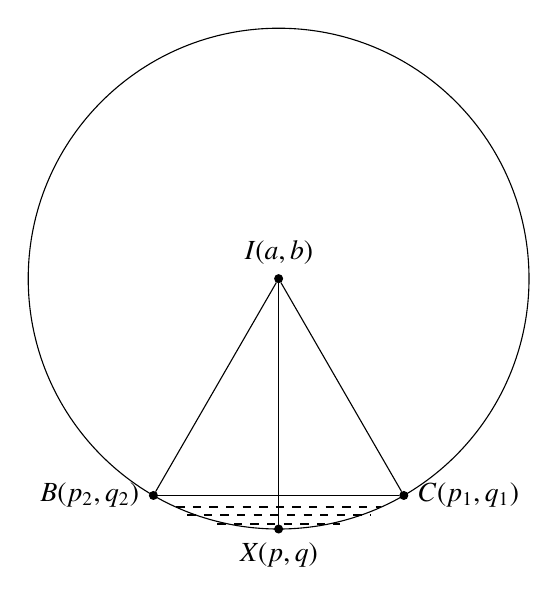
\begin{tikzpicture}
[
scale =2,
>=stealth,
point/.style = {draw, circle, fill = black, inner sep = 1pt},
]

\def\rad{1.59}
\coordinate [point, label={above : $I{(a,b)}$ }] (I) at (0, 0);
\draw (I) circle (\rad);

\node (C) at (300:{\rad})[point,label = right:$C{(p_1,q_1)}$] {};

\node (X) at (270:{\rad}) [point,label = below:$X{(p,q)}$] {};

\node (B) at (240:{\rad}) [point,label = left:$B{(p_2,q_2)}$] {};

\draw (C) -- (I);
\draw (B) -- (I);
\draw (B) -- (C);
\draw (I) -- (X);

\draw[black,thick,dashed](-0.65,-1.45) -- (0.65,-1.45);
\draw[black,thick,dashed](-0.58,-1.5) -- (0.58,-1.5);
\draw[black,thick,dashed](-0.39,-1.56) -- (0.39,-1.56);
\end{tikzpicture}

%}
%\caption{Notion of the derivative.}
%\label{fig:derivative}
%\end{figure}
\\
\solution Let $\vec{x}_1,\vec{x}_2$ be two points on the circle such that 
$x_1x_2 \parallel BC$. Then
%
\begin{align}
\norm{\vec{x}_1-\vec{O}}^2- 
\norm{\vec{x}_2-\vec{O}}^2 &= 0 
\\
\implies 
\brak{\vec{x}_1-\vec{x}_2}^T\brak{\frac{\vec{x}_1+\vec{x}_2}{2}-\vec{O}} &= 
0 
\\
\implies 
\brak{\vec{B}-\vec{C}}^T\brak{\frac{\vec{x}_1+\vec{x}_2}{2}-\vec{O}} &= 
0 
%\label{eq:circle_bisect}
\end{align}
%
For $\vec{x}_1=\vec{x}_2=\vec{D}$, $x_1x_2$ merges into $BC$ and the above 
equation becomes 
%
\begin{align}
\brak{\vec{B}-\vec{C}}^T\brak{\vec{D}-\vec{O}} = 
0 
\implies OD \perp BC
%\label{eq:circle_bisect}
\end{align}
%
\item Give an alternative proof for the above.
\\
\solution Let 
\begin{align}
\vec{B} & = \mbf{0}
\\
\vec{D} &= \lambda \vec{m}
\end{align}
Then
\begin{align}
\norm{\vec{D} - \vec{O}}^2 = r^2 &
\\
\implies \lambda^2\norm{\vec{m}}^2 - 2\lambda\vec{m}^T\vec{O} + \norm{\vec{O}}^2 &= r^2 
\end{align}
Since the above equation has a single root,
\begin{align}
\lambda = \frac{\vec{m}^T\vec{O}}{\norm{\vec{m}}^2}
\label{eq:incircle_lam}
\end{align}
%
Thus, 
\begin{align}
\brak{\vec{D} - \vec{B}}^T\brak{\vec{D} - \vec{O}}
&= \brak{\lambda\vec{m}}^T
\brak{\lambda\vec{m}-\vec{O}}
\\
&=\lambda^2\norm{\vec{m}}^2-\lambda\vec{m}^T\vec{O}
\\
&= \mbf{O} \text{ (from \ref{eq:incircle_lam})}.
\\
\implies & OD \perp BC
\end{align}
\item Find the equation of the tangent at $\vec{D}$.
\\
\solution The equation of the tangent is given by 
\begin{align}
\brak{\vec{O}-\vec{D}}^T\brak{\vec{x}-\vec{D}}=0
%\label{eq:circle_bisect}
\end{align}
%
\item Show that the angle in a semi-circle is a right angle.
\begin{figure}[!h]
\centering
\resizebox {\columnwidth} {!} {
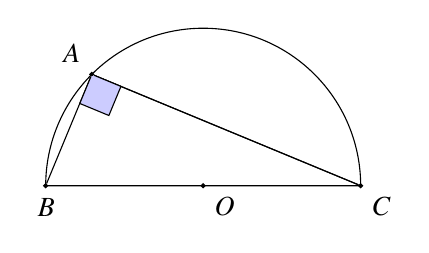
\begin{tikzpicture}
  [
    scale=2,
    >=stealth,
    point/.style = {draw, circle,  fill = black, inner sep = 0.5pt},
    dot/.style   = {draw, circle,  fill = black, inner sep = .2pt},
  ]

 \coordinate [point, label={below :	$B$ }] (B) at (-1, 0);
 \coordinate [point, label={below right:	$O$ }] (O) at (0, 0);
 \coordinate [point, label={below right:	$C$ }] (C) at (1, 0); 
 \coordinate [point, label={above left:	$A$ }] (A) at (-0.707,0.707);  
\draw (A) -- (C) arc(0:180:1) --cycle;
  \draw 
  (A) -- (B)
  (A) -- (C);
  \tkzMarkRightAngle[fill=blue!20,size=.2](B,A,C)    
%  \def\rad{1}

%  \draw (O) circle (\rad);  
%    \node (A) at +(45:{\rad}) [point,label = above right:$A$ $\brak{x,y}$] {};  
%  \path
%     (O)    edge  node[sloped, anchor=center, below, text width=0.5cm] { $r$}     (A) ; 
    
% \coordinate [point, label={below left:$B$}] (B) at (0, 0);
%    \node (A) at +(60:{2*sqrt(3)}) [label = above:$A$] {};
%  \coordinate [ label={below right:$C$ }] (C) at ($ (3,0) + sqrt(3)*(1,0) $);
%    \node (P) at +(30:{2*sqrt(3)}) [label = above:$P$] {};  
%  \path[->]
%     (B)    edge  node[sloped, anchor=center, below, text width=2.0cm] { $y = m_1x+c_1$}     (A) 
%	 (B)    edge  node[sloped, anchor=east, below, text width=2.0cm] { $y=m_2x+c_2$}     (C)
%	 (B)    edge  node[sloped, anchor=east, below, text width=2.0cm] { Bisector}     (P);
%  
%%  
%%  \coordinate [point, label={below left:$B$ $\brak{0,0}$}] (B) at (0, 0);
%%    \node (A) at +(60:{2*sqrt(3)}) [point, label = above:$A$ $\brak{a,b}$] {};
%%  \coordinate [point, label={below right:$C$ $\brak{c,0}$}] (C) at ($ (3,0) + sqrt(3)*(1,0) $);
%%  \node (D) at ({sqrt(3)},0) [point, label = below:$D$ $\brak{a,0}$] {};
%%    \node (E) at +(45:{(3+sqrt(3))/sqrt(2)}) [point, label = above right:$E$] {};
%%    \node (O) at +(45:{sqrt(6)}) [point, label = right:$O$] {};    
%%    \node (F) at +(60:{(3+sqrt(3))/2}) [point, label = left:$F$] {};        
%  \draw  (A) -- (B) -- (C);% -- (A);
%%  \node (D) at ($(B)!0.5!(C)$) [point, label = {below:$D$}]{};
%%  \draw (A) -- (D);  
%%  \draw (B) -- (E);    
%%  \draw[dashed] (C) -- (F);      
%\tkzMarkAngle[draw = black, fill = white, opacity=1](P,B,A)
%\tkzLabelAngle[pos = 0.8](P,B,A){$\theta$}
%\tkzMarkAngle[draw = black, fill = white, opacity=1,size=1.1](C,B,P)
%\tkzLabelAngle[pos = 0.9](C,B,P){$\theta$}

%\tkzMarkAngle[size=1.4,draw = black, fill = white, opacity=1](C,B,P)
%\tkzLabelAngle[pos=1.15,font=\scriptsize](C,B,P){$\theta$}

%  \tkzMarkAngle[fill=white,opacity=1,size=0.2,label={$\theta$},pos=0.2](P,B,A)  
%  \tkzMarkAngle[fill=blue!20,size=.4,label={$\theta$}](P,B,A)
%  \tkzMarkAngle[fill=blue!20,size=.2,label={$\theta$](C,B,P)
%  \tkzMarkRightAngle[fill=blue!20,size=.2](B,E,A)  
%  \path
%     (B)    edge  node[sloped, anchor=center, below, text width=2.0cm] { $k_1:1$}     (E)  
%	 (C)    edge  node[sloped, anchor=east, below, text width=2.0cm] { $1:k_2$}     (F);

\end{tikzpicture}


}
\caption{Angle in a semi-circle.}
\label{fig:ch2_line}
\end{figure}
\\
\solution Let 
\begin{align}
\vec{O} = 0
\end{align}
From the given information,
\begin{align}
\label{eq:semi_circ_pt}
\norm{\vec{A}}^2 = \norm{\vec{B}}^2 = \norm{\vec{C}}^2 = r^2
\\
\norm{\vec{B}-\vec{C}}^2 =  \brak{2r}^2
\\
\vec{B} + \vec{C} = 0
\label{eq:semcirc_mid}
\end{align}
%
where $r$ is the radius of the circle. Thus,
\begin{multline}
\norm{\vec{A}-\vec{B}}^2 + \norm{\vec{A}-\vec{C}}^2 = 
2\norm{\vec{A}}^2 + \norm{\vec{B}}^2 + \norm{\vec{C}}^2
\\
-2\vec{A}^T\brak{\vec{B}+\vec{C}}
%\\
%\norm{\vec{B}-\vec{C}}^2 =  \brak{2r}^2
%\\
%\vec{B} + \vec{C} = 0
\end{multline}
From \eqref{eq:semcirc_mid} and \eqref{eq:semi_circ_pt},
\begin{multline}
\norm{\vec{A}-\vec{B}}^2 + \norm{\vec{A}-\vec{C}}^2 = 4r^2 = \norm{\vec{B}-\vec{C}}^2 
%\\
%\norm{\vec{B}-\vec{C}}^2 =  \brak{2r}^2
%\\
%\vec{B} + \vec{C} = 0
\end{multline}
Thus, using Baudhayana's theorem, $\triangle ABC$ is right angled.
\item 	Show that $PA.PB = PC^2$, where $PC$ is the tangent to the circle in Fig. \ref{fig:tangent_secant}.

	\begin{figure}[!hb]
		\begin{center}
			
			%\includegraphics[width=\columnwidth]{./figs/ch4_tangent_prod}
			%\vspace*{-10cm}
			\resizebox{\columnwidth}{!}{\begin{tikzpicture}
[scale =2,>=stealth,point/.style = {draw, circle, fill = black, inner sep = 1pt},]

\def\rad{2}
\coordinate [point, label={above: $O$ }] (O) at (0, 2);
\draw (O) circle (\rad);
\node (P) at (-4,0)[point,label=below :$P$] {};
\node (C) at (0,0)[point,label=below :$C$] {};
\node (A) at (-1.92,1.45)[point,label=above left :$A$] {};
\node (B) at (1.2,3.6)[point,label=above right :$B$] {};
\draw (O)--(P);
\draw (P)--(C);
\draw (P)--(B);
%\draw (A)--(O);
%\draw (B)--(C);

\draw [thick,dashed](A)--(O);
\draw [thick,dashed](C)--(O);
\draw [thick,dashed](B)--(O);
%\tkzMarkRightAngle[size=.2](P,C,O);
%\tkzMarkAngle[size=.3](A,B,C);
%\tkzMarkAngle[size=.4](O,C,A);
%\tkzMarkAngle[size=.5](B,C,O);
%\tkzMarkAngle[size=.3](P,A,C);
%\tkzMarkAngle[size=.2](C,A,O);
%\tkzMarkAngle[size=.2](A,O,C);
%
\node [above] at (0.35,2.5){$r$};
\node [above] at (-0.9,1.7){$r$};
\node [above] at (0.1,1.0){$r$};
%\draw (-1.9,1) node{$\theta$};

%\draw (0.95,3.3) node{$\alpha$};
%\draw (-0.2,1.7) node{$2\alpha$};
%\draw (-0.2,0.5) node{$90-\alpha$};
%\draw (-1.4,1.4) node{$90-\alpha$};
%\draw (.1,.6) node{$\phi$};

\end{tikzpicture}}
		\end{center}
		\caption{$PA.PB = PC^2$.}
		\label{fig:tangent_secant}	
	\end{figure}
\solution Let $\vec{P} = \mbf{0}$.  Then, we have the following equations
\begin{align}
\label{eq:tan_sec_AB}
PA.PB &= \lambda \norm{\vec{A}}^2 \quad \because (\vec{B} = \lambda \vec{A})
\\
\norm{\vec{A}-\vec{O}}^2 &= \norm{\vec{B}-\vec{O}}^2 = \norm{\vec{C}-\vec{O}}^2 = r^2
\\
\norm{\vec{O}}^2-\norm{\vec{C}}^2 &=  r^2 \quad \triangle PCO\text{ is 
right angled}
\label{eq:tan_sec_boudh}
\end{align}
$\because$
\begin{align}
%\label{eq:tan_sec_AB}
%PA.PB &= \lambda \norm{\vec{A}}^2 \quad \because (\vec{B} = \lambda 
%\vec{A})
%\\
\norm{\vec{B}-\vec{O}}^2-\norm{\vec{A}-\vec{O}}^2   &=0,
\\
\brak{\lambda^2-1}\norm{\vec{A}}^2 - 2 \brak{\lambda-1}\vec{A}^T\vec{O} &= 
0
\\
\implies PA.PB = \lambda\norm{\vec{A}}^2 =  2 
\vec{A}^T\vec{O}-\norm{\vec{A}}^2 &
%\norm{\vec{C}-\vec{O}}^2 = r^2
%\\
%\norm{\vec{O}}^2-\norm{\vec{C}}^2 &=  r^2 \quad \triangle PCO\text{ is 
%right angled}
%\label{eq:tan_sec_boudh}
\label{eq:tan_sec_first}
\end{align}
after substituting from \eqref{eq:tan_sec_AB} and simplifying. From 
\eqref{eq:tan_sec_boudh},
\begin{align}
\norm{\vec{A}-\vec{O}}^2 = \norm{\vec{O}}^2-\norm{\vec{C}}^2  &= r^2
\\
\implies 2 \vec{A}^T\vec{O}-\norm{\vec{A}}^2   = \norm{\vec{C}}^2 = PC^2&
\label{eq:tan_sec_second}
\end{align}
From \eqref{eq:tan_sec_first} and \eqref{eq:tan_sec_second},
\begin{align}
PA.PB = PC^2
\end{align}

\item In Fig. \ref{fig:chords} show that $PA.PB = PC.PD$.
\begin{figure}[!ht]
	\begin{center}
		
		%\includegraphics[width=\columnwidth]{./figs/ch3_angle_bisector}
		%\vspace*{-10cm}
		\resizebox{\columnwidth}{!}{\begin{tikzpicture}
[scale=2,>=stealth,point/.style={draw,circle,fill = black,inner sep=0.5pt},]
%\node (D) at (0, 0)[point,label=below :$D$] {};
\node (B) at (-2, -2)[point,label=below left :$C$]{};
\node (A) at (1, 3)[point,label=above:$A$]{};
\node (C) at (4, -1)[point,label=below right:$B$]{};
%\coordinate [point, label={above : $O$ }] (I) at  (1.147, 1.143);
\node (O) at (0.7962963,-0.27777778)[point,label=above:$O$]{};
\node (D) at (  3.64041158, 1.36427295)[point,label=below:$D$]{};
\node (P) at ( 2.66371481, 0.78171359)[point,label=right:$P$]{};
%\node (x1) at (0.601,-1.357)[point,label=left:$x_1$]{};
%\node (x2) at (2.15,-1.1)[point,label=right:$x_2$]{};
%\node (temp) at ($(O)!0.5!(D)$)[label=right:$r$]{};
%\node (D) at (2.424,1.1)[point,label=above right:$D$]{};
%\node (E) at (1.1, 1.9)[point,label=above right:$E$]{};
%\node (F) at (-1.1, 1.9)[point,label=above left:$F$]{};
\def\rad{3.284101453883}
\draw (O) circle (\rad);

%\draw (D)--(O);
%\draw (A)--(B);
\draw (B)--(D);
\draw (A)--(C);
%\draw (C)--(D);
%\draw [thick,dashed] (x1) -- (x2);
%\draw [thick,dashed] (O) -- (E);
%\draw [thick,dashed] (O) -- (F);
%\draw (B)--(O);
%\draw (C)--(O);

%\tkzMarkRightAngle[size=.2](A,D,C)
%\tkzMarkRightAngle[size=.15](B,F,O);
%\tkzMarkRightAngle[size=.15](C,E,O);
%\tkzMarkAngle[size=.4](D,B,O);
%\tkzMarkAngle[size=.35](O,B,F);
%\tkzMarkAngle[size=.54](E,C,O);
%\tkzMarkAngle[size=.5](E,C,O);
%\tkzMarkAngle[size=.6](O,C,D);
%\tkzMarkAngle[size=.65](O,C,D);

\end{tikzpicture}}
	\end{center}
	\caption{Chords of a circle}
	\label{fig:chords}	
\end{figure}
\\
\solution Let $\vec{P} = \mbf{0}$.  We then have the following equations
\begin{align}
\begin{split}
\vec{B} &= k_1 \vec{A}, k_1 = \frac{PB}{PA}
\\
\vec{D} &= k_2 \vec{C}, k_2 = \frac{PD}{PC}
\end{split}
\label{eq:chords_ratio}
\\
\begin{split}
\norm{\vec{A}-\vec{O}}^2 &= \norm{\vec{B}-\vec{O}}^2 
\\
= \norm{\vec{C}-\vec{O}}^2 &= \norm{\vec{D}-\vec{O}}^2 = r^2
\end{split}
\label{eq:chords_points}
\end{align}
%
where $r$ is the radius of the circle and $\vec{O}$ is the centre. From \eqref{eq:chords_points},
\begin{align}
&\norm{\vec{A}-\vec{O}}^2 = \norm{\vec{B}-\vec{O}}^2
\\
\implies &\norm{\vec{A}-\vec{O}}^2 = \norm{k\vec{A}-\vec{O}}^2 \quad(\text{from \eqref{eq:chords_ratio}})
\end{align}
%
which can be simplified to obtain
\begin{align}
k_1\norm{\vec{A}}^2 = 2\vec{A}^T\vec{O}-\norm{\vec{A}}^2
\label{eq:chords_Anorm}
\end{align}
Similarly,
\begin{align}
k_2\norm{\vec{C}}^2 = 2\vec{C}^T\vec{O}-\norm{\vec{C}}^2
\label{eq:chords_Cnorm}
\end{align}
%
From \eqref{eq:chords_points}, we also obtain
\begin{align}
\norm{\vec{A}-\vec{O}}^2 
= \norm{\vec{C}-\vec{O}}^2 
\\
\implies 2\vec{A}^T\vec{O}-\norm{\vec{A}}^2 = 2\vec{C}^T\vec{O}-\norm{\vec{C}}^2
\label{eq:chords_ACnorm}
\end{align}
%
after simplification. Using this result in \eqref{eq:chords_Anorm} and \eqref{eq:chords_Cnorm},
\begin{align}
k_1\norm{\vec{A}}^2 = k_2\norm{\vec{C}}^2
\\
\implies \norm{\vec{A}}\, \norm{\vec{B}}=\norm{\vec{C}}\,\norm{\vec{D}}
\end{align}
which completes the proof.

\item (Pole and Polar:) The polar of a point $\vec{x}$ with respect to the curve
\begin{align}
\label{eq:quad_form_polar}
\vec{x}^T\vec{V}\vec{x}+2\vec{u}^T\vec{x}+f=0
\end{align}
is the line
\begin{align}
\label{eq:polar}
\vec{n}^T\vec{x} = c
\end{align}
%
where
\begin{align}
\myvec{\vec{n}^T\\ - c}=
\myvec{
\vec{V}&\vec{u}
\\
\vec{u}^T&f
}
\myvec{\vec{x}\\1}
\end{align}
%
The pole of the line  in \eqref{eq:polar} is obtained as $\frac{1}{x_3}\myvec{x_1\\x_2}$, where
\begin{align}
\myvec{x_1 \\ x_2\\x_3}
=\myvec{
\vec{V}&\vec{u}
\\
\vec{u}^T&f
}^{-1}
\myvec{\vec{n}^T\\ - c}
\end{align}
\item $\vec{x}_1$ and $\vec{x}_2$ are said to be conjugate points for \eqref{eq:quad_form_polar} if $\vec{x}_2$ lies on the polar of $\vec{x}_1$ and vice-versa.  A similar definition holds for conjugate lines as well.
\item Let $\vec{p}$ be a point of intersection of two circles with centres $\vec{c}_1$ and $\vec{c}_2$.  The circles are said to be orthogonal if their tangents at $\vec{p}$ are perpendicular to each other.  Show that if $r_1$ and $r_2$ are their respective radii, 
\begin{align}
\label{eq:circ_orth}
\norm{\vec{c_1}-\vec{c}_2}^2 = r_1^2+r_2^2 
\end{align}
\item Show that the length of the tangent from a point $\vec{p}$ to the circle 
\begin{align}
\label{eq:circ_quad_len}
\vec{x}^T\vec{x}-2\vec{c}^T\vec{x} + f = 0
\end{align}
%
is 
\begin{align}
\label{eq:circ_tang_len}
\vec{p}^T\vec{p}-2\vec{c}^T\vec{p} + f 
\end{align}
This length is also known as the {\em power} of the point $\vec{p}$ with respect to the circle.
\item  The {\em radical axis} of the circles 
\begin{align}
%\label{eq:circs_two}
\vec{x}^T\vec{x}-2\vec{c}_1^T\vec{x} + f_1 = 0
\\
\vec{x}^T\vec{x}-2\vec{c}_2^T\vec{x} + f_2 = 0
\end{align}
%
is the locus of the points from which lengths of the tangents to the circles are equal.  From \eqref{eq:circs_two}, this locus is
\begin{align}
\vec{x}^T\vec{x}-2\vec{c}_1^T\vec{x} + f_1 -
%\nonumber \\
\vec{x}^T\vec{x}-2\vec{c}_2^T\vec{x} + f_2 = 0
\\
\implies 2\brak{\vec{c}_1-\vec{c}_2}^T\vec{x} + f_2 - f_1 = 0
\label{eq:circs_rad_axis}
\end{align}
\item Show that the radical axis of the circles is perpendicular to the line joining their centres.\item {\em Coaxal circles} have the same radical axis.
\item Obtain a family of coaxal circles from \label{eq:circs_two} and find their {\em limit points}.
\\
\solution The family of circles is obtained as
\begin{align}
\label{eq:circs_coaxal_family}
\vec{x}^T\vec{x}-2\brak{\vec{c}_1 +\lambda\vec{c}_2}^T\vec{x} + f_1 +\lambda f_2= 0
\end{align}
%
The limit points are the centres of those circles whose radii are 0. From \eqref{eq:circs_coaxal_family} and \eqref{eq:circ_quad},
this results in
\begin{align}
%\label{eq:circs_coaxal_family}
f_1 +\lambda f_2 =  \brak{\vec{c}_1 +\lambda\vec{c}_2}^T\brak{\vec{c}_1 +\lambda\vec{c}_2} &
\\
\implies \lambda^2 \norm{\vec{c}_2}^2 + \lambda \brak{2\vec{c}_1^T\vec{c}_2-f_2} + \norm{\vec{c}_1}^2-f_1 = 0&
\end{align}
Solving for $\lambda$, the limit points are given by  
\begin{align}
\vec{c}_1+\lambda\vec{c}_2
\end{align}
\end{enumerate}


 
\subsection{Equation}
\renewcommand{\theequation}{\theenumi}
\begin{enumerate}[label=\arabic*.,ref=\thesubsection.\theenumi]
\item Find the radius and the coordinates of the centre of each of the following circles:
\begin{enumerate}
\item
$
3\vec{x}^T\vec{x}+\myvec{-12 & 6}\vec{x} + 11 = 0
%3x^2+3y^2-12x+6y+11 = 0
$
\\
\solution
Let the balanced version of (\ref{eq:solutions/chem/6ato balance}) be
\begin{align}
    \label{eq:solutions/chem/6abalanced}x_{1}HNO_{3}+ x_{2}Ca(OH)_{2}\to x_{3}Ca(NO_{3})_{2}+ x_{4}H_{2}O
\end{align}

which results in the following equations:
\begin{align}
    (x_{1}+ 2x_{2}-2x_{4}) H= 0\\
    (x_{1}-2x_{3}) N= 0\\
    (3x_{1}+ 2x_{2}-6x_{3}- x_{4}) O=0\\
    (x_{2}-x_{3}) Ca= 0
\end{align}

which can be expressed as
\begin{align}
    x_{1}+ 2x_{2}+ 0.x_{3} -2x_{4} = 0\\
    x_{1}+ 0.x_{2} -2x_{3} +0.x_{4}= 0\\
    3x_{1}+ 2x_{2}-6x_{3}- x_{4} =0\\
    0.x_{1} +x_{2}-x_{3} +0.x_{4}= 0
\end{align}

resulting in the matrix equation
\begin{align}
    \label{eq:solutions/chem/6a matrix}
    \myvec{1 & 2 & 0 & -2\\
           1 & 0 & -2 & 0\\
           3 & 2 & -6 & -1\\
           0 & 1 & -1 & 0}\vec{x}
           =\vec{0}
\end{align}

where,
\begin{align}
   \vec{x}= \myvec{x_{1}\\x_{2}\\x_{3}\\x_{4}}
\end{align}

(\ref{eq:solutions/chem/6a matrix}) can be reduced as follows:
\begin{align}
    \myvec{1 & 2 & 0 & -2\\
           1 & 0 & -2 & 0\\
           3 & 2 & -6 & -1\\
           0 & 1 & -1 & 0}
    \xleftrightarrow[R_{3}\leftarrow \frac{R_3}{3}-R_{1}]{R_{2}\leftarrow R_2- R_1}
    \myvec{1 & 2 & 0 & -2\\
           0 & -2 & -2 & 2\\
           0 & -\frac{4}{3} & -2 & \frac{5}{3}\\
           0 & 1 & -1 & 0}\\
    \xleftrightarrow{R_2 \leftarrow -\frac{R_2}{2}}
    \myvec{1 & 2 & 0 & -2\\
          0 & 1 & 1 & -1\\
          0 & -\frac{4}{3} & -2 & \frac{5}{3}\\
          0 & 1 & -1 & 0}\\
    \xleftrightarrow[R_4 \leftarrow R_4- R_2]{R_3 \leftarrow R_3 + \frac{4}{3}R_2}
    \myvec{1 & 2 & 0 & -2\\
           0 & 1 & 1 & -1\\
           0 & 0 & -\frac{2}{3} & \frac{1}{3}\\
           0 & 0 & -2 & 1}\\
    \xleftrightarrow[R_3 \leftarrow -\frac{3}{2}R_3]{R_1 \leftarrow R_1- 2R_2}
    \myvec{1 & 0 & -2 & 0\\
           0 & 1 & 1 & -1\\
           0 & 0 & 1 & -\frac{1}{2}\\
           0 & 0 & -2 & 1}\\
    \xleftrightarrow{R_4\leftarrow R_4 + 2R_3}
    \myvec{1 & 0 & -2 & 0\\
           0 & 1 & 1 & -1\\
           0 & 0 & 1 & -\frac{1}{2}\\
           0 & 0 & 0 & 0}\\
    \xleftrightarrow[R_2\leftarrow R_2-R_3]{R_1\leftarrow R_1 + 2R_3}
    \myvec{1 & 0 & 0 & -1\\
           0 & 1 & 0 & -\frac{1}{2}\\
           0 & 0 & 1 & -\frac{1}{2}\\
           0 & 0 & 0 & 0}
\end{align}

Thus,
\begin{align}
    x_1=x_4, x_2= \frac{1}{2}x_4, x_3=\frac{1}{2}x_4\\
    \implies \quad\vec{x}= x_4\myvec{1\\ \frac{1}{2}\\ \frac{1}{2}\\1} =\myvec{2\\1\\1\\2}
\end{align} 
by substituting $x_4= 2$.

\hfill\break
%\vspace{5mm} 
Hence, (\ref{eq:solutions/chem/6abalanced}) finally becomes
\begin{align}
    2HNO_{3}+ Ca(OH)_{2}\to Ca(NO_{3})_{2}+ 2H_{2}O
\end{align}

\item
$
\vec{x}^T\vec{x} = a^2+b^2
$
\item
$
2\vec{x}^T\vec{x}+\myvec{16 & -4}\vec{x}+33 = 0
%2x^2+2y^2+16x-4y+88 = 0
$
\item
$
36\vec{x}^T\vec{x}-\myvec{36 & 24}\vec{x}-131=0
%36x^2+36y^2-36x-24y-131 = 0
$
\end{enumerate}
\item Find the equation of the circle that passes through the points $\myvec{1\\2}$, $\myvec{2\\1}$, $\myvec{0\\0}$.
\\
\solution
Let the balanced version of (\ref{eq:solutions/chem/6ato balance}) be
\begin{align}
    \label{eq:solutions/chem/6abalanced}x_{1}HNO_{3}+ x_{2}Ca(OH)_{2}\to x_{3}Ca(NO_{3})_{2}+ x_{4}H_{2}O
\end{align}

which results in the following equations:
\begin{align}
    (x_{1}+ 2x_{2}-2x_{4}) H= 0\\
    (x_{1}-2x_{3}) N= 0\\
    (3x_{1}+ 2x_{2}-6x_{3}- x_{4}) O=0\\
    (x_{2}-x_{3}) Ca= 0
\end{align}

which can be expressed as
\begin{align}
    x_{1}+ 2x_{2}+ 0.x_{3} -2x_{4} = 0\\
    x_{1}+ 0.x_{2} -2x_{3} +0.x_{4}= 0\\
    3x_{1}+ 2x_{2}-6x_{3}- x_{4} =0\\
    0.x_{1} +x_{2}-x_{3} +0.x_{4}= 0
\end{align}

resulting in the matrix equation
\begin{align}
    \label{eq:solutions/chem/6a matrix}
    \myvec{1 & 2 & 0 & -2\\
           1 & 0 & -2 & 0\\
           3 & 2 & -6 & -1\\
           0 & 1 & -1 & 0}\vec{x}
           =\vec{0}
\end{align}

where,
\begin{align}
   \vec{x}= \myvec{x_{1}\\x_{2}\\x_{3}\\x_{4}}
\end{align}

(\ref{eq:solutions/chem/6a matrix}) can be reduced as follows:
\begin{align}
    \myvec{1 & 2 & 0 & -2\\
           1 & 0 & -2 & 0\\
           3 & 2 & -6 & -1\\
           0 & 1 & -1 & 0}
    \xleftrightarrow[R_{3}\leftarrow \frac{R_3}{3}-R_{1}]{R_{2}\leftarrow R_2- R_1}
    \myvec{1 & 2 & 0 & -2\\
           0 & -2 & -2 & 2\\
           0 & -\frac{4}{3} & -2 & \frac{5}{3}\\
           0 & 1 & -1 & 0}\\
    \xleftrightarrow{R_2 \leftarrow -\frac{R_2}{2}}
    \myvec{1 & 2 & 0 & -2\\
          0 & 1 & 1 & -1\\
          0 & -\frac{4}{3} & -2 & \frac{5}{3}\\
          0 & 1 & -1 & 0}\\
    \xleftrightarrow[R_4 \leftarrow R_4- R_2]{R_3 \leftarrow R_3 + \frac{4}{3}R_2}
    \myvec{1 & 2 & 0 & -2\\
           0 & 1 & 1 & -1\\
           0 & 0 & -\frac{2}{3} & \frac{1}{3}\\
           0 & 0 & -2 & 1}\\
    \xleftrightarrow[R_3 \leftarrow -\frac{3}{2}R_3]{R_1 \leftarrow R_1- 2R_2}
    \myvec{1 & 0 & -2 & 0\\
           0 & 1 & 1 & -1\\
           0 & 0 & 1 & -\frac{1}{2}\\
           0 & 0 & -2 & 1}\\
    \xleftrightarrow{R_4\leftarrow R_4 + 2R_3}
    \myvec{1 & 0 & -2 & 0\\
           0 & 1 & 1 & -1\\
           0 & 0 & 1 & -\frac{1}{2}\\
           0 & 0 & 0 & 0}\\
    \xleftrightarrow[R_2\leftarrow R_2-R_3]{R_1\leftarrow R_1 + 2R_3}
    \myvec{1 & 0 & 0 & -1\\
           0 & 1 & 0 & -\frac{1}{2}\\
           0 & 0 & 1 & -\frac{1}{2}\\
           0 & 0 & 0 & 0}
\end{align}

Thus,
\begin{align}
    x_1=x_4, x_2= \frac{1}{2}x_4, x_3=\frac{1}{2}x_4\\
    \implies \quad\vec{x}= x_4\myvec{1\\ \frac{1}{2}\\ \frac{1}{2}\\1} =\myvec{2\\1\\1\\2}
\end{align} 
by substituting $x_4= 2$.

\hfill\break
%\vspace{5mm} 
Hence, (\ref{eq:solutions/chem/6abalanced}) finally becomes
\begin{align}
    2HNO_{3}+ Ca(OH)_{2}\to Ca(NO_{3})_{2}+ 2H_{2}O
\end{align}

\item Find the equation of the circle that passes through  the points $\myvec{2\\3}$, $\myvec{3\\2}$, $\myvec{5\\1}$.
\\
\solution
Let the balanced version of (\ref{eq:solutions/chem/6ato balance}) be
\begin{align}
    \label{eq:solutions/chem/6abalanced}x_{1}HNO_{3}+ x_{2}Ca(OH)_{2}\to x_{3}Ca(NO_{3})_{2}+ x_{4}H_{2}O
\end{align}

which results in the following equations:
\begin{align}
    (x_{1}+ 2x_{2}-2x_{4}) H= 0\\
    (x_{1}-2x_{3}) N= 0\\
    (3x_{1}+ 2x_{2}-6x_{3}- x_{4}) O=0\\
    (x_{2}-x_{3}) Ca= 0
\end{align}

which can be expressed as
\begin{align}
    x_{1}+ 2x_{2}+ 0.x_{3} -2x_{4} = 0\\
    x_{1}+ 0.x_{2} -2x_{3} +0.x_{4}= 0\\
    3x_{1}+ 2x_{2}-6x_{3}- x_{4} =0\\
    0.x_{1} +x_{2}-x_{3} +0.x_{4}= 0
\end{align}

resulting in the matrix equation
\begin{align}
    \label{eq:solutions/chem/6a matrix}
    \myvec{1 & 2 & 0 & -2\\
           1 & 0 & -2 & 0\\
           3 & 2 & -6 & -1\\
           0 & 1 & -1 & 0}\vec{x}
           =\vec{0}
\end{align}

where,
\begin{align}
   \vec{x}= \myvec{x_{1}\\x_{2}\\x_{3}\\x_{4}}
\end{align}

(\ref{eq:solutions/chem/6a matrix}) can be reduced as follows:
\begin{align}
    \myvec{1 & 2 & 0 & -2\\
           1 & 0 & -2 & 0\\
           3 & 2 & -6 & -1\\
           0 & 1 & -1 & 0}
    \xleftrightarrow[R_{3}\leftarrow \frac{R_3}{3}-R_{1}]{R_{2}\leftarrow R_2- R_1}
    \myvec{1 & 2 & 0 & -2\\
           0 & -2 & -2 & 2\\
           0 & -\frac{4}{3} & -2 & \frac{5}{3}\\
           0 & 1 & -1 & 0}\\
    \xleftrightarrow{R_2 \leftarrow -\frac{R_2}{2}}
    \myvec{1 & 2 & 0 & -2\\
          0 & 1 & 1 & -1\\
          0 & -\frac{4}{3} & -2 & \frac{5}{3}\\
          0 & 1 & -1 & 0}\\
    \xleftrightarrow[R_4 \leftarrow R_4- R_2]{R_3 \leftarrow R_3 + \frac{4}{3}R_2}
    \myvec{1 & 2 & 0 & -2\\
           0 & 1 & 1 & -1\\
           0 & 0 & -\frac{2}{3} & \frac{1}{3}\\
           0 & 0 & -2 & 1}\\
    \xleftrightarrow[R_3 \leftarrow -\frac{3}{2}R_3]{R_1 \leftarrow R_1- 2R_2}
    \myvec{1 & 0 & -2 & 0\\
           0 & 1 & 1 & -1\\
           0 & 0 & 1 & -\frac{1}{2}\\
           0 & 0 & -2 & 1}\\
    \xleftrightarrow{R_4\leftarrow R_4 + 2R_3}
    \myvec{1 & 0 & -2 & 0\\
           0 & 1 & 1 & -1\\
           0 & 0 & 1 & -\frac{1}{2}\\
           0 & 0 & 0 & 0}\\
    \xleftrightarrow[R_2\leftarrow R_2-R_3]{R_1\leftarrow R_1 + 2R_3}
    \myvec{1 & 0 & 0 & -1\\
           0 & 1 & 0 & -\frac{1}{2}\\
           0 & 0 & 1 & -\frac{1}{2}\\
           0 & 0 & 0 & 0}
\end{align}

Thus,
\begin{align}
    x_1=x_4, x_2= \frac{1}{2}x_4, x_3=\frac{1}{2}x_4\\
    \implies \quad\vec{x}= x_4\myvec{1\\ \frac{1}{2}\\ \frac{1}{2}\\1} =\myvec{2\\1\\1\\2}
\end{align} 
by substituting $x_4= 2$.

\hfill\break
%\vspace{5mm} 
Hence, (\ref{eq:solutions/chem/6abalanced}) finally becomes
\begin{align}
    2HNO_{3}+ Ca(OH)_{2}\to Ca(NO_{3})_{2}+ 2H_{2}O
\end{align}

\item Find the equation of the circle that passes through the points $\myvec{2a\\0}$, $\myvec{0\\2b}$, $\myvec{a+b\\a+b}$.
\\
\solution
Let the balanced version of (\ref{eq:solutions/chem/6ato balance}) be
\begin{align}
    \label{eq:solutions/chem/6abalanced}x_{1}HNO_{3}+ x_{2}Ca(OH)_{2}\to x_{3}Ca(NO_{3})_{2}+ x_{4}H_{2}O
\end{align}

which results in the following equations:
\begin{align}
    (x_{1}+ 2x_{2}-2x_{4}) H= 0\\
    (x_{1}-2x_{3}) N= 0\\
    (3x_{1}+ 2x_{2}-6x_{3}- x_{4}) O=0\\
    (x_{2}-x_{3}) Ca= 0
\end{align}

which can be expressed as
\begin{align}
    x_{1}+ 2x_{2}+ 0.x_{3} -2x_{4} = 0\\
    x_{1}+ 0.x_{2} -2x_{3} +0.x_{4}= 0\\
    3x_{1}+ 2x_{2}-6x_{3}- x_{4} =0\\
    0.x_{1} +x_{2}-x_{3} +0.x_{4}= 0
\end{align}

resulting in the matrix equation
\begin{align}
    \label{eq:solutions/chem/6a matrix}
    \myvec{1 & 2 & 0 & -2\\
           1 & 0 & -2 & 0\\
           3 & 2 & -6 & -1\\
           0 & 1 & -1 & 0}\vec{x}
           =\vec{0}
\end{align}

where,
\begin{align}
   \vec{x}= \myvec{x_{1}\\x_{2}\\x_{3}\\x_{4}}
\end{align}

(\ref{eq:solutions/chem/6a matrix}) can be reduced as follows:
\begin{align}
    \myvec{1 & 2 & 0 & -2\\
           1 & 0 & -2 & 0\\
           3 & 2 & -6 & -1\\
           0 & 1 & -1 & 0}
    \xleftrightarrow[R_{3}\leftarrow \frac{R_3}{3}-R_{1}]{R_{2}\leftarrow R_2- R_1}
    \myvec{1 & 2 & 0 & -2\\
           0 & -2 & -2 & 2\\
           0 & -\frac{4}{3} & -2 & \frac{5}{3}\\
           0 & 1 & -1 & 0}\\
    \xleftrightarrow{R_2 \leftarrow -\frac{R_2}{2}}
    \myvec{1 & 2 & 0 & -2\\
          0 & 1 & 1 & -1\\
          0 & -\frac{4}{3} & -2 & \frac{5}{3}\\
          0 & 1 & -1 & 0}\\
    \xleftrightarrow[R_4 \leftarrow R_4- R_2]{R_3 \leftarrow R_3 + \frac{4}{3}R_2}
    \myvec{1 & 2 & 0 & -2\\
           0 & 1 & 1 & -1\\
           0 & 0 & -\frac{2}{3} & \frac{1}{3}\\
           0 & 0 & -2 & 1}\\
    \xleftrightarrow[R_3 \leftarrow -\frac{3}{2}R_3]{R_1 \leftarrow R_1- 2R_2}
    \myvec{1 & 0 & -2 & 0\\
           0 & 1 & 1 & -1\\
           0 & 0 & 1 & -\frac{1}{2}\\
           0 & 0 & -2 & 1}\\
    \xleftrightarrow{R_4\leftarrow R_4 + 2R_3}
    \myvec{1 & 0 & -2 & 0\\
           0 & 1 & 1 & -1\\
           0 & 0 & 1 & -\frac{1}{2}\\
           0 & 0 & 0 & 0}\\
    \xleftrightarrow[R_2\leftarrow R_2-R_3]{R_1\leftarrow R_1 + 2R_3}
    \myvec{1 & 0 & 0 & -1\\
           0 & 1 & 0 & -\frac{1}{2}\\
           0 & 0 & 1 & -\frac{1}{2}\\
           0 & 0 & 0 & 0}
\end{align}

Thus,
\begin{align}
    x_1=x_4, x_2= \frac{1}{2}x_4, x_3=\frac{1}{2}x_4\\
    \implies \quad\vec{x}= x_4\myvec{1\\ \frac{1}{2}\\ \frac{1}{2}\\1} =\myvec{2\\1\\1\\2}
\end{align} 
by substituting $x_4= 2$.

\hfill\break
%\vspace{5mm} 
Hence, (\ref{eq:solutions/chem/6abalanced}) finally becomes
\begin{align}
    2HNO_{3}+ Ca(OH)_{2}\to Ca(NO_{3})_{2}+ 2H_{2}O
\end{align}

\item A circle has its centre on the line $x=2y$ and passes through the points $\myvec{-1\\2}$, $\myvec{3\\-2}$.  Find the coordinates
of the centre and the equation of the circle.
\\
\solution
Let the balanced version of (\ref{eq:solutions/chem/6ato balance}) be
\begin{align}
    \label{eq:solutions/chem/6abalanced}x_{1}HNO_{3}+ x_{2}Ca(OH)_{2}\to x_{3}Ca(NO_{3})_{2}+ x_{4}H_{2}O
\end{align}

which results in the following equations:
\begin{align}
    (x_{1}+ 2x_{2}-2x_{4}) H= 0\\
    (x_{1}-2x_{3}) N= 0\\
    (3x_{1}+ 2x_{2}-6x_{3}- x_{4}) O=0\\
    (x_{2}-x_{3}) Ca= 0
\end{align}

which can be expressed as
\begin{align}
    x_{1}+ 2x_{2}+ 0.x_{3} -2x_{4} = 0\\
    x_{1}+ 0.x_{2} -2x_{3} +0.x_{4}= 0\\
    3x_{1}+ 2x_{2}-6x_{3}- x_{4} =0\\
    0.x_{1} +x_{2}-x_{3} +0.x_{4}= 0
\end{align}

resulting in the matrix equation
\begin{align}
    \label{eq:solutions/chem/6a matrix}
    \myvec{1 & 2 & 0 & -2\\
           1 & 0 & -2 & 0\\
           3 & 2 & -6 & -1\\
           0 & 1 & -1 & 0}\vec{x}
           =\vec{0}
\end{align}

where,
\begin{align}
   \vec{x}= \myvec{x_{1}\\x_{2}\\x_{3}\\x_{4}}
\end{align}

(\ref{eq:solutions/chem/6a matrix}) can be reduced as follows:
\begin{align}
    \myvec{1 & 2 & 0 & -2\\
           1 & 0 & -2 & 0\\
           3 & 2 & -6 & -1\\
           0 & 1 & -1 & 0}
    \xleftrightarrow[R_{3}\leftarrow \frac{R_3}{3}-R_{1}]{R_{2}\leftarrow R_2- R_1}
    \myvec{1 & 2 & 0 & -2\\
           0 & -2 & -2 & 2\\
           0 & -\frac{4}{3} & -2 & \frac{5}{3}\\
           0 & 1 & -1 & 0}\\
    \xleftrightarrow{R_2 \leftarrow -\frac{R_2}{2}}
    \myvec{1 & 2 & 0 & -2\\
          0 & 1 & 1 & -1\\
          0 & -\frac{4}{3} & -2 & \frac{5}{3}\\
          0 & 1 & -1 & 0}\\
    \xleftrightarrow[R_4 \leftarrow R_4- R_2]{R_3 \leftarrow R_3 + \frac{4}{3}R_2}
    \myvec{1 & 2 & 0 & -2\\
           0 & 1 & 1 & -1\\
           0 & 0 & -\frac{2}{3} & \frac{1}{3}\\
           0 & 0 & -2 & 1}\\
    \xleftrightarrow[R_3 \leftarrow -\frac{3}{2}R_3]{R_1 \leftarrow R_1- 2R_2}
    \myvec{1 & 0 & -2 & 0\\
           0 & 1 & 1 & -1\\
           0 & 0 & 1 & -\frac{1}{2}\\
           0 & 0 & -2 & 1}\\
    \xleftrightarrow{R_4\leftarrow R_4 + 2R_3}
    \myvec{1 & 0 & -2 & 0\\
           0 & 1 & 1 & -1\\
           0 & 0 & 1 & -\frac{1}{2}\\
           0 & 0 & 0 & 0}\\
    \xleftrightarrow[R_2\leftarrow R_2-R_3]{R_1\leftarrow R_1 + 2R_3}
    \myvec{1 & 0 & 0 & -1\\
           0 & 1 & 0 & -\frac{1}{2}\\
           0 & 0 & 1 & -\frac{1}{2}\\
           0 & 0 & 0 & 0}
\end{align}

Thus,
\begin{align}
    x_1=x_4, x_2= \frac{1}{2}x_4, x_3=\frac{1}{2}x_4\\
    \implies \quad\vec{x}= x_4\myvec{1\\ \frac{1}{2}\\ \frac{1}{2}\\1} =\myvec{2\\1\\1\\2}
\end{align} 
by substituting $x_4= 2$.

\hfill\break
%\vspace{5mm} 
Hence, (\ref{eq:solutions/chem/6abalanced}) finally becomes
\begin{align}
    2HNO_{3}+ Ca(OH)_{2}\to Ca(NO_{3})_{2}+ 2H_{2}O
\end{align}

\item Find the locus of the centre of a circle which touches the line 
\numberwithin{equation}{enumi}
\begin{align}
\myvec{\cos\alpha  & \sin\alpha}\vec{x} =p
\end{align}
 and the circle 
\begin{align}
\norm{\vec{x}-\vec{c}} = r
\end{align}
\end{enumerate}
 
\subsection{Tangent and Normal}
\renewcommand{\theequation}{\theenumi}
\begin{enumerate}[label=\arabic*.,ref=\thesubsection.\theenumi]
\numberwithin{equation}{enumi}
\item Without drawing a figure, determine whether the points $\myvec{-1\\2}$, $\myvec{0\\0}$, $\myvec{3\\-4}$ lie outside, on the circumference, or inside the circle
\begin{align}
\vec{x}^T\vec{x}+\myvec{-5 & 2}\vec{x}-5 = 0
\end{align}
\solution
Let the balanced version of (\ref{eq:solutions/chem/6ato balance}) be
\begin{align}
    \label{eq:solutions/chem/6abalanced}x_{1}HNO_{3}+ x_{2}Ca(OH)_{2}\to x_{3}Ca(NO_{3})_{2}+ x_{4}H_{2}O
\end{align}

which results in the following equations:
\begin{align}
    (x_{1}+ 2x_{2}-2x_{4}) H= 0\\
    (x_{1}-2x_{3}) N= 0\\
    (3x_{1}+ 2x_{2}-6x_{3}- x_{4}) O=0\\
    (x_{2}-x_{3}) Ca= 0
\end{align}

which can be expressed as
\begin{align}
    x_{1}+ 2x_{2}+ 0.x_{3} -2x_{4} = 0\\
    x_{1}+ 0.x_{2} -2x_{3} +0.x_{4}= 0\\
    3x_{1}+ 2x_{2}-6x_{3}- x_{4} =0\\
    0.x_{1} +x_{2}-x_{3} +0.x_{4}= 0
\end{align}

resulting in the matrix equation
\begin{align}
    \label{eq:solutions/chem/6a matrix}
    \myvec{1 & 2 & 0 & -2\\
           1 & 0 & -2 & 0\\
           3 & 2 & -6 & -1\\
           0 & 1 & -1 & 0}\vec{x}
           =\vec{0}
\end{align}

where,
\begin{align}
   \vec{x}= \myvec{x_{1}\\x_{2}\\x_{3}\\x_{4}}
\end{align}

(\ref{eq:solutions/chem/6a matrix}) can be reduced as follows:
\begin{align}
    \myvec{1 & 2 & 0 & -2\\
           1 & 0 & -2 & 0\\
           3 & 2 & -6 & -1\\
           0 & 1 & -1 & 0}
    \xleftrightarrow[R_{3}\leftarrow \frac{R_3}{3}-R_{1}]{R_{2}\leftarrow R_2- R_1}
    \myvec{1 & 2 & 0 & -2\\
           0 & -2 & -2 & 2\\
           0 & -\frac{4}{3} & -2 & \frac{5}{3}\\
           0 & 1 & -1 & 0}\\
    \xleftrightarrow{R_2 \leftarrow -\frac{R_2}{2}}
    \myvec{1 & 2 & 0 & -2\\
          0 & 1 & 1 & -1\\
          0 & -\frac{4}{3} & -2 & \frac{5}{3}\\
          0 & 1 & -1 & 0}\\
    \xleftrightarrow[R_4 \leftarrow R_4- R_2]{R_3 \leftarrow R_3 + \frac{4}{3}R_2}
    \myvec{1 & 2 & 0 & -2\\
           0 & 1 & 1 & -1\\
           0 & 0 & -\frac{2}{3} & \frac{1}{3}\\
           0 & 0 & -2 & 1}\\
    \xleftrightarrow[R_3 \leftarrow -\frac{3}{2}R_3]{R_1 \leftarrow R_1- 2R_2}
    \myvec{1 & 0 & -2 & 0\\
           0 & 1 & 1 & -1\\
           0 & 0 & 1 & -\frac{1}{2}\\
           0 & 0 & -2 & 1}\\
    \xleftrightarrow{R_4\leftarrow R_4 + 2R_3}
    \myvec{1 & 0 & -2 & 0\\
           0 & 1 & 1 & -1\\
           0 & 0 & 1 & -\frac{1}{2}\\
           0 & 0 & 0 & 0}\\
    \xleftrightarrow[R_2\leftarrow R_2-R_3]{R_1\leftarrow R_1 + 2R_3}
    \myvec{1 & 0 & 0 & -1\\
           0 & 1 & 0 & -\frac{1}{2}\\
           0 & 0 & 1 & -\frac{1}{2}\\
           0 & 0 & 0 & 0}
\end{align}

Thus,
\begin{align}
    x_1=x_4, x_2= \frac{1}{2}x_4, x_3=\frac{1}{2}x_4\\
    \implies \quad\vec{x}= x_4\myvec{1\\ \frac{1}{2}\\ \frac{1}{2}\\1} =\myvec{2\\1\\1\\2}
\end{align} 
by substituting $x_4= 2$.

\hfill\break
%\vspace{5mm} 
Hence, (\ref{eq:solutions/chem/6abalanced}) finally becomes
\begin{align}
    2HNO_{3}+ Ca(OH)_{2}\to Ca(NO_{3})_{2}+ 2H_{2}O
\end{align}

\item Find the points of intersection of the line
\begin{align}
    \label{eq:solutions/4/2/2/eq1}\myvec{3 & 2}\vec x = 12
\end{align}
and the circle
\begin{align}
    \label{eq:solutions/4/2/2/eq:circle} \norm{\vec{x}}^2 = 13
\end{align}
and for what values of $c$ the line
\begin{align}
    \label{eq:solutions/4/2/2/tangent}\myvec{3 &2}\vec x = c 
\end{align}
touches the circle.
\\
%
\solution
Let the balanced version of (\ref{eq:solutions/chem/6ato balance}) be
\begin{align}
    \label{eq:solutions/chem/6abalanced}x_{1}HNO_{3}+ x_{2}Ca(OH)_{2}\to x_{3}Ca(NO_{3})_{2}+ x_{4}H_{2}O
\end{align}

which results in the following equations:
\begin{align}
    (x_{1}+ 2x_{2}-2x_{4}) H= 0\\
    (x_{1}-2x_{3}) N= 0\\
    (3x_{1}+ 2x_{2}-6x_{3}- x_{4}) O=0\\
    (x_{2}-x_{3}) Ca= 0
\end{align}

which can be expressed as
\begin{align}
    x_{1}+ 2x_{2}+ 0.x_{3} -2x_{4} = 0\\
    x_{1}+ 0.x_{2} -2x_{3} +0.x_{4}= 0\\
    3x_{1}+ 2x_{2}-6x_{3}- x_{4} =0\\
    0.x_{1} +x_{2}-x_{3} +0.x_{4}= 0
\end{align}

resulting in the matrix equation
\begin{align}
    \label{eq:solutions/chem/6a matrix}
    \myvec{1 & 2 & 0 & -2\\
           1 & 0 & -2 & 0\\
           3 & 2 & -6 & -1\\
           0 & 1 & -1 & 0}\vec{x}
           =\vec{0}
\end{align}

where,
\begin{align}
   \vec{x}= \myvec{x_{1}\\x_{2}\\x_{3}\\x_{4}}
\end{align}

(\ref{eq:solutions/chem/6a matrix}) can be reduced as follows:
\begin{align}
    \myvec{1 & 2 & 0 & -2\\
           1 & 0 & -2 & 0\\
           3 & 2 & -6 & -1\\
           0 & 1 & -1 & 0}
    \xleftrightarrow[R_{3}\leftarrow \frac{R_3}{3}-R_{1}]{R_{2}\leftarrow R_2- R_1}
    \myvec{1 & 2 & 0 & -2\\
           0 & -2 & -2 & 2\\
           0 & -\frac{4}{3} & -2 & \frac{5}{3}\\
           0 & 1 & -1 & 0}\\
    \xleftrightarrow{R_2 \leftarrow -\frac{R_2}{2}}
    \myvec{1 & 2 & 0 & -2\\
          0 & 1 & 1 & -1\\
          0 & -\frac{4}{3} & -2 & \frac{5}{3}\\
          0 & 1 & -1 & 0}\\
    \xleftrightarrow[R_4 \leftarrow R_4- R_2]{R_3 \leftarrow R_3 + \frac{4}{3}R_2}
    \myvec{1 & 2 & 0 & -2\\
           0 & 1 & 1 & -1\\
           0 & 0 & -\frac{2}{3} & \frac{1}{3}\\
           0 & 0 & -2 & 1}\\
    \xleftrightarrow[R_3 \leftarrow -\frac{3}{2}R_3]{R_1 \leftarrow R_1- 2R_2}
    \myvec{1 & 0 & -2 & 0\\
           0 & 1 & 1 & -1\\
           0 & 0 & 1 & -\frac{1}{2}\\
           0 & 0 & -2 & 1}\\
    \xleftrightarrow{R_4\leftarrow R_4 + 2R_3}
    \myvec{1 & 0 & -2 & 0\\
           0 & 1 & 1 & -1\\
           0 & 0 & 1 & -\frac{1}{2}\\
           0 & 0 & 0 & 0}\\
    \xleftrightarrow[R_2\leftarrow R_2-R_3]{R_1\leftarrow R_1 + 2R_3}
    \myvec{1 & 0 & 0 & -1\\
           0 & 1 & 0 & -\frac{1}{2}\\
           0 & 0 & 1 & -\frac{1}{2}\\
           0 & 0 & 0 & 0}
\end{align}

Thus,
\begin{align}
    x_1=x_4, x_2= \frac{1}{2}x_4, x_3=\frac{1}{2}x_4\\
    \implies \quad\vec{x}= x_4\myvec{1\\ \frac{1}{2}\\ \frac{1}{2}\\1} =\myvec{2\\1\\1\\2}
\end{align} 
by substituting $x_4= 2$.

\hfill\break
%\vspace{5mm} 
Hence, (\ref{eq:solutions/chem/6abalanced}) finally becomes
\begin{align}
    2HNO_{3}+ Ca(OH)_{2}\to Ca(NO_{3})_{2}+ 2H_{2}O
\end{align}

%
\item Prove that the line 
\begin{align}
\myvec{3 &2}\vec{x}=30 \label{eq:solutions/4/2/3/given_line_eq}
\end{align}
touches the circle
\begin{align}
\vec{x}^T\vec{x}-\myvec{10 & 2}\vec{x}+13 = 0 \label{eq:solutions/4/2/3/given_circle_eq}
\end{align}
and find the coordinates of the point of contact.
%
\solution
Let the balanced version of (\ref{eq:solutions/chem/6ato balance}) be
\begin{align}
    \label{eq:solutions/chem/6abalanced}x_{1}HNO_{3}+ x_{2}Ca(OH)_{2}\to x_{3}Ca(NO_{3})_{2}+ x_{4}H_{2}O
\end{align}

which results in the following equations:
\begin{align}
    (x_{1}+ 2x_{2}-2x_{4}) H= 0\\
    (x_{1}-2x_{3}) N= 0\\
    (3x_{1}+ 2x_{2}-6x_{3}- x_{4}) O=0\\
    (x_{2}-x_{3}) Ca= 0
\end{align}

which can be expressed as
\begin{align}
    x_{1}+ 2x_{2}+ 0.x_{3} -2x_{4} = 0\\
    x_{1}+ 0.x_{2} -2x_{3} +0.x_{4}= 0\\
    3x_{1}+ 2x_{2}-6x_{3}- x_{4} =0\\
    0.x_{1} +x_{2}-x_{3} +0.x_{4}= 0
\end{align}

resulting in the matrix equation
\begin{align}
    \label{eq:solutions/chem/6a matrix}
    \myvec{1 & 2 & 0 & -2\\
           1 & 0 & -2 & 0\\
           3 & 2 & -6 & -1\\
           0 & 1 & -1 & 0}\vec{x}
           =\vec{0}
\end{align}

where,
\begin{align}
   \vec{x}= \myvec{x_{1}\\x_{2}\\x_{3}\\x_{4}}
\end{align}

(\ref{eq:solutions/chem/6a matrix}) can be reduced as follows:
\begin{align}
    \myvec{1 & 2 & 0 & -2\\
           1 & 0 & -2 & 0\\
           3 & 2 & -6 & -1\\
           0 & 1 & -1 & 0}
    \xleftrightarrow[R_{3}\leftarrow \frac{R_3}{3}-R_{1}]{R_{2}\leftarrow R_2- R_1}
    \myvec{1 & 2 & 0 & -2\\
           0 & -2 & -2 & 2\\
           0 & -\frac{4}{3} & -2 & \frac{5}{3}\\
           0 & 1 & -1 & 0}\\
    \xleftrightarrow{R_2 \leftarrow -\frac{R_2}{2}}
    \myvec{1 & 2 & 0 & -2\\
          0 & 1 & 1 & -1\\
          0 & -\frac{4}{3} & -2 & \frac{5}{3}\\
          0 & 1 & -1 & 0}\\
    \xleftrightarrow[R_4 \leftarrow R_4- R_2]{R_3 \leftarrow R_3 + \frac{4}{3}R_2}
    \myvec{1 & 2 & 0 & -2\\
           0 & 1 & 1 & -1\\
           0 & 0 & -\frac{2}{3} & \frac{1}{3}\\
           0 & 0 & -2 & 1}\\
    \xleftrightarrow[R_3 \leftarrow -\frac{3}{2}R_3]{R_1 \leftarrow R_1- 2R_2}
    \myvec{1 & 0 & -2 & 0\\
           0 & 1 & 1 & -1\\
           0 & 0 & 1 & -\frac{1}{2}\\
           0 & 0 & -2 & 1}\\
    \xleftrightarrow{R_4\leftarrow R_4 + 2R_3}
    \myvec{1 & 0 & -2 & 0\\
           0 & 1 & 1 & -1\\
           0 & 0 & 1 & -\frac{1}{2}\\
           0 & 0 & 0 & 0}\\
    \xleftrightarrow[R_2\leftarrow R_2-R_3]{R_1\leftarrow R_1 + 2R_3}
    \myvec{1 & 0 & 0 & -1\\
           0 & 1 & 0 & -\frac{1}{2}\\
           0 & 0 & 1 & -\frac{1}{2}\\
           0 & 0 & 0 & 0}
\end{align}

Thus,
\begin{align}
    x_1=x_4, x_2= \frac{1}{2}x_4, x_3=\frac{1}{2}x_4\\
    \implies \quad\vec{x}= x_4\myvec{1\\ \frac{1}{2}\\ \frac{1}{2}\\1} =\myvec{2\\1\\1\\2}
\end{align} 
by substituting $x_4= 2$.

\hfill\break
%\vspace{5mm} 
Hence, (\ref{eq:solutions/chem/6abalanced}) finally becomes
\begin{align}
    2HNO_{3}+ Ca(OH)_{2}\to Ca(NO_{3})_{2}+ 2H_{2}O
\end{align}

\item For what values of $m$ does the line 
\begin{align}
\myvec{m &-1}\vec{x}=0
\label{eq:solutions/4/2/4/1.1}
\end{align}
touch the circle
\begin{align}
\vec{x}^T\vec{x}-\myvec{6 & 2}\vec{x}+8 = 0 \label{eq:solutions/4/2/4/1.2}
\end{align}
\solution
Let the balanced version of (\ref{eq:solutions/chem/6ato balance}) be
\begin{align}
    \label{eq:solutions/chem/6abalanced}x_{1}HNO_{3}+ x_{2}Ca(OH)_{2}\to x_{3}Ca(NO_{3})_{2}+ x_{4}H_{2}O
\end{align}

which results in the following equations:
\begin{align}
    (x_{1}+ 2x_{2}-2x_{4}) H= 0\\
    (x_{1}-2x_{3}) N= 0\\
    (3x_{1}+ 2x_{2}-6x_{3}- x_{4}) O=0\\
    (x_{2}-x_{3}) Ca= 0
\end{align}

which can be expressed as
\begin{align}
    x_{1}+ 2x_{2}+ 0.x_{3} -2x_{4} = 0\\
    x_{1}+ 0.x_{2} -2x_{3} +0.x_{4}= 0\\
    3x_{1}+ 2x_{2}-6x_{3}- x_{4} =0\\
    0.x_{1} +x_{2}-x_{3} +0.x_{4}= 0
\end{align}

resulting in the matrix equation
\begin{align}
    \label{eq:solutions/chem/6a matrix}
    \myvec{1 & 2 & 0 & -2\\
           1 & 0 & -2 & 0\\
           3 & 2 & -6 & -1\\
           0 & 1 & -1 & 0}\vec{x}
           =\vec{0}
\end{align}

where,
\begin{align}
   \vec{x}= \myvec{x_{1}\\x_{2}\\x_{3}\\x_{4}}
\end{align}

(\ref{eq:solutions/chem/6a matrix}) can be reduced as follows:
\begin{align}
    \myvec{1 & 2 & 0 & -2\\
           1 & 0 & -2 & 0\\
           3 & 2 & -6 & -1\\
           0 & 1 & -1 & 0}
    \xleftrightarrow[R_{3}\leftarrow \frac{R_3}{3}-R_{1}]{R_{2}\leftarrow R_2- R_1}
    \myvec{1 & 2 & 0 & -2\\
           0 & -2 & -2 & 2\\
           0 & -\frac{4}{3} & -2 & \frac{5}{3}\\
           0 & 1 & -1 & 0}\\
    \xleftrightarrow{R_2 \leftarrow -\frac{R_2}{2}}
    \myvec{1 & 2 & 0 & -2\\
          0 & 1 & 1 & -1\\
          0 & -\frac{4}{3} & -2 & \frac{5}{3}\\
          0 & 1 & -1 & 0}\\
    \xleftrightarrow[R_4 \leftarrow R_4- R_2]{R_3 \leftarrow R_3 + \frac{4}{3}R_2}
    \myvec{1 & 2 & 0 & -2\\
           0 & 1 & 1 & -1\\
           0 & 0 & -\frac{2}{3} & \frac{1}{3}\\
           0 & 0 & -2 & 1}\\
    \xleftrightarrow[R_3 \leftarrow -\frac{3}{2}R_3]{R_1 \leftarrow R_1- 2R_2}
    \myvec{1 & 0 & -2 & 0\\
           0 & 1 & 1 & -1\\
           0 & 0 & 1 & -\frac{1}{2}\\
           0 & 0 & -2 & 1}\\
    \xleftrightarrow{R_4\leftarrow R_4 + 2R_3}
    \myvec{1 & 0 & -2 & 0\\
           0 & 1 & 1 & -1\\
           0 & 0 & 1 & -\frac{1}{2}\\
           0 & 0 & 0 & 0}\\
    \xleftrightarrow[R_2\leftarrow R_2-R_3]{R_1\leftarrow R_1 + 2R_3}
    \myvec{1 & 0 & 0 & -1\\
           0 & 1 & 0 & -\frac{1}{2}\\
           0 & 0 & 1 & -\frac{1}{2}\\
           0 & 0 & 0 & 0}
\end{align}

Thus,
\begin{align}
    x_1=x_4, x_2= \frac{1}{2}x_4, x_3=\frac{1}{2}x_4\\
    \implies \quad\vec{x}= x_4\myvec{1\\ \frac{1}{2}\\ \frac{1}{2}\\1} =\myvec{2\\1\\1\\2}
\end{align} 
by substituting $x_4= 2$.

\hfill\break
%\vspace{5mm} 
Hence, (\ref{eq:solutions/chem/6abalanced}) finally becomes
\begin{align}
    2HNO_{3}+ Ca(OH)_{2}\to Ca(NO_{3})_{2}+ 2H_{2}O
\end{align}

\renewcommand{\theequation}{\theenumi}
\item Prove that the circle 
\begin{align}
\vec{x}^T\vec{x}-2a\myvec{1 & 1}\vec{x}+a^2 = 0
\label{eq:solutions/4/2/5/eq1}
\end{align}
touches the coordinate axes.
\solution
Let the balanced version of (\ref{eq:solutions/chem/6ato balance}) be
\begin{align}
    \label{eq:solutions/chem/6abalanced}x_{1}HNO_{3}+ x_{2}Ca(OH)_{2}\to x_{3}Ca(NO_{3})_{2}+ x_{4}H_{2}O
\end{align}

which results in the following equations:
\begin{align}
    (x_{1}+ 2x_{2}-2x_{4}) H= 0\\
    (x_{1}-2x_{3}) N= 0\\
    (3x_{1}+ 2x_{2}-6x_{3}- x_{4}) O=0\\
    (x_{2}-x_{3}) Ca= 0
\end{align}

which can be expressed as
\begin{align}
    x_{1}+ 2x_{2}+ 0.x_{3} -2x_{4} = 0\\
    x_{1}+ 0.x_{2} -2x_{3} +0.x_{4}= 0\\
    3x_{1}+ 2x_{2}-6x_{3}- x_{4} =0\\
    0.x_{1} +x_{2}-x_{3} +0.x_{4}= 0
\end{align}

resulting in the matrix equation
\begin{align}
    \label{eq:solutions/chem/6a matrix}
    \myvec{1 & 2 & 0 & -2\\
           1 & 0 & -2 & 0\\
           3 & 2 & -6 & -1\\
           0 & 1 & -1 & 0}\vec{x}
           =\vec{0}
\end{align}

where,
\begin{align}
   \vec{x}= \myvec{x_{1}\\x_{2}\\x_{3}\\x_{4}}
\end{align}

(\ref{eq:solutions/chem/6a matrix}) can be reduced as follows:
\begin{align}
    \myvec{1 & 2 & 0 & -2\\
           1 & 0 & -2 & 0\\
           3 & 2 & -6 & -1\\
           0 & 1 & -1 & 0}
    \xleftrightarrow[R_{3}\leftarrow \frac{R_3}{3}-R_{1}]{R_{2}\leftarrow R_2- R_1}
    \myvec{1 & 2 & 0 & -2\\
           0 & -2 & -2 & 2\\
           0 & -\frac{4}{3} & -2 & \frac{5}{3}\\
           0 & 1 & -1 & 0}\\
    \xleftrightarrow{R_2 \leftarrow -\frac{R_2}{2}}
    \myvec{1 & 2 & 0 & -2\\
          0 & 1 & 1 & -1\\
          0 & -\frac{4}{3} & -2 & \frac{5}{3}\\
          0 & 1 & -1 & 0}\\
    \xleftrightarrow[R_4 \leftarrow R_4- R_2]{R_3 \leftarrow R_3 + \frac{4}{3}R_2}
    \myvec{1 & 2 & 0 & -2\\
           0 & 1 & 1 & -1\\
           0 & 0 & -\frac{2}{3} & \frac{1}{3}\\
           0 & 0 & -2 & 1}\\
    \xleftrightarrow[R_3 \leftarrow -\frac{3}{2}R_3]{R_1 \leftarrow R_1- 2R_2}
    \myvec{1 & 0 & -2 & 0\\
           0 & 1 & 1 & -1\\
           0 & 0 & 1 & -\frac{1}{2}\\
           0 & 0 & -2 & 1}\\
    \xleftrightarrow{R_4\leftarrow R_4 + 2R_3}
    \myvec{1 & 0 & -2 & 0\\
           0 & 1 & 1 & -1\\
           0 & 0 & 1 & -\frac{1}{2}\\
           0 & 0 & 0 & 0}\\
    \xleftrightarrow[R_2\leftarrow R_2-R_3]{R_1\leftarrow R_1 + 2R_3}
    \myvec{1 & 0 & 0 & -1\\
           0 & 1 & 0 & -\frac{1}{2}\\
           0 & 0 & 1 & -\frac{1}{2}\\
           0 & 0 & 0 & 0}
\end{align}

Thus,
\begin{align}
    x_1=x_4, x_2= \frac{1}{2}x_4, x_3=\frac{1}{2}x_4\\
    \implies \quad\vec{x}= x_4\myvec{1\\ \frac{1}{2}\\ \frac{1}{2}\\1} =\myvec{2\\1\\1\\2}
\end{align} 
by substituting $x_4= 2$.

\hfill\break
%\vspace{5mm} 
Hence, (\ref{eq:solutions/chem/6abalanced}) finally becomes
\begin{align}
    2HNO_{3}+ Ca(OH)_{2}\to Ca(NO_{3})_{2}+ 2H_{2}O
\end{align}

\item Show that two circles can be drawn to pass through the point $\myvec{1\\2}$ and touch the coordinate axes, and find their equations.
\solution
Let the balanced version of (\ref{eq:solutions/chem/6ato balance}) be
\begin{align}
    \label{eq:solutions/chem/6abalanced}x_{1}HNO_{3}+ x_{2}Ca(OH)_{2}\to x_{3}Ca(NO_{3})_{2}+ x_{4}H_{2}O
\end{align}

which results in the following equations:
\begin{align}
    (x_{1}+ 2x_{2}-2x_{4}) H= 0\\
    (x_{1}-2x_{3}) N= 0\\
    (3x_{1}+ 2x_{2}-6x_{3}- x_{4}) O=0\\
    (x_{2}-x_{3}) Ca= 0
\end{align}

which can be expressed as
\begin{align}
    x_{1}+ 2x_{2}+ 0.x_{3} -2x_{4} = 0\\
    x_{1}+ 0.x_{2} -2x_{3} +0.x_{4}= 0\\
    3x_{1}+ 2x_{2}-6x_{3}- x_{4} =0\\
    0.x_{1} +x_{2}-x_{3} +0.x_{4}= 0
\end{align}

resulting in the matrix equation
\begin{align}
    \label{eq:solutions/chem/6a matrix}
    \myvec{1 & 2 & 0 & -2\\
           1 & 0 & -2 & 0\\
           3 & 2 & -6 & -1\\
           0 & 1 & -1 & 0}\vec{x}
           =\vec{0}
\end{align}

where,
\begin{align}
   \vec{x}= \myvec{x_{1}\\x_{2}\\x_{3}\\x_{4}}
\end{align}

(\ref{eq:solutions/chem/6a matrix}) can be reduced as follows:
\begin{align}
    \myvec{1 & 2 & 0 & -2\\
           1 & 0 & -2 & 0\\
           3 & 2 & -6 & -1\\
           0 & 1 & -1 & 0}
    \xleftrightarrow[R_{3}\leftarrow \frac{R_3}{3}-R_{1}]{R_{2}\leftarrow R_2- R_1}
    \myvec{1 & 2 & 0 & -2\\
           0 & -2 & -2 & 2\\
           0 & -\frac{4}{3} & -2 & \frac{5}{3}\\
           0 & 1 & -1 & 0}\\
    \xleftrightarrow{R_2 \leftarrow -\frac{R_2}{2}}
    \myvec{1 & 2 & 0 & -2\\
          0 & 1 & 1 & -1\\
          0 & -\frac{4}{3} & -2 & \frac{5}{3}\\
          0 & 1 & -1 & 0}\\
    \xleftrightarrow[R_4 \leftarrow R_4- R_2]{R_3 \leftarrow R_3 + \frac{4}{3}R_2}
    \myvec{1 & 2 & 0 & -2\\
           0 & 1 & 1 & -1\\
           0 & 0 & -\frac{2}{3} & \frac{1}{3}\\
           0 & 0 & -2 & 1}\\
    \xleftrightarrow[R_3 \leftarrow -\frac{3}{2}R_3]{R_1 \leftarrow R_1- 2R_2}
    \myvec{1 & 0 & -2 & 0\\
           0 & 1 & 1 & -1\\
           0 & 0 & 1 & -\frac{1}{2}\\
           0 & 0 & -2 & 1}\\
    \xleftrightarrow{R_4\leftarrow R_4 + 2R_3}
    \myvec{1 & 0 & -2 & 0\\
           0 & 1 & 1 & -1\\
           0 & 0 & 1 & -\frac{1}{2}\\
           0 & 0 & 0 & 0}\\
    \xleftrightarrow[R_2\leftarrow R_2-R_3]{R_1\leftarrow R_1 + 2R_3}
    \myvec{1 & 0 & 0 & -1\\
           0 & 1 & 0 & -\frac{1}{2}\\
           0 & 0 & 1 & -\frac{1}{2}\\
           0 & 0 & 0 & 0}
\end{align}

Thus,
\begin{align}
    x_1=x_4, x_2= \frac{1}{2}x_4, x_3=\frac{1}{2}x_4\\
    \implies \quad\vec{x}= x_4\myvec{1\\ \frac{1}{2}\\ \frac{1}{2}\\1} =\myvec{2\\1\\1\\2}
\end{align} 
by substituting $x_4= 2$.

\hfill\break
%\vspace{5mm} 
Hence, (\ref{eq:solutions/chem/6abalanced}) finally becomes
\begin{align}
    2HNO_{3}+ Ca(OH)_{2}\to Ca(NO_{3})_{2}+ 2H_{2}O
\end{align}

\item Find the length of the tangent from the point $\myvec{7\\4}$ to the circle
\begin{align}
		 \vec{x}^T\vec{x}- \myvec{4 & 6}\vec{x}+12=0\label{eq:solutions/4/2/7/eq:1}
\end{align}
\solution
Let the balanced version of (\ref{eq:solutions/chem/6ato balance}) be
\begin{align}
    \label{eq:solutions/chem/6abalanced}x_{1}HNO_{3}+ x_{2}Ca(OH)_{2}\to x_{3}Ca(NO_{3})_{2}+ x_{4}H_{2}O
\end{align}

which results in the following equations:
\begin{align}
    (x_{1}+ 2x_{2}-2x_{4}) H= 0\\
    (x_{1}-2x_{3}) N= 0\\
    (3x_{1}+ 2x_{2}-6x_{3}- x_{4}) O=0\\
    (x_{2}-x_{3}) Ca= 0
\end{align}

which can be expressed as
\begin{align}
    x_{1}+ 2x_{2}+ 0.x_{3} -2x_{4} = 0\\
    x_{1}+ 0.x_{2} -2x_{3} +0.x_{4}= 0\\
    3x_{1}+ 2x_{2}-6x_{3}- x_{4} =0\\
    0.x_{1} +x_{2}-x_{3} +0.x_{4}= 0
\end{align}

resulting in the matrix equation
\begin{align}
    \label{eq:solutions/chem/6a matrix}
    \myvec{1 & 2 & 0 & -2\\
           1 & 0 & -2 & 0\\
           3 & 2 & -6 & -1\\
           0 & 1 & -1 & 0}\vec{x}
           =\vec{0}
\end{align}

where,
\begin{align}
   \vec{x}= \myvec{x_{1}\\x_{2}\\x_{3}\\x_{4}}
\end{align}

(\ref{eq:solutions/chem/6a matrix}) can be reduced as follows:
\begin{align}
    \myvec{1 & 2 & 0 & -2\\
           1 & 0 & -2 & 0\\
           3 & 2 & -6 & -1\\
           0 & 1 & -1 & 0}
    \xleftrightarrow[R_{3}\leftarrow \frac{R_3}{3}-R_{1}]{R_{2}\leftarrow R_2- R_1}
    \myvec{1 & 2 & 0 & -2\\
           0 & -2 & -2 & 2\\
           0 & -\frac{4}{3} & -2 & \frac{5}{3}\\
           0 & 1 & -1 & 0}\\
    \xleftrightarrow{R_2 \leftarrow -\frac{R_2}{2}}
    \myvec{1 & 2 & 0 & -2\\
          0 & 1 & 1 & -1\\
          0 & -\frac{4}{3} & -2 & \frac{5}{3}\\
          0 & 1 & -1 & 0}\\
    \xleftrightarrow[R_4 \leftarrow R_4- R_2]{R_3 \leftarrow R_3 + \frac{4}{3}R_2}
    \myvec{1 & 2 & 0 & -2\\
           0 & 1 & 1 & -1\\
           0 & 0 & -\frac{2}{3} & \frac{1}{3}\\
           0 & 0 & -2 & 1}\\
    \xleftrightarrow[R_3 \leftarrow -\frac{3}{2}R_3]{R_1 \leftarrow R_1- 2R_2}
    \myvec{1 & 0 & -2 & 0\\
           0 & 1 & 1 & -1\\
           0 & 0 & 1 & -\frac{1}{2}\\
           0 & 0 & -2 & 1}\\
    \xleftrightarrow{R_4\leftarrow R_4 + 2R_3}
    \myvec{1 & 0 & -2 & 0\\
           0 & 1 & 1 & -1\\
           0 & 0 & 1 & -\frac{1}{2}\\
           0 & 0 & 0 & 0}\\
    \xleftrightarrow[R_2\leftarrow R_2-R_3]{R_1\leftarrow R_1 + 2R_3}
    \myvec{1 & 0 & 0 & -1\\
           0 & 1 & 0 & -\frac{1}{2}\\
           0 & 0 & 1 & -\frac{1}{2}\\
           0 & 0 & 0 & 0}
\end{align}

Thus,
\begin{align}
    x_1=x_4, x_2= \frac{1}{2}x_4, x_3=\frac{1}{2}x_4\\
    \implies \quad\vec{x}= x_4\myvec{1\\ \frac{1}{2}\\ \frac{1}{2}\\1} =\myvec{2\\1\\1\\2}
\end{align} 
by substituting $x_4= 2$.

\hfill\break
%\vspace{5mm} 
Hence, (\ref{eq:solutions/chem/6abalanced}) finally becomes
\begin{align}
    2HNO_{3}+ Ca(OH)_{2}\to Ca(NO_{3})_{2}+ 2H_{2}O
\end{align}

\numberwithin{equation}{enumi}
\item  Find the equations of tangents to the circle 
\begin{align}
\vec{x}^T\vec{x}-\myvec{4 & 3}\vec{x}+5 = 0 \label{eq:solutions/4/2/8/given_circle_eq}
\end{align}
that are parallel to the line
\begin{align}
\myvec{1 &1}\vec{x}=0 \label{eq:solutions/4/2/8/given_line_eq}
\end{align}
%
\solution
Let the balanced version of (\ref{eq:solutions/chem/6ato balance}) be
\begin{align}
    \label{eq:solutions/chem/6abalanced}x_{1}HNO_{3}+ x_{2}Ca(OH)_{2}\to x_{3}Ca(NO_{3})_{2}+ x_{4}H_{2}O
\end{align}

which results in the following equations:
\begin{align}
    (x_{1}+ 2x_{2}-2x_{4}) H= 0\\
    (x_{1}-2x_{3}) N= 0\\
    (3x_{1}+ 2x_{2}-6x_{3}- x_{4}) O=0\\
    (x_{2}-x_{3}) Ca= 0
\end{align}

which can be expressed as
\begin{align}
    x_{1}+ 2x_{2}+ 0.x_{3} -2x_{4} = 0\\
    x_{1}+ 0.x_{2} -2x_{3} +0.x_{4}= 0\\
    3x_{1}+ 2x_{2}-6x_{3}- x_{4} =0\\
    0.x_{1} +x_{2}-x_{3} +0.x_{4}= 0
\end{align}

resulting in the matrix equation
\begin{align}
    \label{eq:solutions/chem/6a matrix}
    \myvec{1 & 2 & 0 & -2\\
           1 & 0 & -2 & 0\\
           3 & 2 & -6 & -1\\
           0 & 1 & -1 & 0}\vec{x}
           =\vec{0}
\end{align}

where,
\begin{align}
   \vec{x}= \myvec{x_{1}\\x_{2}\\x_{3}\\x_{4}}
\end{align}

(\ref{eq:solutions/chem/6a matrix}) can be reduced as follows:
\begin{align}
    \myvec{1 & 2 & 0 & -2\\
           1 & 0 & -2 & 0\\
           3 & 2 & -6 & -1\\
           0 & 1 & -1 & 0}
    \xleftrightarrow[R_{3}\leftarrow \frac{R_3}{3}-R_{1}]{R_{2}\leftarrow R_2- R_1}
    \myvec{1 & 2 & 0 & -2\\
           0 & -2 & -2 & 2\\
           0 & -\frac{4}{3} & -2 & \frac{5}{3}\\
           0 & 1 & -1 & 0}\\
    \xleftrightarrow{R_2 \leftarrow -\frac{R_2}{2}}
    \myvec{1 & 2 & 0 & -2\\
          0 & 1 & 1 & -1\\
          0 & -\frac{4}{3} & -2 & \frac{5}{3}\\
          0 & 1 & -1 & 0}\\
    \xleftrightarrow[R_4 \leftarrow R_4- R_2]{R_3 \leftarrow R_3 + \frac{4}{3}R_2}
    \myvec{1 & 2 & 0 & -2\\
           0 & 1 & 1 & -1\\
           0 & 0 & -\frac{2}{3} & \frac{1}{3}\\
           0 & 0 & -2 & 1}\\
    \xleftrightarrow[R_3 \leftarrow -\frac{3}{2}R_3]{R_1 \leftarrow R_1- 2R_2}
    \myvec{1 & 0 & -2 & 0\\
           0 & 1 & 1 & -1\\
           0 & 0 & 1 & -\frac{1}{2}\\
           0 & 0 & -2 & 1}\\
    \xleftrightarrow{R_4\leftarrow R_4 + 2R_3}
    \myvec{1 & 0 & -2 & 0\\
           0 & 1 & 1 & -1\\
           0 & 0 & 1 & -\frac{1}{2}\\
           0 & 0 & 0 & 0}\\
    \xleftrightarrow[R_2\leftarrow R_2-R_3]{R_1\leftarrow R_1 + 2R_3}
    \myvec{1 & 0 & 0 & -1\\
           0 & 1 & 0 & -\frac{1}{2}\\
           0 & 0 & 1 & -\frac{1}{2}\\
           0 & 0 & 0 & 0}
\end{align}

Thus,
\begin{align}
    x_1=x_4, x_2= \frac{1}{2}x_4, x_3=\frac{1}{2}x_4\\
    \implies \quad\vec{x}= x_4\myvec{1\\ \frac{1}{2}\\ \frac{1}{2}\\1} =\myvec{2\\1\\1\\2}
\end{align} 
by substituting $x_4= 2$.

\hfill\break
%\vspace{5mm} 
Hence, (\ref{eq:solutions/chem/6abalanced}) finally becomes
\begin{align}
    2HNO_{3}+ Ca(OH)_{2}\to Ca(NO_{3})_{2}+ 2H_{2}O
\end{align}

\renewcommand{\theequation}{\theenumi}
\item Find the equations of the tangents to the circle
\begin{align}
\vec{x}^T\vec{x}-\myvec{7 & 5}\vec{x}+18 = 0
\end{align}
at the points $\myvec{4\\3}$ and $\myvec{3\\2}$, showing that they are parallel.
\item Find the equations of the tangent and normal to the circle
\begin{align}
\vec{x}^T\vec{x}+\myvec{-6 & 4}\vec{x}-12 = 0
\end{align}
at the point $\myvec{6\\2}$.
\numberwithin{equation}{enumi}
\item Prove that the line 
\begin{align}
\myvec{1 & 1}\vec{x} = 1
\end{align}
touches the circle
\begin{align}
\vec{x}^T\vec{x}-\myvec{8 & 6}\vec{x}+7 = 0
\end{align}
and find the equations of the parallel and perpendicular tangents.
\renewcommand{\theequation}{\theenumi}
\item Find the equation of the tangent at the origin to the circle
\begin{align}
\vec{x}^T\vec{x}+2\myvec{g & f}\vec{x} = 0
\end{align}
\numberwithin{equation}{enumi}
%
\item Prove that the line 
\begin{align}
\myvec{\cos\alpha &\sin\alpha}\vec{x} = p
\end{align}
touches the circle
\begin{align}
\norm{\vec{x}-\myvec{a\\b}}=r
\end{align}
if
\begin{align}
r = \pm \brak{p-a\cos\alpha-b\sin\alpha}
\end{align}
\renewcommand{\theequation}{\theenumi}
\item Find the points of contact of the tangents to the circle
\begin{align}
\norm{\vec{x}}=5
\end{align}
that pass through the point $\myvec{7\\1}$ and write down the equations of the tangents.
\numberwithin{equation}{enumi}

\item Prove that the tangent to the circle 
\begin{align}
\norm{\vec{x}}^2=5
\end{align}
at the point $\myvec{1\\-2}$ also touches the circle
\begin{align}
\vec{x}^T\vec{x}+\myvec{-8 & 6}\vec{x}+20 = 0
\end{align}
and find the coordinates of the point of contact.
\item Find the equations of the circles that touch the lines
\begin{align}
\myvec{0 & 1}\vec{x} &= 0
\\
\myvec{0 & 1}\vec{x} &= 4
\\
\myvec{2 & 1}\vec{x} &= 2
\end{align}
\item Find the coordinates of the middle point of the chord
\begin{align}
\myvec{1 & 7}\vec{x} &= 25
\end{align}
of the circle
\begin{align}
\norm{\vec{x}}=5
\end{align}
\renewcommand{\theequation}{\theenumi}
\item Find the equation of the chord of the circle
\begin{align}
\vec{x}^T\vec{x}-\myvec{6 & 4}\vec{x}-23 = 0
\end{align}
which has the point $\myvec{4\\1}$ as its middle point.
\item Prove that the circle
\begin{align}
\vec{x}^T\vec{x}-\myvec{6 & 4}\vec{x}+9 = 0
\end{align}
subtends an angle $\tan^{-1}\frac{12}{5}$ at the origin.
\numberwithin{equation}{enumi}
\item Find the condition that the line
\begin{align}
\myvec{l & m}\vec{x} + n &= 0
\end{align}
should touch the circle
\begin{align}
\norm{\vec{x}-\myvec{a\\b}}=r
\end{align}
\renewcommand{\theequation}{\theenumi}
\item Verify that the perpendicular bisector of the chord joining two points $\vec{x}_1, \vec{x}_2$ on the circle
\begin{align}
\vec{x}^T\vec{x}+2\myvec{g & f}\vec{x} + c = 0
\end{align}
passes through the centre.
\end{enumerate}
 
\subsection{Pole and Polar}
\renewcommand{\theequation}{\theenumi}
\begin{enumerate}[label=\arabic*.,ref=\thesubsection.\theenumi]
\item Write down the equations of the polars of the following points with regard to the circle 
\begin{align}
\norm{\vec{x}}^2=6
\end{align}

%\begin{multicols}{2}
\begin{enumerate}
\item
$
\myvec{2\\-1}
$
\item
$
\myvec{3\\4}
$
\end{enumerate}
%\end{multicols}
\item Find the poles of the following lines with regard to the circle 
\begin{align}
\norm{\vec{x}}=3
\end{align}

\begin{enumerate}
\item
$
\myvec{3 & 4}\vec{x}=7
$
\item
$
\myvec{5 & -1}\vec{x}+6=0
$
\end{enumerate}
and verify that the polar of their point of intersection is the line joining their poles.
\item Show that the points $\myvec{4\\-2}$, $\myvec{3\\-6}$ are conjugate with regard to the circle
\begin{align}
\norm{\vec{x}}^2=24
\end{align}
\numberwithin{equation}{enumi}
\item Prove that the lines 
\begin{align}
\myvec{5 & 3}\vec{x}=40
\\
\myvec{7 & -5}\vec{x}=10
\end{align}
are conjugate with regard to the circle
\begin{align}
\norm{\vec{x}}^2=20
\end{align}
\renewcommand{\theequation}{\theenumi}
\item Find the polar of the point $\myvec{5\\4}$ with regard to the circle
\begin{align}
\vec{x}^T\vec{x}-\myvec{4 & 3}\vec{x}-8 = 0
\end{align}
\item Find the pole of 
\begin{align}
\myvec{l & m}\vec{x}+n = 0
\end{align}
with regard to
\begin{enumerate}
\item
$
\norm{\vec{x}}=a
$
\item
$
\vec{x}^T\vec{x}+2\myvec{g & f}\vec{x}+c = 0
$

\end{enumerate}
\item Prove that if two lines at right angles are conjugate with regard to a circle one of them must pass through the centre.
\item Prove that, if the chords of contact of pairs of tangents to a circle from $\vec{P}$ and $\vec{Q}$ intersect in in $\vec{R}$, then the line joining $\vec{R}$ to
the centre is perpendicular to $PQ$.
\end{enumerate}
 
\subsection{Systems of Circles}
\renewcommand{\theequation}{\theenumi}
\begin{enumerate}[label=\arabic*.,ref=\thesubsection.\theenumi]
\item Find the equation of a circle which passes through the points $\myvec{2\\-1}$, $\myvec{1\\-2}$ and cuts orthogonally the circle
\begin{align}
\vec{x}^T\vec{x}+\myvec{-2 & 3}\vec{x}-5 = 0
\end{align}
\numberwithin{equation}{enumi}
\item Find the equation of a circle which cuts orthogonally the three circles
\begin{align}
\vec{x}^T\vec{x}+\myvec{4 & -5}\vec{x}+6 = 0
\\
\vec{x}^T\vec{x}+\myvec{5 & -6}\vec{x}+7 = 0
\\
\vec{x}^T\vec{x}-\myvec{1 & 1}\vec{x}-1 = 0
\end{align}
\item Find the equation of a circle which cuts orthogonally the two circles
\begin{align}
\vec{x}^T\vec{x}-\myvec{2 & 2}\vec{x}+1 = 0
\\
\vec{x}^T\vec{x}+\myvec{-3 & 6}\vec{x}-2 = 0
\end{align}
and passes through the point $\myvec{-3\\2}$.
\item Write down the equations of the radical axes of the following pairs of circles:
\begin{enumerate}
\item
%
\begin{align}
\vec{x}^T\vec{x}-\myvec{4 & -5}\vec{x}-2 = 0
\\
\vec{x}^T\vec{x}-\myvec{5 & -6}\vec{x} = 0
\end{align}
%
\item
\begin{align}
%
\vec{x}^T\vec{x}+\myvec{3 & -2}\vec{x}+1 = 0
\\
\vec{x}^T\vec{x}-\myvec{3 & -5}\vec{x}+2 = 0
\end{align}
%
\item
\begin{align}
%
\vec{x}^T\vec{x}+2g\myvec{1 & 0}\vec{x}+c = 0
\\
\vec{x}^T\vec{x}+2f\myvec{0 & 1}\vec{x}+c = 0
\end{align}
%
\end{enumerate}
\item Find the equation of a circle coaxal with
\begin{align}
\vec{x}^T\vec{x}-\myvec{2 & -3}\vec{x}-1 &= 0
\\
\vec{x}^T\vec{x}+\myvec{3 & -2}\vec{x}-1 &= 0
\end{align}
and passing through the point $\myvec{2\\1}$.
\item Find the coordinates of the point from which the tanges to the three circles
\begin{align}
\vec{x}^T\vec{x}-\myvec{4 & 4}\vec{x}+7 = 0
\\
\vec{x}^T\vec{x}+\myvec{4 & 0}\vec{x}+3 = 0
\\
\vec{x}^T\vec{x}+\myvec{0 & 2}\vec{x} = 0
\end{align}
are of equal length.
\item Find the limiting points of the circles
\begin{align}
\vec{x}^T\vec{x}+\myvec{0 & 2}\vec{x}-4 &= 0
\\
\vec{x}^T\vec{x}+\myvec{2 & 2}\vec{x}-10 &= 0
\end{align}
\item Prove that if a point moves so that the tangent from it to the circle
\begin{align}
\vec{x}^T\vec{x}+\myvec{4 & -5}\vec{x}+6 = 0
\end{align}
is double the length of the tangent to the circle
\begin{align}
\norm{\vec{x}} = 2,
\end{align}
its locus is the circle
\begin{align}
3\vec{x}^T\vec{x}-\myvec{4 & -5}\vec{x}-22 = 0
\end{align}
\item Prove that the locus of a point such that the lengths of the tangents from it to two given circles are in a constant ratio is a circle
coaxal with the given circles.
\item Find the equations of the two circles coaxal with
\begin{align}
\vec{x}^T\vec{x}-\myvec{8 & -10}\vec{x}+2 = 0
\\
\vec{x}^T\vec{x}-\myvec{3 & -5}\vec{x}-1 = 0
\end{align}
that touch the line
\begin{align}
\myvec{2 & 1}\vec{x}-3 = 0
\end{align}
\item Find the centre and radius of the circle which cuts orthogonally the three circles
\begin{align}
\vec{x}^T\vec{x}-\myvec{6 & 4}\vec{x}+12 = 0
\\
\vec{x}^T\vec{x}+2\myvec{1 & 1}\vec{x}+1 = 0
\\
\vec{x}^T\vec{x}+\myvec{4 & -2}\vec{x}+4 = 0
\end{align}
\item The line 
\begin{align}
\myvec{1 & 3}\vec{x}+2 = 0
\end{align}
is the radical axis of a family of coaxal circles of which one circle is
\begin{align}
\vec{x}^T\vec{x}+\myvec{2 & 5}\vec{x}-1 = 0.
\end{align}
Find the equation of the member of the family that passes through the point $\myvec{-3\\1}$.
\end{enumerate}
 
\subsection{Miscellaneous}
\renewcommand{\theequation}{\theenumi}
\begin{enumerate}[label=\arabic*.,ref=\thesubsection.\theenumi]
\item Find the locus of a point which moves so that the sum of the squares of its distances from the sides of an equilateral triangle
is constant.
\item Find the locus of a point which moves so that the sum of the squares of its distances from $n$ fixed points is constant.
\item Find the locus of a point at which two given circles
subtend equal angles.
\item A circle passes through the four points $\myvec{a\\0}$, $\myvec{b\\0}$, $\myvec{0\\c}$, $\myvec{0\\d}$.  By what relation 
are $a$, $b$, $c$, $d$ connected?  Find the equation of the 
circle and show that the tangent at the point $\myvec{a\\c+d}$ is
\begin{align}
\myvec{a-b & c+d}\vec{x}
-a\brak{a-b}-\brak{c+d}^2=0
\end{align}
\numberwithin{equation}{enumi}
\item Write down the equations of the tangents to the circles
\begin{align}
\vec{x}^T\vec{x}+\myvec{-2a & 0}\vec{x}-5 = 0
\\
\vec{x}^T\vec{x}+\myvec{0 & -2b}\vec{x}-5 = 0
\end{align}
at their points of intersection and verify that they cut at right angles.
\item Find the equation of the tangent to the circle 
\begin{align}
\norm{\vec{x}}=a
\end{align}
 at the point $\myvec{a\cos\theta\\a\sin\theta}$ and show that the length of the
tangent intercepted by the lines 
\begin{align}
\vec{x}^T\myvec{1 & 0\\0 & -1}\vec{x} = 0
\end{align}
is $\pm 2a\sec\theta$.
\item $\vec{A}$ and $\vec{B}$ are two fixed points $\myvec{c\\0}$, $\myvec{-c\\0}$, and $\vec{P}$ moves so that $PA=k.PB$.  Find the locus of $\vec{P}$ and prove that it is 
cut orthogonally by any circle through $\vec{A}$ and $\vec{B}$.
\item Show that the common chord of the circles
\begin{align}
\vec{x}^T\vec{x}-\myvec{6 & 4}\vec{x}+9 = 0
\\
\vec{x}^T\vec{x}-\myvec{8 & 6}\vec{x}+23 = 0
\end{align}
is a diameter of the latter circle and find the angle at which the circles cut.
\item Prove analytically that the tangents to a circle at the ends of a chord are equally inclined to the chord.
\item Prove that for different values of $a$ the equation
\begin{align}
\vec{x}^T\vec{x}+\myvec{-2a\text{cosec}\alpha & 0}\vec{x}+a^2\cot^2\alpha = 0
\end{align}
represents a family of circles touching the lines 
\begin{align}
\myvec{\pm\tan\alpha & 1}\vec{x} = 0
\end{align}
%
Prove also that the locus of the poles of the line 
\begin{align}
\myvec{l & m}\vec{x} = 0
\end{align}
 with regard to the circles is the line
\begin{align}
\myvec{m\sin^2\alpha & l\cos^2\alpha}\vec{x}=0
\end{align}
\item Find the coordinates of the middle point of the chord 
\begin{align}
\myvec{l & m}\vec{x} = 1
\end{align}
of the circle
\begin{align}
\vec{x}^T\vec{x}+2\myvec{g & f}\vec{x}+c = 0
\end{align}
\item Prove that the points of intersection of the line 
\begin{align}
\myvec{l & m}\vec{x} = 1
\end{align}
and the circle
\begin{align}
\vec{x}^T\vec{x}+2\myvec{g & f}\vec{x}+c = 0
\end{align}
subtend a right angle at the origin if
\begin{align}
c\brak{l^2+m^2}+2gl+2fm+2=0
\end{align}
\item Prove that the equation of the circle having for diameter the portion of the line 
\begin{align}
\myvec{\cos\alpha & \sin\alpha}\vec{x} = p
\end{align}
 intercepted by the circle 
\begin{align}
\norm{\vec{x}} = a
\end{align}
 is
\begin{align}
\vec{x}^T\vec{x}-2p\myvec{\cos\alpha & \sin\alpha}\vec{x}+2p^2-a^2 = 0
\end{align}
\item Prove that if a chord of the circle 
\begin{align}
\norm{\vec{x}} = a
\end{align}
subtends a right angle at a fixed point $\vec{x}_1$, the locus of the middle point
of the chord is
\begin{align}
2\vec{x}^T\vec{x}-2\vec{x}_1^T\vec{x}+\norm{\vec{x}_1}^2 - a^2  = 0
\end{align}
\item Prove that the equation of any tangent to the circle
\begin{align}
\norm{\vec{x}-\myvec{a\\b}} = r
\end{align}
may be written in the form
\begin{align}
\myvec{\cos\theta & \sin\theta}\brak{\vec{x}-\myvec{a\\b}} = r
\end{align}
Deduce that the equation of the tangents from $\vec{x}_1$ to the circle is
\begin{multline}
r^2\norm{\vec{x}-\vec{x}_1}^2
\\
 =\sbrak{\cbrak{\vec{x}-\myvec{a\\b}}\myvec{0 & -1\\1 & 0}\cbrak{\vec{x}_1-\myvec{a\\b}}}^2
\end{multline}
\item Prove that the distances of two points from the centre of a circle are proportional to the distance of each point from the polar of the
other.
\item Prove that the tangents to the circles of a coaxal system drawn from a limiting point are bisected by
the radical axis.
\item Show that a common tangent to the two circles is bisected by their radical axis and subtends a right angle at either limiting point.
\item Prove that if a point moves so that the difference of the squares of the tangents from it to two given circles is constant its locus
 is a straight line parallel to the radical axis of the circles.
 \item Prove that the polars of a fixed point with regard to a family of coaxal circles all pass through another fixed point.
 \item The circles
 \begin{align}
\vec{x}^T\vec{x}+\myvec{-2a\sec\alpha & 0}\vec{x}-a^2 = 0
 \\
\vec{x}^T\vec{x}+\myvec{0 & -2a\text{cosec}\alpha}\vec{x}-a^2 = 0
 \end{align}
 where $\alpha$ is a given angle, both cut orthogonally every member of a coaxal family of circles.  Find the radical axis and the limiting
 points of the family.
 \item Prove that, if two points $\vec{P}$, $\vec{Q}$ are conjugate with regard to a circle, the circle on $PQ$ as diameter cuts the first circle orthogonally. 
 \item Prove that if $\vec{P}$, $\vec{Q}$ are conjugate points with regard to a circle, the circles
 with $\vec{P}$, $\vec{Q}$ as centres which cut the given circle orthogonally are orthogonal to one another.
 \item Prove that, if $PQ$ is a diameter of a circle, then $\vec{P}$, $\vec{Q}$ are conjugate points with regard to
 any circle which cuts the given circle orthogonally.
 \item Prove that if $\vec{P}$, $\vec{Q}$ are conjugate points with regard to a circle, the square on $PQ$ is equal to the
 sum of the squares on the tangents from $\vec{P}$, $\vec{Q}$ to the circle.
\renewcommand{\theequation}{\theenumi}
 \item The equation 
 \begin{align}
\vec{x}^T\vec{x}+\myvec{-2g & 0}\vec{x}+2g-5 = 0
 \end{align}
 where $g$ is a variable parameter, represents a family of coaxial circles.  
 Show that the radius of the smallest circle of the family is 2.
 \item Prove that, if perpendiculars are drawn from a fixed point $\vec{P}$ to the polars of $\vec{P}$ with regard to a
 family of coaxial circles, then the locus of the feet of these perpendiculars is a circle whose centre
 lies on the radical axis of the family.
\numberwithin{equation}{enumi}
 \item Prove that, if the points in which the line 
 \begin{align}
\myvec{l & m}\vec{x}+n=0
 \end{align}
meets the circle, 
 \begin{align}
\vec{x}^T\vec{x}+2\myvec{g & f}\vec{x}+c = 0
 \end{align}
 and those in which the line 
 \begin{align}
\myvec{l_1 & m_1}\vec{x}+n_1=0
 \end{align}
 meets 
 \begin{align}
\vec{x}^T\vec{x}+2\myvec{g_1 & f_1}\vec{x}+c_1 = 0
 \end{align}
lie on a circle,
 then 
 \begin{multline}
 2\brak{g-g_1}\brak{mn_1-m_1n}+2\brak{f-f_1}
 \\
 \brak{nl_1-n_1l}+\brak{c-c_1}\brak{lm_1-l_1m}=0
 \end{multline}
 \item Show that, if a diameter of a circle is the portion of the line 
 \begin{align}
\myvec{l & m}\vec{x}=1
 \end{align}
intercepted by the lines 
 \begin{align}
\vec{x}^T\myvec{a & h\\h & b}\vec{x} = 0
 \end{align}
 then the 
 equation of the circle is
 \begin{multline}
\brak{am^2-2hlm+bl^2}\vec{x}^T\vec{x}
\\
+2\myvec{\brak{hm-bl} & \brak{hl-am}}\vec{x}+ a+b = 0
 \end{multline}
\item Prove that, as $k$ varies, the equation
 \begin{align}
\vec{x}^T\vec{x}+2\myvec{a & b}\vec{x}+c + 2k\cbrak{\myvec{a & -b}\vec{x}+1}= 0
 \end{align}
 represents a system of coaxial circles.  Also prove that the orthogonal system is given by
 \begin{align}
\vec{x}^T\vec{x}+\myvec{\frac{c+2}{2a} & \frac{c-2}{2b}}\vec{x}+h\cbrak{\myvec{\frac{1}{2a}&\frac{1}{2b}}\vec{x} + 1} = 0
 \end{align}
 where $h$ is a variable parameter.
\end{enumerate}
 
\section{Parabola}
\subsection{Tangent and Normal}
\renewcommand{\theequation}{\theenumi}
\begin{enumerate}[label=\arabic*.,ref=\thesubsection.\theenumi]
\begin{figure}[!h]
\centering
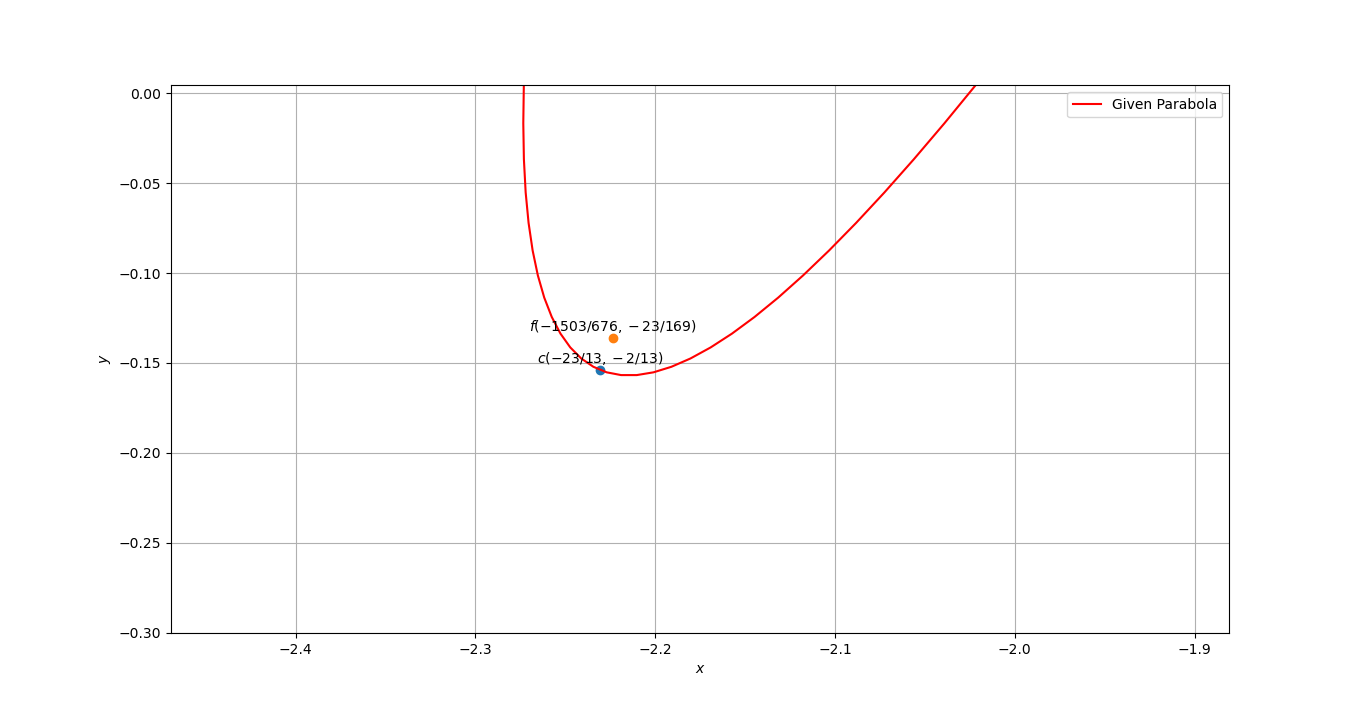
\includegraphics[angle=90,origin=c,width=\columnwidth]{./figs/parabola.eps}
\caption{}
\label{fig:parabola}
\end{figure}
%\begin{enumerate}[1.]
\numberwithin{equation}{enumi}
\item Show that the line 
\begin{align}
\myvec{4 & -2}\vec{x} + a= 0
\end{align}
touches the parabola 
\begin{align}
\vec{x}^T\myvec{0 & 0\\0 & 1}\vec{x}-4a\myvec{1 & 0 }\vec{x}= 0 
\end{align}
and find the coordinates of
the point of contact.
\item Find the point of intersection of the parabolas 
\begin{align}
\vec{x}^T\myvec{0 & 0\\0 & 1}\vec{x}-4a\myvec{1 & 0 }\vec{x}= 0 
\\
\vec{x}^T\myvec{1 & 0\\0 & 0}\vec{x}-4a\myvec{0 & 1 }\vec{x}= 0 
\end{align}
other than the origin, and prove that the tangents
at this point are inclined at an angle $\tan^{-1}\frac{3}{4}$.
\item Find the points in which the line 
\begin{align}
\myvec{8 & -1}\vec{x} = a
\end{align}
 cuts the parabola 
\begin{align}
\vec{x}^T\myvec{0 & 0\\0 & 1}\vec{x}-4a\myvec{1 & 0 }\vec{x}= 0 
\end{align}
and find the point where
the tangents at these points intersect.
\renewcommand{\theequation}{\theenumi}
\item A line through the vertex $\vec{A}$ of the parabola 
\begin{align}
\vec{x}^T\myvec{0 & 0\\0 & 1}\vec{x}-4a\myvec{1 & 0 }\vec{x}= 0 
\end{align}
makes an angle of $60\degree$ with
the axis and cuts the curve again in $\vec{P}$.  Find the equation of the tangent at $\vec{P}$,
and show that the area of the triangle this tangent makes with the axes is $\frac{4a^2}{3\sqrt{3}}$.
\item Prove that in  Fig. \ref{fig:parabola}
\begin{equation}
SG=SP
\end{equation}
\item Prove that $t_1t_2=-1$ is the condition that the chord joining the points with parameters $t_1, t_2$ on
a parabola shall pass through the focus.
\item Prove that the tangents drawn to a parabola from a point on the
directrix are at right angles and that their chord of contact passes
through the focus.
\item If in Fig. \ref{fig:parabola} $PS$ cuts the curve again in $\vec{Q}$, prove that $QA$ passes
through $\vec{M}$.
\item Through the vertex $\vec{A}$ of a parabola chords $AP$, $AP$ at right angles
to one another are drawn.  Prove that $PA$ cuts the axis in a fixed point.
\item Find the coordinates of the other point in which the normal at $\myvec{at^2\\2at}$
meets the parabola 
\begin{align}
\vec{x}^T\myvec{0 & 0\\0 & 1}\vec{x}-4a\myvec{1 & 0 }\vec{x}= 0 
\end{align}
;
 and prove that two normal chords that cut at right angles
divide one another in the ratio $1:3$.
\item Three normals are drawn to a parabola from the point $\myvec{h\\k}$.  Prove that
the centroid of the triangle formed by their feet is the point $\myvec{\frac{2}{3}\brak{h-2a}\\0}$.\numberwithin{equation}{enumi}
\item Find the equation of the tangent to the parabola 
\begin{align}
\vec{x}^T\myvec{0 & 0\\0 & 1}\vec{x}-4a\myvec{1 & 0 }\vec{x}= 0 
\end{align}
%
 that is parallel
to the normal at $\vec{P}= \myvec{at^2\\2at}$; and prove that, if this tangent meets the axis in $T$
and $PN$ is the ordinate of $P$ and $A$ is the vertex, then
\begin{equation}
TA.AN=a^2
\end{equation}
\item Prove that the circle 
\begin{align}
\vec{x}^T\vec{x}+2\myvec{g & f }\vec{x}+c= 0 
\end{align}
%
 cuts the parabola 
\begin{align}
\vec{x}^T\myvec{0 & 0\\0 & 1}\vec{x}-4a\myvec{1 & 0 }\vec{x}= 0 
\end{align}

 in four points the sum of
whose ordinates is zero; and conversely that if four ponits on a parabola be
such that the sum of their ordinates is zero then the four points lie on a circle.
\item Prove that the orthocentre of a triangle whose sides all touch a parabola
lies on the directrix.
\item A chord $POQ$ of a parabola 
\begin{align}
\vec{x}^T\myvec{0 & 0\\0 & 1}\vec{x}-4a\myvec{1 & 0 }\vec{x}= 0 
\end{align}

 cuts the axis in a fixed point $\vec{O}$.  $PN$, $QM$ are the ordinates of $\vec{P}$ and $\vec{Q}$,
and $\vec{A}$ is the vertex.  Prove that
\begin{align}
NP.MQ+4a.AO=0
\end{align}
\item From a point $\vec{P}= \myvec{at_1^2\\2at_1}$ on the parabola 
\begin{align}
\vec{x}^T\myvec{0 & 0\\0 & 1}\vec{x}-4a\myvec{1 & 0 }\vec{x}= 0 
\end{align}
 two chords $PQ$, $PR$ are drawn normal to the curve at $\vec{Q}$
and $\vec{R}$.  Prove that, if $\vec{Q}$, $\vec{R}$ are the points with parameters $t_2$, $t_3$ on the curve, then $t_2t_3=2$, and the equation
of $QR$ is
\begin{align}
\myvec{2 & t_1}\vec{x} + 4a= 0
\end{align}
\item Prove that the normals to a parabola at the ends of a chord whose inclination to the axis is $\theta$ meet on the
normal whose inclination is $\tan^{-1}\brak{2\cot\theta}$.
\item Prove that, if two parabolas are on the same side of the same directrix and have their axes in the same line, then they intersect
at a distance from the directrix equal to one-quarter of the sum of their latera recta.

\end{enumerate}
 
\subsection{Miscellaneous}
In the following problems, the equation of a parabola is assumed to be \eqref{eq:parab_standard}
and capital letters refer to Fig. \ref{fig:parabola} unless the contrary is stated.
\renewcommand{\theequation}{\theenumi}
\begin{enumerate}[label=\arabic*.,ref=\thesubsection.\theenumi]
\item Prove that as $\vec{P}$ moves along the curve $GP^2$ varies as $SG$.
\item Prove that, if $PP_1$ is a double ordinate and $PX$ meets the curve in $\vec{Q}$,
then $P_1Q$ passes through $\vec{S}$.
\item Prove that, if $PSP_1$ is a focal chord and $AP$, $AP_1$ meet the latus rectum in $\vec{Q}$, $\vec{Q}_1$,
the $SQ$, $SQ_1$ are equal to the ordinates of $\vec{P}_1$ and $\vec{P}$.
\item Prove that, if the tangents at $\vec{P}$, $\vec{Q}$ intersect in $\vec{T}$, then
\begin{align}
ST^2=SP.SQ.
\end{align}
\item Prove that, if the tangent at the end $\vec{Q}$ of a focal chord $PSQ$ meets the latus rectum
in $\vec{R}$, then $PGR$ is a right angle.
\item Tangents at $\vec{P}$, $\vec{Q}$, $\vec{R}$ on a parabola form a triangle $UVW$.  Show that the centroids of
the triangles $PQR$ and $UVW$ lie on the same diameter.
\item Prove that, if the difference of the ordinates of two points on a
parabola is constant, then the locus of the point of intersection of the tangents at
these points is an equal parabola.
\item Prove that, if two tangents intercept a fixed length on the tangent at the vertex, the locus
of their intersections is an equal parabola.
\item The chord of contact of tangents from any point $\vec{Q}$ meets the tangent
at the vertex in $\vec{R}$.  Prove that the tangent of the angle which $AQ$ makes with the axis
is $\frac{2a}{AR}$.
\item The parameters, $t$, $t_1$ of two points on a parabola are
connected by the relation $t=k^2t_1$, prove that the tangents at the points intersect on the
curve
\begin{align}
\vec{x}^T\myvec{0 & 0\\0 & 1}\vec{x}-\brak{k+\frac{1}{k}}^2a\myvec{1 & 0 }\vec{x}= 0 
\end{align}
\item Show that the length of the normal chord at the point of parameter $t$ is
\begin{align}
\frac{4a}{t^2}\brak{1+t^2}^{\frac{3}{2}}
\end{align}
\item Prove that the locus of intersection of tangents at the ends of a normal
chord is
\begin{align}
\brak{x+2a}y^2+4a^2=0.
\end{align}
\item Prove that the locus of the point of intersection of perpendicular normals
is the parabola 
\begin{align}
\vec{x}^T\myvec{0 & 0\\0 & 1}\vec{x}-a\myvec{1 & 0 }\vec{x}+ 3a^2 =0
\end{align}
\item Prove that if the tangents at two points on the parabola intersect in
the point $\myvec{x_1\\y_1}$, the corresponding normals intersect in the
point 
\begin{align}
\myvec{2a-x_1+\frac{y_1^2}{a}\\-\frac{x_1y_1}{a}}.
\end{align}
\item Show that, if the tangent at $\vec{P}$ meets the latus rectum in $\vec{K}$, then $SK$ is a mean
proportional between the segments of the focal chord through $\vec{P}$.
\item Show that, if the tangents from $\vec{Q}$ to the parabola form with the tangent at the vertex,
a triangle of constant area $c^2$, then the locus
of $\vec{Q}$ is the curve
\begin{align}
x^2\brak{y^2-4ax} = 4c^4.
\end{align}
\item Show that the normals at the ends of each of a series of parallel chords of a parabola intersect
on a fixed straight line, itself a normal to the parabola.
\item $\vec{P}$, $\vec{Q}$ are points on the parabola subtending a constant angle
$\alpha$ at the vertex.  Show that the locus of the intersection of the tangents
at $\vec{P}$, $\vec{Q}$ is the curve 
\begin{align}
\vec{x}^T\myvec{0 & 0\\0 & 1}\vec{x}-\myvec{4a + \frac{\tan^2\alpha}{4} & 0 }\vec{x}= a^2\tan^2\alpha 
\end{align}
\item Prove that the exterior angle between two tangents to a parabola is equal to the
angle which either of them subtends at the focus.
\item Two perpendicular focal chords of a parabola meet the directrix in $\vec{T}$ and $\vec{T}_1$.
Show that the tangents to the parabola which are parallel to these chords intersect in the middle point of $TT_1$.
\item Prove that, if the tangents at the points $\vec{Q}$, $\vec{R}$ intersect at $\vec{P}$, then 
\begin{align}
PQ^2:PR^2=SQ:SR
\end{align}
\item The tangents at any two points $\vec{P}$, $\vec{Q}$ meet at $\vec{T}$ and the normals meet at $\vec{N}$.  Prove that the projection
of $TN$ on the axis is equal to the sum of the distances of $\vec{P}$ and $\vec{Q}$ from the directrix.
\item Prove that the circumscribing circle of the triangle formed by three tangents to a parabola
passes through the focus.
\item $PQ$ is a chord of a parabola normal at $\vec{P}$; the circle on $PQ$ as diameter cuts the parabola again in $\vec{R}$.  Prove that the projection
of $QR$ on the axis is twice the latus rectum.
\item Prove that the distance between a tangent and the parallel normal is $a\text{cosec}\theta\sec^2\theta$, where $\theta$ is the
angle which either makes with the axis.
\item Prove that, if the normals at $\vec{P}$ and $\vec{Q}$ intersect on the curve, then $PQ$ cuts the axis in
a fixed point.
\item Prove that, if the normals at $\vec{P}$ and $\vec{Q}$ meet at the point $\vec{R}$ $\myvec{x_1,y_1}$ on the parabola, and the tangents at $\vec{P}$ and $\vec{Q}$
meet at $\vec{T}$, then
\begin{align}
TP.TQ=\frac{1}{2}\brak{x_1-8a}\sqrt{y_1^2+4a^2}.
\end{align}
\item Show that, in the last problem, as $\vec{R}$ moves along the parabola, the middle point of $PQ$
always lies on the parabola
\begin{align}
%\label{eq:parab_standard}
\vec{x}^T\myvec{0 & 0\\0 & 1}\vec{x}-2a\myvec{1 & 0 }\vec{x}= 4a^2 
\end{align}
\item Prove that the area of the triangle formed by the tangents at the points $t_1,t_2$, and their chord of 
contact is
\begin{align}
\frac{1}{2}a^2\brak{t_1-t_2}^2
\end{align}
\item Prove that the area of the triangle formed by three points $t_1$, $t_2$, $t_3$ on the parabola is
\begin{align}
a^2\brak{t_2-t_3}\brak{t_3-t_1}\brak{t_1-t_2}
\end{align}
and that this is double the area of the triangle formed by the tangents at these points.
\item Prove that, if a line through any point $P \myvec{x_1\\y_1}$ making an angle $\theta$ with the axis meets the parabola
at $\vec{Q}$ and $\vec{R}$, then
\begin{align}
PQ.PR = \brak{y_1^2-4ax_1}\text{cosec}^2\theta.
\end{align}
\item Two chords $QR$, $Q_1R_1$ of a parabola meet at $\vec{O}$, and the diameters bisecting them meet the curve at $\vec{P}$ and $P_1$.  Prove that
\begin{align}
QO.OR:Q_1O.OR_1=SP:SP_1
\end{align}
\item Show that, if $\vec{P}$ is on the parabola, the length of the chord through $\vec{P}$ that makes an angle $\theta$ with the axis is
\begin{align}
4a\sin\brak{\alpha-\theta}\text{cosec}^2\theta\text{cosec}\alpha
\end{align}
where $\alpha$ is the inclination of the tangent at $\vec{P}$ to the axis.
\item Show that the locus of the middle point of a chord which passes through the fixed point $\myvec{h\\k}$ is the parabola
\begin{align}
%\label{eq:parab_standard}
\vec{x}^T\myvec{0 & 0\\0 & 1}\vec{x}-\myvec{2a & k }\vec{x}+2ah= 0 
\end{align}
\item A tangent to the parabola 
\begin{align}
\vec{x}^T\myvec{0 & 0\\0 & 1}\vec{x}+4b\myvec{1 & 0 }\vec{x}= 0 
\end{align}
meets the parabola 
\begin{align}
\vec{x}^T\myvec{0 & 0\\0 & 1}\vec{x}-4a\myvec{1 & 0 }\vec{x}= 0 
\end{align}
at $\vec{P}$, $\vec{Q}$.  Prove that the locus of the middle point of $PQ$
is
\begin{align}
\vec{x}^T\myvec{0 & 0\\0 & 2a+b}\vec{x}-4a^2\myvec{1 & 0 }\vec{x}= 0 
\end{align}
\item Prove that the polar of the focus of a parabola is the directrix.
\item Prove that, if a chord of the parabola subtends a right angle at the vertex, the locus of its pole is 
\begin{align}
\myvec{1 & 0}\vec{x} + 4a= 0 
\end{align}
\item Show that, if parabolas 
\begin{align}
\vec{x}^T\myvec{0 & 0\\0 & 1}\vec{x}-4a\myvec{1 & 0 }\vec{x}= 0 
\end{align}
 are drawn corresponding to different values of $a$, the feet of the perpendiculars
from a fixed point on its polar lines all lie on a circle passing through the point.
\item Prove that, if from a point $\vec{Q}= \myvec{x_1\\y_1}$ a perpendicular be drawn to the polar
of $\vec{Q}$ with regard to the parabola cutting it in $\vec{R}$ and the axis in $G$, then
\begin{align}
SG=SR=x_1+a
\end{align}
\item Prove that, if the diameter through a point $\vec{P}$ of a parabola meets any chord in $\vec{O}$ and the tangents at the
ends of the chord in $\vec{T}, \vec{T}_1$, then
\begin{align}
PO^2=PT.PT_1
\end{align}
\item $QQ_1$ is a chord of a parabola and $TOR$ is a diameter which meets the tangent at $\vec{Q}$ in $\vec{T}$, the curve in $\vec{O}$ and $QQ_1$ in $\vec{R}$.  Prove
that 
\begin{align}
TO:OR=QR:RQ_1
\end{align}
\item Prove that if the normals at three points $\vec{P}$, $\vec{Q}$, $\vec{R}$ on a parabola concur, then the points $\vec{P}$, $\vec{Q}$, $\vec{R}$ and the vertex of
the parabola are concyclic.
\item Prove that in general, two members of the family of parabolas 
\begin{align}
\vec{x}^T\myvec{0 & 0\\0 & 1}\vec{x}-4a\myvec{1 & 0 }\vec{x}= 4a^2 
\end{align}
, where $a$ is the parameter specifying members
of the family, pass through any assigned point of the plane, and that these two parabolas cut orthogonally at $\vec{P}$.
\end{enumerate}
 
\section{The Ellipse}
\subsection{Properties}
\renewcommand{\theequation}{\theenumi}
\begin{enumerate}[label=\arabic*.,ref=\thesubsection.\theenumi]
\numberwithin{equation}{enumi}
\item Find the length of the latus rectum, the eccentricity and the coordinates of the
foci of the ellipses
\begin{enumerate}
\item 
$
\vec{x}^T\myvec{4 & 0\\0& 9}\vec{x} = 36
$
\item 
$
\vec{x}^T\myvec{9 & 0\\0& 4}\vec{x} = 36
$
\item
$
\vec{x}^T\myvec{1 & 0\\0& 2}\vec{x} = 8
$
\end{enumerate}
\item Find the equation of the ellipse whose foci are the points $\myvec{3\\0}$,  $\myvec{-3\\0}$
and eccentricity $\frac{1}{2}$.  What are the equations of the directrices?
\item Find the equation of the ellipse of eccentricity $\frac{3}{4}$, which has its centre at the point $\myvec{4\\0}$ and touches the axis of $y$ at the
origin.  What is the length of its latus rectum?
\item An ellipse has the axis of $y$ for directrix and its centre at the point $\myvec{6\\0}$.   Find its 
equation if its eccentricity is $\frac{3}{4}$.
\item Find the equation of the ellipse which has a focus at $\myvec{3\\1}$, corresponding directrix the line
\begin{align}
\myvec{1 & 0}\vec{x} = 6
\end{align}
and
eccentricity $\frac{1}{2}$.  What are the lengths of its axes?
\item An ellipse has its centre at $\myvec{2\\3}$ and a focus at $\myvec{3\\4}$ and its eccentricity is $\frac{1}{2}$.  Find its equation.
\item Are the points $\myvec{2\\1}$, $\myvec{3\\-2}$ inside or outside the ellipse
\begin{align}
\vec{x}^T\myvec{2 & 0\\0& 5}\vec{x} = 20
\end{align}
\item Prove that the line $y=x-5$ touches the ellipse
\begin{align}
\vec{x}^T\myvec{9 & 0\\0& 16}\vec{x} = 144
\end{align}
and find the coordinates of the point of contact.
\item The line 
\begin{align}
\myvec{2 & 3}\vec{x} = c
\end{align}
 touches the ellipse 
\begin{align}
\vec{x}^T\myvec{4 & 0\\0& 9}\vec{x} = 1
\end{align}
  Find the values of $c$.
\item Find the equation of the tangent to the ellipse 
\begin{align}
\vec{x}^T\myvec{1 & 0\\0& 4}\vec{x} = 8
\end{align}
 at the point $\myvec{2\\1}$, and also the equations of the two tangents perpendicular to this.
\item Find the equations of the tangents to the ellipse 
\begin{align}
\vec{x}^T\myvec{3 & 0\\0& 4}\vec{x} = 2
\end{align}
 which makes an angle of $60\degree$ with the major axis.
\item Find at what point the line 
\begin{align}
\myvec{e & 1}\vec{x} = a
\end{align}
touches the ellipse
\begin{align}
\vec{x}^T\myvec{1-e^2 & 0\\0& 1}\vec{x} = a^2\brak{1-e^2}
\end{align}
\item Prove that the normal at an end of the latus rectum meets the major axis at a distance $ae^3$ from the centre.
\item Prove that the normal at an end $L$ of the latus rectum meets the minor axis in $g$, and $l$ is the projection of $L$ on the
minor axis, then
\begin{align}
gl=a
\end{align}
\item Prove that the normal at $\myvec{x\\y}$ divides the major axis into segments of lengths $a-e^2x$ and $a+e^2x$.
\item Prove that if the normal at $\vec{P}$ meets the major axis in $\vec{G}$, and the minor axis in $\vec{G}_1$, then
\begin{enumerate}
\item $SG=eSP;$
\item $PG:PG_1 = b^2:a^2$
\end{enumerate}

\end{enumerate}
 
\subsection{Pole and Polar}
\renewcommand{\theequation}{\theenumi}
\begin{enumerate}[label=\arabic*.,ref=\thesubsection.\theenumi]
\numberwithin{equation}{enumi}
\item Find the polar of the point $\myvec{5\\7}$ with regard to the ellipse
\begin{align}
\vec{x}^T\myvec{2 & 0\\0 & 3}\vec{x} =6
\end{align}
\item Find the pole of the line 
\begin{align}
\myvec{3 & 4}\vec{x}=5
\end{align}
with regard to the ellipse
\begin{align}
\vec{x}^T\myvec{3 & 0\\0 & 4}\vec{x} =5
\end{align}
\item Find the poles of the lines 
\begin{align}
\myvec{2 & -1}\vec{x}=1
\\
\myvec{1 & 3}\vec{x}=4
\end{align}
with regard to the ellipse 
\begin{align}
\vec{x}^T\myvec{1 & 0\\0 & 4}\vec{x} =6,
\end{align}
 and verify that the line joining
the poles is the polar of the point of intersection of the lines.
\item Prove that the points $\myvec{4\\1}$, $\myvec{1\\-1}$ are conjugate with regard to the ellipse
\begin{align}
\vec{x}^T\myvec{2 & 0\\0 & 3}\vec{x} =5
\end{align}
\item Find the equatioin of a line through the point $\myvec{3\\2}$ and conjugate to the
line 
\begin{align}
\myvec{1 & 1}\vec{x}=1
\end{align}
with regard to the ellipse
\begin{align}
\vec{x}^T\myvec{3 & 0\\0 & 4}\vec{x} =2
\end{align}
\item Prove that, if the polar of a point is at right angles to the line joining the point  to
the centre of an ellipse, the point must lie on one of the axes.
\item Prove that, if $\myvec{x_2\\y_2}$ is the pole of the normal at $\myvec{x_1\\y_1}$, then
\begin{align}
\frac{x_1x_2}{a^4}=-\frac{y_1y_2}{b^4}  = \frac{1}{a^2-b^2}
\end{align}
\item Prove that a directrix of an ellipse is the polar of the corresponding focus.
\end{enumerate}
 
\subsection{Eccentric Angles}
\renewcommand{\theequation}{\theenumi}
The following problems refer to the ellipse whose 
equation is
\begin{align}
\vec{x}^T\myvec{b^2 & 0\\0 & a^2}\vec{x} =a^2b^2
\end{align}
\begin{enumerate}[label=\arabic*.,ref=\thesubsection.\theenumi]
\numberwithin{equation}{enumi}
\item Show that the eccentric angle of one end of a latus rectum is $\cos^{-1}e$.
\item If $\alpha$ is the eccentric angle of a point $\vec{P}$ on an ellipse, what are the coordinates of the
corresponding point $\vec{Q}$ on the auxilary circle?
Write down the equations of the tangents at $\vec{P}$ and $\vec{Q}$ and show that they intersect on the major axis.
\item Prove that, if $CP$, $CD$ are conjugate radii of an ellipse and $\omega$ the angle between them, then
$\sin^{2}\omega$ varies as $CP^{-2}+CD^{-2}$.
\item Prove that if a parallelogram is inscribed in an ellipse, its sides are parallel to 
the conjugate diameters.
\item Prove that if $QQ_1$ is a chord of an ellipse parallel to the tangent at $\vec{P}$ the eccentric angles
of $\vec{Q}$ and $\vec{Q}_1$ differ from the eccentric angle at $\vec{P}$ by equal amounts.
\item Prove that the equation of the perpendicular bisector of the chord joining the points $\vec{Q}$, $\vec{Q}_1$ whose
eccentric angles are $\alpha+\beta$, $\alpha-\beta$ is 
\begin{align}
\myvec{a\sec \alpha & -b\text{ cosec } \alpha}\vec{x} = \brak{a^2-b^2}\cos\beta
\end{align}
and deduce the equation of the normal at the point whose eccentric angle is $\alpha$.
\item Prove that, if the same chord passes through a focus, then
\begin{align}
\cos\beta = \pm e \cos\alpha
\end{align}
\item Prove that the equation of a focal chord parallel to the tangent at the point whose
eccentric angle is $\alpha$ is
\begin{align}
\myvec{\frac{\cos\alpha}{a}  & \frac{\sin\alpha}{b}}\vec{x} = \pm e \cos\alpha
\end{align}
\item Prove that, if $\alpha$ is variable and $\beta$ constant, the chord joining the points whose eccentric angles are $\alpha+\beta$
and $\alpha-\beta$ touches the
ellipse
\begin{align}
\vec{x}^T\myvec{b^2 & 0\\0 & a^2}\vec{x} =a^2b^2\cos^2\beta
\end{align}
and that the locus of the poles of the chord is
\begin{align}
\vec{x}^T\myvec{b^2 & 0\\0 & a^2}\vec{x} =a^2b^2\sec^2\beta
\end{align}
\item Prove that the tangents at the points whose eccentric angles are $\alpha$, $\alpha+\frac{\pi}{2}$ intersect on the ellipse
\begin{align}
\vec{x}^T\myvec{b^2 & 0\\0 & a^2}\vec{x} =2a^2b^2
\end{align}
\item Prove that, if $\vec{P}$, $\vec{Q}$ are corresponding points on an ellipse and its auxiliary circle and the normals
at $\vec{P}$, $\vec{Q}$ intersect in $R$, then
\begin{align}
CR = a+b
\end{align}
\item Prove that, if the line joining the ends of two equal conjugate radii of an ellipse passes through
a focus the eccentricity is $\frac{1}{\sqrt{2}}$.
\item Prove that the chords that join the ends of conjugate radii all touch the ellipse
\begin{align}
2\vec{x}^T\myvec{b^2 & 0\\0 & a^2}\vec{x} =a^2b^2
\end{align}

\end{enumerate}
 
\subsection{Miscellaneous}
\renewcommand{\theequation}{\theenumi}
\begin{enumerate}[label=\arabic*.,ref=\thesubsection.\theenumi]
\numberwithin{equation}{enumi}
\item The following problems refer to the ellipse whose 
equation is
\begin{align}
\vec{x}^T\myvec{b^2 & 0\\0 & a^2}\vec{x} =a^2b^2
\end{align}
and that $C$ is its centre and $S$, $S_1$ its foci.

\item Prove that, if the tangent and normal at a point $P$ on an ellipse meet the major axis
in $T$, $G$, then the tangent from either end of the minor axis to the circle $TPG$ is equal in length to half the major
axis.
\item Show that if $\myvec{x_1\\y_1}$ are the coordinates of a point of intersection of the ellipses
\begin{align}
\vec{x}^T\myvec{b^2 & 0\\0 & a^2}\vec{x} =a^2b^2
\end{align}
 and 
\begin{align}
\vec{x}^T\myvec{b_1^2 & 0\\0 & a_1^2}\vec{x} =a_1^2b_1^2
\end{align}
the equations of their common tangents are 
\begin{align}
\myvec{\pm \dfrac{x_1}{aa_1} & \pm \dfrac{y_1}{bb_1}}\vec{x} = 1
\end{align}
\item The normal at any point $P$ of the ellipse meets the axis in $G$; a point $Q$ is taken in the
tangent so that $PQ=\lambda.PG$, where $\lambda$ is constant; prove that the locus of $Q$ is the ellipse
\begin{align}
\vec{x}^T\myvec{b^2 & 0\\0 & a^2}\vec{x} =a^2b^2\frac{a^2+\lambda b^2}{a^2}
\end{align}
\item Prove that the line 
\begin{align}
\myvec{\dfrac{a}{k^2-1} & \dfrac{b}{2k}}\vec{x} +\dfrac{a^2-b^2}{k^2+1} = 0
\end{align}
 is a normal to the ellipse 
\begin{align}
\vec{x}^T\myvec{b^2 & 0\\0 & a^2}\vec{x} =a^2b^2
\end{align}
for all values of $k$.
\item Prove that the foot of the focal perpendicular on the normal at any point of an ellipse is at
a distance from the centre equal to the difference between the semi-major axis and the focal
radius vector to the point at which the normal is drawn.
\item Prove that the locus of the poles of normal chords of the ellipse is the curve
\begin{align}
\frac{a^6}{x^2}+\frac{b^6}{y^2}=\brak{a^2-b^2}^2.
\end{align}
\item $P$ is a point $\myvec{x_1\\y_1}$ on the ellipse and $PS$, $PS_1$ meet the curve again in $Q$, $R$.  Prove that
the equation of $QR$ is 
\begin{align}
\myvec{\frac{x_1}{a^2} &\frac{y_1}{b^2}\frac{1+e^2}{1-e^2}}\vec{x} + 1 = 0,
\end{align}
where $e$ is the eccentricity.
\item Show that two parallel tangents to an ellipse are met by any other tangent in points
which lie on conjugate diameters.
\item Prove that if $CP$, $CD$ be any two conjugate semi-diameters of an ellipse and $PF$ be drawn
perpendicular to $CD$ and produced both ways to $E$, $E_1$ so that
$PE=PE_1=CD$, then $CE.CE_1=CS^2$, where $S$ is a focus.
\item Tangents are drawn from points on the ellipse to the circle 
\begin{align}
\norm{\vec{x}} = r
\end{align}
, show that the chords of contact touch
the ellipse
\begin{align}
\vec{x}^T\myvec{a^2 & 0\\0 & b^2}\vec{x} =r^4
\end{align}
\item Tangents $TP$, $TQ_1$ are drawn to an ellipse so that $SP$, $S_1Q$ are parallel.  Prove that $CT$ is parallel to $SP$ or $S_1Q$.
\item the normal to an ellipse at a point $P$ passes through one end of the minor axis, and $CD$ is the semidiameter conjugate to $CP$.  The
perpendicular from $C$ to $CD$ meets the auxiliary circle in $E$.  Prove that $DE$ is equal to half the distance
betwen the directrices.
\item Prove that, if $\myvec{x_1\\y_1}$ be the middle point of a chord of the ellipse, the equation of the chord is
\begin{align}
\myvec{\frac{x_1}{a^2} &\frac{y_1}{b^2}}\vec{x} = \frac{x_1^2}{a^2}+\frac{y_1^2}{b^2}
\end{align}
\item  If $Q$ be the pole of the chord of the ellipse which is normal at a point $P$, and if
$CR$ drawn through the centre $C$ perpendicular to $CQ$ meet the normal at $P$ in $R$, prove that the locus of $R$ is
\begin{align}
\vec{x}^T\myvec{a^6 & 0\\0 & b^6}\vec{x} =a^4b^4
\end{align}
\item Prove that, if the point $P$ lies on the ellipse 
\begin{align}
\vec{x}^T\myvec{b_1^2 & 0\\0 & a_1^2}\vec{x} =a_1^2b_1^2
\end{align}
 its polar with regard to the 
ellipse 
\begin{align}
\vec{x}^T\myvec{b^2 & 0\\0 & a^6}\vec{x} =a^2b^2
\end{align}
touches
the ellipse
\begin{align}
\vec{x}^T\myvec{a_1^2b^4 & 0\\0 & b_1^2a^4}\vec{x} =a^4b^4
\end{align}
\item Show that the polar with regard to the ellipse 
\begin{align}
\vec{x}^T\myvec{b^2 & 0\\0 & a^6}\vec{x} =a^2b^2
\end{align}
of a point on the circle 
\begin{align}
\norm{\vec{x}} = c
\end{align}
 touches the ellipse 
\begin{align}
\vec{x}^T\myvec{b^4 & 0\\0 & a^4}\vec{x} =\frac{a^4b^4}{c^2}
\end{align}
\item Prove that, if the tangents to an ellipse at $\myvec{x_1\\y_1}$ and $\myvec{x_2\\y_2}$ meet at $\myvec{x\\y}$ and the normals at
$\myvec{\xi\\\eta}$, then $a^2\xi=e^2xx_1x_2$ and $b^2\eta = -e^2yy_1y_2$, where $e$ is the eccentricity.
\item Show that, if $\myvec{x\\y}$ is the middle point of a chord of the ellipse,
and the tangents at the ends of the chord intersect in $\myvec{x_1\\y_1}$ and the normals
in $\myvec{x_2\\y_2}$, then
\begin{align}
\frac{a^2x_2}{x_1}+\frac{b^2y_2}{y_1}=\brak{a^2-b^2}\brak{\frac{xx_1}{a^2}-\frac{yy_1}{b^2}}.
\end{align}
\item Prove that, if the normals at two points $P$, $Q$ on an ellipse intersect on the diameter
that bisects $PQ$, then the two normals are at right angles.
\item Prove that if a chord of the ellipse subtends a right angle at the centre
then it touches the circle
\begin{align}
\norm{\vec{x}} = \frac{ab}{\sqrt{a^2+b^2}}
\end{align}
\item The locus of middle points of chords of the ellipse which subtend a right angle at its centre is
\begin{align}
\frac{x^2}{a^4}+\frac{y^2}{b^4}=\frac{a^2+b^2}{a^2b^2}\brak{\frac{x^2}{a^2}+\frac{y^2}{b^2}}^2
\end{align}
\item Show that the tangents at the extremities of all chords of the
ellipse which subtend a right angle at the centre, intersect on the ellipse
\begin{align}
\vec{x}^T\myvec{b^4 & 0\\0 & a^4}\vec{x} =a^2b^2\brak{a^2+b^2}
\end{align}
\item If $P$ be any point on the ellipse whose axes are $AA_1$, $BB_1$ and if the parallel lines
$AP$, $BQ$ be drawn, $Q$ being on the ellipse; $Q$ will be one
extremity of the diamter conjugate to that drawn from $P$.
\item From a any point $T$ on one of the equiconjugate diamters of a conic whose centre is $O$, tangents $TP$, $TQ$ are drawn to 
the conic.  Show that $O$, $P$, $Q$, $T$ are concyclic.
\item Prove that, if two conjugate radii of an ellipse cut the
director circle in $T$, $T_1$ then $TT_1$ touches the ellipse.
\item If $PSP_1$, $QSQ_1$ be two focal chords and if $PQ$ be parallel to the major axis, show that $P_1Q_1$ bisects the distance
between $S$ and the nearer directrix.
\item Tangents are drawn at the extremities of conjugate diameters of an ellipse, and meet in $O$.  Prove that the
perpendicular from $O$ on the focal radius to a point of contact is half the
minor axis.
\item Show that the area of the rectangle fromed by two parallel tangents and the corresponding
normals to an ellipse is never greater than half the square on the line joining the foci.
\item Prove that the angle btween the normal and the central radius at a point on an ellipse
is greatest when the point is the end of one of the equiconjugate diameters.
\item $P$, $Q$ are two points on the ellipse, and $PS$, $QS_1$ intersect on the curve, prove that the locus of the pole of $PQ$ is
\begin{align}
\vec{x}^T\myvec{\brak{2a^2-b^2}^2 & 0\\0 & a^2b^2}\vec{x} =a^2\brak{2a^2-b^2}^2
\end{align}
\item Two conjugate diameters of an ellipse meet a fixed straight line 
\begin{align}
\myvec{l & m}\vec{x} = 1
\end{align}
 in $P$, $Q$, and the straight lines
through $P$, $Q$ perpendicular to these diameters intersect in $R$;  prove that the locus of
$R$ is the straight line
\begin{align}
\myvec{a^2l & b^2m}\vec{x} = a^2+b^2
\end{align}
\item Prove that if $\alpha$, $\beta$ are the eccentric angles of two points $P$, $P_1$ on an ellipse such that
the focal distances $SP$, $S_1P_1$ are parallel, then 
\begin{align}
\tan\frac{\alpha}{2}:\tan\frac{\beta}{2} = 1\pm e: 1\mp e,
\end{align}
and $PP_1$ touches the ellipse
\begin{align}
\vec{x}^T\myvec{b^4 & 0\\0 & a^4}\vec{x} =a^2b^4
\end{align}
\item Prove that the square of the sum of two conjugate radii is greatest when the radii are equal.
\item Prove that, if on the inward normal to an ellipse at $P$ a length $PQ$ be taken
equal to the conjugate radius $CD$, the locus of $Q$ is a circle of radius $a-b$.
\item Prove that, if $P$, $Q$ are corresponding points on an ellipse and its auxiliary circle, and the
normal at $P$ to the ellipse meets the normal at $Q$ to the circle in $R$, then the locus of $R$ is a circle of radius $a+b$.
\item Prove that, if lines drawn from any poin on an ellipse to the ends of a diameter $PCP_1$ meet the conjugate
diameter $DCD_1$ in $M$, $M_1$, then $CM.CM_1=CD^2$.
\item Prove that, if an ellipse slides between two straight lines
at right angles to one another, the locus of its centre is a circle.
\end{enumerate}
 
\subsection{Hyperbola}
\renewcommand{\theequation}{\theenumi}
\begin{enumerate}[label=\arabic*.,ref=\thesubsection.\theenumi]
\numberwithin{equation}{enumi}
\item Show that the eccentricity of a rectangular hyperbola is $\sqrt{2}$
\item Prove that the locus of the centre of a circle which touches two
given non-concentric circles of unequal radii is an ellipse or a hyperbola.
\item $ABC$ is a triangle in which $C$ is a right angle.  On $CA$, $CB$ points $P, Q$ are
taken such that $CP.CQ=CA.CB$.  Prove that the locus of the centroid of the trianlge $CPQ$ is a rectangular hyperbola.
\item Show that the tangents to a rectangular hyperbola at the extremities of its latera
recta pass through the vertices of the conjugate hyperbola.
\item $P$ is a point on a rectangular hyperbola whose centre is $C$ and a 
line is drawn through $C$ perpendicular to $CP$.  Through
$Q$, any point on the curve, lines are drawn parallel to the asymptotes meeting
this line in $L$, $M$, show that $LPM$ is a right angle.
\item Prove that the intercept on any tangent to a hyperbola, made by its asymptotes, subtends a constant
angle at either focus.
\item Prove that the line $lx+my=n$ touches the rectangular hyperbola $xy=c^2$, if
\begin{align*}
n^2 = 4lmc^2
\end{align*}
\item A tangent to a hyperbola of foci $S$, $S_1$ meets the asymptotes
in $L$, $L_1$.  Prove that the points $S, L, S_1, L_1$ are concyclic.
\item The tangents at two points $P$, $P_1$ on a rectangular hyperbola meet an asymptote in $L, L_1$ and
$P,P_1$ meets it in $K$.  Prove that
\begin{align*}
LK = KL_1
\end{align*}
\item Prove that conjugate diameters of a rectangular hyperbola are equally inclined to the asymptotes.
\item Prove that the polars of a point with regard to two conjugate hyperbolas are parallel and equidistant from the
centre.
\item Prove that in a rectangular hyperbola any chord $PP_1$ subtends at the ends of a diameter $AA_1$ 
angles which are either equal or suplementary.
\item Prove that if $CP$, $CD$ are conjugate radii of a hyperbola the orthocentre of
the triangle $CPD$ lies on the line $ax=by$.
\item Prove that, if the tangent at $P$ to a rectanglular hyperbola meets the asymptotes in $L$, $L_1$ and
the normal at $P$ meets the transverse axis in $G$, then $LGL_1$ is a right angle.
\item Prove that if an ellipse and a hyperbola have the same foci they cut one another at right
angles.
\item The perpendiculars from a point $P$ to the axes meet them in $M, N$, and the perpendicular bisector
of $MN$ passes through a fixed point $C$ on one of the axes.  Prove that the locus of $P$ is a rectangular
hyperbola with centre at $C$.
\item Show that the locus of the middle point of a chord of the rectangular 
hyperbola $xy=c^2$ of constant length $2a$ is
\begin{align*}
\brak{xy-c^2}\brak{x^2+y^2} = a^2xy
\end{align*}
\item Prove that, if the position of a point on  a rectangular hyperbola is determined by the
variable $\theta$ where $x = c \tan\theta$, $y = c\cot\theta$, the locus of the intersection of tangents at the 
points $\theta$, $\theta+\alpha$ is
\begin{align*}
4\brak{c^2-xy} = \brak{x+y}^2\tan^2\alpha
\end{align*}
$\alpha$ being a constant angle.
\item Tangents at right angles are drawn to a rectangular hyperbola and its
conjugate.  Show that they cut either asymptote in two points
$K$, $K_1$ such that the rectangle $CK.CK_1$ is equal to twice the square on
the semi-axis, where $C$ is the centre.
\item Prove that the line joining the feet of the perpendiculars drawn to a
pair of conjugate diameters of a rectangular hyperbola from any point $P$ on the
hyperbola is parallel to the normal at $P$.
\item  The normal at $P_1$ on the hyperbola $xy-c^2=0$ meets the curve again at $P_2$, the normal at $P_2$
 meets the curve again at $P_3$
and so on.  Prove that if $y_1,y_2,\dots, y_{n+1}$ are the ordinates of these points respectively,
\begin{align*}
y_1^2y_2 = y_2^2y_3 = \dots = y_n^2y_{n+1} = c^4.
\end{align*}
\item If $PN$ be the ordinate and $PG$ the normal of a point $P$ of a hyperbola, whose centre is $C$, and the tangent
at $P$ intersect the asymptotes at $L$ and $L_1$, show that half the sum of $CL$ and $CL_1$ is the mean
proportional between $CN$ and $CG$.
\item At the point of intersection of the rectangular hyperbola $xy=k^2$, and of the parabola $y^2=4ax$, the tangents
to the hyperbola and parabola make angles $\theta$ and $\phi$ respectively with the axis of $x$.  Prove that
\begin{align*}
\tan\theta = -2\tan\phi.
\end{align*}
\item Prove that, if $A, B, C$ are three points on a rectangular hyperbola, the curve passes through the orthocentre
of the triangle $ABC$.
\item Prove that, in a rectangular hyperbola, the product of the focal distances of a point is equal
to the square of the distance of the point from the centre.
\item Prove that, if $\brak{c\tan\theta,c\cot\theta}$ and $\brak{c\tan\theta_1,c\cot\theta_1}$ are two points on 
the hyperbola $xy=c^2$, and $\theta+\theta_1$ is constant, then the chord
joining the points passes through a fixed point on the conjugate axis of the hyperbola.
\item Show that the point whose coordinates are
\begin{align*}
\frac{a}{2}\brak{t+\frac{1}{t}}, \frac{b}{2}\brak{t-\frac{1}{t}}
\end{align*}
lies on the hyperbola $\frac{x^2}{a}-\frac{y^2}{b^2} = 1$. Prove that, if $C$ is the centre of the hyperbola and $S$ is either focus 
and if the tangent at the above point meets the asymptote $\frac{x}{a}=\frac{y}{b}$ at $X$ and meets the asymptote $\frac{x}{a}=-\frac{y}{b}$
 at $Y$, then
\begin{align*}
t = \frac{CX}{CS} = \frac{CS}{CY}
\end{align*}
\item From any point on the normal at a given point $A$ on a rectangular hyperbola the other three normals to
the curve are drawn.  Sow that the centroid of the feet of these three normals lies on the diameter of the hyperbola
parallel to the normal at $A$.
\item A circle is drawn passing through any point $P$ on the hyperbola $\frac{x^2}{a^2}-\frac{y^2}{b^2}=1$ and through the ends $A$, $A_1$ of
the transverse axis.  The ordinate $NP$ is produced to  meet the circle again in $Q$.  Prove that, as
the position of $P$ on the hyperbola varies, the locus of $Q$ is the hyperbola $\frac{x^2}{a^2}-\frac{y^2}{b_1^2} = 1$, where $b_1 = \frac{a^2}{b}$.
\end{enumerate}
 
\section{Polar Coordinates}
\renewcommand{\theequation}{\theenumi}
\begin{enumerate}[label=\arabic*.,ref=\thesubsection.\theenumi]
\numberwithin{equation}{enumi}
\item Find the polar equations of the curves whose cartesian equations are:
\begin{enumerate}
\item 
$
x^2+y^2+2gx+2hy+c = 0
$
\item 
$
x^2+y^2 = ax
$
\item 
$
x^2-y^2=c^2
$
\item 
$
xy = \frac{c^2}{2}
$
\item 
$
x^3-8xy^2 = a^3.
$

\end{enumerate}
\item Find the Cartesian equations corresponding to the following
equations in polar coordinates:
\begin{enumerate}
\item 
$
r\sin\theta + a = 0
$
\item 
$
r = a\sin\theta + b\cos\theta
$
\item 
$
r^2\cos2\theta = a^2
$
\item 
$
\frac{1}{r} = 1 + e\cos\theta
$
\item 
$
r^3\sin3\theta = a^3
$
\item 
$
r^2=a^2+b^2\cos2\theta
$
\end{enumerate}
\item Using the polar equation of a conic with focus as pole, show that
the semi-latus rectum is a harmonic mean between the segments of
a focal chord.
\item Draw the curve $r=a\cos2\theta$, noting carefully when $r$
changes sign and showing that the curve forms a double figure of eight.
\item Draw the curve
\begin{align*}
r = a\brak{2+\cos\theta}
\end{align*}
\item Draw the curve $r = a\brak{1+2\cos\theta}$, showing that it consists of two loops one within
the other.
\item Deduce from the polar equations of the curves the pedal equations for
the circle, parabola with focus as pole, ellipse with focus as pole and
ellipse with centre as pole.
\item Find the pedal equation of:
\begin{enumerate}
\item The rectangular hyperbola
$
xy = c^2
$
\item the lemniscate 
$
r^2=a^2\cos2\theta
$
\item the curve 
$
r^n = a^n\cos n\theta
$
\item the spiral
$
r\theta = a.
$
\end{enumerate}
\item Prove that, for the curve $r\theta = a$, if a perpendicular through the pole be drawn
to the radius vector at any point, the length intercepted on it by the tangent
is constant.  
\item Prove that, for the curve $r = a \cos\brak{\theta-\alpha}$, $\phi = \frac{\pi}{2}+\theta-\alpha$.
\item Show that, for the curve $r = a\brak{1+\cos\theta}$, the locus of the foot of the perpendicular from the pole to the tangent is 
$r = 2a\cos^3\frac{\theta}{3}$.
\item Prove that, for the curve $r = a\sec^3\frac{\theta}{3}$, the locus of the foot of the perpendicular from the pole to the tangent
is a parabola.
\item Trace the curve $r^2=a^2\cos\theta$.
\item Prove that the pedal equation of the curve $r\cos n\theta = a$ is
\begin{align*}
\frac{1}{p^2} = \frac{1-n^2}{r^2}+\frac{n^2}{a^2}
\end{align*}
\end{enumerate}
 
\section{Easy Problems}
\subsection{The Straight Line}
\renewcommand{\theequation}{\theenumi}
\begin{enumerate}[label=\arabic*.,ref=\thesubsection.\theenumi]
\numberwithin{equation}{enumi}
\item Find the distance between the pionts $A$, $B$ whose coordinates are $\brak{3,7}$ and $\brak{11,13}$.  Also
find the coordinates of the point which divides $AB$ in the ratio $3:1$.
\item Find the equations of the sides of a triangle whose corners are at the points
$\brak{3,4}$, $\brak{-3,2}$, $\brak{2,-4}$.
\item In the last problem, find the equations of the perpendiculars from the corners of the triangle
to the opposite sides and verify that they meet in a point.
\item Find the distance between the points $A \brak{2,3}$ and $B \brak{14,8}$.  Find also the equation of the line $AB$ and
the distance from it of the point $C \brak{5,6}$.  What is the area of the triangle $ABC$?
\item The equations of the sides of a triangle are $x+y=5$, $2x-y+4=0$ and $x-4y+4=0$.  Find the tangents of the angles of
the triangle.
\item Find the equation of a line parallel to the line $5x+4y=9$ and making an intercept $-5$ 
on the $x$-axis.
\item Find the equations of two straight lines which pass through the intersection
of the lines $3x+4y=7$, $5x-2y=3$ and are parallel and perpendicular respectively to the line $2x+7y=3$.
\item Find the value of $k$ if the three lines $2x+5y=12$, $7x+2y=11$ and $kx-3y=10$ meet in a point.
\item Prove that the points $\brak{x_1,y_1}$, $\brak{x_2,y_2}$ and
\begin{align*}
\brak{\frac{x_1+kx_2}{1+k},\frac{y_1+ky_2}{1+k}}
\end{align*}
are collinear.
\item Show that the points $\brak{2,3}$ and $\brak{-1,2}$ are on opposite sides of the line $2x-3y=7$.  What are their distances from the line?
\item Two straight lines $AB$, $CD$ bisect one another at right angles.  The coordinates of $A$, $B$ and $C$ are
$\brak{1,5}$, $\brak{3,1}$ and $\brak{-1,1\frac{1}{2}}$.  Find the coordinates of $D$ and the area $ABCD$.
\item Prove that the line $2x+3y=5$ divides the join of the points $\brak{3,-5}$, $\brak{2,1}$ in the ratio $7:1$.
\item Find the equations of the two straight lines which pass through the point $\brak{3,2}$ and make angles of $45\degree$ with the line $4x-5y=6$.
\item Find the equation of the perpendicular bisector of the join of the points $\brak{3,5}$, $\brak{-6,7}$.
\item From a point $A \brak{2,5}$ a perpendicular $AB$ is drawn to the line $3x-4y=8$.  $AB$ is then produced to $C$ so that $BC=3AB$.  Find
the coordinates of $C$.
\item The sides $BC$, $CA$, $AB$ of a triangle have equations $3x+4y=9$, $4x-3y+6=0$, $5x-12y+12=0$.  Find the equations of the
bisectors of the interior angles of the triangle and the coordinates of their point
of concurrence.
\item $ABC$ and $DBC$ are two triangles such that $DB=AB$ and $DC=AC$.  The coordinates of $A$, $B$, $C$
are $\brak{3,1}$, $\brak{2,2}$, $\brak{-1,3}$.  Find the coordinates of $D$.  Also find the equations of $AD$ and $BC$ and verify that these lines are at right angles.
\item Find the centre of the inscribed circle of the triangle formed by the lines $3x-4y+8=0$, $4x+3y-9=0$, $y=6$.
\item Find the equations of two lines passing through the intersection of the lines $x+3y=5$ and $4x-y+2=0$,
and perpendicular and parallel respectively to the line $5x-3y+3=0$.
\item Find the equation of the line which passes through the intersection of the lines $2x+3y=4$ and $3x-y+2=0$
and also through the intersection of the lines $x+y=0$, $4x-y+3=0$.
\item Prove that the points $A \brak{4,2}$ and $C \brak{-3,1}$ subtend a right angle at $B \brak{-\frac{17}{13}, -\frac{20}{13}}$.  Find the coordinates of $D$, the remaining
corner of the rectangle $ABCD$, and verify that $DB=AC$.
\item The points $A \brak{4,2}$, $B \brak{1,-2}$, $C \brak{-3,1}$ and $D$ are the corners of a parallelogram.
Find the coordinates of $D$ and prove that the parallelogram is equal in area to the square on $OD$
where $O$ is the origin.
\item Show that the equation $6x^2+7xy-3y^2+x+7y-2=0$ represents two straight lines, and find the tangents of the angles between then.
\item Find the separate equations of the two straight lines represented by the
equation $x^2-2xy\cosec\theta + y^2 = 0$.  Also find the angles between the lines, and show that these angles are bisected by the lines
$x^2-y^2 = 0$.
\end{enumerate}
 
\subsection{Curves and Loci}
\renewcommand{\theequation}{\theenumi}
\begin{enumerate}[label=\arabic*.,ref=\thesubsection.\theenumi]
\numberwithin{equation}{enumi}
\item Find the equations of the tangents to the curves $y=x^3-x$ and $x^2-3x+2$ at their point of intersection, and the angle at which the
curves cut.
\item Prove that the line $3y=9x-16$ is a tangent to the curve $3y=x^3-3x$, and find the coordinates of the 
point of contact.
\item Prove that the tangents to the curve $y=x^3-6x^2+13x-6$ at the points $\brak{1,2}$ and $\brak{3,6}$ are parallel, and that
the tangent at the point $\brak{2,4}$ is inclined to them at an angle $\tan^{-1}\frac{3}{5}$.
\item Prove that the line $y=5x$ is a tangent to the curve
\begin{align*}
y=x^3-2x^2+x+8
\end{align*}
and find the coordinates of the point of contact.  In what other point does the line $y=5x$ meet the curve?
\item Find the equation of the tangent to the curve $y=3x^2-2x-1$ at the point $\brak{2,7}$.  Also find the coordinates of the point on the curve the tangent
at which is perpendicular to the tangent at $\brak{2,7}$.
\item Find the equation of the normal to the curve $y=2x^2-3x-5$ at the point $\brak{2,-3}$ , and find the length of the subnormal at this point.
\item Find the equation of the tangent to the curve
\begin{align*}
3y=x^3-6x^2-12x+1
\end{align*}
at the point $\brak{-1,2}$, and find the coordinates of another poin on the curve where the tangent
is parallel to that at $\brak{-1,2}$.
\item Prove that at every point of the curve $y=x^3-3x^2+3x+7$ the gradient is positive.  Table the values of $y$ and $\frac{dy}{dx}$ at the points
$x=-1,0,1,2,3$ and make a rought drawing of the curve.
\item Find the equation of the tangent and normal to the curve $y=\brak{x-1}^4$ at the point $\brak{2,1}$.  Find the area of the triangle
which the tangent and normal make with the $x$-axis.
\item Show that the curve $y=1-2x+x^3$ cuts the $x$-axis in three real points.  Find the gradient of the curve
at the point $\brak{1,0}$; also find the points at which the gradient vanishes and make a rough drawing of 
the curve.
\item Find the gradients of the curve $y=\brak{x-1}^2\brak{x-2}$ at the points where it crosses the axes.  Find also the points
at which the gradient vanishes and make a rough drawing of the curve.
\item Find the points on the curve $y=x^3-x^2+1$ at which the gradient is unity.  Find the equations of the tangents
and normals at these points.
\item Find the points in which the curve $y=1+2x-3x^2$ cuts the coordinate axes and find the gradients of the curve
at these points.  At what point does the gradient vanish?  Make a rough drawing of the
curve.
\item Show that the curve $y=\brak{x^2-1}^2$ is symmetrical about the $y$-axis.  Find its gradient and the points at which
the gradient vanishes.  In what points does the line $y=9$ cut the curve?  Make a rough drawing of the curve.
\item Show that the curve $y=x^4-4x^2$ is symmetrical about the $y$-axis.  Find the gradients of the curve
at its intersections with the $x$-axis.  find also the points where the gradient vanishes and make a
rough drawing of the curve.

\item Show that the curve $y=x^4-4x^2$ is symmetrical about the $y$-axis.  Find the gradients of the curve at its intersections
with the $x$-axis.  Find also the points where the gradient vanishes and make a rough drawing of the curve.
\item Find the gradient of the curve $y=x^2-3x-4$, and the point on the curve at which the gradient vanishes.  Also find
the gradient at the points where the curve crosses the $x$-axis and make a rough drawing of the curve.  To what
point on the $x$-axis must the origin be moved so that the curve may become symmetrical
about the $y$-axis, and what will be the equation of the curve when the position of the origin
is so changed?
\item Show that the curve whose equation is $27y=x^3-27x$ is symmetrical in opposite quadrants.  Prove that
the tangent to the curve at the origin is $x+y=0$.  Find the gradient at the other intersections with the $x$-axis.  Also
find at what points the tangent is parallel to the $x$-axis, and make a rough drawing of the curve.
\item Find the equation of the locus of a point which moves so that its distance from the point $\brak{2,1}$
is twice its distance from the line $3x+4y=2$.
\item Find the locus of a point which moves so that its distance from the origin is half the  distance from the
line $3x+4y=2$.
\item A point $P$ moves so that $PA^2+PB^2=AB^2$, where $A$, $B$ are the points $\brak{2,0}$, $\brak{0,3}$.  Find the equation of the locus of $P$.
\item Find the locus of a point whose distance from the point $A\brak{3,0}$ is three times its distance from the point $B \brak{-1,0}$.
Prove that the tangents to the locus at the points $\brak{0,0}$ and $\brak{-3,0}$ are parallel to the $y$-axis.
\item The coordiantes of a point are given in terms of a variable parameter $t$ by the relations $x=\frac{t}{t+1}, y = \frac{t}{t-1}$.  Find the equation of the locus
of the point, and prove that the equation of the tangent at any point $t$
on the locus is $\brak{t+1}^2x+\brak{t-1}^2y=2t^2$.
\item The coordinates of a point are given by the relations $x = t + \frac{1}{t}$, $y = t - \frac{1}{t}$ and $t$ is a variable parameter.  Find the
equation of the locus of the point for different values of $t$, and also the equations of the
tangent at the point denoted by $t$.
\end{enumerate}
 
\subsection{The Circle}
\renewcommand{\theequation}{\theenumi}
\begin{enumerate}[label=\arabic*.,ref=\thesubsection.\theenumi]
\numberwithin{equation}{enumi}
\item Prove that the circle of centre $\brak{3,4}$ and rdius 5 passes
through the origin.  Find the equations of the tangent at the origin 
and of the parallel tangent.  IN what other points does the circle
cut the axes?
\item find the equation of a circle having the points $\brak{2,1}$
and $\brak{1,-3}$ for the ends of a diameter.  find
the coordinates of the ends of the perpendicular diameter.
\item Find the equation of the tangent to the circle $x^2+y^2=1$
at the point $\brak{\frac{4}{5},\frac{3}{5}}$.  Find the two points
in which this tangent cuts the axes and also find the equations of the other
tangents to the circle that can be drawn from the last two points.
\item For what values of $k$ does the line $y=kx$ touch the circle
$x^2+y^2+2x+4y+1=0$?  find the coodinates of the points of contact.
\item Show that the points $\brak{5,8}$ and $\brak{-1,0}$ are the opposite
ends of a diameter of the circle $x^2+y^2-4x-8y-5=0$.  Find the equations
of the tangents at these points.
\item Find the equation of the circle through the points $\brak{3,0},\brak{4,0}$
and $\brak{1,2}$.  Find the equation of the tangent at the point $\brak{3,13}$.
\item Find the equation of the circle which passes through the points
$\brak{3,0}$, $\brak{0,4}$, $\brak{0,6}$.  In what other points does the circle
cut the $x$-axis?
\item Find where the line $x+y=5$ cuts the circle 
\begin{equation}
3x^2+3y^2-11x-11y+16=0?
\end{equation}
What are the equations of the tangents parallel to the line?
\item Find the coordinaes of the points in which the line $x+2y=7$ cuts the
circle $x^2+y^2-13x-13y+52=0$.  Find the equations of the tangents at these
points and the coordinates of the point in which these tangents intersect.
\item Prove that if $\brak{x_1,y_1}$ is the middle point of a chord of a circle
$x^2+y^2=a^2$, then the equation of the chord is $xx_1+yy_1 = x_1^2+y_1^2$.  
\item Find the coordinates of the middle point of the chord of the circle
$x^2+y^2=25$ which lies along the line $3x-4y=7$.  Also find the 
points of contact of the parallel tangents.
\item Find the coordinates of the middle point of the chord of the circle
$x^2+y^2-4x+6y+1=0$ which lies along the line $2x-3y=12$.  
\item Prove that the line $2x+y-7=0$ is the equation of a diameter of the circle
$x^2+y^2-6x-2y+5=0$, and find the equations of the tangents at the ends of this
diameter.
\item Find the angle which the circle $x^2+y^2-6x-4y+9=0$ subtends at
the origin.
\item Find the equations of the circles which pass through the point $\brak{-2,1}$
and touch both the coordinate axes.
\item Prove that the locus of points at which the circle
\begin{equation}
x^2+y^2-4x-6y+4=0
\end{equation}
subtends a right angle is the circle $x^2+y^2-4x-6y-5=0$.
\item Find the equations of the tangents to the circle
\begin{equation}
x^2+y^2-4x+2y-8=0
\end{equation}
which are parallel to the line $2x+3y=c$.
\item Find the equation of the chord of the circle
\begin{equation}
x^2+y^2-4x+2y-4=0
\end{equation}
which has $\brak{3,1}$ as its middle point.
\item Show that the points $\brak{0,0}$, $\brak{2,1}$, $\brak{3,3}$
and $\brak{1,2}$ are the corners of a rhombus, and find the equation
of its inscribed circle.
\item Find the equation of the circle which has the same centre as the circle
$x^2+y^2+6x-10y+18=0$ and passes through the point $\brak{6,7}$.  Show that
the origin is outside the given circle and inside the other.
\item Find the locus of the centre of a circle
\begin{equation}
x^2+y^2+2gx+2fy+c=0
\end{equation}
which is such that the tangets drawn to the circle from the origin are always at right angles.
\end{enumerate}
		 
\subsection{The Parabola}	
\renewcommand{\theequation}{\theenumi}
\begin{enumerate}[label=\arabic*.,ref=\thesubsection.\theenumi]
\numberwithin{equation}{enumi}
\item Find the value of $c$ if the parabola $y^2=4ax$ intercepts
a length $4a$ on the line $y = x+c$.
\item What is the equation of a parabola which is symmetrical
about the $x$-axis, touches the $y$-axis at the origin and has a latus
rectum of length 8?  What are the coordinates of the focus?   What are the coordinates of a
point on the curve at a distance 20 from the focus?
\item The parabola $y^2=4ax$ passes through the point $P \brak{6,6}$.  If $S$
is the focus find the coordinates of the other point in which $PS$ meets the curve.
\item Find the value of $a$ if the parabola $y^2=4ax$ touches the line $y = 3x+4$.  
What are the coordinates of the point of contact?
\item Prove that the line $ty=x+at^2$ touches the parabola $y^2=4ax$, and find
the coordinates of the point of contact.  Also find the coordinates of the foot of the
perpendicular to this tangent from the focus of the parabola.
\item  Prove that, if $P$ is a point on a parabola $y^2=4ax$ whose vertex
is $A$, and $PL$ at right angles to $AP$ meets the $x$-axis in $L$,  and $PN$
is the ordinate of $P$, then $NL=4a$.
\item $PN$ is the ordinate at a point $P$ on a parabola and the normal at $P$ meets
the axis in $G$.  Prove that $PG$ is equal to the ordinate that passes through the middle
point of $NG$.  
\item Find the locus of a point $P$ which moves so that its distance from the point
$\brak{1,0}$ is equal to its distance from the line $x+1=0$.  Also find the coordinates
of the middle point of the chord of this locus which lies along the line $3y=2x+4$.  
\item The normal at $P$ to a parabola meets the axis in $G$ and $S$ is the focus.  Prove that,
if the triangle $SPG$ is equilateral, then $SP$ is equal to the latus rectum.
\item $A$ is the vertex of a parabola $y^2=4ax$ and $LL_1$ is the latus rectum.
Prove that the diameter of the circle $LAL_1$ is $5a$.
\item The chord joining the points $\brak{x_1,y_1}$, $\brak{x_2,y_2}$ on the parabola
$y^2=4ax$ cuts the axis at $C$.  Prove that, if $A$ is the vertex, $x_1x_2 = AC^2$.  
\item $C$ is a fixed point $\brak{0,c}$ on the axis $Oy$ and $Q$ is a variable point
on the line through $C$ parallel to $Ox$.  A point $P$ is taken on $OQ$ so that the ordinate
of $P$ is equal to $CQ$.  Prove that the locus of $P$ is the parabola $y^2=cx$.  
\item the chord $PQ$ of a parabola passes through the focus.  If $P$ is the point 
$\brak{at^2,2at}$, what are the coordinates of $Q$?
\item The chord $PQ$ of a parabola is the normal at $P$.  If $P$   is the point $\brak{at^2,2at}$,
what are the coordinates of $Q$?
\item Find the value of $a$ if the parabola $y^2=4ax$ touches the line $3y=x+8$. Find the
equation of the normal at the point of contact, and the coordinates of the second
point of intersection of the normal and the curve.
\item Find the equations of the tangents to the parabola $y^2=16x$ at the points $\brak{36,24}$,
$\brak{\frac{4}{9},-\frac{8}{3}}$ and verify that they intersect on the directrix.
\item Prove that the line $x-6y+36=0$ touches the parabola $y^2=4x$ and find the coordinates
of the point of contact.  Find also the coordinates of the foot of the perpendicular drawn
to this tangent from the focus of the parabola.
\item Prove that the lines $wy=6x+1$ and $8y=32x+3$  both touch the parabola $y^2=6x$,
and find the equation of the line joining the points of contact.
\item Find the value of $c$ if the parabola $y^2=8x$ intercepts a length 8  on the line
$y=x+c$.  
\item Points on a parabola are represented parametrically by the relations $x=at^2$, $y=2at$,
where $t$ is a variable parameter.  Normals are drawn at the points $t=2$ and $t=1$.  Prove that
they intersect on the curve.
\item Prove that, if the points $\brak{x_2,y_1}$, $x_2,y_2$ are the ends of a chord passing through
the focus of a parabola $y^2=4ax$, then $x_1x_2=a^2$ and $y_1y_2=-4a^2$.  
\item From the focus $S$ of a parabola a line is drawn parallel to the tangent at $P \brak{at^2,2at}$
meeting the line $y=2at$ in $Q$.  Prove that the locus of $Q$ is the parabola $y^2=2a\brak{x-a}$.
\item Prove that the tangents and normal to a parabola at the points $\brak{at^2,2at}$, $\brak{\frac{a}{t^2},\frac{-2a}{t}}$
enclose a rectangle of area $a^2\brak{\frac{t+1}{t^2}}$.  
\end{enumerate}
 
\subsection{The Ellipse}
\renewcommand{\theequation}{\theenumi}
\begin{enumerate}[label=\arabic*.,ref=\thesubsection.\theenumi]
\numberwithin{equation}{enumi}
\item An ellipse has its foci at the points $\brak{2,0}$, $\brak{-2,0}$
and passes through the point $\brak{2,3}$.  Find its equation.
\item Prove that the line $x+2y=8$ touches the ellipse $3x^2+4y^2=48$,
and find the coordinates of the point of contact.
\item Find the equation of the ellipse which toches the line $2x+3y=9$
and has the points $\brak{-2,0}$, $\brak{2,0}$ as its foci.  Find also
the coordinates of the point of contact of the line and the ellipse.
\item Show that the distance of the point $\brak{a\cos \theta,b\sin \theta}$
from the focus $\brak{ae,0}$ of the ellipse $\frac{x^2}{a^2}+\frac{y^2}{b^2}=1$
is $a\brak{1-e\cos\theta}$.  
\item Prove that if the normals at $P \brak{6,4}$ and $Q \brak{-8,3}$ on
the  ellipse $\frac{x^2}{100}+\frac{y^2}{25} = 1$ meet at $G$, then the 
diameter through $G$ is perpendicular to $PA$.  
\item Find the equation of an ellipse of eccentricity $\frac{1}{2}$ which has
a focus at $\brak{3,0}$ and $x=1$ for corresponding directrix.
\item Find the equations of the tangents to the ellipse $\frac{x^2}{9}+\frac{y^2}{4}=1$
which are parallel to the line $x=2y$.  
\item Find the equation of the ellipse of eccentricity $\frac{1}{2}$ which has
its foci at the points $\brak{-1,0}$, $\brak{1,0}$.  Find also the length
of the latus rectum and verify that the tangent at either end of the latus rectum
cuts the major axis on the directrix.
\item Find the equation of an ellipse which has the point $\brak{2,3}$ as an
end of a latus rectum and its axes along the coordinate axes.  At what point
does the line $x-2y=8$ touch the ellipse?
\item find the equation of an ellipse of eccentricity 0.8 which has its
centre at the origin and the lines $x= \pm 25$ as directrices.  Verify that
the ellipse touches the line $9x+20y=300$.
\item The axes of an ellipse are the coordinate axes, its directrices pass through
the points $\brak{\pm,5\frac{1}{3},0}$ and it touches the line $3x+4y=16$.  
Find its equation.
\item The major and minor axes of an ellipse lie along the lines $3x-4y+6=0$
and $4x+3y-17=0$ and the lengths of the semi-axes are 5 and 4.  Find the 
eccentricity and the coordinates of the centre and foci.
\item Find the equation of an ellipse which has its axes along the coordinate
axes and the line $3x-2y=5$ as the normal at the point $\brak{15,20}$.  
\item Prove that, if the tangent at an end of the minor axis of an
ellipse cuts the latus rectum produced in $D$, and $C$ is the centre,
then a perpendicular to $CD$ through $D$ cuts the major axis on the directrix.
\item Prove that the tangent at the ends of the latera recta of the ellipse $\frac{x^2}{a^2}+\frac{y^2}{b^2}=1$
form a quadrilateal of area $\frac{2a^2}{e}$, where $e$ is the eccentricity.  
\item Prove that, if a series of ellipses have the same major axis, the tangents
at the ends of the latera recta pass through one or other of the two fixed points
on the minor axis.
\item Find the equations of the tangents to the ellipse $4x^2+9y^2 = 180$ at the
points $P \brak{6,2}$ and $P_1 \brak{-6,-2}$.  Find also the equations of the
tangents that are parallel to the line $PP_1$, and the coordinates of their points
of contact.
\item Prove that the line $x+3y=9$ touches the ellipse $\frac{x^2}{9} + \frac{y^2}{8} =1$,
and find the coordinates of the point of contact.  Find the coordinates of the foci of the ellipse,
and verify that the product of the distances of the foci from the above tangent is equal to the
square on the minor axis.
\item An ellipse has its foci at the point $\brak{\pm 3,0}$ and passes through
the point $P \brak{2,2\sqrt{6}}$.  Prove that its eccentricity is $\frac{1}{2}$ and
that the normal at $P$ passes through the point $\brak{\frac{1}{2},0}$.
\item An ellipse has a focus at the point $\brak{3,0}$, the $y$-axis is the corresponding
directrix and the point $\brak{6,4}$ lies on the curve.  Prove that the axes are in the
ratio $6:\sqrt{11}$.  
\item Prove that, if the line $lx+my+n=0$ is a normal to the ellipse $\frac{x^2}{a^2}+\frac{y^2}{b^2}=1$,
then $\frac{a^2}{l^2}+\frac{b^2}{m^2} = \frac{\brak{a^2-b^2}}{n^2}$.
\item Find the coordinates of the points on the ellipse $8x^2+25y^2 = 200$ at which the normals
make angles of $60\degree$ with the major axis.
\item Find the values of $c$ for which the line $5x-2y=c$ is normal to the ellipse $x^2=5y^2=9$.
\item Find the coodrinates of the four points on the ellipse
\begin{equation}
9x^2+16y^2 = 1
\end{equation}
the tangents at which are equally inclined to the coordinate axes; and prove that the normals
at these points form a square of area $\frac{49}{1800}$.
\item Find the equation of the normal at the point $\brak{2,3}$ on the ellipse
$3x^2+4y^2 = 48$ and the coordinates of the point in which the normal again cuts the curve.
Show that the middle point of this normal chord is at a distance $\frac{\sqrt{73}}{19}$ from
the centre of the ellipse.
\item Find the equation of an ellipse of eccentricity $\frac{1}{3}$ which 
touches the line $2x+3y=5$ and has its axes along the coordinate axes.  find the coordinates
of the point of contact of the ellipse with the given line.
\item Find the equations of the two ellipses which have their axes along the coordinate axes,
pass through the point $\brak{2,1}$ and touch the line $6x+12y= 25$.  
\item Prove that, if an ordinate $NP$ to an ellipse is produced to meet the tangent at the end
of the latus rectum in $Q$, then $QN = SP$, where $S$ is the corresponding focus.
\item The tangent is drawn at the point $P \brak{2,1}$ on the ellipse $4x^2+9y^2 = 25$ whose
centre is $O$, and the diameter $DOD_1$ of the ellipse is parallel to the tangent at $P$.  
Find the coordinates of $D$ and $D_1$ and prove that the tangents at these points are parallel
to the radius $OP$.  
\item The tangent at $P$ to an ellipse meets a directrix in $T$ and $S$ is the corresponding
focus.  Prove that $PST$ is a right angle.
\item The foci  of an ellipse are the points $\brak{0,0}$ and $\brak{8,6}$ and the
eccentricity is $\frac{4}{5}$.  Find the coordinates of the centre and teh equations and
lengths of the major and minor axes.  Find also the equations of the directrices.
\item Show that, if the normal at a point $\P brak{x_1,y_1}$ on an ellipse of focus $S$
and eccentricity $e$ meets the major axis in $G$ and $GL$ is the perpendicular to $SP$,
then $GL=ey_1$ and $PL = $ the semi-latus rectum.
\item $P$ denotes any point on an ellipse of which the major axis is $AA_1$.  Prove that, if $AP$,
$A_1P$  cut the minor axis in $M$, $M_1$, then the tangent at $P$ bisects $MM_1$.
\end{enumerate}
 
\subsection{The Hyperbola}
\renewcommand{\theequation}{\theenumi}
\begin{enumerate}[label=\arabic*.,ref=\thesubsection.\theenumi]
\numberwithin{equation}{enumi}
\item Prove that, if a variable line moves with its ends on the coordinate axes so as
to enclose with them a constant area, then the locus of the middle point of the line
is a rectangular hyperbola.
\item Prove that, if a straight line moves with its ends on the coordinate axes so as
to form with them a triangle of constant area $c^2$, then the line touches the rectangular
hyperbola $2xy=c^2$.
\item Find the value of $c^2$ if the rectangular hyperbola $xy=c^2$ touches the line $3x+5y=80$.
\item Show that the equation of the tangent at $\brak{x_1,y_1}$  on the rectangular hyperbola
$xy=c^2$ may be put in the form $\frac{x}{x_1}+\frac{y}{_1} = 2$.
\item Prove that the line $3x+4y=24c$ touches the hyperbola $xy=12c^2$.  What is the area of the 
triangle whose sides are the asymptotes and this tangent?
\item Find the points in which the line $2x+y=3c$ cuts the hyperbola $xy=c^2$, showing that
one of the points of intersecton lies on the transverse axis of the hyperbola.
\item Prove that, if $a$ and $b$ are real numbers of opposite signs, the straight line
$ax+by=1$ cannot touch the rectangular hyperbola $xy=c^2$.
\item Prove that the straight line $x+t^2y=2ct$ is a tangent to the rectangular hyperbola
$xy=c^2$, and that no perpendicular line can touch the curve.
\item Prove that, if through any point on the curve $xy=c^2$ two perpendicular lines
are drawn, their other intersections with the curve will lie on opposite
brances.
\item The normal at $P \brak{3,4}$ on the rectangular hyperbola $xy=12$ meets the curve again at $Q$.
Prove that $PQ = \frac{125}{12}$.
\item Find the equations of the tangent and normal at the point $x=4ct$, $y=\frac{3c}{t}$ on the rectangular
hyperbola $xy=12c^2$.  Verify that the length of the tangent intercepted by the asymptotes is bisected
at the point of contact.
\item Find the equation of the tangent at the point $x=2ct$, $y=\frac{5c}{t}$ on the hyperbola $xy=10c^2$, and show 
that the area of the triangle the tangent forms with the asymptotes is independent of $t$.
\item Find the equation of the chord joining the points $\brak{ct_1,\frac{c}{t_1}}$ and $\brak{ct_2\frac{c}{t_2}}$ on the rectangular 
hyperbola $xy=c^2$.  Find the equation of the tangent parallel to the chord, and the coordinates
of its point of contact.
\item Show that the hyperbola $x^2-y^2=20$ and $xy=24$ cut at right angles at all the common points.
\item If the line $2x-ky=8$ touches a rectangular hyperbola $xy=9$, what is the value of $k$, and
what are the coordinates of the point of contact?
\item Find the coordinates of the foci and the equations of the directrices of the 
hyperbola $xy=c^2$, referred to the asymptotes as axes.
\item A circle cuts the rectangular hyperbola $xy=1$ in the points $\brak{x_r,y_r}$, $r=1,2,3,4$.  Prove 
that $x_1x_2x_3x_4 = y_1y_2y_3y_4=1$.
\item Find the points of intersection of the line $8y-2x=15c$ and the rectangular hyperbola $xy=c^2$.  Prove
that the line is a normal to the curve at one of these intersections.
\item Prove that the normal at the point $P \brak{ct,\frac{c}{t}}$ on the rectangular hyperbola $xy=c^2$
meets the curve again at $Q$ so that
\begin{equation}
PQ=c\brak{t^2+\frac{1}{t^2}}^{\frac{3}{2}}
\end{equation}
\item Four points are taken on a rectangular hyperbola $xy=c^2$.  Find the condition that
the chord joining two of the points should be perpendicular to the chord joining
the other two.  Prove that, if the condition is satisfied for one pair of such chords, then
it is true for all three pairs.
\item Prove that the locus of the middle points of chords of the rectangular
hyperbola $xy=c^2$ which pass through the point $\brak{2c,2c}$ is an equal hyperbola and find the coordinates
of its vertices.
\item The radius $OP$ from the centre to a point $P$ on the rectangular hyperbola $xy=c^2$ makes
an angle $\theta$ with the $x$-axis, and the normal at $P$ cuts the axes of $x$ and $y$ in $G$ and $G_1$.
Prove that $\frac{PG}{PG_1}=\tan^2\theta$.
\end{enumerate}
 




\end{document}


